\documentclass{report} % Pagina con solo logo, titolo, indice e altre informazioni

\usepackage[utf8]{inputenc}
\usepackage[italian]{babel}

\usepackage[margin=3.0cm]{geometry} %Per avere un margine di 3.0 cm
\usepackage{multirow} %Per poter inserire celle multiriga
\usepackage{graphicx} % Utilizzato per mostrare immagini (\includegraphics)
\usepackage[colorlinks=true, allcolors=black]{hyperref} %Per avere link

\usepackage{tabularx} % Utitlità per tabelle
\usepackage[backend=biber, sorting=ynt]{biblatex} % Per la bibliografia
\usepackage{csquotes} % Per la corretta formattazione della bibliografia

\usepackage{color,colortbl} % Per i colori
\definecolor{head}{RGB}{234,235,255}
\definecolor{codegreen}{rgb}{0,0.6,0}
\definecolor{orange}{RGB}{255,114,103}
\definecolor{codegray}{rgb}{0.5,0.5,0.5}
\definecolor{codepurple}{rgb}{0.58,0,0.82}

\usepackage{listings} % Per le snippet di codice

\lstdefinestyle{mystyle}{
    backgroundcolor=\color{head},   
    commentstyle=\color{codegreen},
    keywordstyle=\color{orange},
    numberstyle=\tiny\color{codegray},
    stringstyle=\color{codepurple},
    basicstyle=\ttfamily\footnotesize,
    breakatwhitespace=false,         
    breaklines=true,                 
    captionpos=b,                    
    keepspaces=true,                 
    numbers=left,                    
    numbersep=5pt,                  
    showspaces=false,                
    showstringspaces=false,
    showtabs=false,                  
    tabsize=3
}

\lstset{style=mystyle}

\addbibresource{bibliografia.bib} % Il file della bibliografia

%Per controllare la larghezza delle colonne nelle tabelle
\usepackage{array} 
    \newcolumntype{L}[1]{>{\raggedright\let\newline\\\arraybackslash\hspace{0pt}}m{#1}}
    \newcolumntype{C}[1]{>{\centering\let\newline\\\arraybackslash\hspace{0pt}}m{#1}}
    \newcolumntype{R}[1]{>{\raggedleft\let\newline\\\arraybackslash\hspace{0pt}}m{#1}}

%Per avere tabelle su più pagine
\usepackage{longtable}

%Per controllare la visualizzazione dei capitoli
\usepackage{titlesec}
    \titleformat{\chapter}[display]{\normalfont}{\LARGE\scshape Capitolo \thechapter}{0.5cm}{\huge\bfseries}
    \titlespacing{\chapter}{0cm}{-0.7cm}{1.4cm} 
    
\setlength{\parindent}{0.7cm} %Per impostare l'interspazio di tutti i paragrafi a 0.7 cm

%\setcounter{chapter}{-1} %Per far iniziare la numerazione dei capitoli da 0

%Info documento
\title{DietiDeals24}
\author{
    Scisciola Simone
    \and
    Carandente Ilaria Giuseppina
    \and
    Lucchese Andrea
}
\date{Anno Accademico 2023-2024}

%Inizio documento
\begin{document}
    \begin{titlepage} %Per non far comparire il numero di pagina in basso
    
        \begin{figure}[htbp!]
            \begin{center}
                
\includegraphics[width=.30\textwidth]{Immagini/Logo/FedericoII.png}
            \end{center}
        \end{figure}
        
        \begin{center}
        
            \textbf{\LARGE DietiDeals24}
        
            \vspace{3\baselineskip}
            
            {\LARGE Università degli Studi di Napoli Federico II}         
            \vspace{1\baselineskip}
            
            {\large Scuola Politecnica e delle Scienze di Base \\
            Dipartimento di Ingegneria Elettrica e delle Tecnologie dell’Informazione \\
            Corso di Laurea in Informatica}
            \vspace{1\baselineskip}
            
            Anno Accademico 2023-2024
            \vspace{8\baselineskip}


            
            {\large \bfseries Scisciola Simone} \\
            N86004025
    	  \vspace{1\baselineskip}
    
            {\large \bfseries Lucchese Andrea} \\
            N86004112
    	  \vspace{1\baselineskip}
    
            {\large \bfseries Carandente Ilaria Giuseppina} \\
            N86004269
            \vspace{10\baselineskip}


    
    	  {\large \today}
       
        \end{center}
    \end{titlepage}

\newpage

    \tableofcontents
    
    \title{DietiDeals24}
\author{Sergio Di Martino \and Francesco Cutugno}
\date{Anno Accademico 2023-2024}

% Inserirò nella traccia solo le funzionalità da realizzare: 1, 2, 3, 4, 7, 8 (9 e 10 se realizziamo una applicazione desktop).
\addcontentsline{toc}{chapter}{Traccia}
\chapter*{Traccia}
    \addcontentsline{toc}{section}{DietiDeals24}
    \section*{DietiDeals24}
        \textit{DietiDeals24} è una piattaforma per la gestione di aste online. Il sistema consiste in un’applicazione mobile, desktop o web-based, performante e affidabile, attraverso cui gli utenti possono fruire delle funzionalità del sistema in modo intuitivo, rapido e piacevole.\\
        Le principali funzionalità offerte da DietiDeals24 sono indicate di seguito:
        \begin{itemize}
            \item[1] Un utente può registrare un nuovo account ed utilizzarlo per accedere al sistema. Un account può essere di due tipi: venditore o acquirente. La stessa e-mail può essere utilizzata per al più un account venditore e un account compratore. È apprezzata la possibilità di effettuare la registrazione utilizzando credenziali di terze parti (e.g.: Google, Facebook, GitHub, etc…). Gli utenti possono personalizzare il proprio profilo con una short bio, link al proprio sito web / ai propri social, area geografica, etc.
            
            \item[2] Il sistema permette ai venditori/compratori di creare aste di diverso tipo per la vendita/acquisto di beni/servizi e presentare offerte per le aste correntemente attive. Ciascuna asta è caratterizzata da una descrizione del bene/servizio in vendita e, opzionalmente, da una fotografia dello stesso. Ciascuna asta inoltre è caratterizzata da una categoria (e.g.: elettronica, informatica, giocattoli, alimentari, servizi, etc…), introdotta per facilitare la navigazione tra le tante aste presenti nel sistema.
          
            \item[3] Venditori e compratori possono effettuare ricerche tra le aste correntemente attive, filtrando per categoria e/o per parole chiave, e visualizzare i dettagli di ciascuna asta. Inoltre, è possibile visualizzare anche il profilo utente del venditore che ha creato l’asta.
          
            \item[4] Un venditore può creare una nuova \textbf{Asta a tempo fisso}. Un’asta a tempo fisso è caratterizzata da una data di scadenza, scelta dal venditore. Inoltre, il venditore può specificare una soglia minima (segreta) di prezzo al quale vendere il prodotto. Gli acquirenti possono visualizzare i dettagli dell’asta, inclusa l’offerta più alta ricevuta finora, ma non la soglia minima di prezzo fissata dal venditore. Gli acquirenti possono, fino alla data di scadenza dell’asta, presentare delle offerte migliorative rispetto alla migliore offerta corrente, specificando l’importo desiderato (in €). Al momento della scadenza, il compratore con l’offerta più alta si aggiudica il bene/servizio. Se non si raggiunge la soglia minima segreta impostata dal venditore, l’asta viene considerata fallita. In entrambi i casi, il venditore e tutti gli acquirenti che hanno partecipato all’asta visualizzano una notifica.
            
            \item[7] Un venditore può creare una nuova \textbf{Asta silenziosa}. In questo tipo di asta, il venditore specifica una data di scadenza e i compratori possono inviare offerte segrete al venditore. Il venditore può scegliere se accettare o rifiutare le offerte ricevute. Una sola offerta può essere accettata per ogni asta.
            
            \item[8] Un compratore può creare una nuova \textbf{Asta inversa}. In questo tipo di asta, il compratore specifica il prodotto/servizio richiesto, eventualmente inserendo un’immagine dello stesso, un prezzo iniziale che è disposto a pagare, e una data di scadenza. I venditori in grado di fornire quel particolare prodotto/servizio possono quindi partecipare all’asta competendo abbassando il prezzo. In particolare, fino al momento della scadenza dell’asta, i venditori possono presentare offerte al ribasso. Al momento della scadenza dell’asta, il venditore con l’offerta più bassa si aggiudica la fornitura del prodotto/servizio.
        \end{itemize}
    \chapter{Glossario}
    \section{Obiettivo}
        In questa sezione sono definiti i vocaboli meno comuni utilizzati all'interno della documentazione.

    \section{Glossario}
        \begin{tabular}{|C{3.5cm}|L{11.2cm}|}
            \hline
            \multicolumn{1}{|c|}{\textbf{Vocabolo}} & \multicolumn{1}{c|}{\textbf{Definizione}}\\  
            \hline
                Requirement Analysis (Analisi dei Requisiti) &
                Definizione di cos'è l'analisi dei requisiti\\
            \hline
                Stakeholders &
                Cosa rappresenta il vocabolo\\
            \hline
                NomeVocabolo &
                Cosa rappresenta il vocabolo\\
            \hline   
        \end{tabular}
    %PDF DI RIFERIMENTO: 03_Requirement Engineering.pdf

\chapter{Requirement Elicitation}
     \section{Introduzione al sistema} %Requisiti sistema. 1 pagina
        Sulla base dalle richieste definite dagli stakeholders sono stati individuati i seguenti requisiti di sistema:
        
        \begin{itemize}
            \item[1]
                \begin{itemize}
                    \item L'utente che non ha effettuato l'accesso può registrarsi con email correttamente formattata e password.
                    \item Il sistema controlla che l'email abbia il formato corretto (ovvero sia del tipo x+@y+.z+) e che la password sia sicura (ovvero sia lunga almeno 8 caratteri e contenga, nel complesso, almeno una lettera maiuscola [A-Z], un numero [0-9] e un carattere speciale [!@\#\$\%\^{}\&*])
                    \item L'utente che non ha effettuato l'accesso può registrarsi con altri account già esistenti come Google, Facebook, GitHub e X.
                    \item L'utente che non ha effettuato l'accesso può selezionare se il suo nuovo account è di tipo compratore o venditore.
                    \item L'utente che non ha effettuato l'accesso può creare uno e un solo account di tipo compratore con la stessa email.
                    \item L'utente che non ha effettuato l'accesso può creare uno e un solo account di tipo venditore con la stessa email.
                    \item L'utente che non ha effettuato l'accesso può accedere a un account con l'email e password utilizzati nella registrazione.
                    \item L'utente che non ha effettuato l'accesso può accedere con altri account già esistenti come Google, Facebook, GitHub e X.
                    \item L'utente che ha effettuato l'accesso può visualizzare il suo profilo.
                    \item L'utente che ha effettuato l'accesso può modificare i dati sul suo profilo, come biografia, link al proprio sito, link social e area geografica.
                \end{itemize}
            \item[2] 
                \begin{itemize}
                    \item Il venditore può creare aste di vendita di un prodotto/servizio. L'asta risulterà attiva (cioè sarà possibile presentare offerte) fin da subito.
                    \item Il venditore può selezionare il tipo di asta da creare. L'asta può essere di tipo "a tempo fisso" o "silenziosa".
                    \item Il venditore di un'asta di qualsiasi tipo può inserire una data e ora di scadenza per l'asta da lui creata.
                    \item Il venditore può inserire/modificare la descrizione dell'asta da lui creata.
                    \item Il venditore può opzionalmente inserire/modificare la fotografia dell'oggetto in vendita nell'asta da lui creata.
                    \item Il venditore può inserire/modificare la categoria dell'asta da lui creata.
                    \item Il compratore può presentare offerte per le aste correntemente attive e gestite da venditori.
                \end{itemize}
            \item[3]
                \begin{itemize}
                    \item L'utente può ricercare le aste attraverso parole chiave.
                    \item L'utente può ricercare le aste sulla base della categoria.
                    \item L'utente può visualizzare i dettagli di un'asta. \textbf{??????}
                    \item L'utente può visualizzare il profilo del proprietario dell'asta. \textbf{??????}
                \end{itemize}
            \item[4]
                \begin{itemize}
                    \item Il venditore di un asta di tipo "a tempo fisso" può stabilire una soglia minima segreta per l'asta da lui creata (mai visibile ad altri utenti al di fuori del creatore dell'asta e deve essere un valore maggiore o uguale a 0).
                    \item L'utente può visualizzare l'attuale offerta più alta dell'asta di tipo "a tempo fisso".
                    \item Il sistema assegna la vincita al compratore di un asta di tipo "a tempo fisso" che ha offerto la somma più alta entro la data e ora di scadenza dell'asta.
                    \item Il sistema dichiara l'asta fallita se nessun compratore di un asta di tipo "a tempo fisso" ha offerto una somma più alta della soglia minima entro la data e ora di scadenza dell'asta.
                    \item Il sistema dichiara l'asta fallita se non è stata avanzata alcuna offerta da parte di un compratore di un asta di tipo "a tempo fisso" entro la data e ora di scadenza dell'asta.
                    \item Il sistema invia una notifica a tutti i partecipanti dell'asta di tipo "a tempo fisso" (ovvero il venditore e tutti i compratori che hanno offerto almeno una volta una somma di denaro) entro 10 secondi dalla data e ora di scadenza dell'asta.
                \end{itemize}
            \item[7] 
                \begin{itemize}
                    \item Il compratore di un'asta di tipo "silenziosa" può presentare un'offerta segreta al venditore di tale asta (cioè visualizzabile solo a tale venditore e a colui che ha proposto l'offerta), entro la data e ora di scadenza dell'asta.
                    \item Il venditore di un'asta di tipo "silenziosa" può accettare una e una sola offerta, inviata tra le offerte non ancora rifiutate dell'asta di tipo "silenziosa" da lui creata.
                    \item Il venditore di un'asta di tipo "silenziosa" può rifiutare le singole offerte ricevute all'asta di tipo "silenziosa" da lui creata. \textbf{??????}
                    \item Il sistema assegna la vincita dell'asta al compratore di un'asta di tipo "silenziosa" la cui offerta è stata accettata dal venditore dell'asta di tipo "silenziosa".
                    \item Il sistema dichiara l'asta fallita se il venditore di un'asta di tipo "silenziosa" non ha accettato alcuna offerta entro la data e ora di scadenza dell'asta.
                    \item Il sistema dichiara l'asta fallita se non è stata avanzata alcuna offerta da parte di un compratore di un'asta di tipo "silenziosa" entro la data e ora di scadenza dell'asta.
                \end{itemize}
            \item[8]
                \begin{itemize}            
                    \item Il compratore può creare un'asta di tipo "inversa".
                    \item Il compratore di un'asta di tipo "inversa" può inserire una data e ora di scadenza per l'asta di tipo "inversa" da lui creata.
                    \item Il compratore di un'asta di tipo "inversa" può specificare il prodotto/servizio che richiede nell'asta di tipo "inversa" da lui creata.
                    \item Il compratore di un'asta di tipo "inversa" può opzionalmente inserire/modificare un'immagine del prodotto/servizio specificato nell'asta di tipo "inversa" da lui creata.
                    \item Il compratore di un'asta di tipo "inversa" può inserire un prezzo minimo che è disposto a pagare per il prodotto/servizio dell'asta di tipo "inversa" da lui creata.
                    \item Il compratore di un'asta di tipo "inversa" può inserire/modificare la categoria dell'asta di tipo "inversa" da lui creata.
                    \item Il venditore di un'asta di tipo "inversa" in grado di fornire quel particolare prodotto/servizio può presentare offerte per le aste di tipo "inversa" correntemente attive.
                    \item Il venditore di un'asta di tipo "inversa" può offrire una somma in euro minore rispetto alla somma più bassa attualmente raggiunta, entro la data e ora di scadenza dell'asta di tipo "inversa".
                    \item Il sistema assegna la vincita dell'asta di tipo "inversa" al venditore che ha offerto la somma più bassa al sopraggiungere della data e ora di scadenza dell'asta a cui ha partecipato.
                    \item Il sistema dichiara l'asta di tipo "inversa" fallita se non è stata avanzata alcuna offerta da parte di un venditore entro la data e ora di scadenza dell'asta.
                \end{itemize}
        \end{itemize}
    %PDF DI RIFERIMENTO: 03_Requirement Engineering.pdf

\chapter{Requirement Analysis}
    \section{Obiettivo}
        In questa sezione verranno analizzate le informazioni definite nei requisiti di sistema al fine di schematizzare opportunamente il dominio del problema.

    \section{Use Case Diagram}
        %Use Case Diagram costruito con StarUML
        \begin{figure}[htbp!]
            \centering
                \vspace{2\baselineskip}
                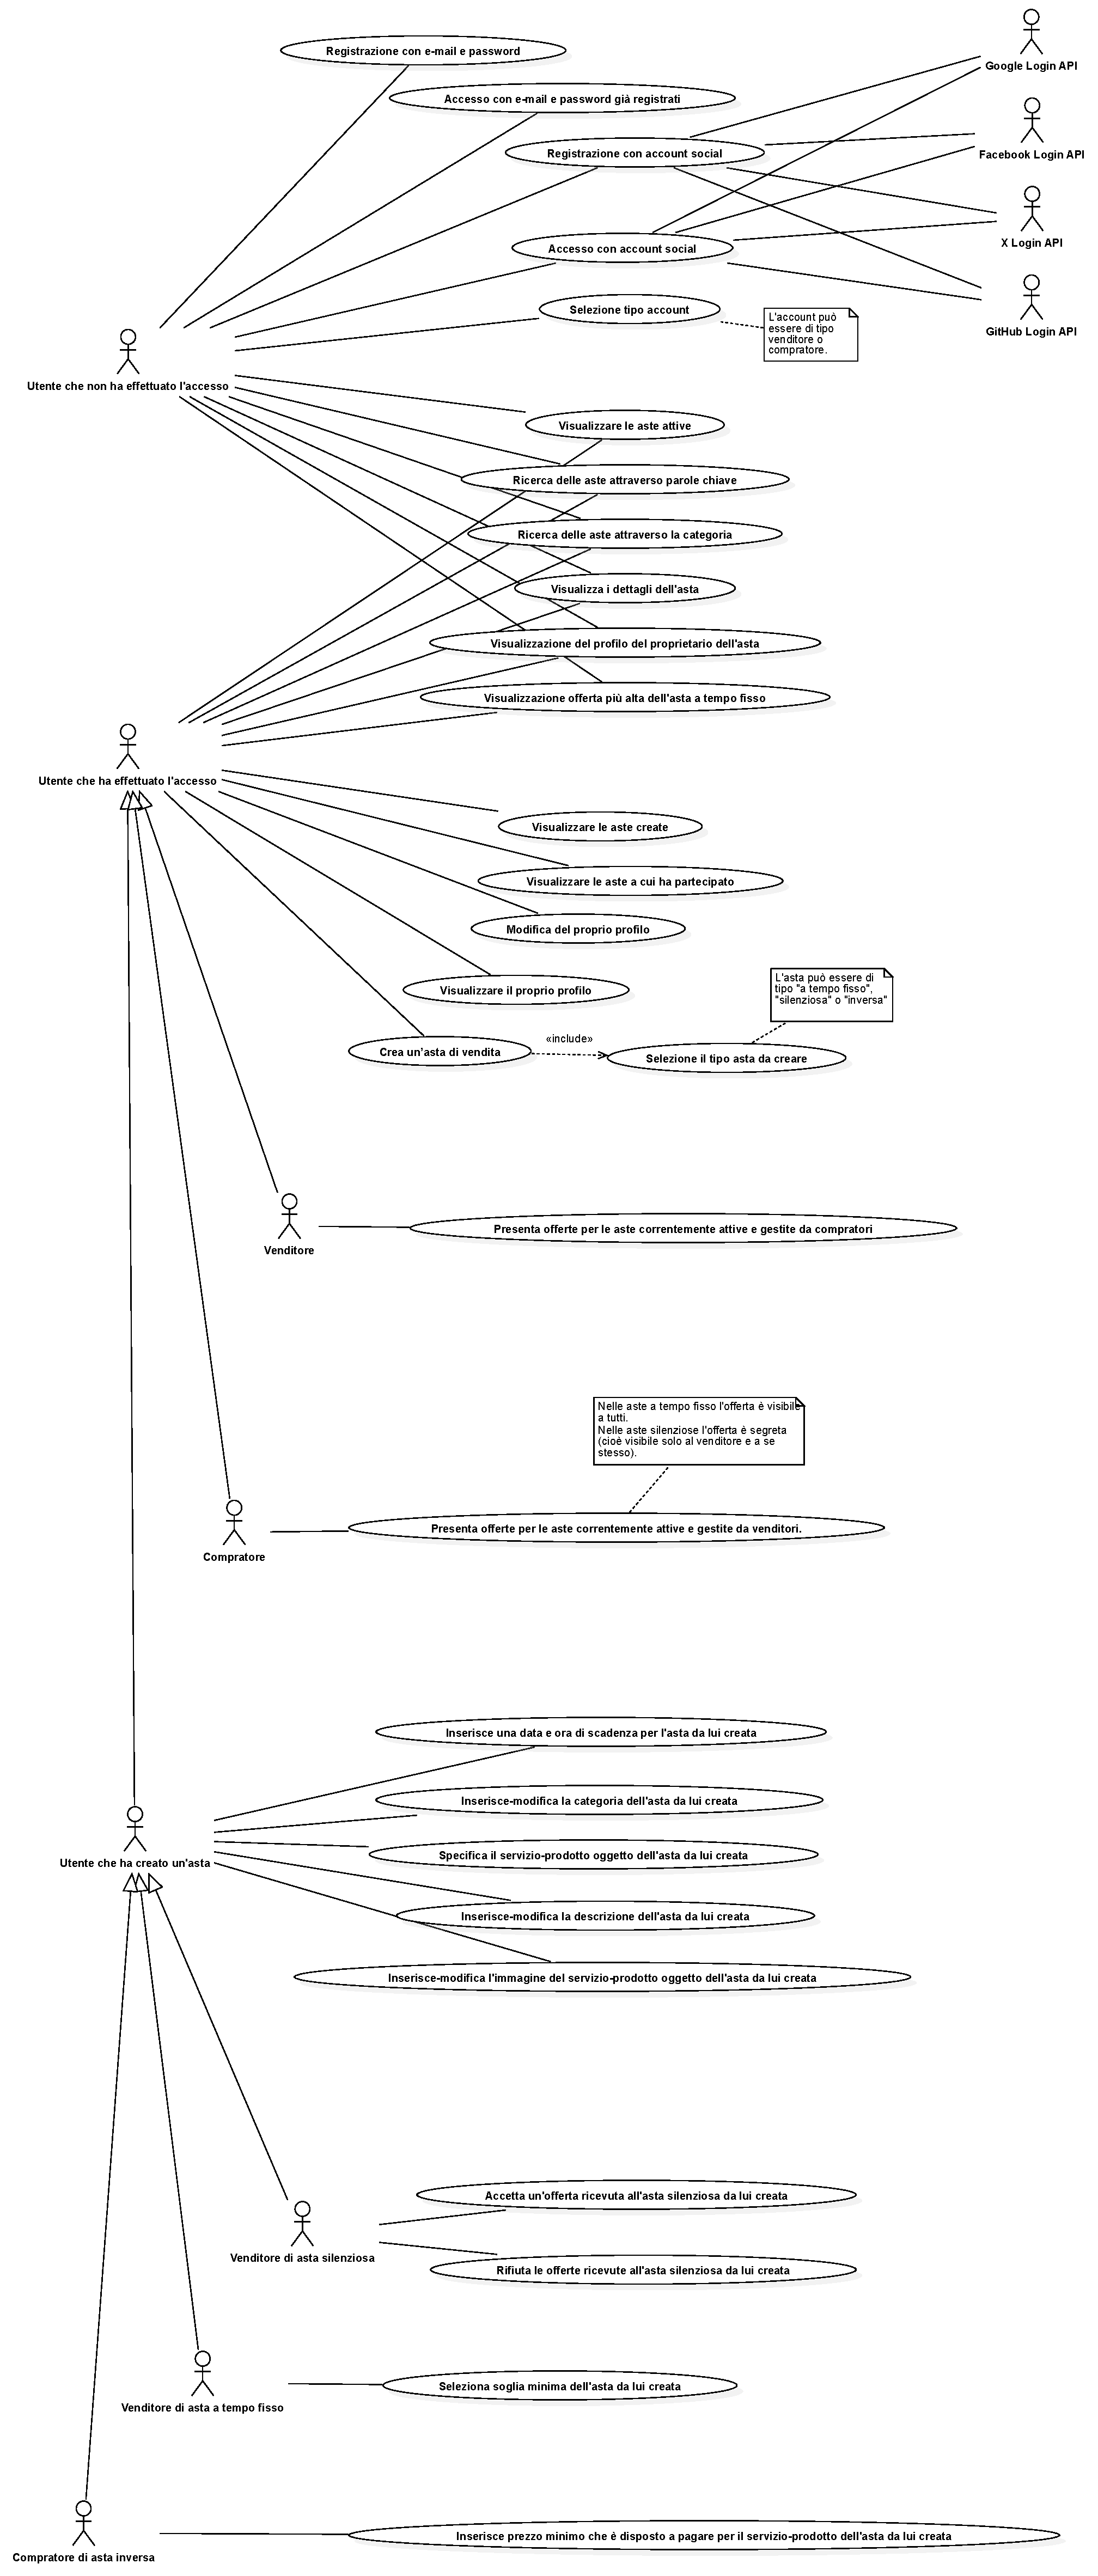
\includegraphics[width=0.42\linewidth]{Immagini/Diagrammi/UseCaseDiagram.pdf}
            \caption{Use Case Diagram}
            \label{fig:Use Case Diagram}
        \end{figure}

    \newpage
    
    \section{Target utenti}
        La personas principale scelta è Maria Lombardo. La personas secondaria è Luca Serra
        
        \begin{figure}[!htb]
           \begin{minipage}{0.48\textwidth}
                \centering
             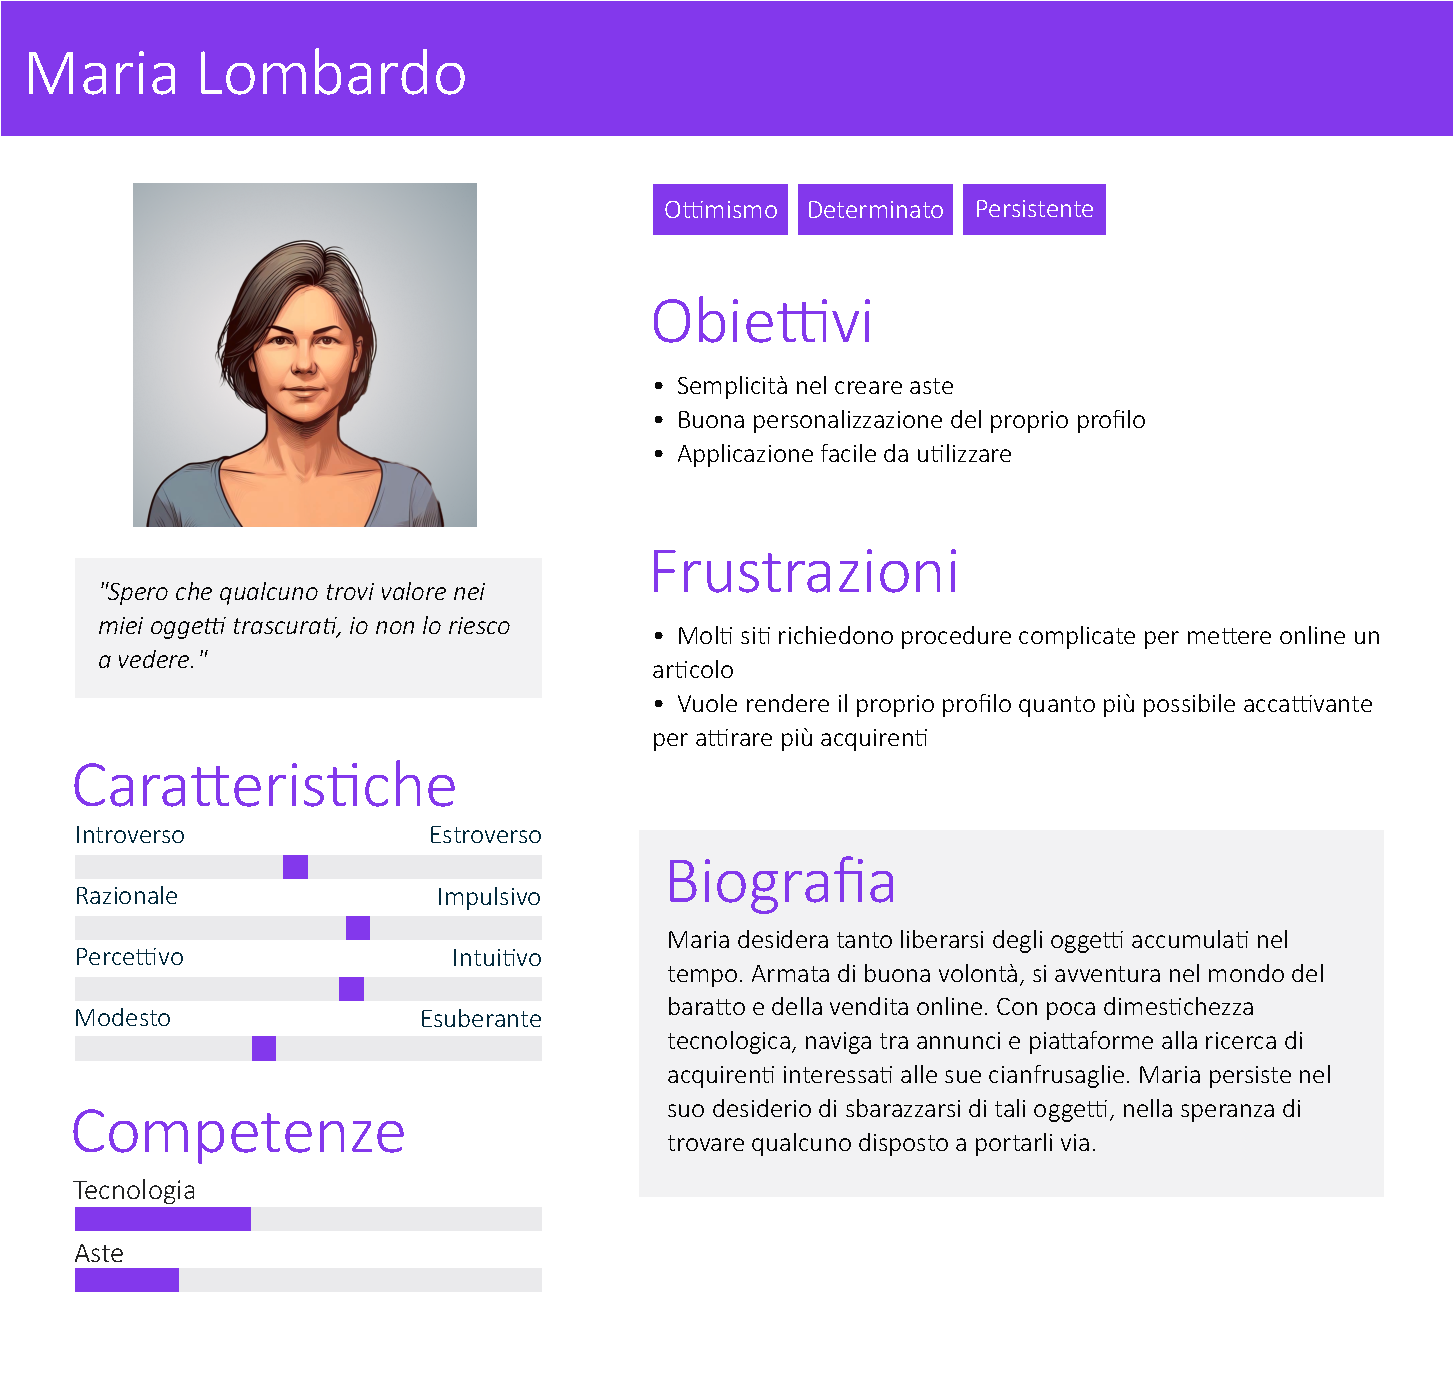
\includegraphics[width=.7\linewidth]{Immagini/Personas/Maria Lombardo.pdf}
             \caption{Maria Lombardo}\label{Fig:Maria Lombardo}
           \end{minipage}\hfill
           \begin{minipage}{0.48\textwidth}
                \centering
             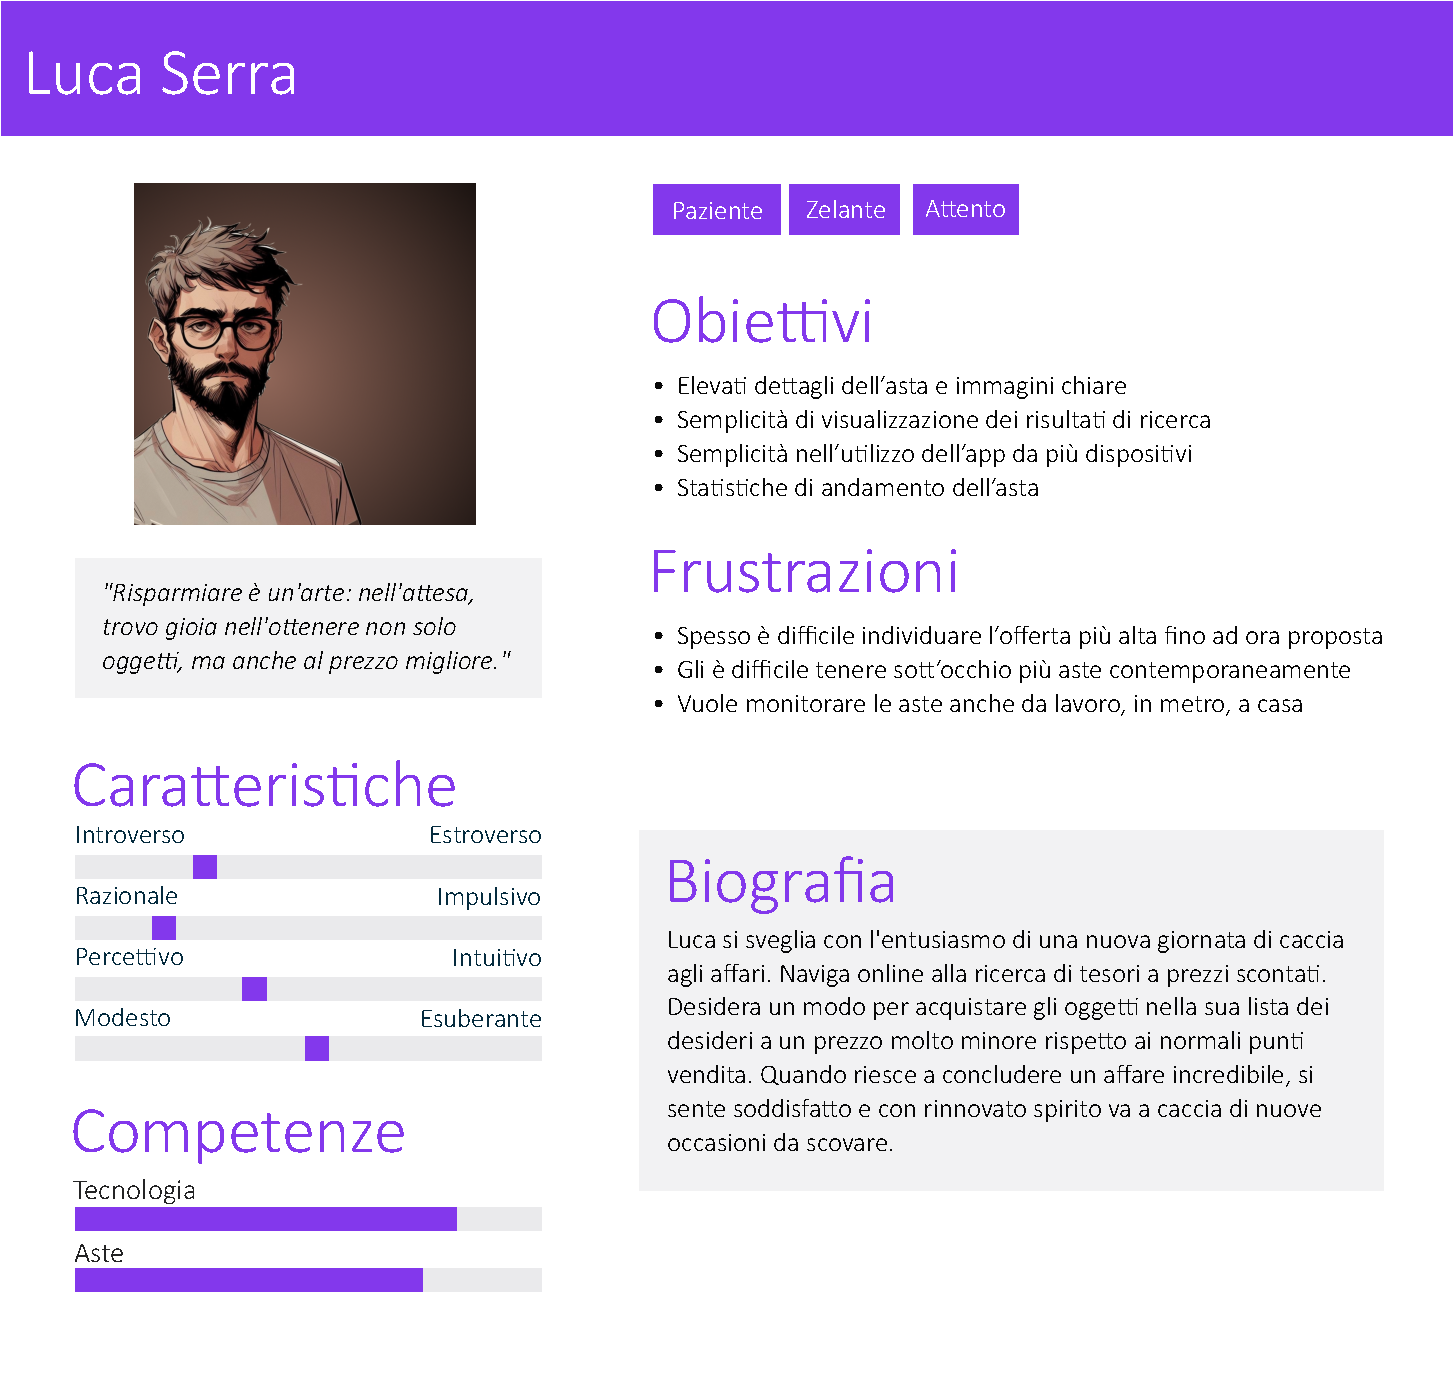
\includegraphics[width=.7\linewidth]{Immagini/Personas/Luca Serra.pdf}
             \caption{Luca Serra}\label{Fig:Luca Serra}
           \end{minipage}
        \end{figure}

        \begin{figure}[!htb]
           \begin{minipage}{0.48\textwidth}
                \centering
             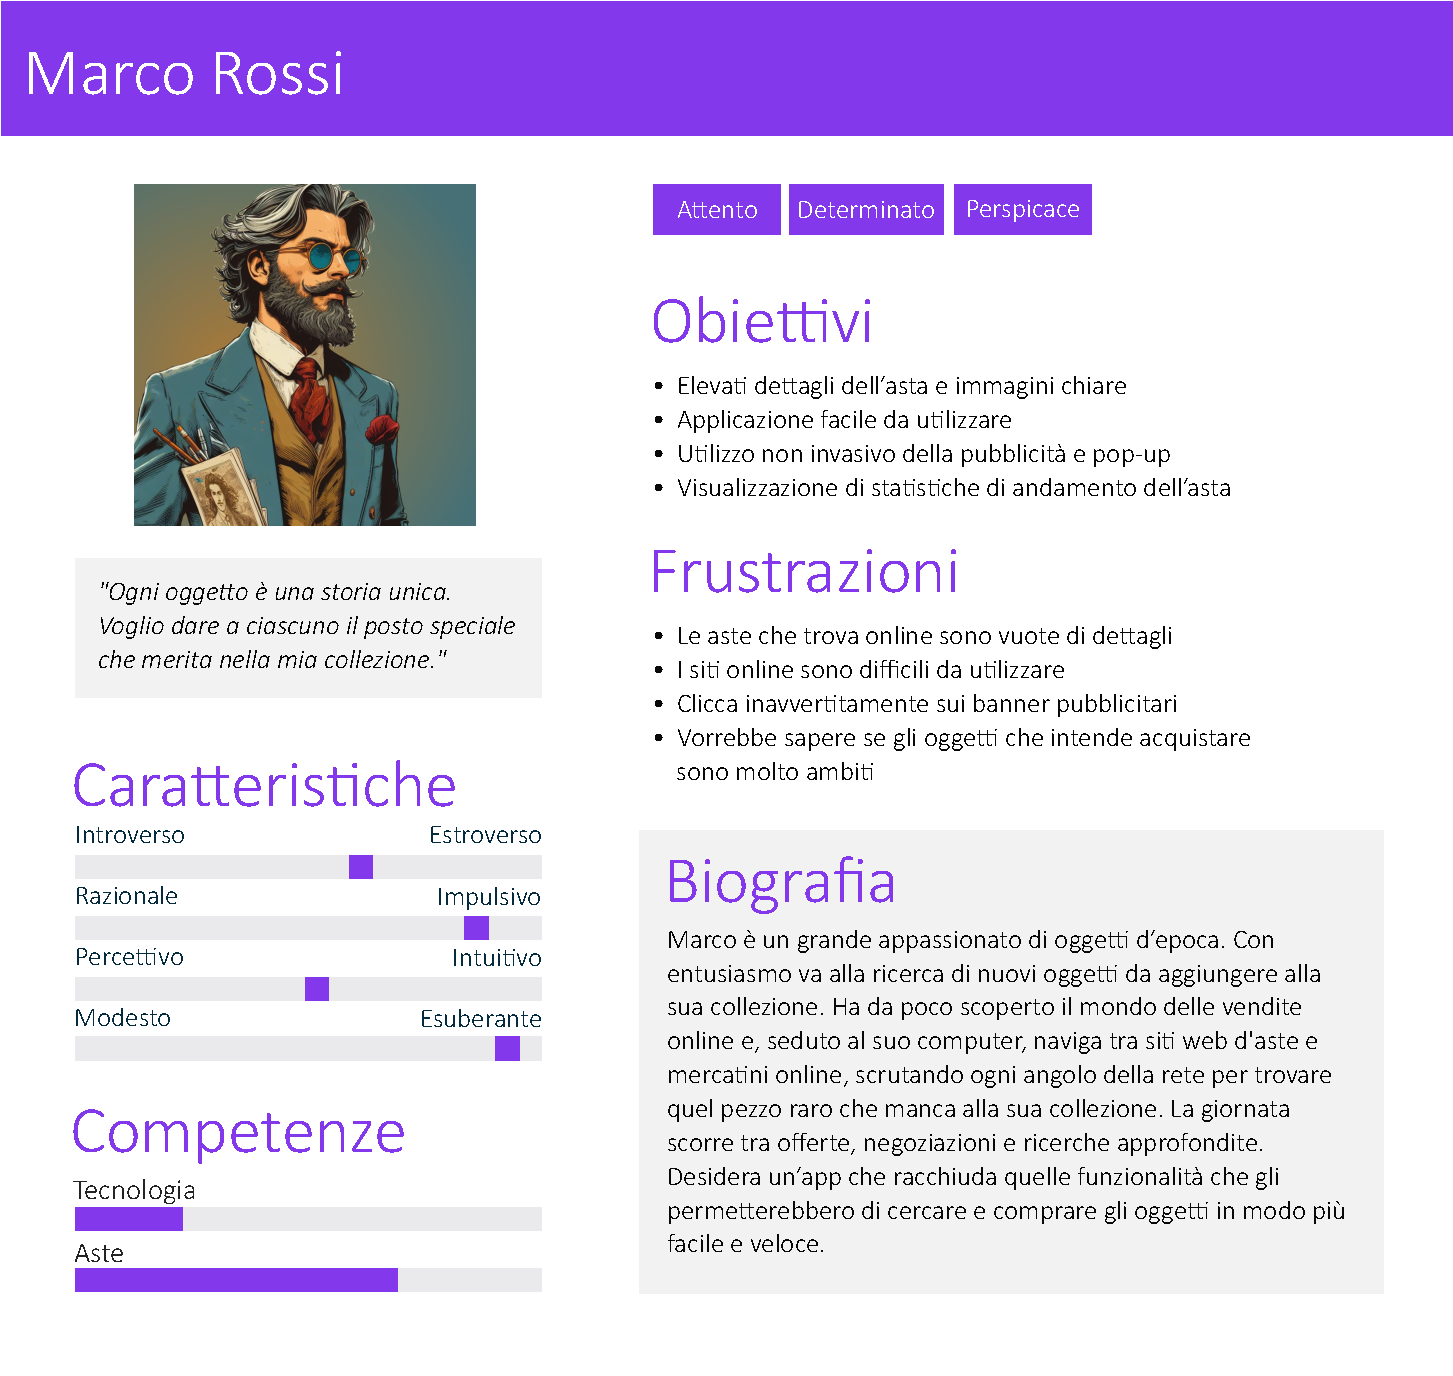
\includegraphics[width=.7\linewidth]{Immagini/Personas/Marco Rossi.pdf}
             \caption{Marco Rossi}\label{Fig:Marco Rossi}
           \end{minipage}\hfill
           \begin{minipage}{0.48\textwidth}
                \centering
             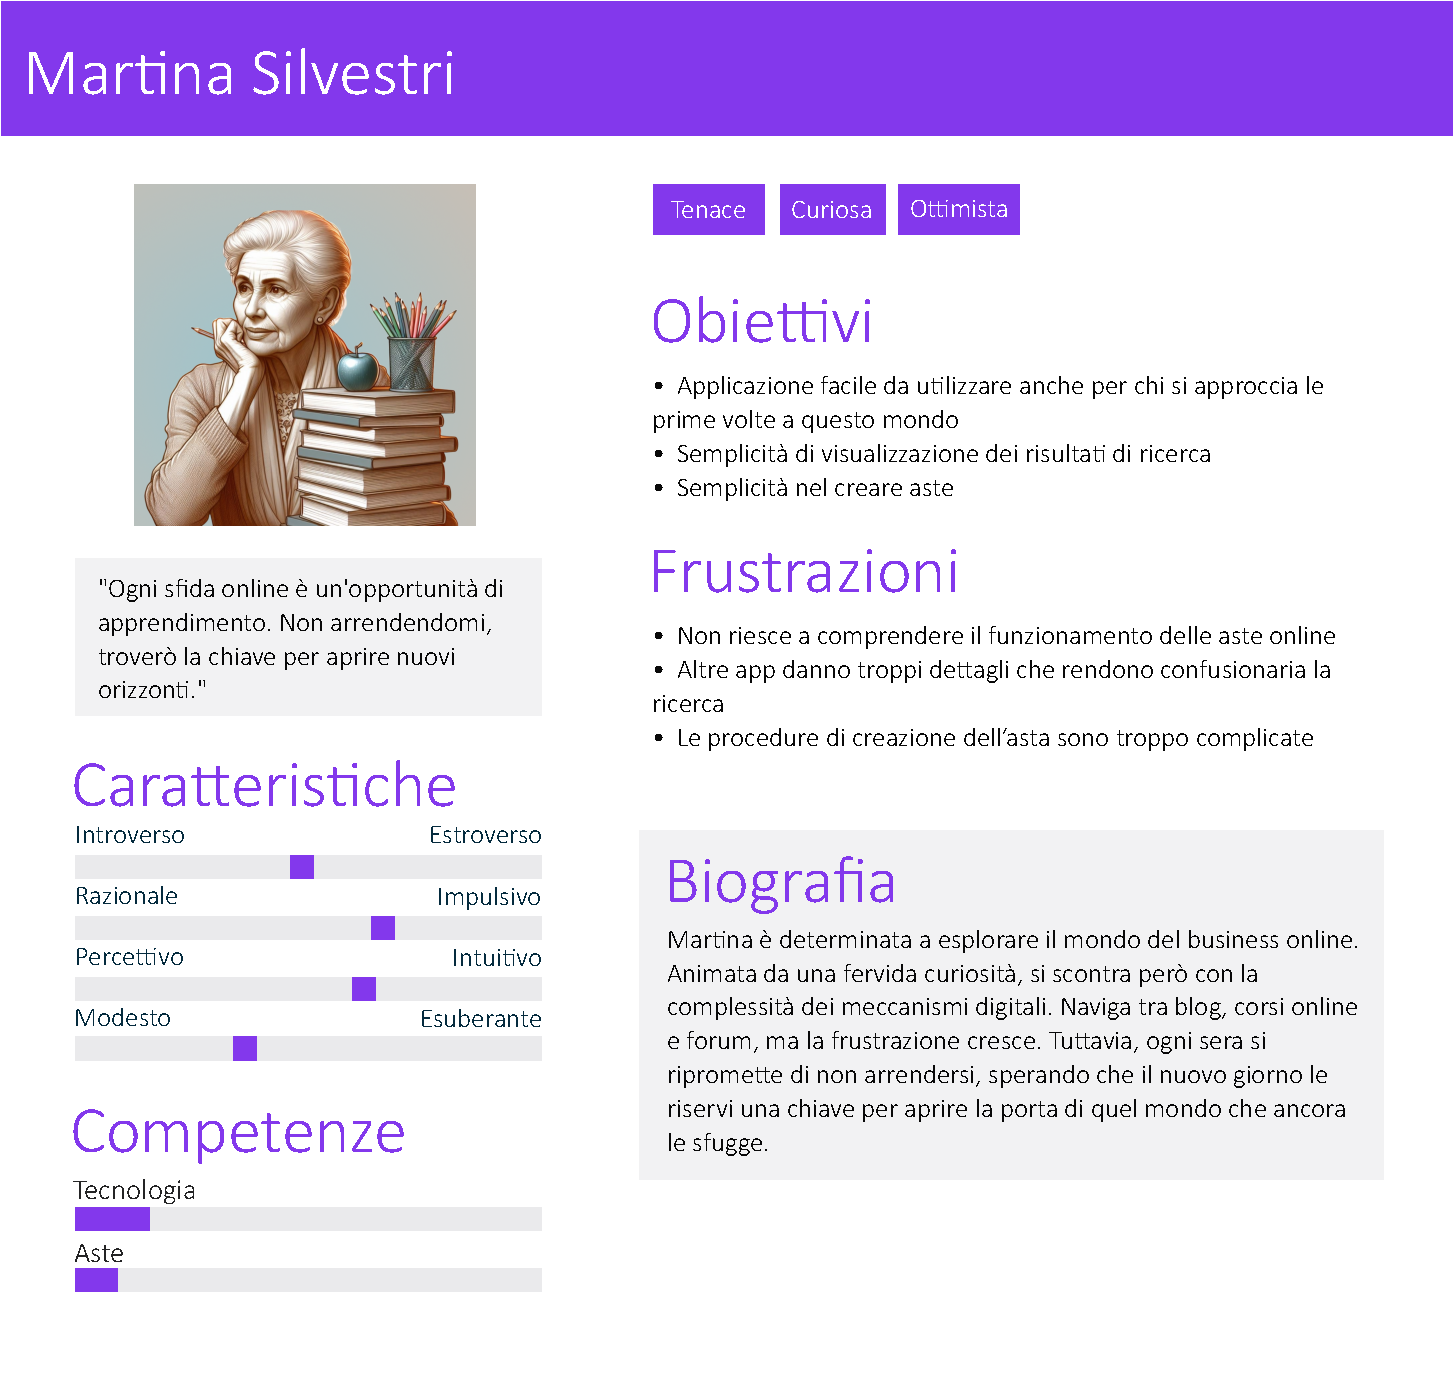
\includegraphics[width=.7\linewidth]{Immagini/Personas/Martina Silvestri.pdf}
             \caption{Martina Silvestri}\label{Fig:Martina Silvestri}
           \end{minipage}
        \end{figure}

        \begin{figure}[!htb]
           \begin{minipage}{0.48\textwidth}
                \centering
             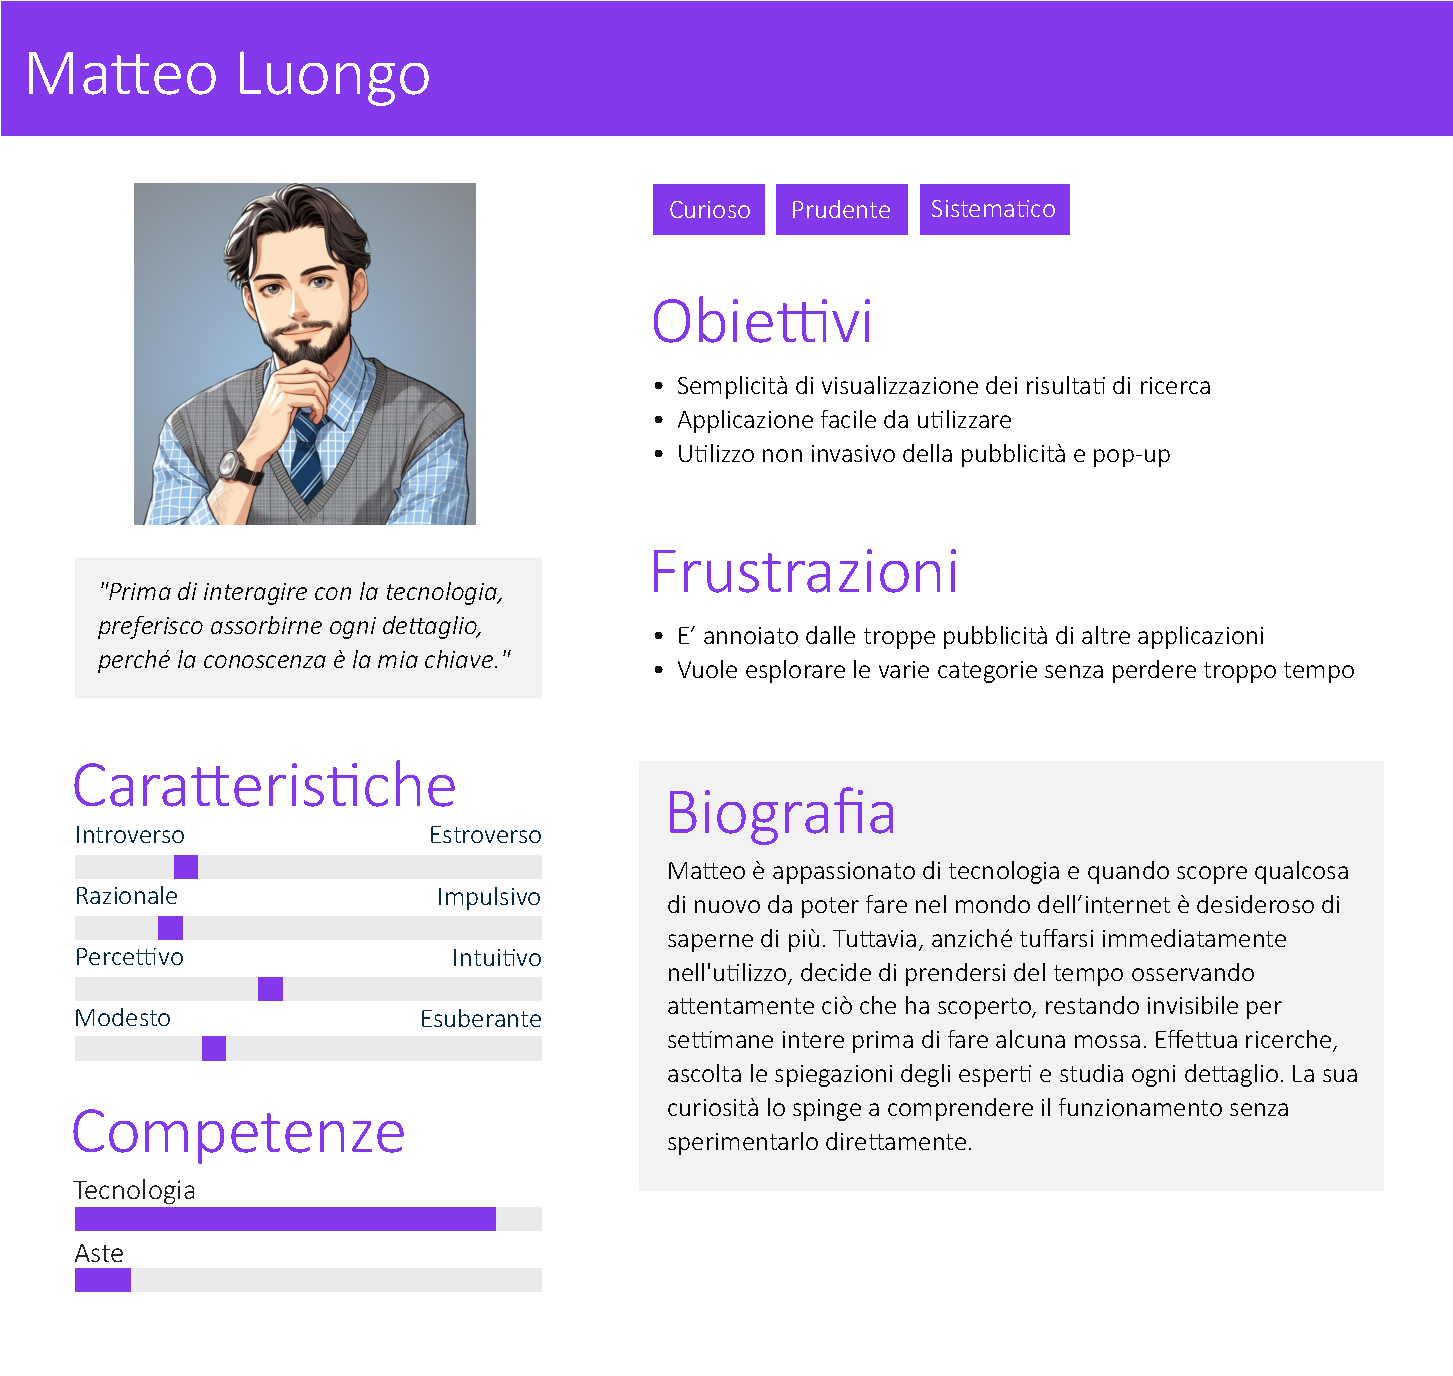
\includegraphics[width=.7\linewidth]{Immagini/Personas/Matteo Luongo.pdf}
             \caption{Matteo Luongo}\label{Fig:Matteo Luongo}
           \end{minipage}\hfill
           \begin{minipage}{0.48\textwidth}
                \centering
             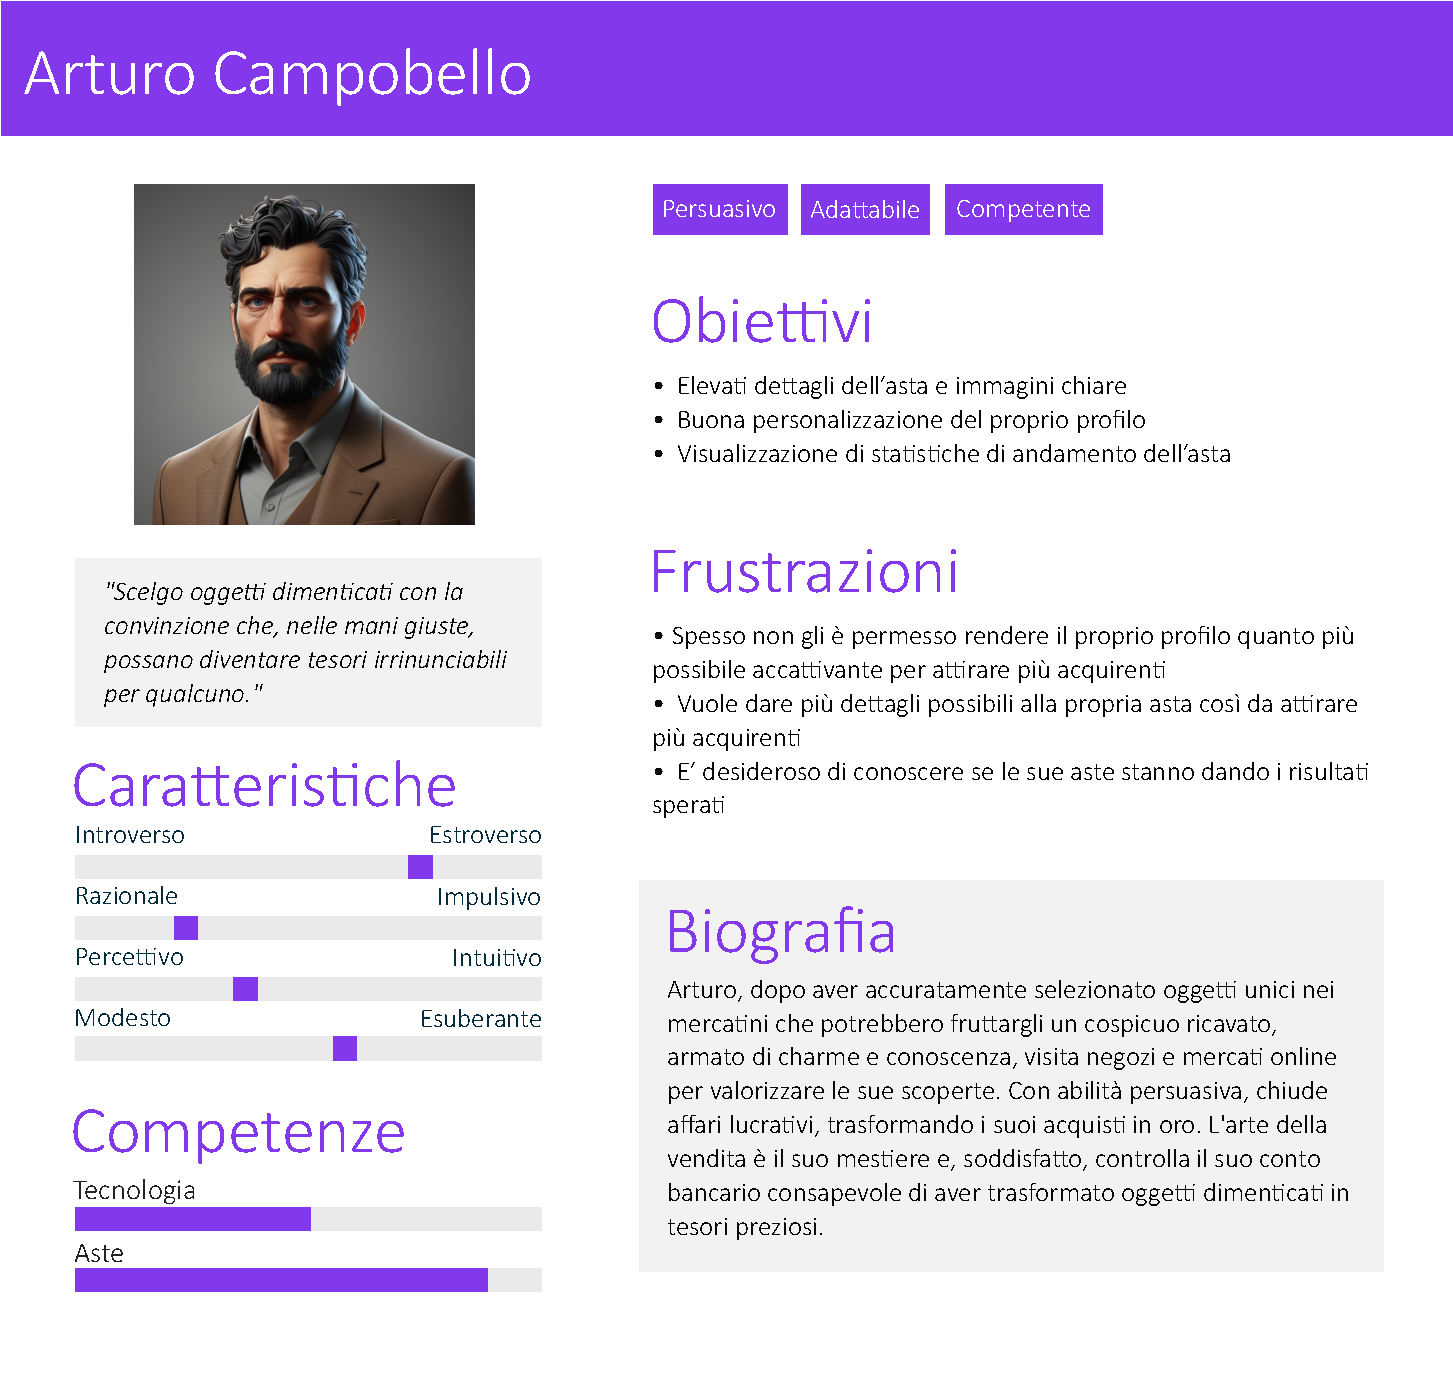
\includegraphics[width=.7\linewidth]{Immagini/Personas/Arturo Campobello.pdf}
             \caption{Arturo Campobello}\label{Fig:Arturo Campobello}
           \end{minipage}
        \end{figure}
        
    \section{Mockup}

    \newpage

    \section{Tabelle di Cockburn}
        \subsection{Crea un’asta inversa}
            \begin{longtable}{|C{3.0cm}|C{1.3cm}|L{5.2cm}|L{5.2cm}|}
                \hline
                    \textbf{USE CASE \#1} &
                    \multicolumn{3}{|l|}{\textbf{Crea un’asta inversa}}\\
                \hline
                    Goal in Context &
                    \multicolumn{3}{|l|}{L'utente di tipo "compratore" vuole creare un'asta inversa.}\\
                \hline
                    Preconditions &
                    \multicolumn{3}{|l|}{L'utente ha effettuato l'accesso con un account di tipo "compratore".}\\
                \hline
                    Success End Condition &
                    \multicolumn{3}{|l|}{L'utente di tipo "compratore" ha correttamente creato un'asta "inversa"}\\
                \hline
                    \multirow[|c|]{30}{*}{DESCRIPTION} 
                    & \textbf{Step n°}
                    & \textbf{Compratore}
                    & \textbf{Sistema}\\
                \cline{2-4}
                        & 1
                        & Preme bottone "Crea asta" su Mockup 6
                        & \\
                \cline{2-4}
                        & 2
                        & 
                        & Mostra Mockup 12 con tutte le informazioni dell'asta da poter inserire.\\
                \cline{2-4}
                        & 3
                        & Preme sul campo di input "Data di scadenza"
                        & \\
                \cline{2-4}
                        & 4
                        & 
                        & Mostra il pannello di selezione della data da calendario\\
                \cline{2-4}
                        & 5
                        & Seleziona la data
                        & \\
                \cline{2-4}
                        & 6
                        & Clicca su OK
                        & \\
                \cline{2-4}
                        & 7
                        & 
                        & Scrive la data selezionata nel campo di input "Data di scadenza"\\
                \cline{2-4}
                        & 8
                        & Preme sul campo di input "Ora di scadenza"
                        & \\
                \cline{2-4}
                        & 9
                        & 
                        & Mostra il pannello di selezione dell'ora\\
                \cline{2-4}
                        & 10
                        & Seleziona l'ora
                        & \\
                \cline{2-4}
                        & 11
                        & Clicca su OK
                        & \\
                \cline{2-4}
                        & 12
                        & 
                        & Scrive l'ora selezionata nel campo di input "Ora di scadenza"\\
                \cline{2-4}
                        & 13
                        & Preme sul campo di input "Prezzo di partenza"
                        & \\
                \cline{2-4}
                        & 14
                        &
                        & Mostra il tastierino numerico \\
                \cline{2-4}
                        & 15
                        & Inserisce il prezzo di partenza
                        & \\
                \cline{2-4}
                        & 16
                        & Preme sul campo di input "Nome prodotto"
                        & \\
                \cline{2-4}
                        & 17
                        &
                        & Mostra la tastiera \\
                \cline{2-4}
                        & 18
                        & Inserisce il nome del prodotto oggetto dell'asta
                        & \\
                \cline{2-4}
                        & 19
                        & Preme sul campo di input "Categoria"
                        & \\
                \cline{2-4}
                        & 20
                        &
                        & Mostra il menù a tendina con le diverse categorie tra cui scegliere \\
                \cline{2-4}
                        & 21
                        & Seleziona la categoria
                        & \\
                \cline{2-4}
                        & 22
                        & 
                        & Scrive la categoria scelta nel campo di input "Categoria"\\
                \cline{2-4}
                        & 23
                        & Preme sul campo di input "Descrizione"
                        & \\
                \cline{2-4}
                        & 24
                        &
                        & Mostra la tastiera \\
                \cline{2-4}
                        & 25
                        & Inserisce la descrizione del prodotto oggetto dell'asta
                        & \\
                \cline{2-4}
                        & 26
                        & Preme sul pulsante "Crea"
                        & \\
                \cline{2-4}
                        & 27
                        & 
                        & Mostra Mockup P29 (Pop-up di successo)\\
                \cline{2-4}
                        & 28
                        & Preme il pulsante X sul Mockup P29
                        & \\
                \cline{2-4}
                        & 29
                        & 
                        & Torna al Mockup 6 (Home)\\
                \hline
                    EXTENSIONS
                    & \textbf{Step n°} 
                    & \textbf{Compratore} 
                    & \textbf{Sistema}\\
                \hline
                    \multirow[|c|]{3}{*}{\shortstack[c]{Seleziona data \\  antecedente a \\quella odierna}}
                        & 7.a
                        & 
                        & Mostra Mockup P37 con testo "Non puoi inserire una data antecedente a quella odierna!"\\
                \cline{2-4}
                        & 8.a
                        & Clicca su X
                        & \\
                \cline{2-4}
                        & 9.a
                        & 
                        & Continua da step 3 di main scenario\\
                \hline
                    \multirow[|c|]{3}{*}{\shortstack[c]{Seleziona data \\ odierna e ora \\ antecedente a \\quella attuale}}
                        & 12.a
                        & 
                        & Mostra Mockup P28 con testo "Non puoi selezionare un’ora antecedente a quella attuale in data odierna!"\\
                \cline{2-4}
                        & 13.a
                        & Clicca su X
                        & \\
                \cline{2-4}
                        & 14.a
                        & 
                        & Continua da step 8 di main scenario\\
                \hline
                    \multirow[|c|]{3}{*}{\shortstack[c]{Seleziona prezzo di \\ partenza negativo}}
                        & 16.b
                        & 
                        & Mostra Mockup P24 con testo "Non puoi inserire una somma di partenza minore di 0 €."\\
                \cline{2-4}
                        & 17.b
                        & Clicca su X
                        & \\
                \cline{2-4}
                        & 16.b
                        & 
                        & Continua da step 13 di main scenario\\
                \hline
                    \multirow[|c|]{2}{*}{\shortstack[c]{Alcuni campi \\ obbligatori non \\ compilati}}
                        & 27.c
                        & 
                        & Mostra Mockup E11 dove vengono segnalati in rosso i campi obbligatori non compilati\\
                \cline{2-4}
                        & 28.c
                        & Riparte da step 3 di main scenario, saltando i campi di input già compilati
                        & \\
                \hline
                    \multirow[|c|]{4}{*}{\shortstack[c]{Esce dalla pagina \\ di creazione asta}}
                        & \textit{In qualunque passo del main scenario}
                        & Preme qualsiasi tasto di navigazione (della navbar in basso o tasto "indietro" del dispositivo)
                        & \\
                \cline{2-4}
                        & 
                        & 
                        & Mostra Mockup P33 con testo "Se uscirai da questa schermata, i dati inseriti nei campi saranno cancellati. Vuoi proseguire?" \\
                \cline{2-4}
                        & 
                        & Clicca su Esci
                        & \\
                \cline{2-4}
                        & 
                        & 
                        & Mostra Mockup corrispondente al tasto cliccato\\
                \hline
                    SUBVARIATIONS
                    & \textbf{Step n°} 
                    & \textbf{Compratore} 
                    & \textbf{Sistema}\\
                \hline
                    \multirow[|c|]{1}{*}{\shortstack[c]{Inserisce immagine}}
                        & 16.s1
                        & Preme sul campo di input "Aggiungi immagine prodotto"
                        & \\
                \cline{2-4}
                        & 17.s1
                        & 
                        & Mostra il sistema per selezionare le immagini\\
                \cline{2-4}
                        & 18.s1
                        & Seleziona una o più immagini
                        & \\
                \cline{2-4}
                        & 19.s1
                        & Clicca su OK
                        & \\
                \cline{2-4}
                        & 20.s1
                        & 
                        & Continua da step 16 di main scenario\\
                \hline
            \end{longtable}

        \newpage

        \subsection{Accetta un'offerta ricevuta all'asta silenziosa}
            \begin{longtable}{|C{3.0cm}|C{1.3cm}|L{5.2cm}|L{5.2cm}|}
                \hline
                    \textbf{USE CASE \#2} &
                    \multicolumn{3}{|l|}{\textbf{Accetta un'offerta ricevuta all'asta silenziosa}}\\
                \hline
                    Goal in Context &
                    \multicolumn{3}{|l|}{\shortstack[l]{L'utente di tipo "venditore" vuole accettare un'offerta ricevuta in un'asta \\ "silenziosa" da lui creata}}\\
                \hline
                    Preconditions &
                    \multicolumn{3}{|l|}{\shortstack[l]{L'utente ha effettuato l'accesso con un account di tipo "venditore" e ha creato \\ un'asta "silenziosa"}}\\
                \hline
                    Success End Condition &
                    \multicolumn{3}{|l|}{\shortstack[l]{L'utente di tipo "venditore" ha correttamente accettato un'offerta di un'asta \\ "silenziosa" da lui creata}}\\
                \hline
                    \multirow[|c|]{11}{*}{DESCRIPTION} 
                    & \textbf{Step n°}
                    & \textbf{Venditore di asta silenziosa}
                    & \textbf{Sistema}\\
                \cline{2-4}
                        & 1
                        & Preme bottone "Profilo" su Mockup 10
                        & \\
                \cline{2-4}
                        & 2
                        & 
                        & Mostra Mockup 18 con tutte le opzioni per utenti loggati.\\
                \cline{2-4}
                        & 3
                        & Preme sul bottone "Le mie aste create".
                        & \\
                \cline{2-4}
                        & 4
                        & 
                        & Mostra il Mockup 27 con tutte le aste create dal venditore.\\
                \cline{2-4}
                        & 5
                        & Clicca sull'icona a forma di elenco dell'asta di cui si vogliono visualizzare le offerte ricevute.
                        & \\
                \cline{2-4}
                        & 6
                        & 
                        & Mostra Mockup 31 con l'elenco di tutte le offerte ricevute.\\
                \cline{2-4}
                        & 7
                        & Clicca sulla spunta verde dell'offerta che si vuole accettare.
                        & \\
                \cline{2-4}
                        & 8
                        & 
                        & Mostra il Mockup P9 con testo "Confermi di voler accettare questa offerta? Tutte le altre saranno automaticamente rifiutate."\\
                \cline{2-4}
                        & 9
                        & Clicca sul pulsante "Accetta"
                        & \\
                \cline{2-4}
                        & 10
                        & 
                        & Mostra Mockup 32 dove vengono elencate tutte le offerte ricevute a questa asta "silenziosa". L'offerta accettata sarà l'unica in bianco, tutte le altre saranno in grigio.\\
                \hline
                    EXTENSIONS
                    & \textbf{Step n°} 
                    & \textbf{Venditore di asta silenziosa} 
                    & \textbf{Sistema}\\
                \hline
                    \multirow[|c|]{2}{*}{\shortstack[c]{Esce dalla pagina \\ di gestione delle \\ offerta ricevute}}
                        & 7.a
                        & Preme sul tasto "indietro" (del dispositivo o dell'interfaccia)
                        & \\
                \cline{2-4}
                        & 8.a
                        & 
                        & Mostra Mockup nel quale ci si trovava in precedenza\\
                \hline
                    SUBVARIATIONS
                    & \textbf{Step n°} 
                    & \textbf{Venditore di asta silenziosa}
                    & \textbf{Sistema}\\
                \hline
                    \multirow[|c|]{4}{*}{\shortstack[c]{Riceve notifica \\ di proposta offerta \\ per l'asta silenziosa}}
                        & 1.s1
                        & Preme sul bottone "Notifiche"
                        & \\
                \cline{2-4}
                        & 2.s1
                        & 
                        & Mostra il Mockup 34 con la notifica relativa all'offerta ricevuta\\
                \cline{2-4}
                        & 3.s1
                        & Clicca sul bottone relativo alla notifica
                        & \\
                \cline{2-4}
                        & 4.s1
                        &
                        & Continua con step 6 di main scenario\\
                \hline
            \end{longtable}
    %PDF DI RIFERIMENTO: 04_Modelli di Dominio.pdf, Statecharts.pdf

\chapter{Requirement Specification}
    \section{Obiettivo}
        I requisiti che sono stati riorganizzati nella fase di analisi sono formalizzati in diagrammi (diagramma di classe, diagramma di sequenza, diagramma degli stati) attraverso l'uso di linguaggi di modellazione come UML. \\
        Per individuare il modello ad oggetti per questo dominio, si è scelto di impiegare l'euristica "Three-Object-Type" perché permette di costruire un modello più flessibile e facile da modificare.

    \section{Class Diagram}
        Il Class Diagram individua quali sono le entità coinvolte all'interno del nostro dominio e le relazioni che tra esse sussistono.\\
        In particolare, il modello concettuale basato sull'analisi dei requisiti permetterà di creare un modello efficace per la gestione delle aste.\\
        \subsection{Class Diagram del dominio del problema}
            %Class Diagram costruito con StarUML
            \begin{figure}[htbp!]
                \centering
                    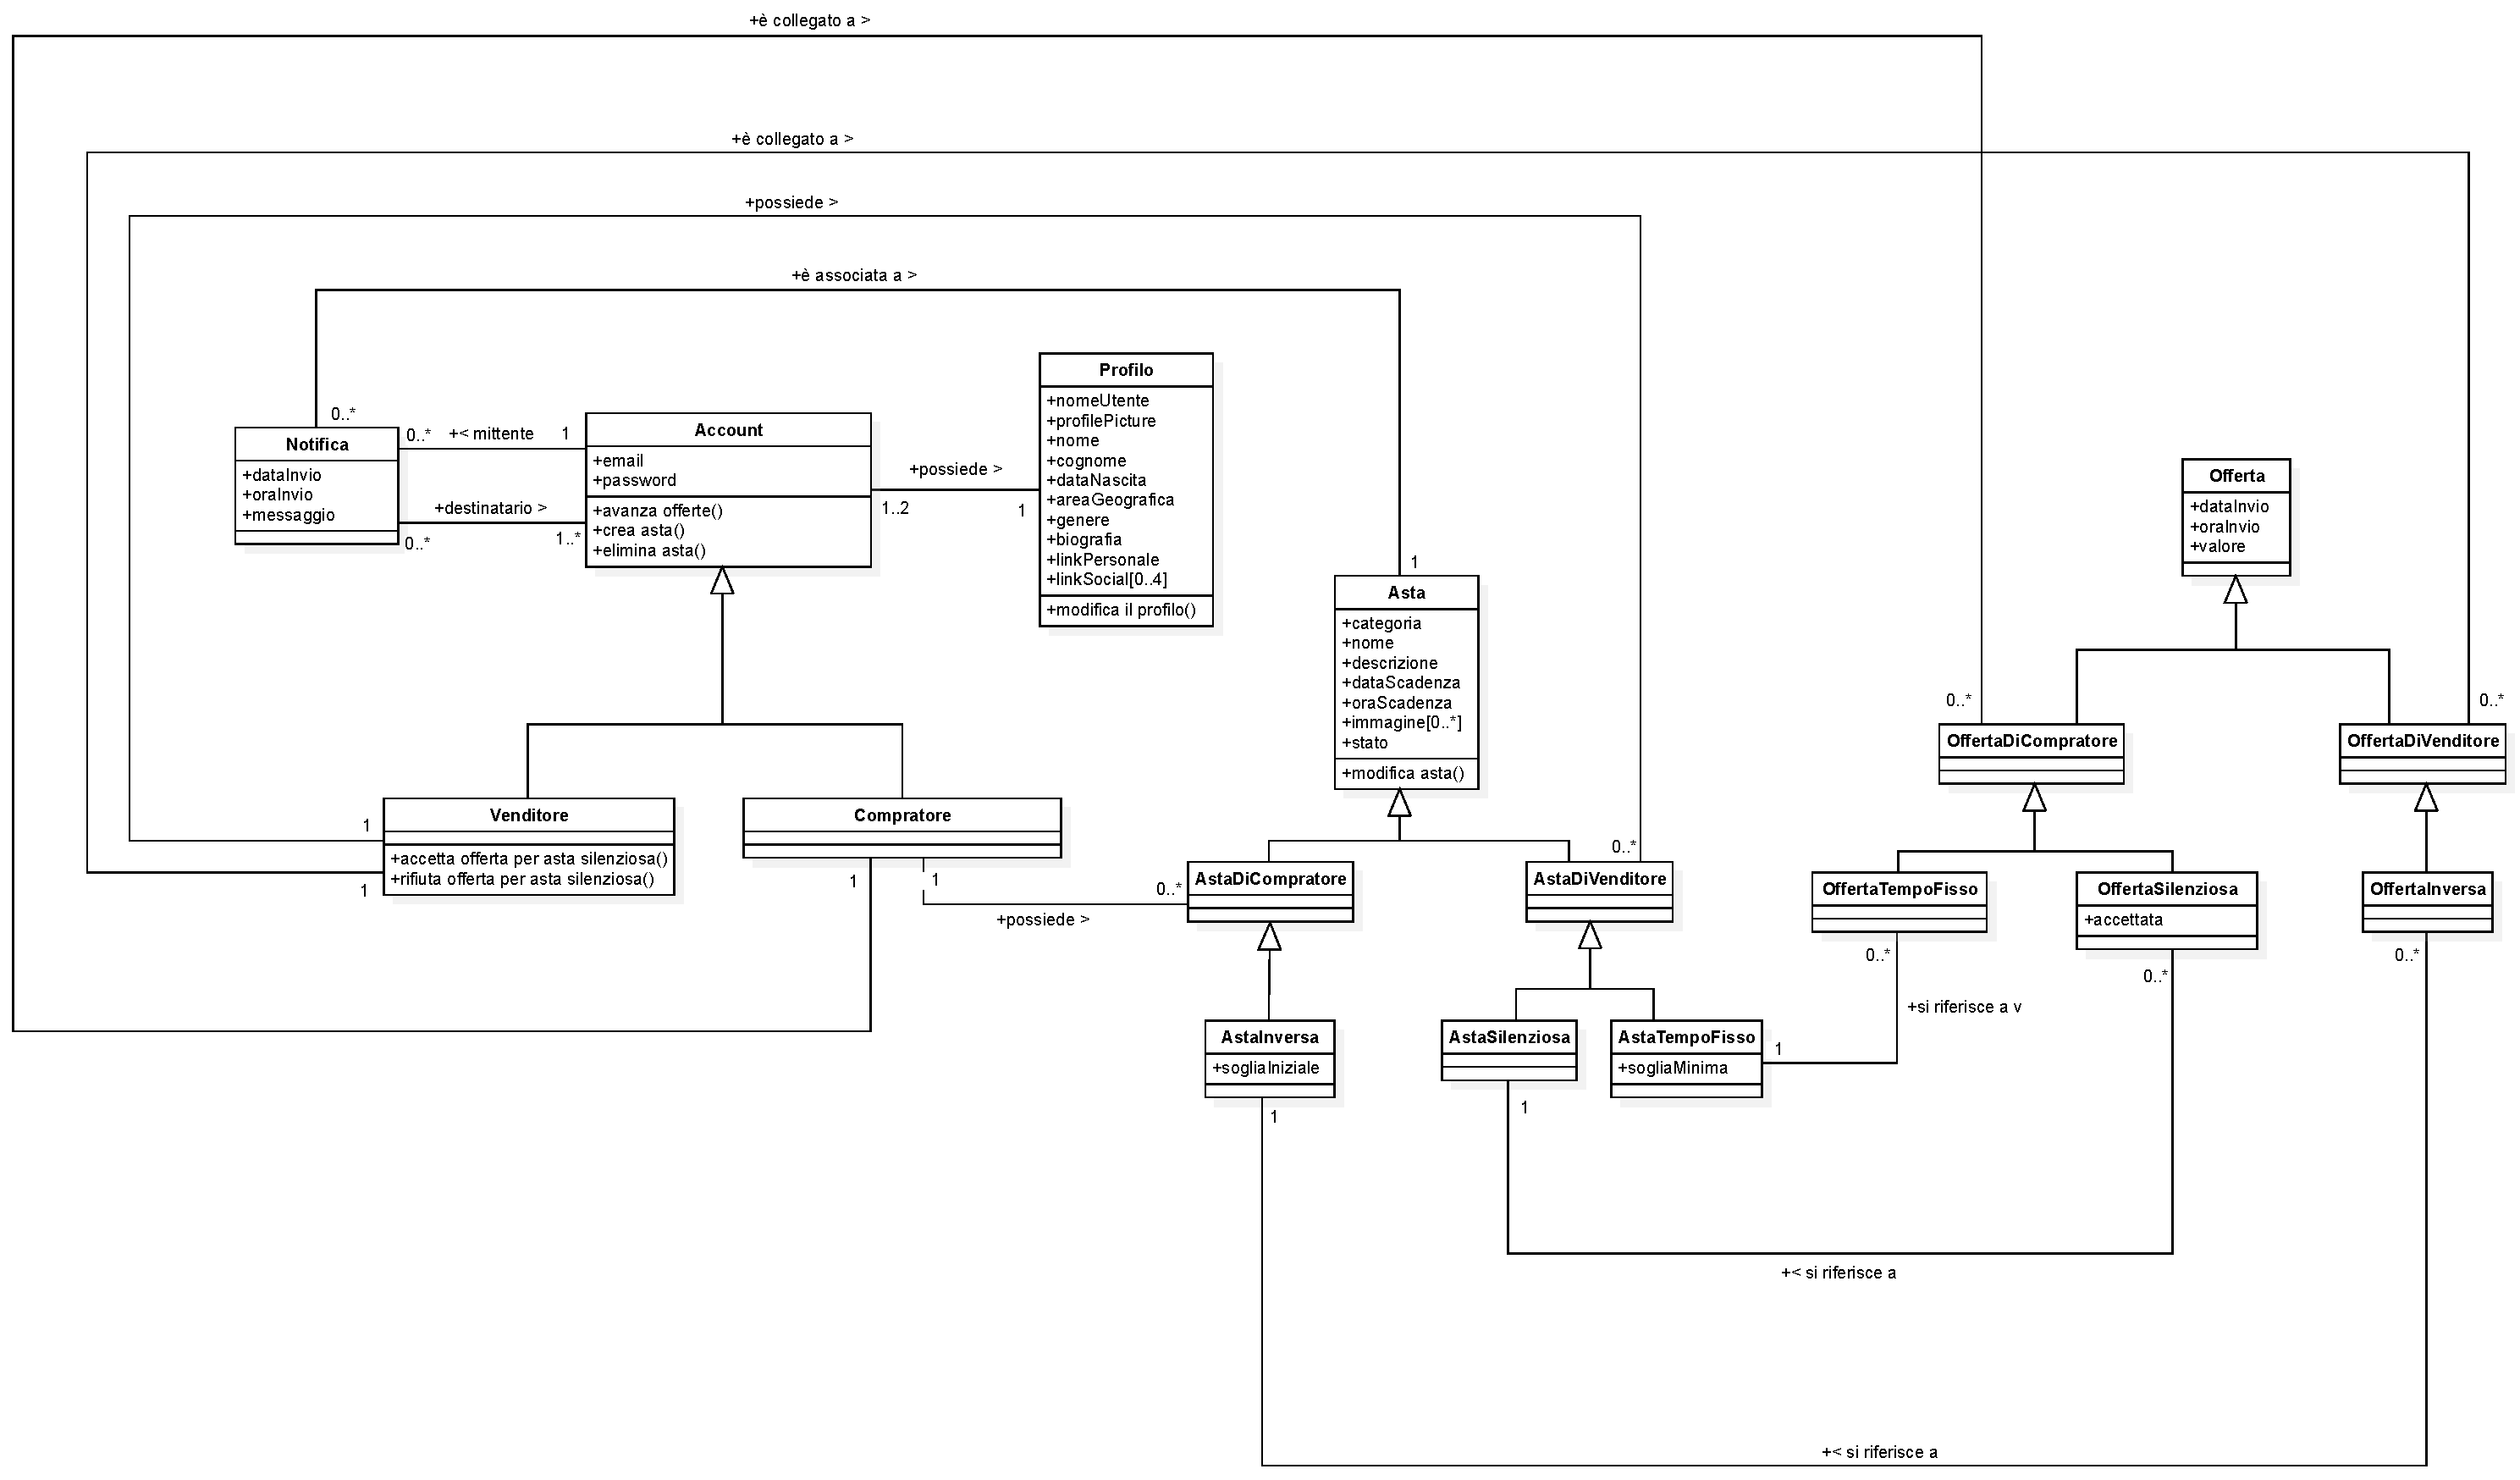
\includegraphics[width=1\linewidth]{Immagini/Diagrammi/Class Diagram/ClassDiagramDominio.pdf}
                \caption{Class Diagram del dominio del problema}
                \label{fig:Class Diagram del dominio del problema}
            \end{figure}
            
        \subsection{Class Diagram per casi d'uso}
            In questa sezione verranno mostrati i diagrammi secondo l'euristica "Three-Object-Type" per ogni caso d'uso. Le classi possono essere di tipo "boundary", "control" e "entity".
        
            \begin{figure}[htbp!]
                \centering
                    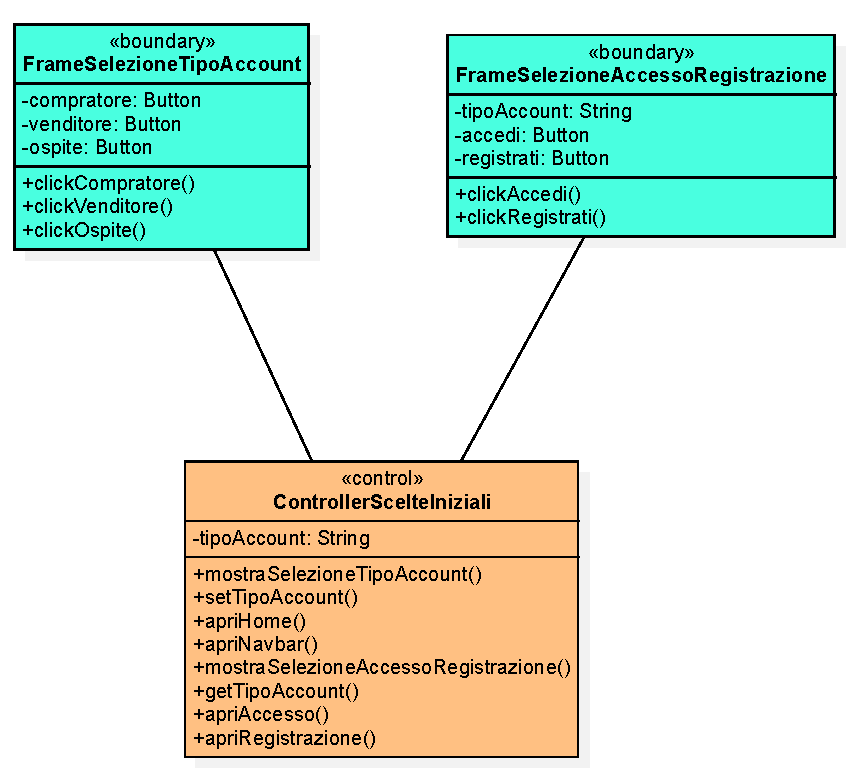
\includegraphics[width=1\linewidth]{Immagini/Diagrammi/Class Diagram/Utente che non ha effettuato l'accesso/ScelteIniziali.pdf}
                \caption{Scelta del tipo di account}
            \end{figure}
            
            \begin{figure}[htbp!]
                \centering
                    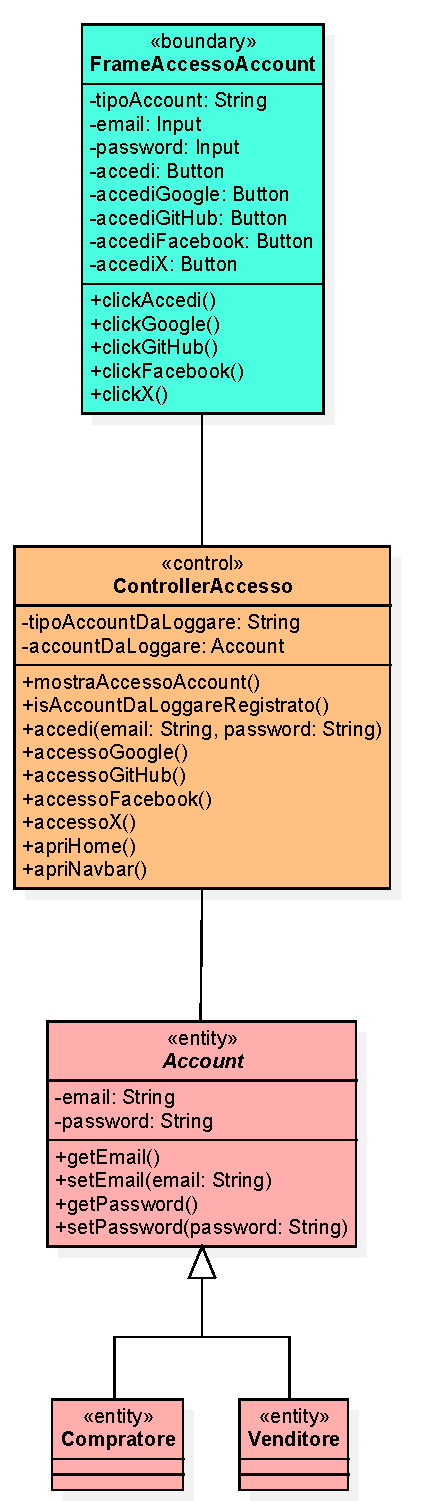
\includegraphics[width=0.35\linewidth]{Immagini/Diagrammi/Class Diagram/Utente che non ha effettuato l'accesso/Accesso.pdf}
                \caption{Accesso}
            \end{figure}
            
            \begin{figure}[htbp!]
                \centering
                    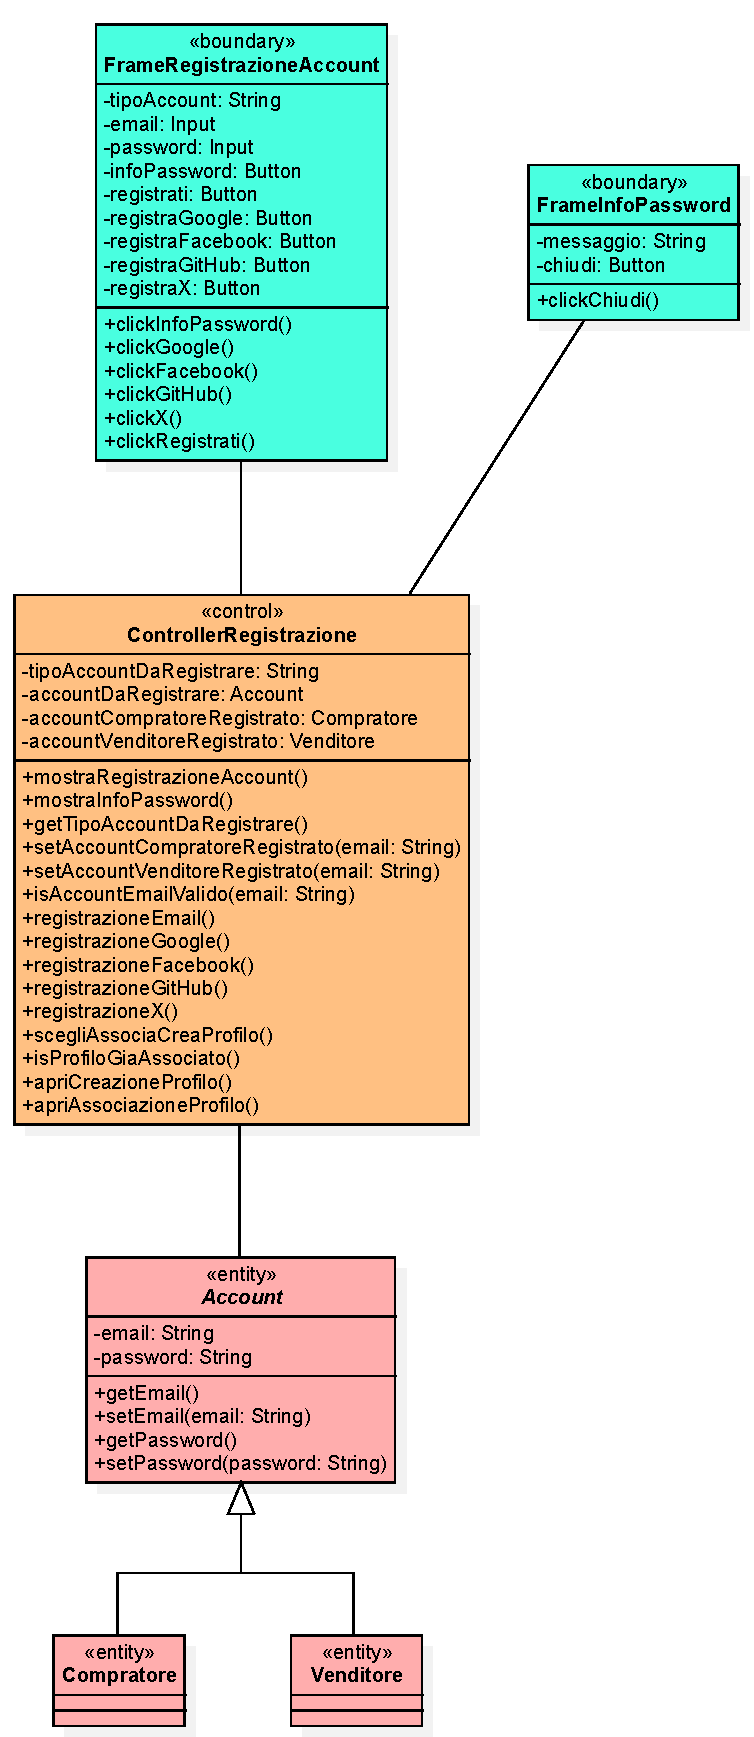
\includegraphics[width=0.55\linewidth]{Immagini/Diagrammi/Class Diagram/Utente che non ha effettuato l'accesso/Registrazione.pdf}
                \caption{Registrazione}
            \end{figure}
            
            \begin{figure}[htbp!]
                \centering
                    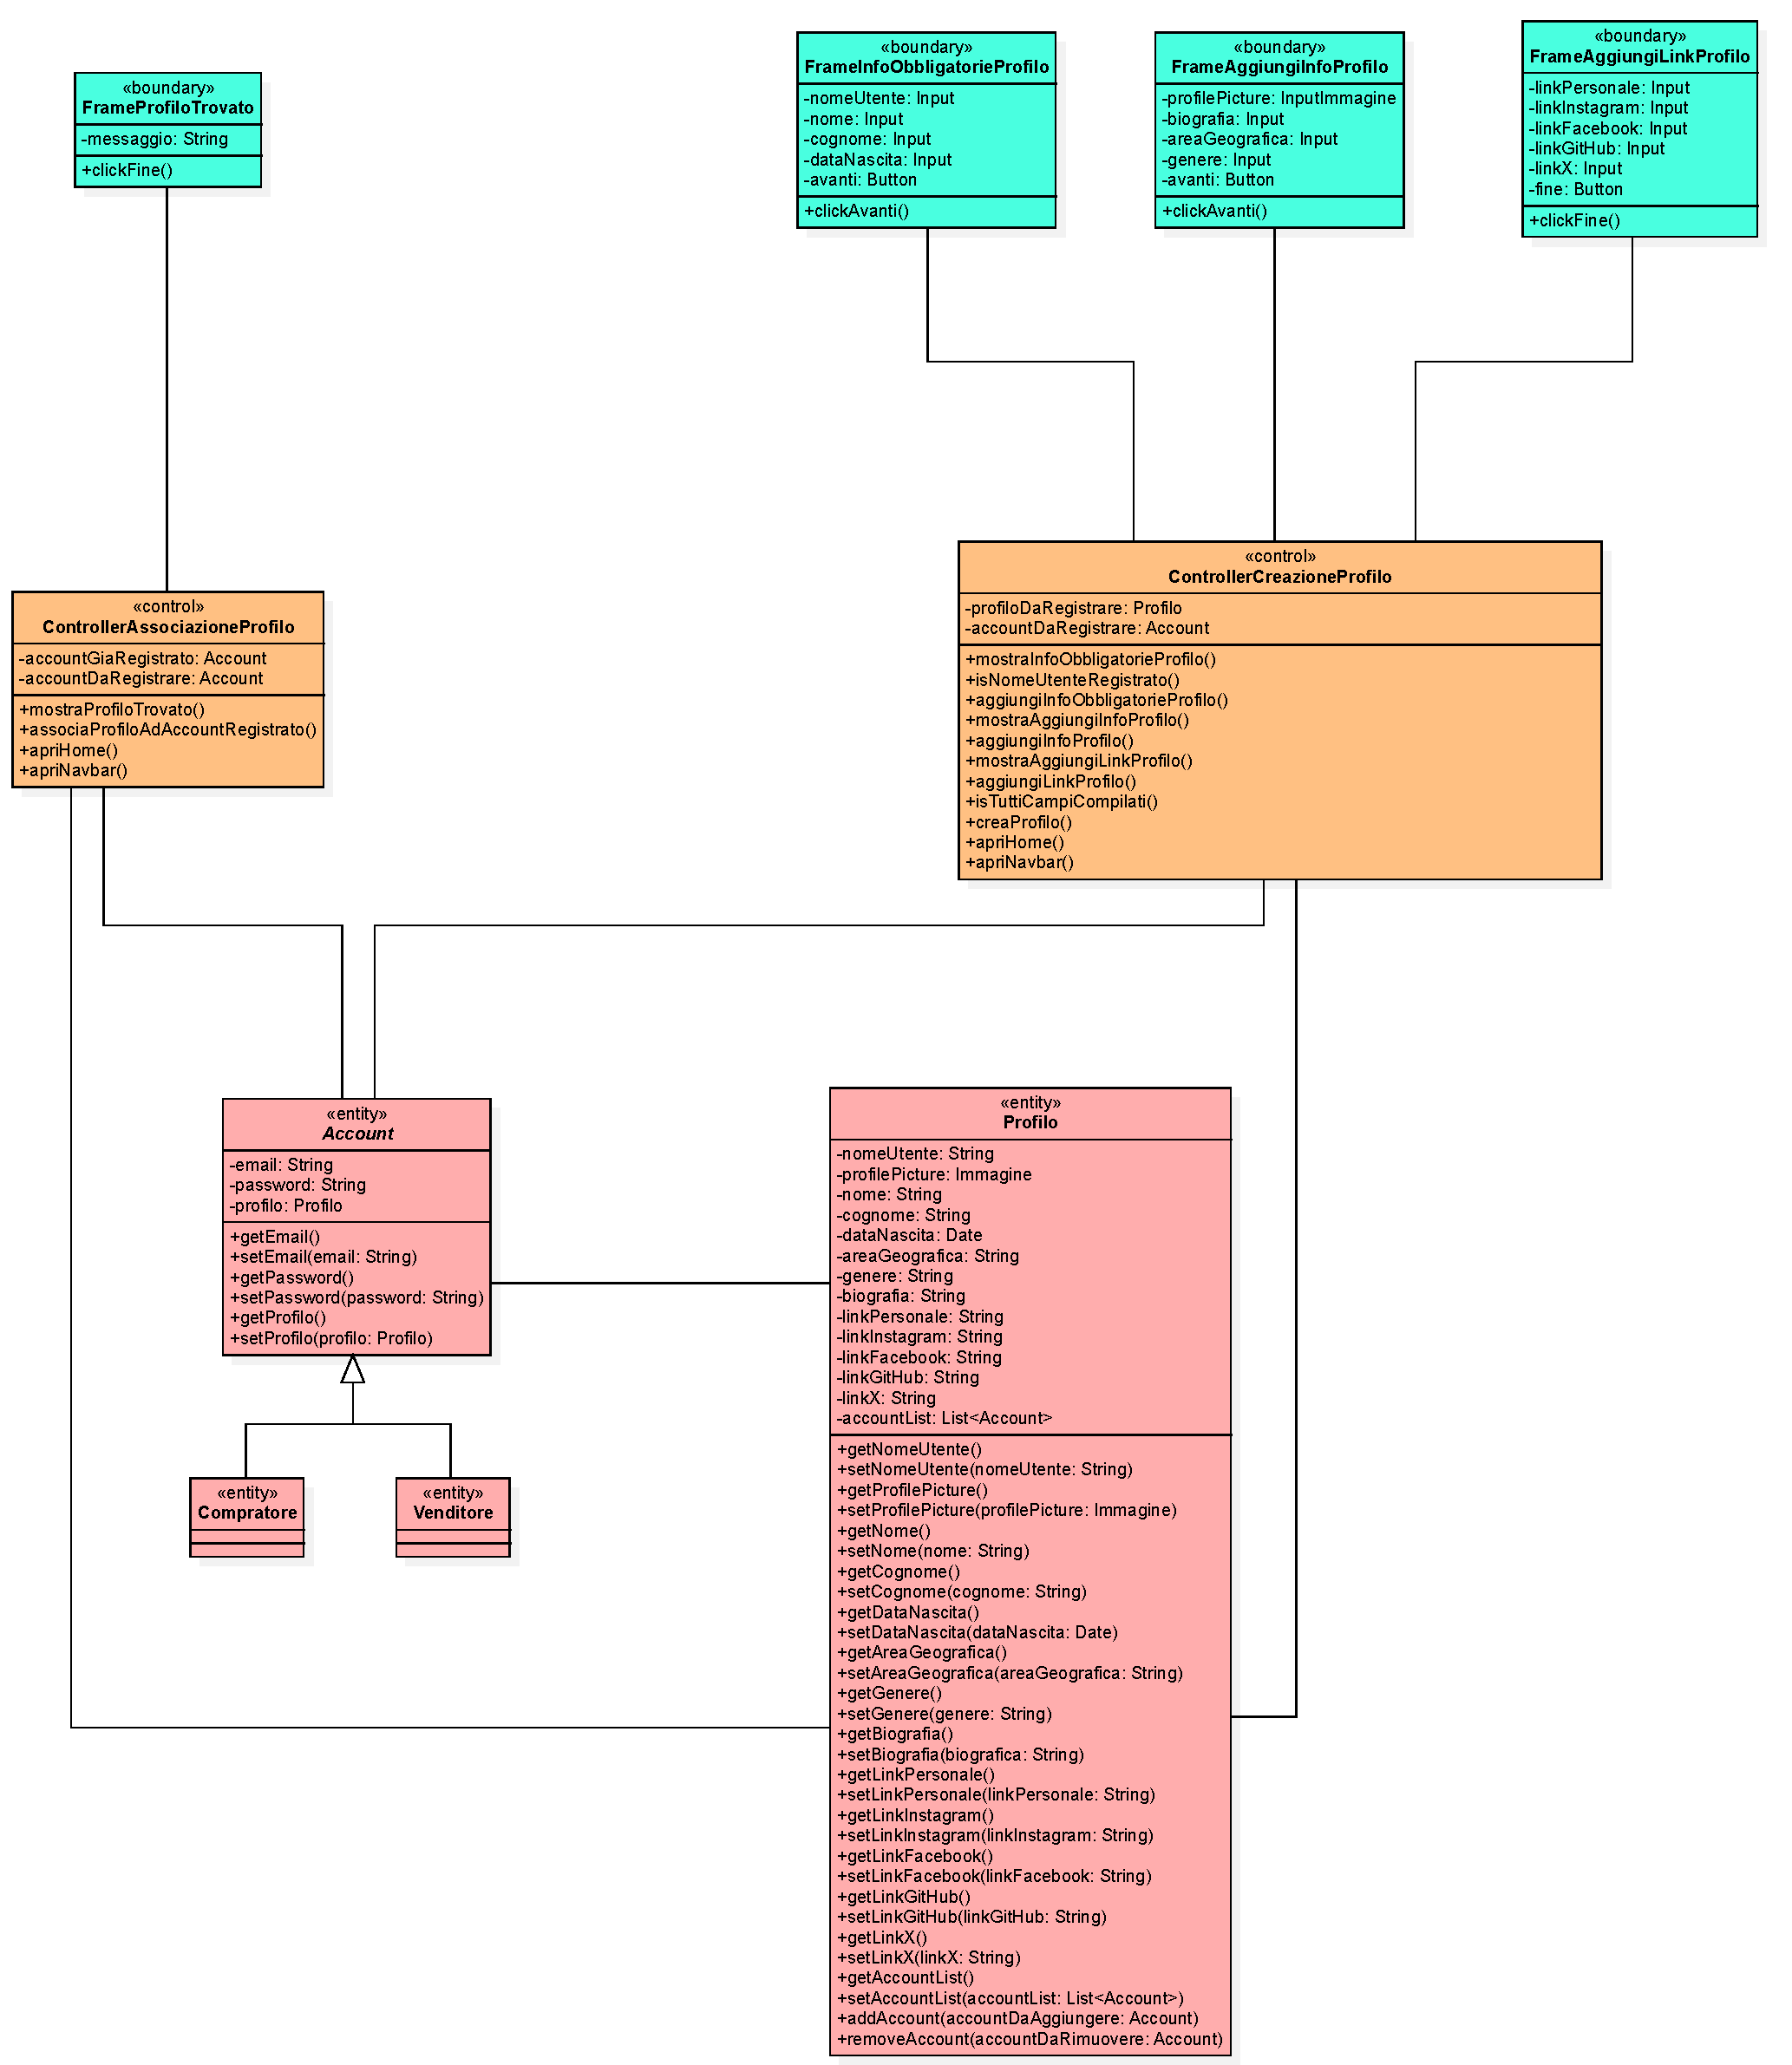
\includegraphics[width=1\linewidth]{Immagini/Diagrammi/Class Diagram/Utente che non ha effettuato l'accesso/CreazioneProfilo.pdf}
                \caption{Creazione del profilo}
            \end{figure}
            
            \begin{figure}[htbp!]
                \centering
                    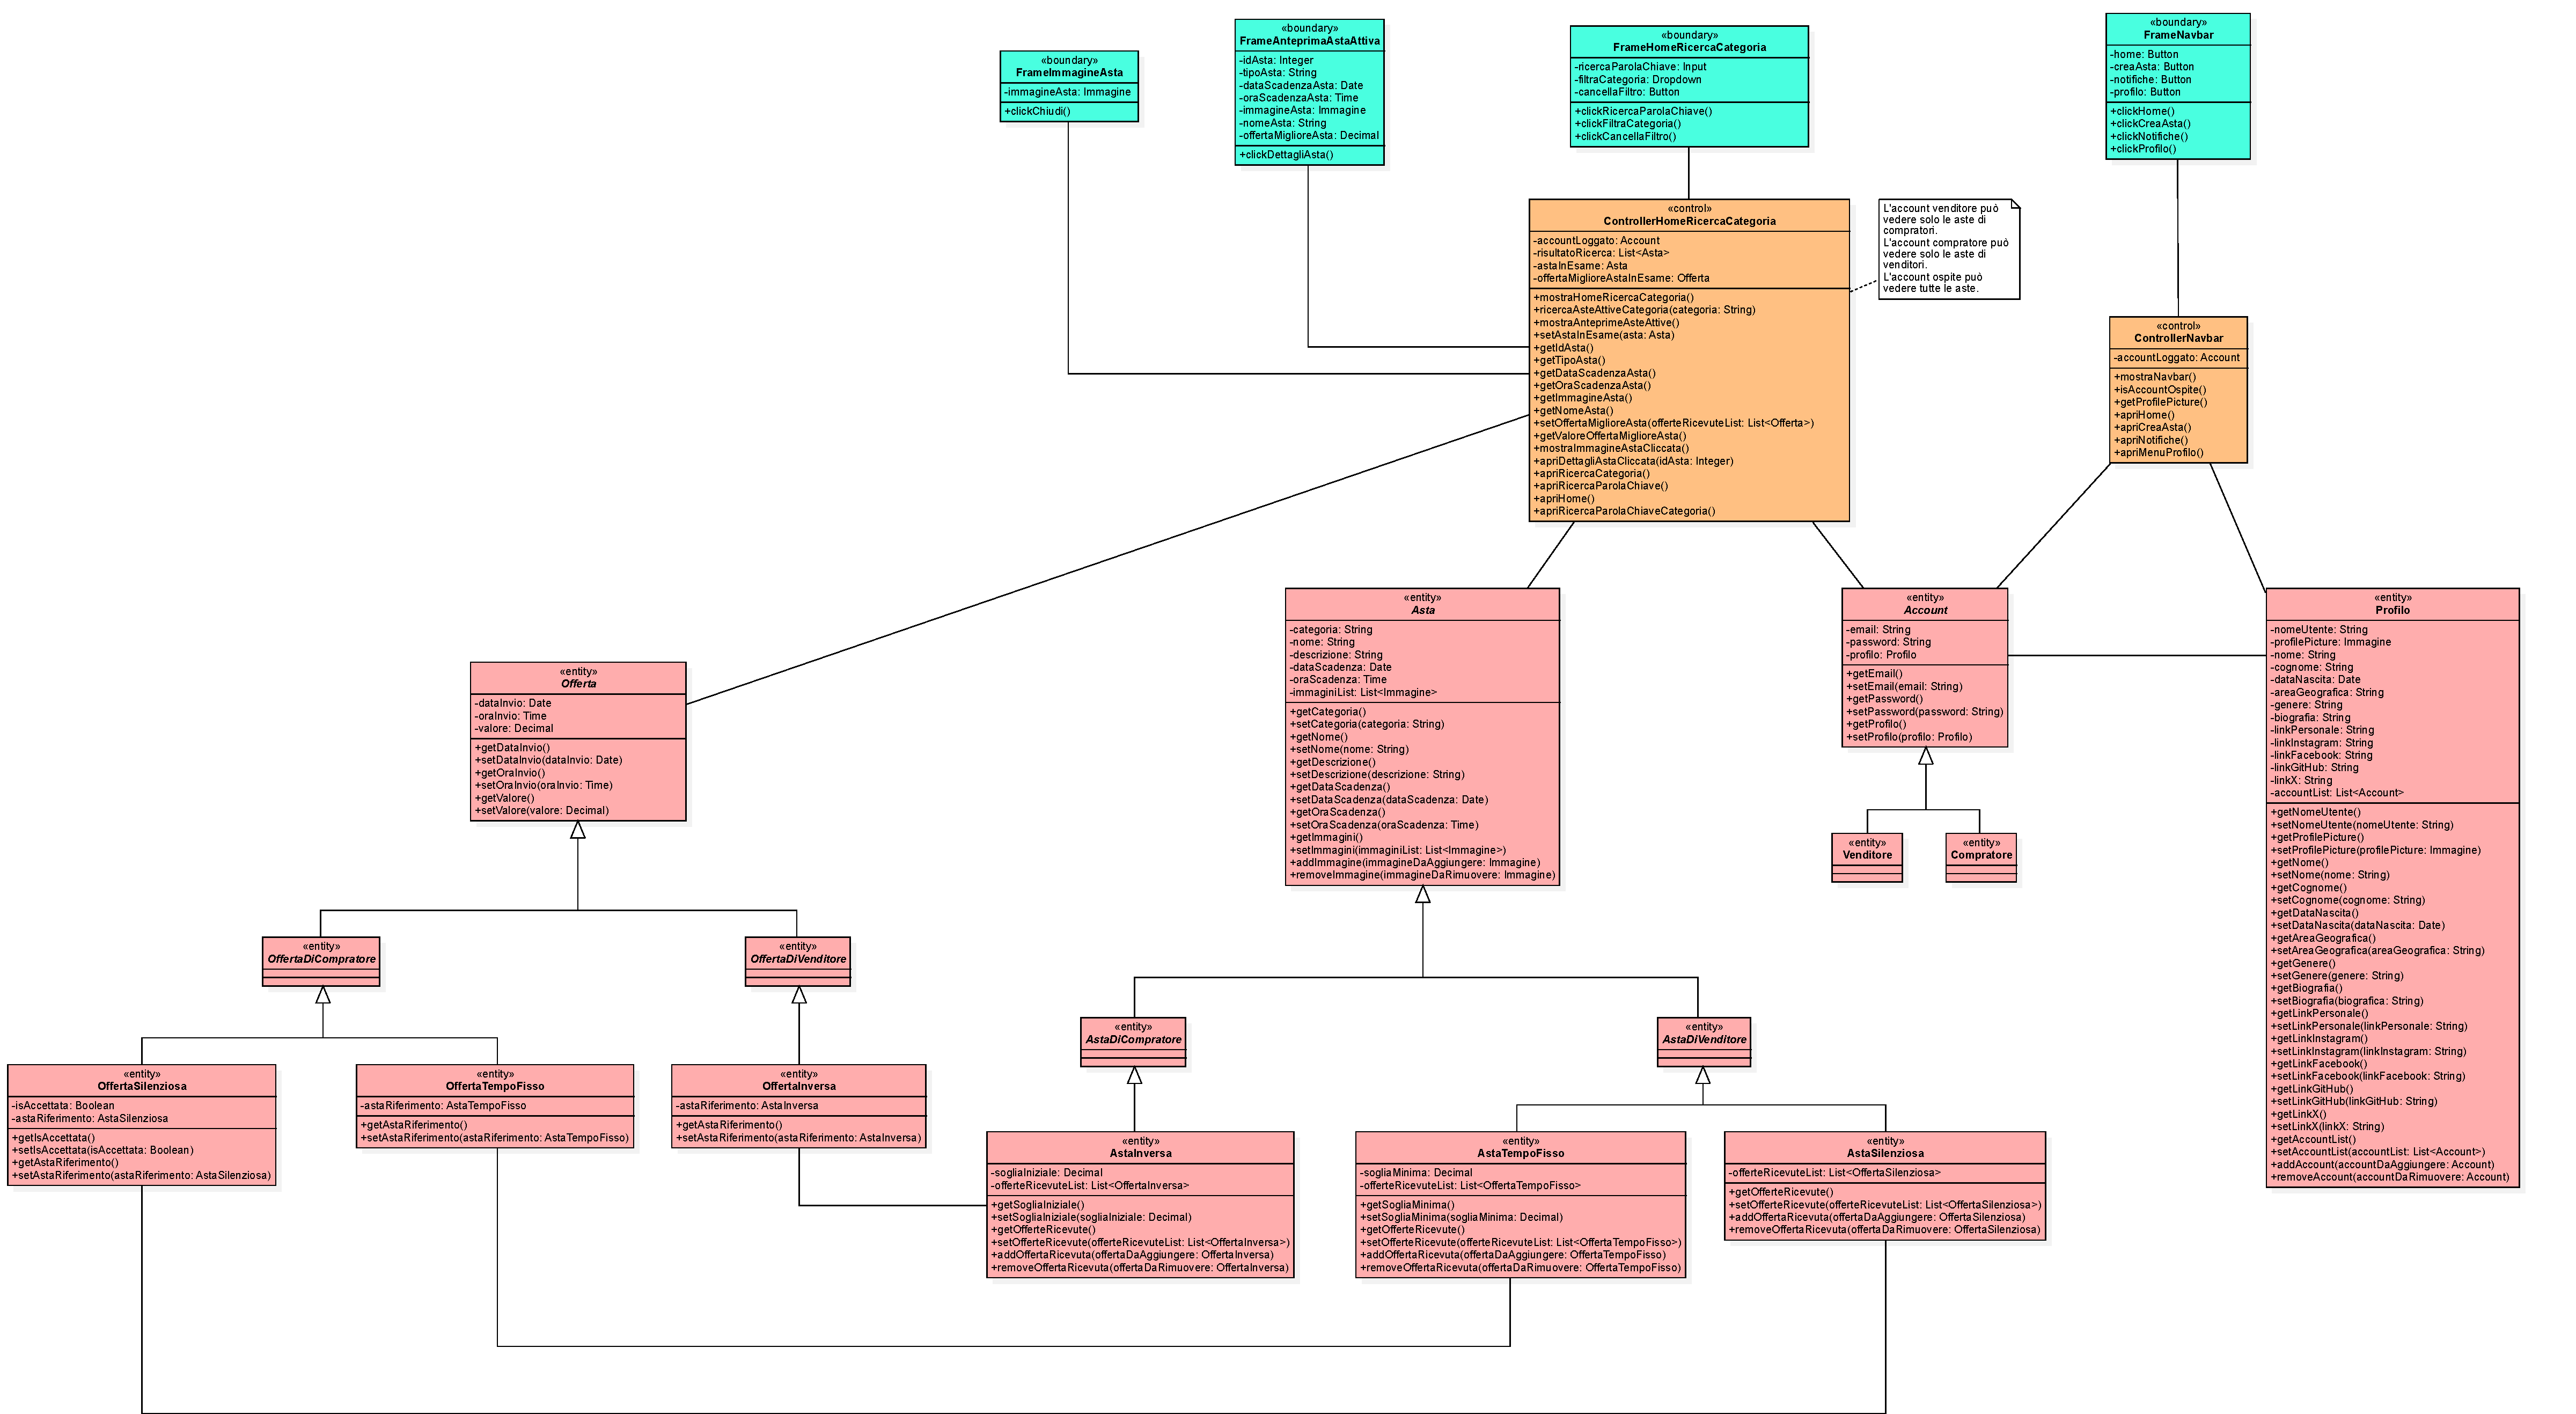
\includegraphics[width=1\linewidth]{Immagini/Diagrammi/Class Diagram/Utente generico/RicercaCategoria.pdf}
                \caption{Ricerca per categoria}
            \end{figure}
            
            \begin{figure}[htbp!]
                \centering
                    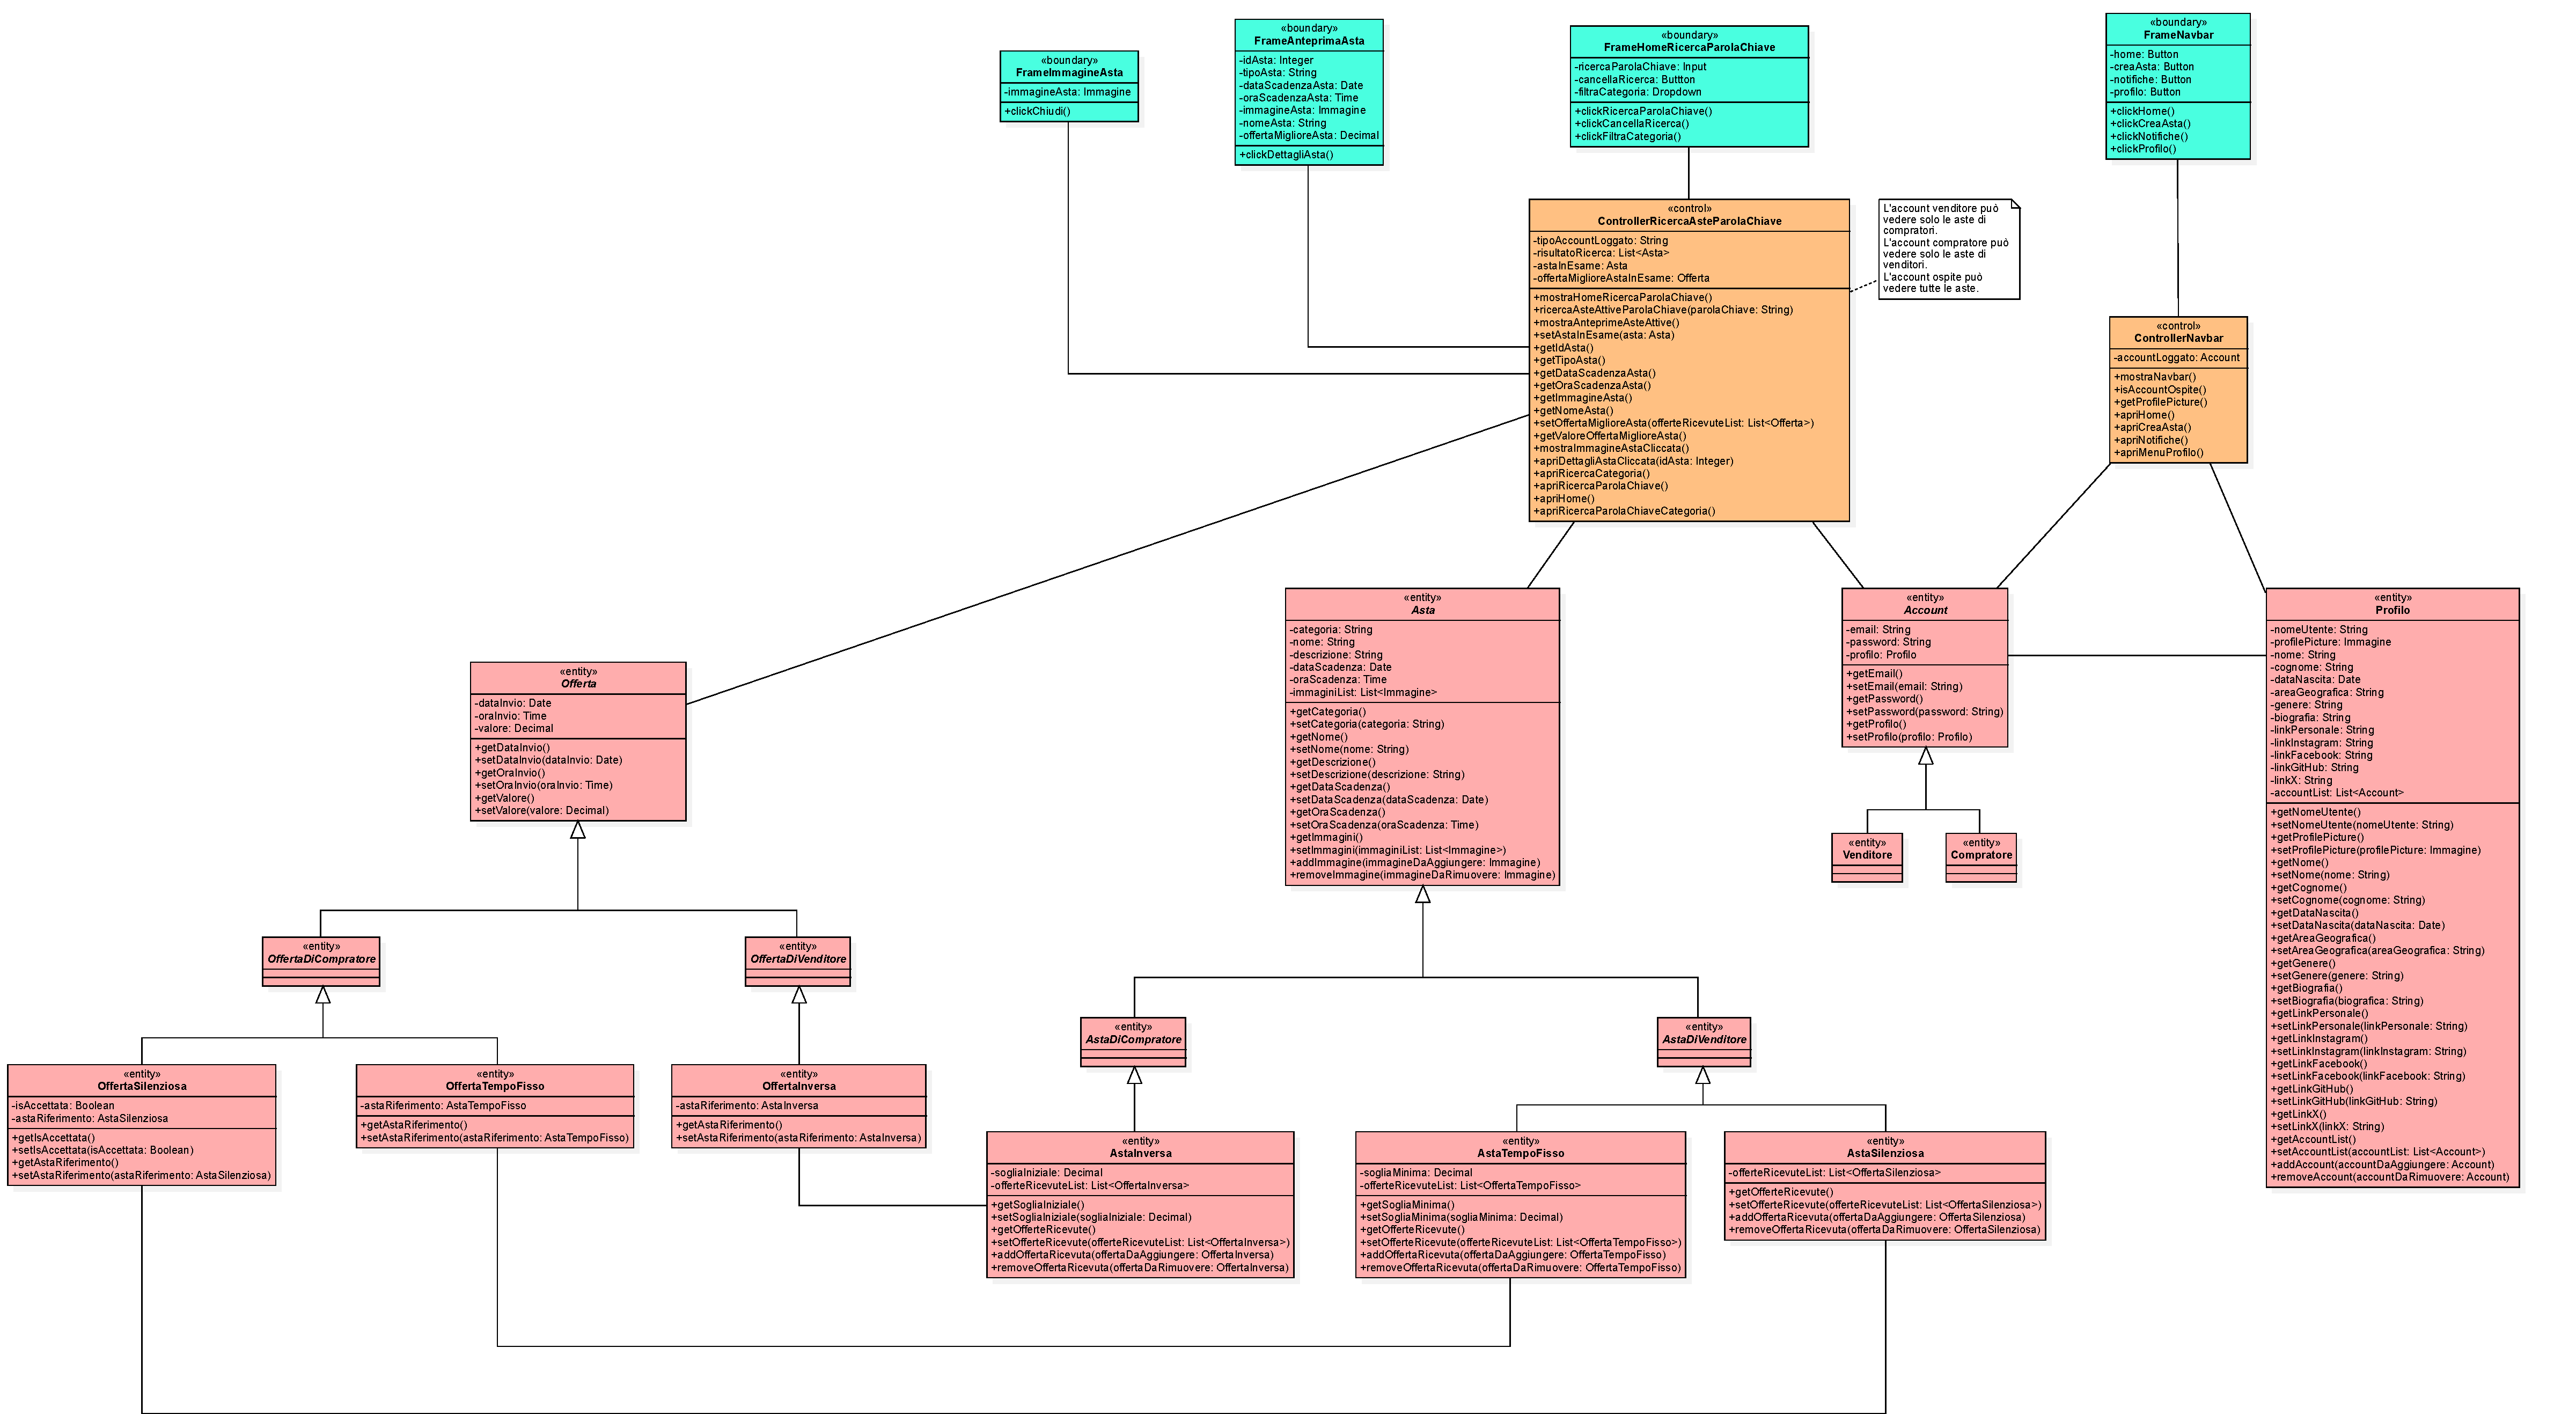
\includegraphics[width=1\linewidth]{Immagini/Diagrammi/Class Diagram/Utente generico/RicercaParolaChiave.pdf}
                \caption{Ricerca per parola chiave}
            \end{figure}
            
            \begin{figure}[htbp!]
                \centering
                    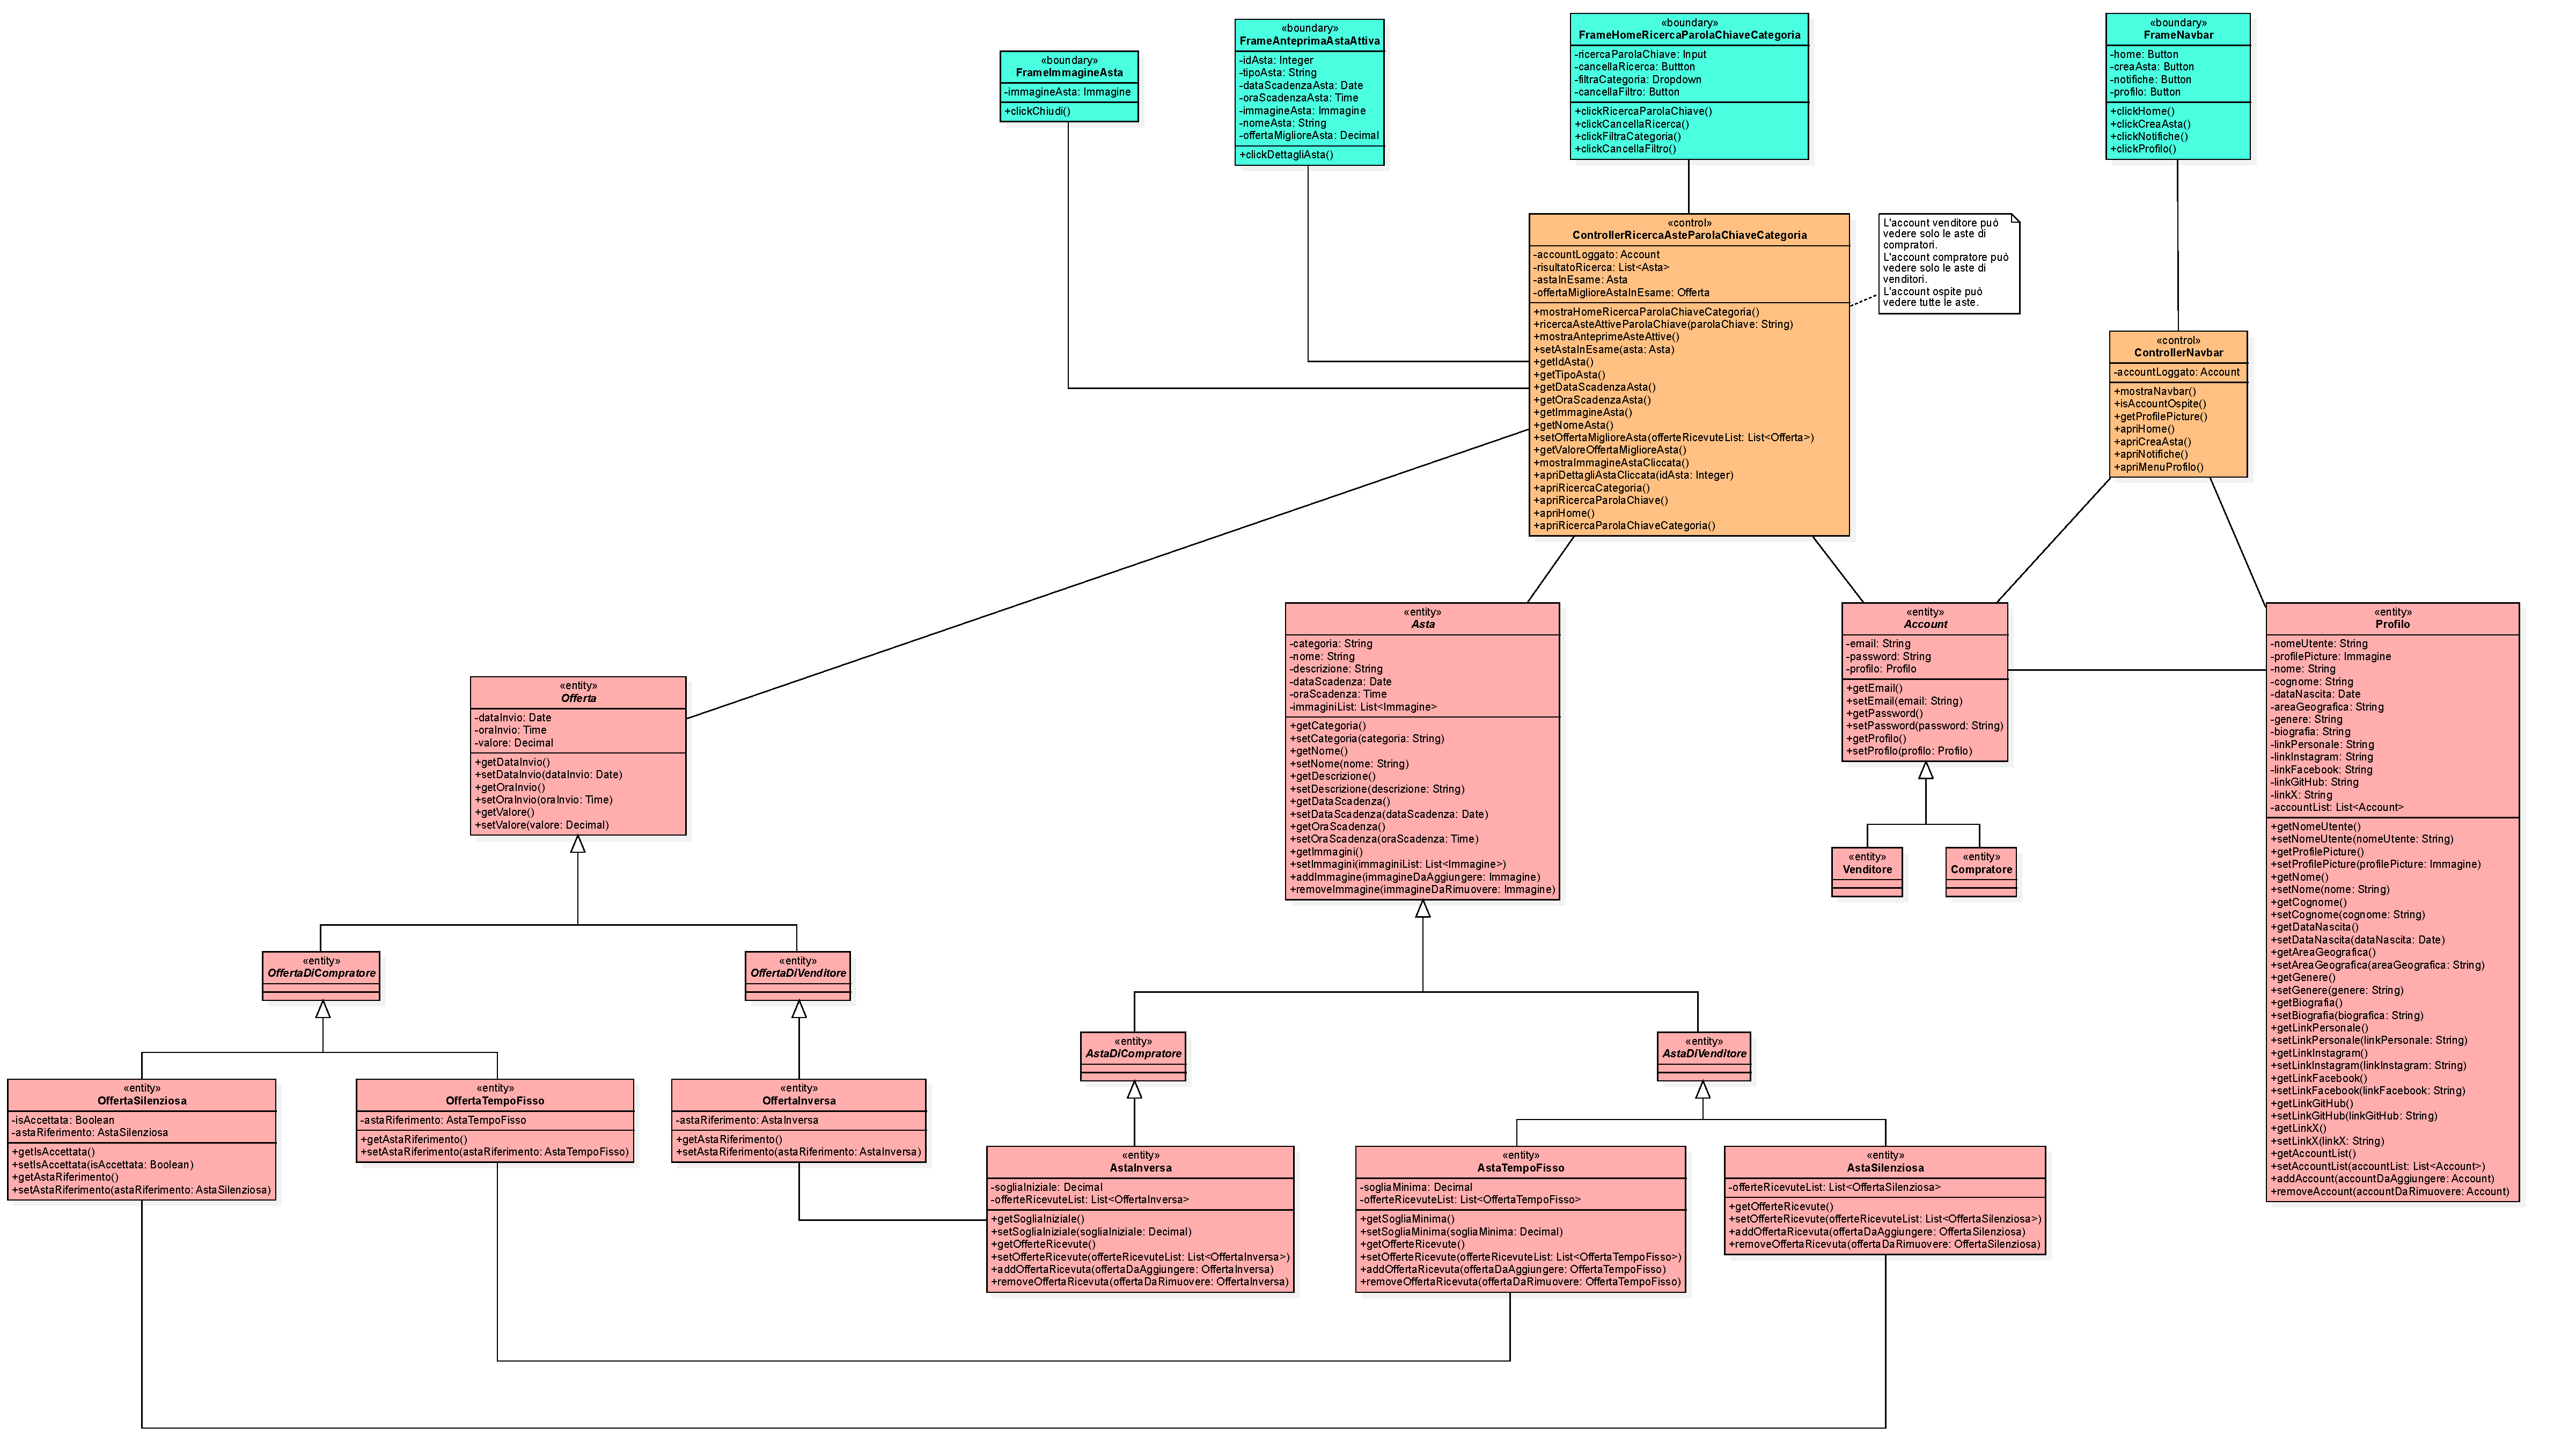
\includegraphics[width=1\linewidth]{Immagini/Diagrammi/Class Diagram/Utente generico/RicercaParolaChiaveCategoria.pdf}
                \caption{Ricerca per parola chiave e categoria}
            \end{figure}
            
            \begin{figure}[htbp!]
                \centering
                    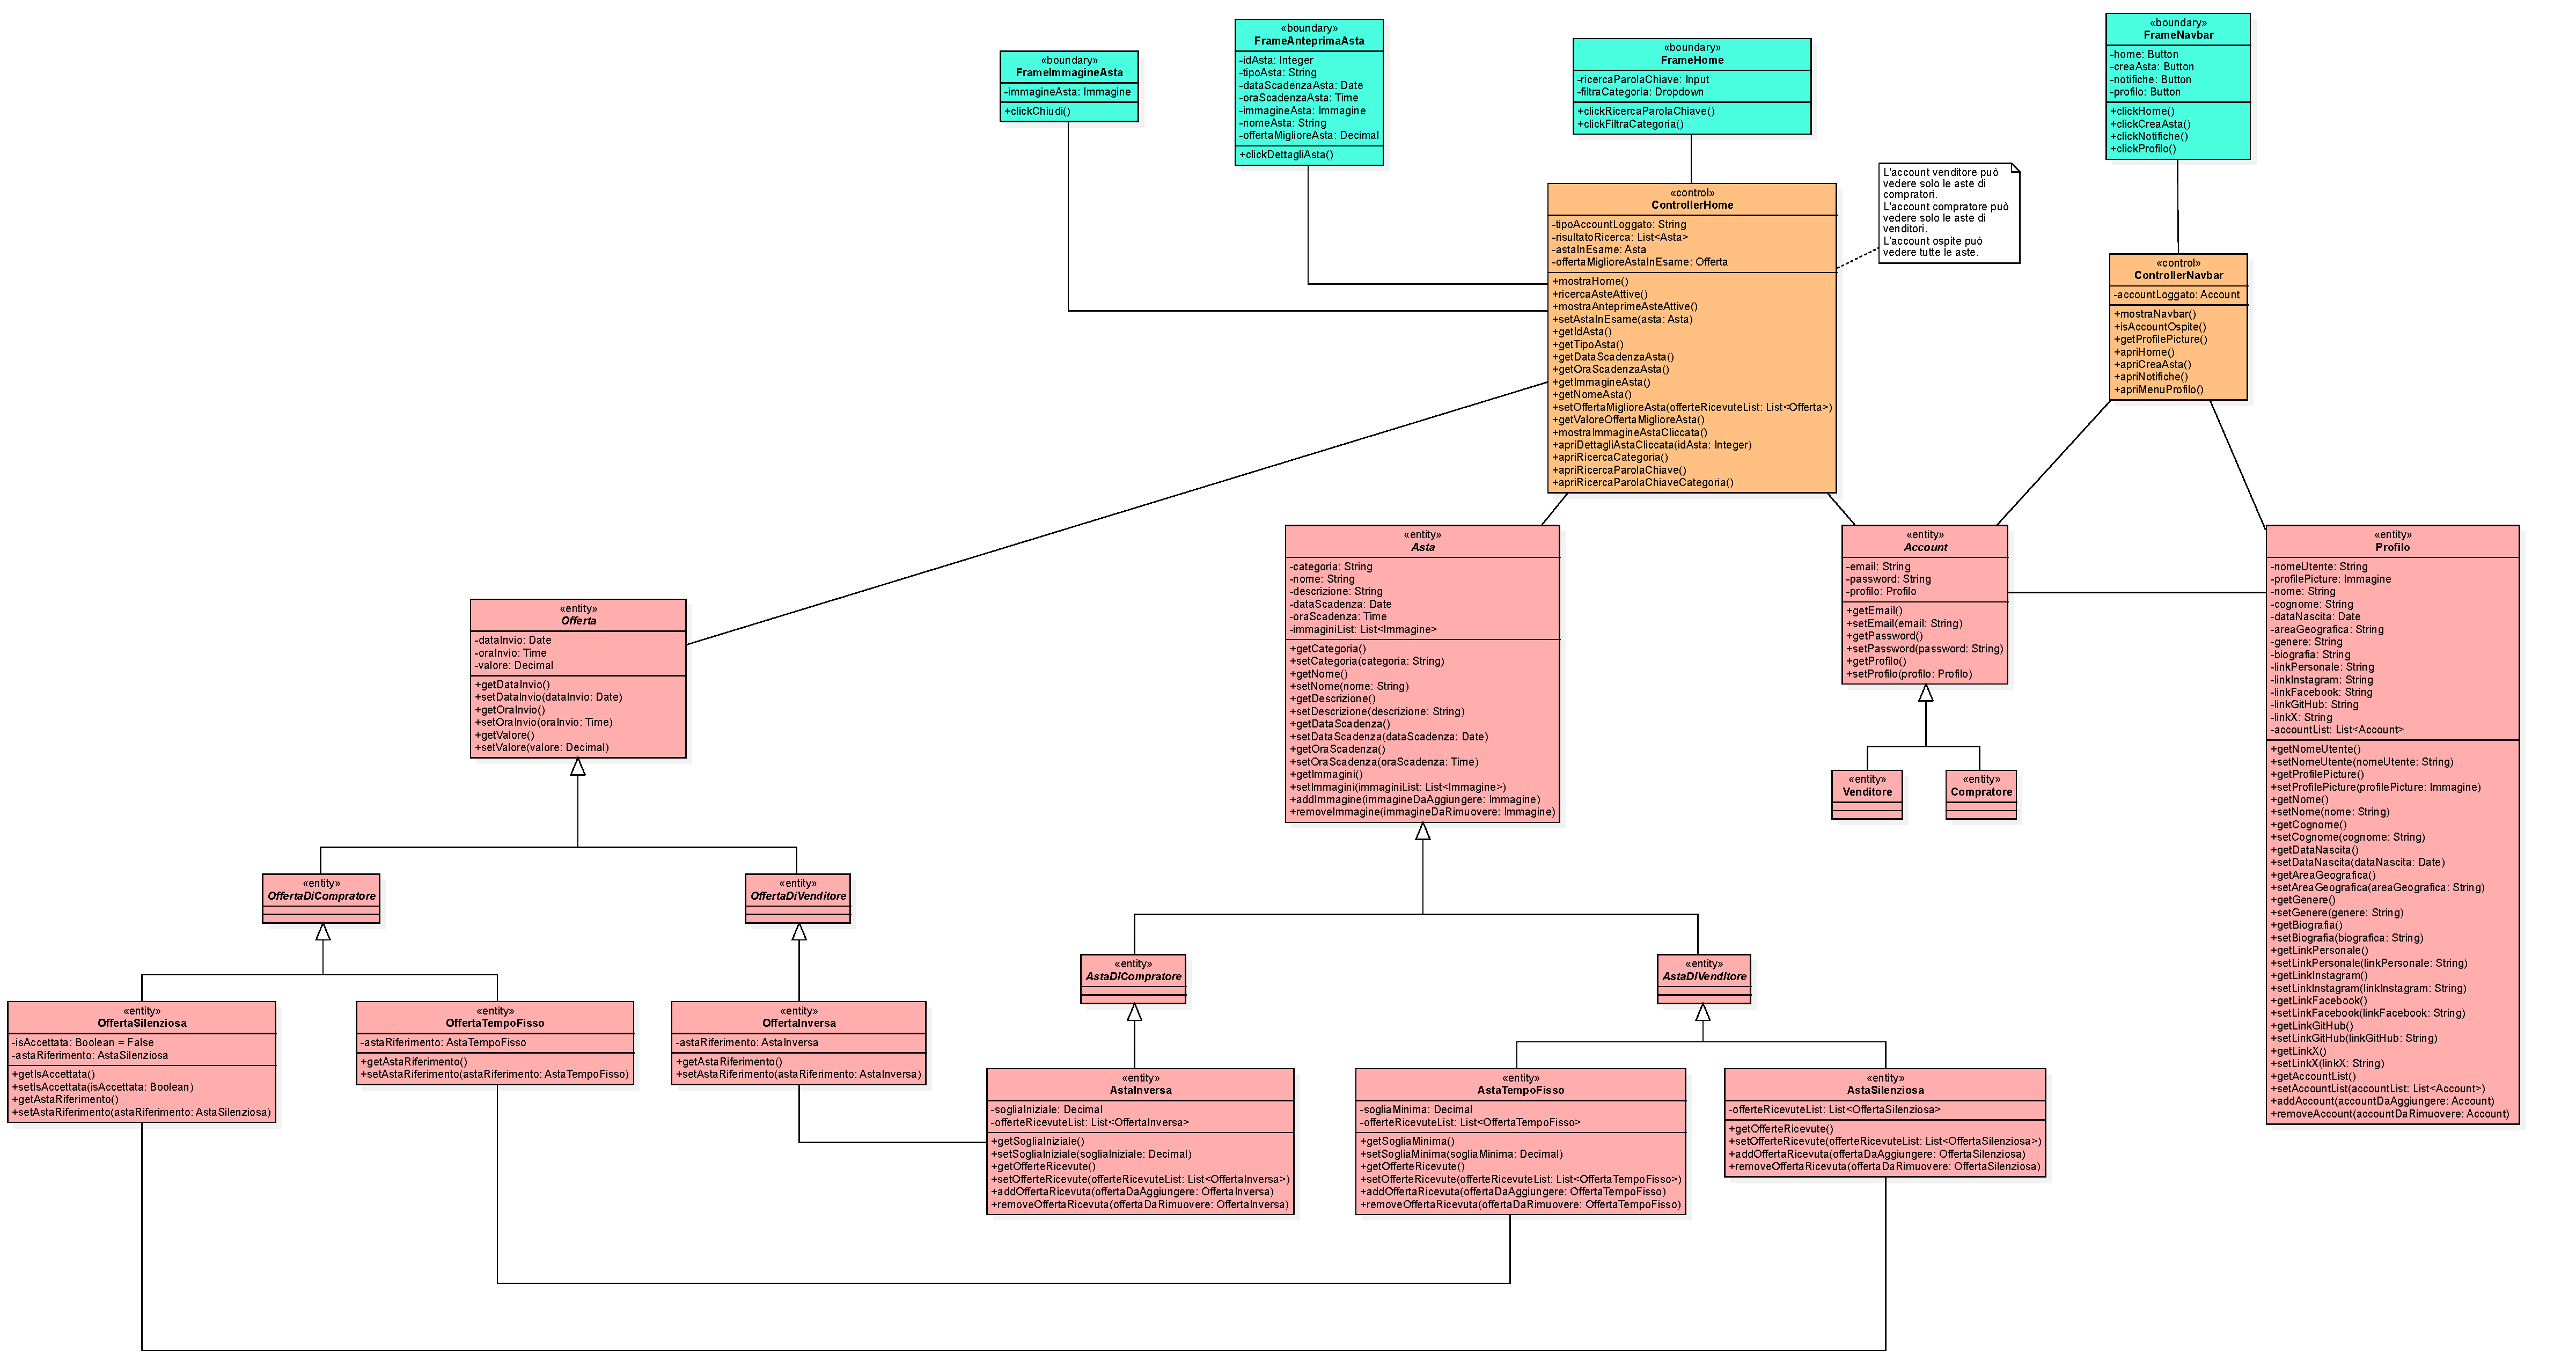
\includegraphics[width=1\linewidth]{Immagini/Diagrammi/Class Diagram/Utente generico/VisualizzaAsteAttive.pdf}
                \caption{Visualizza aste attive}
            \end{figure}
            
            \begin{figure}[htbp!]
                \centering
                    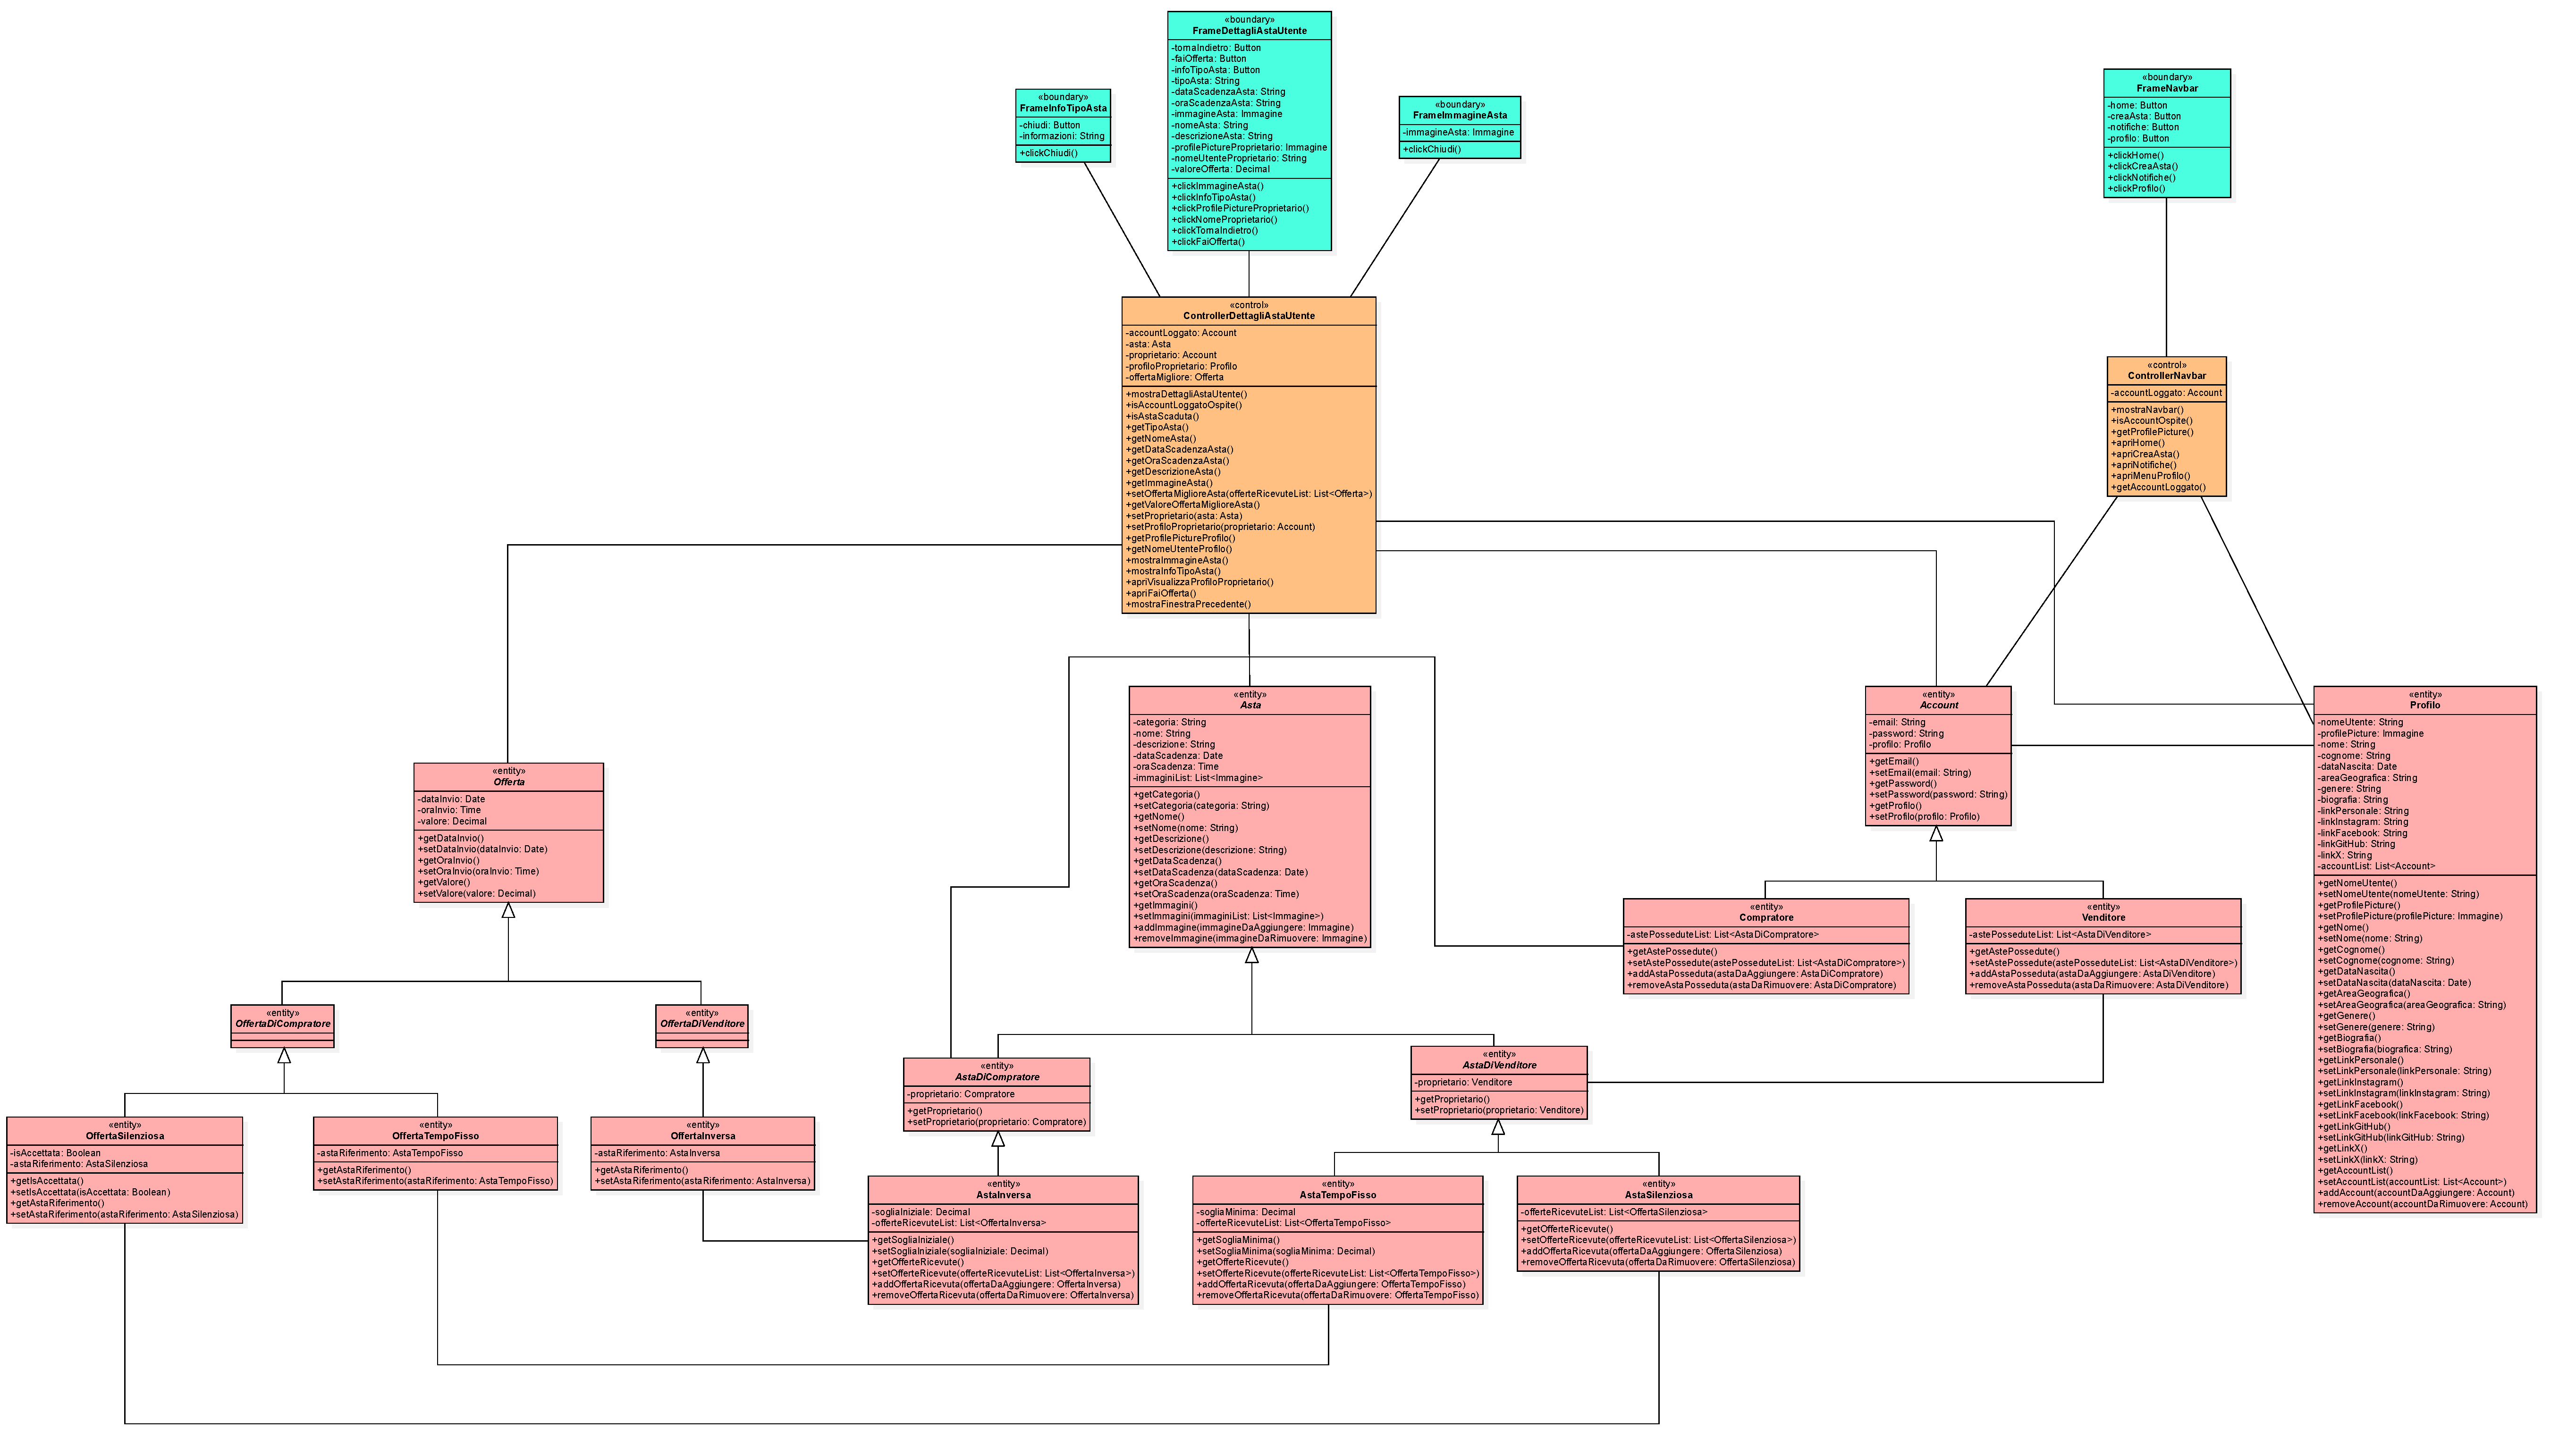
\includegraphics[width=1\linewidth]{Immagini/Diagrammi/Class Diagram/Utente generico/VisualizzaDettagliAstaUtente.pdf}
                \caption{Visualizza dettagli asta di un altro utente}
            \end{figure}
            
            \begin{figure}[htbp!]
                \centering
                    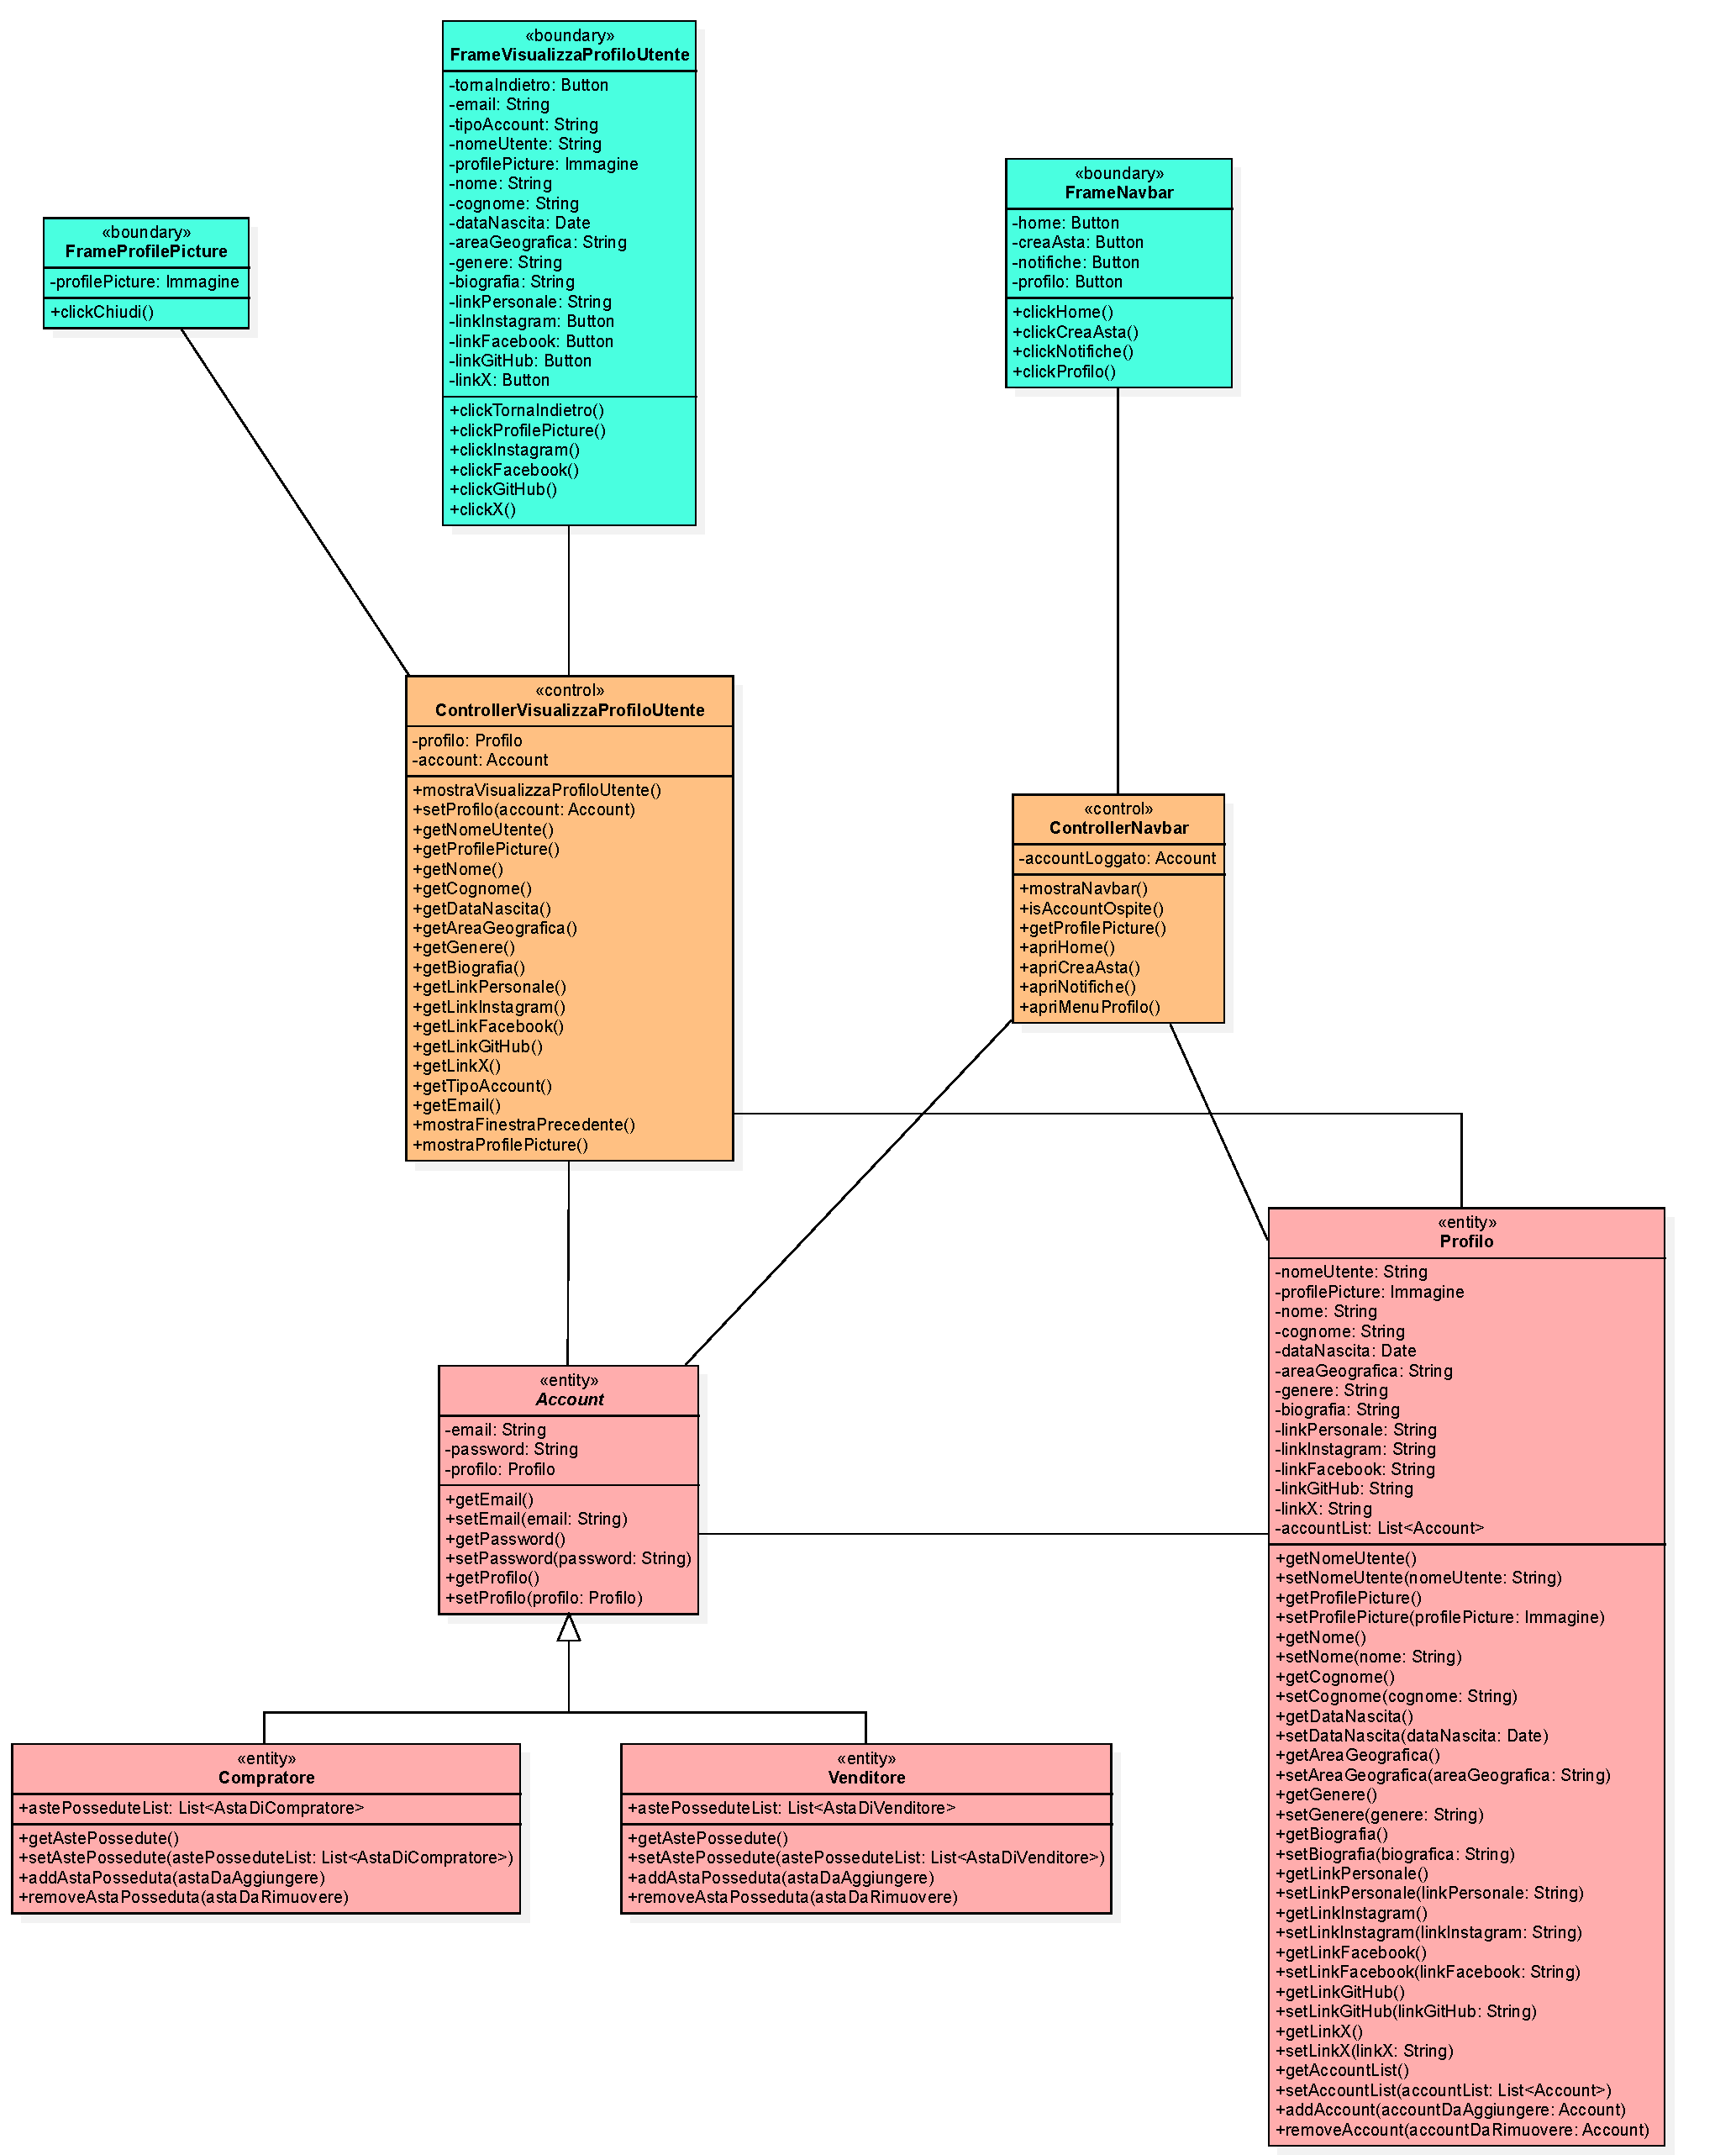
\includegraphics[width=1\linewidth]{Immagini/Diagrammi/Class Diagram/Utente generico/VisualizzaProfiloUtente.pdf}
                \caption{Visualizza profilo utente}
            \end{figure}
            
            \begin{figure}[htbp!]
                \centering
                    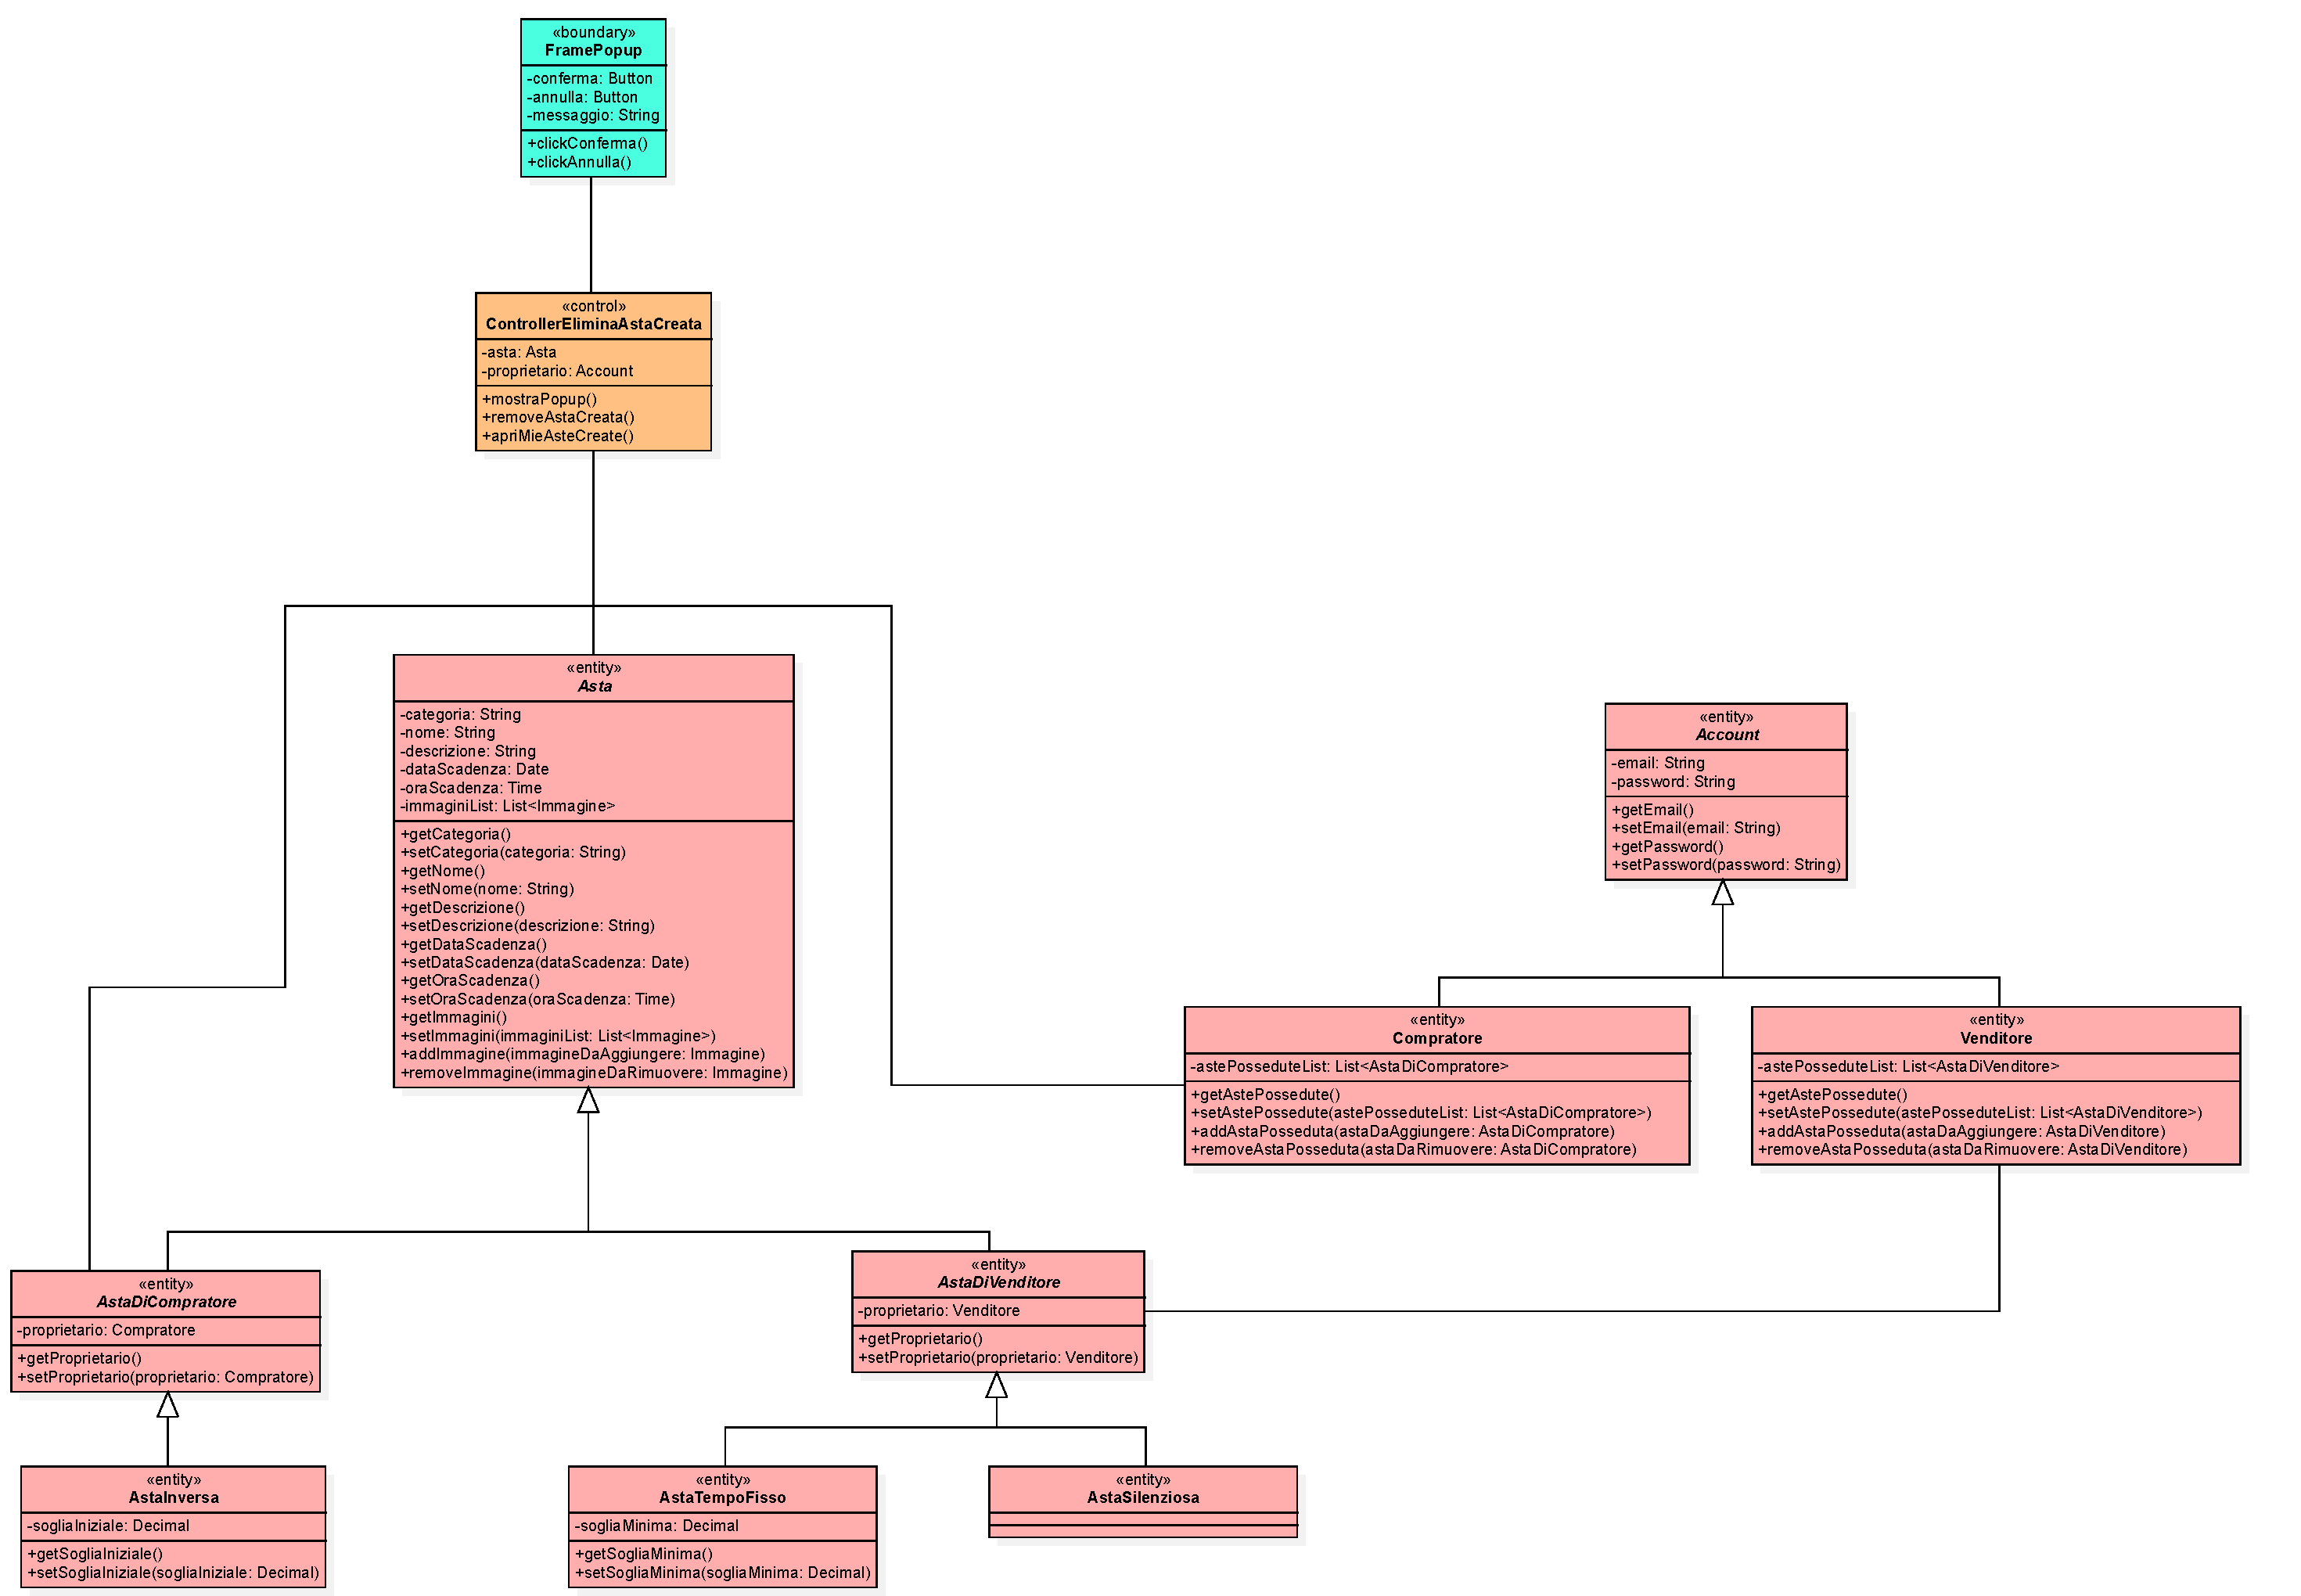
\includegraphics[width=1\linewidth]{Immagini/Diagrammi/Class Diagram/Utente che ha effettuato l'accesso/EliminaAsta.pdf}
                \caption{Elimina asta creata}
            \end{figure}
            
            \begin{figure}[htbp!]
                \centering
                    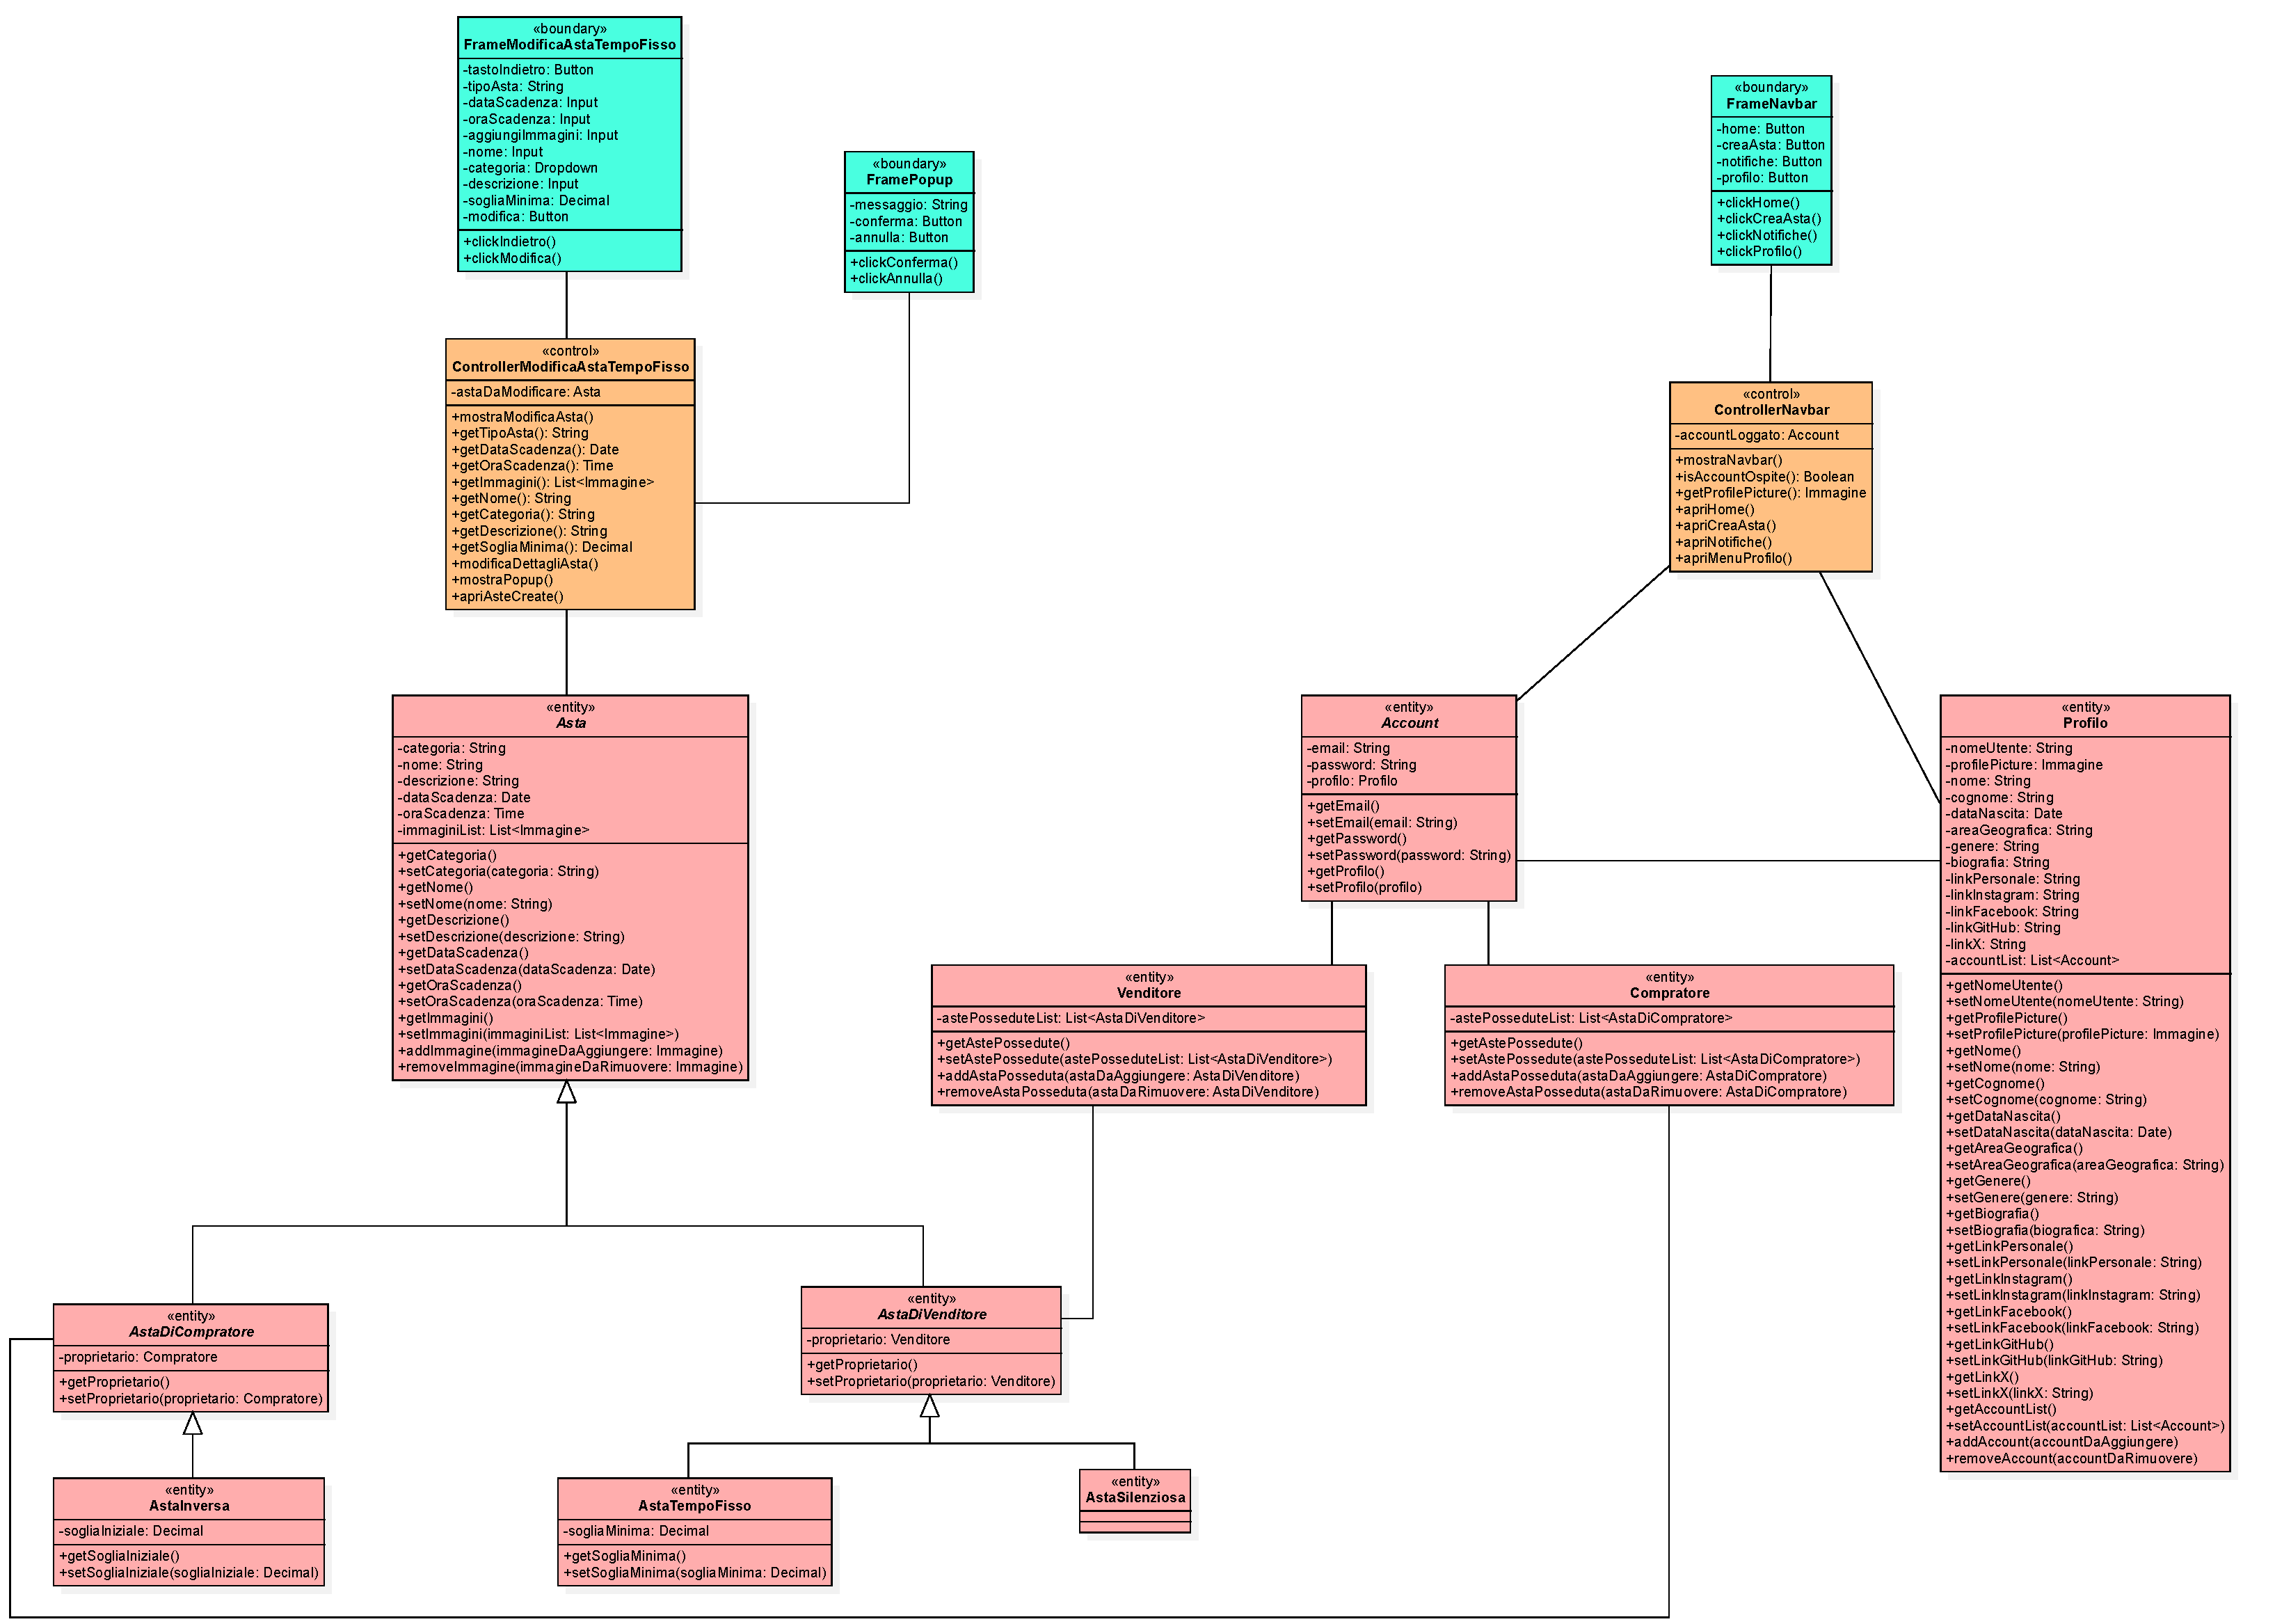
\includegraphics[width=1\linewidth]{Immagini/Diagrammi/Class Diagram/Utente che ha effettuato l'accesso/ModificaAstaTempoFisso.pdf}
                \caption{Modifica asta a tempo fisso}
            \end{figure}
            
            \begin{figure}[htbp!]
                \centering
                    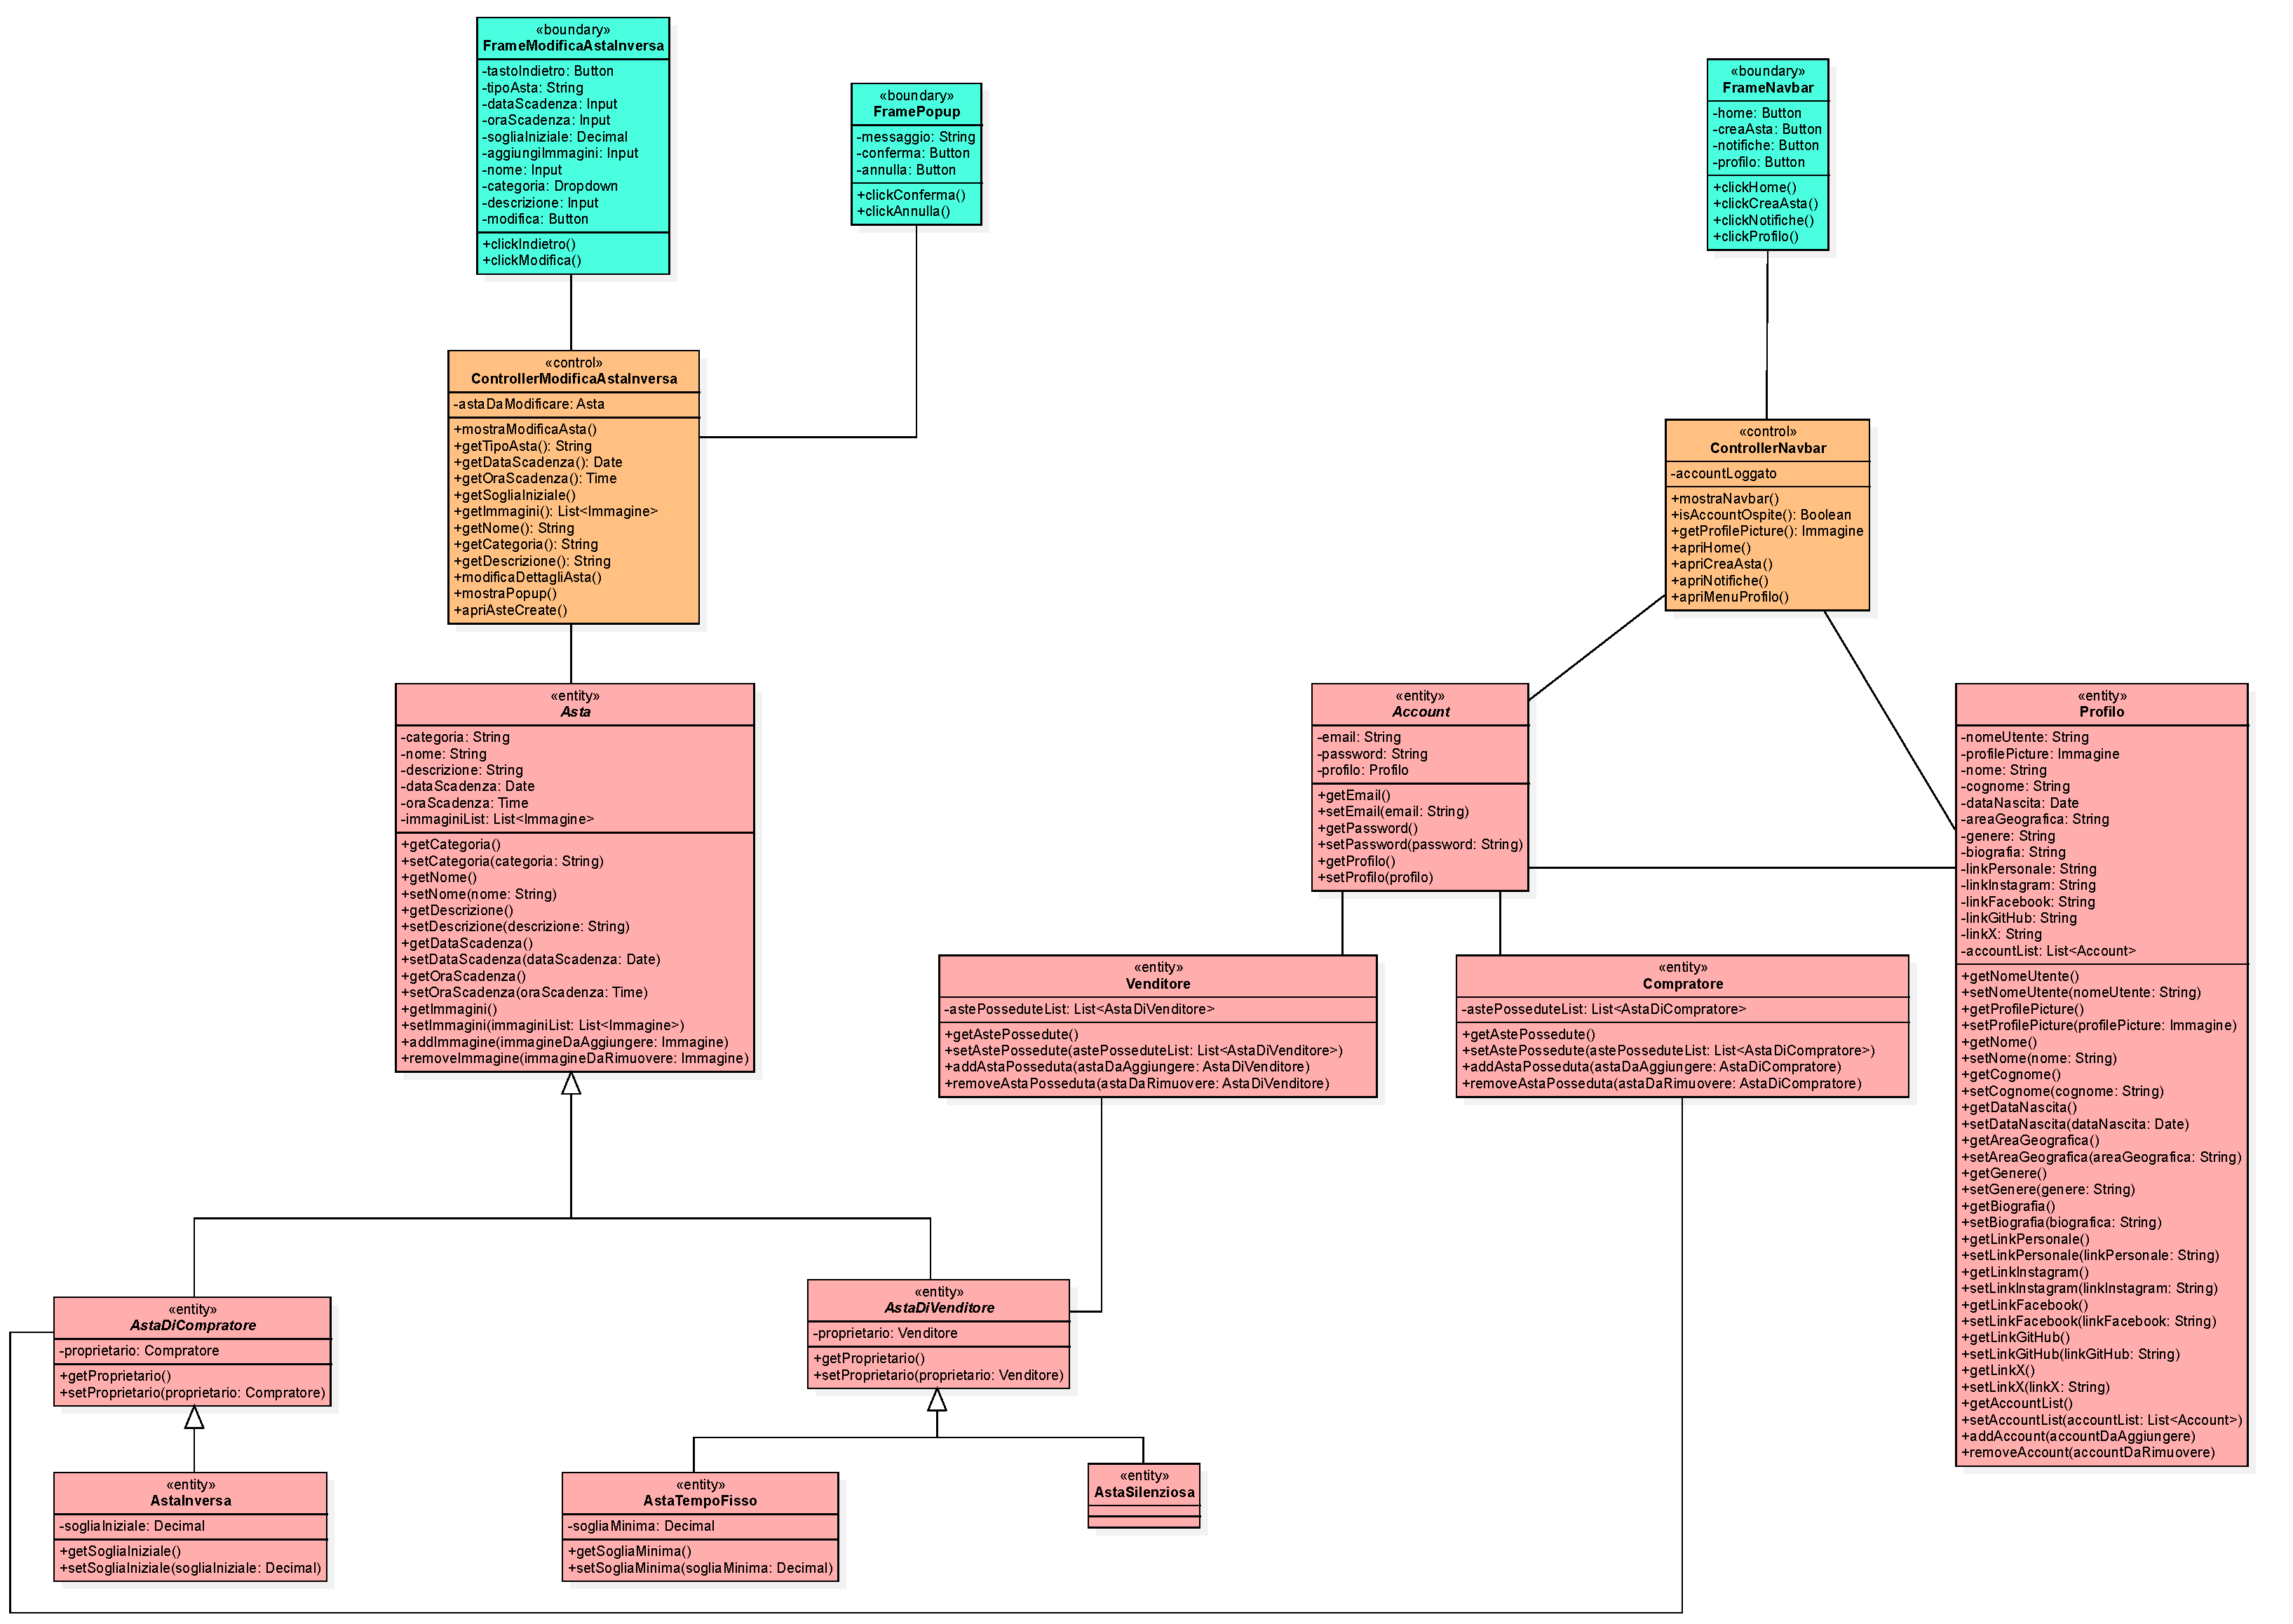
\includegraphics[width=1\linewidth]{Immagini/Diagrammi/Class Diagram/Utente che ha effettuato l'accesso/ModificaAstaInversa.pdf}
                \caption{Modifica asta inversa}
            \end{figure}
            
            \begin{figure}[htbp!]
                \centering
                    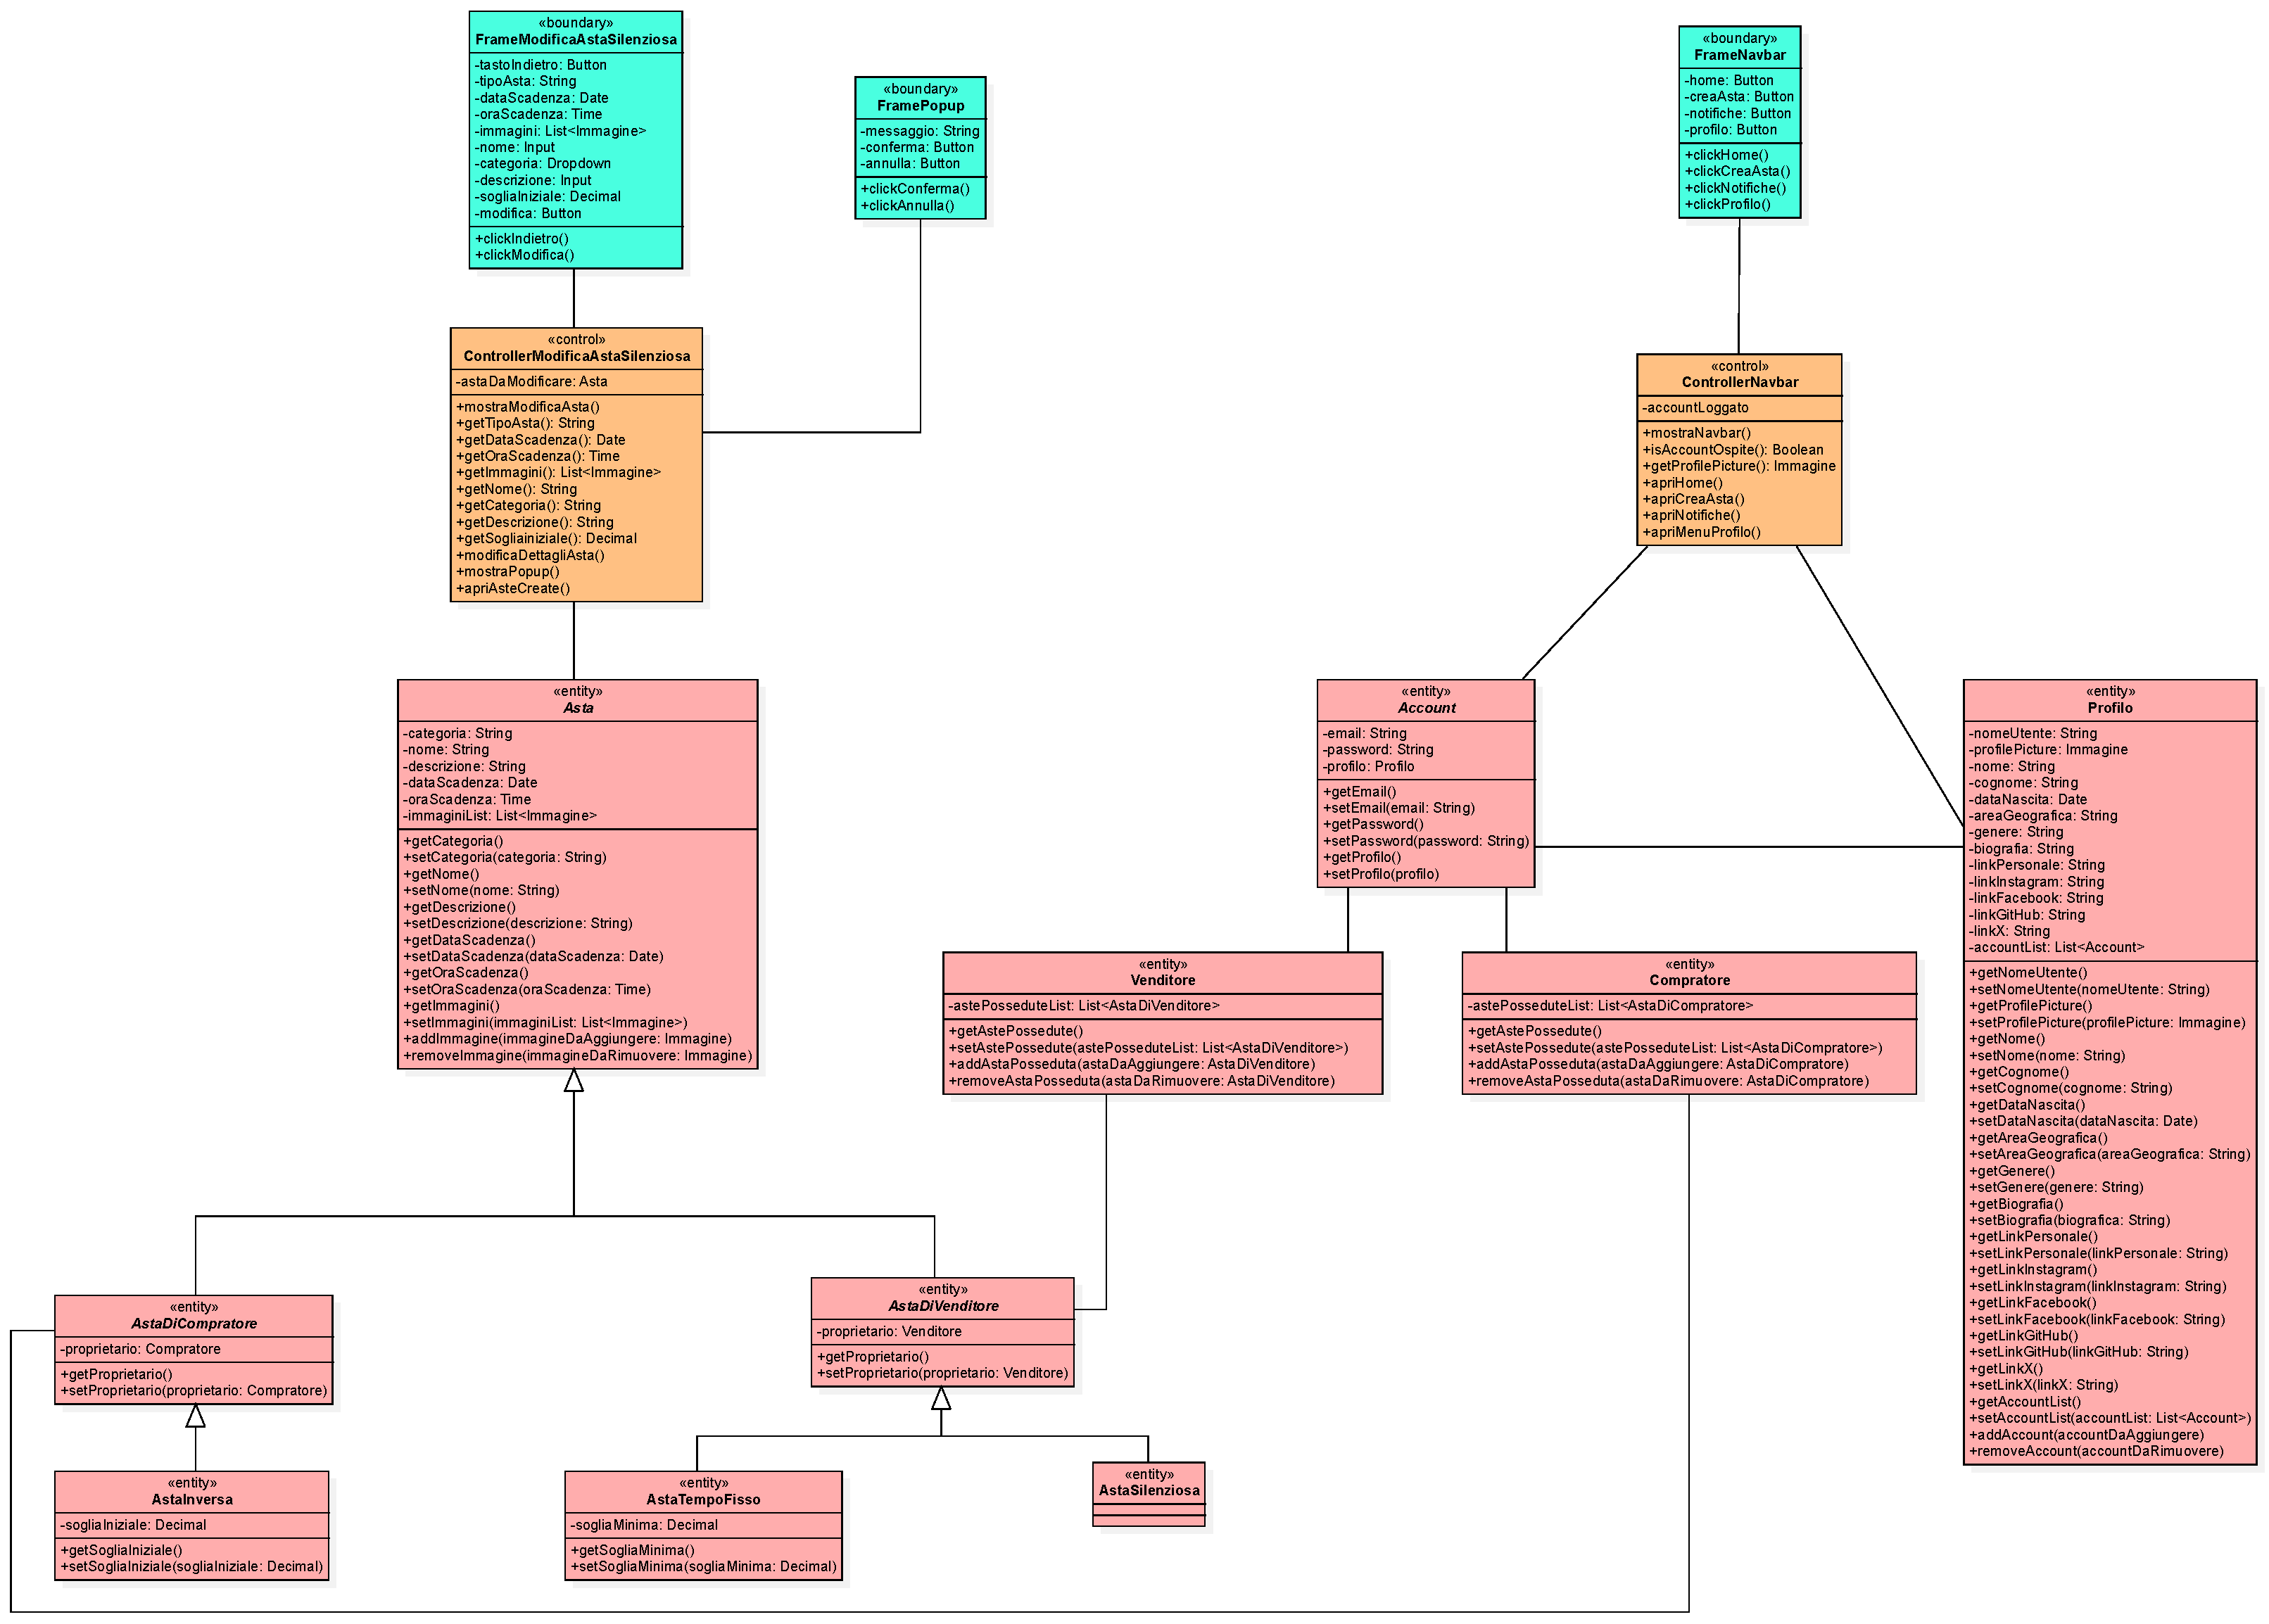
\includegraphics[width=1\linewidth]{Immagini/Diagrammi/Class Diagram/Utente che ha effettuato l'accesso/ModificaAstaSilenziosa.pdf}
                \caption{Modifica asta silenziosa}
            \end{figure}
            
            \begin{figure}[htbp!]
                \centering
                    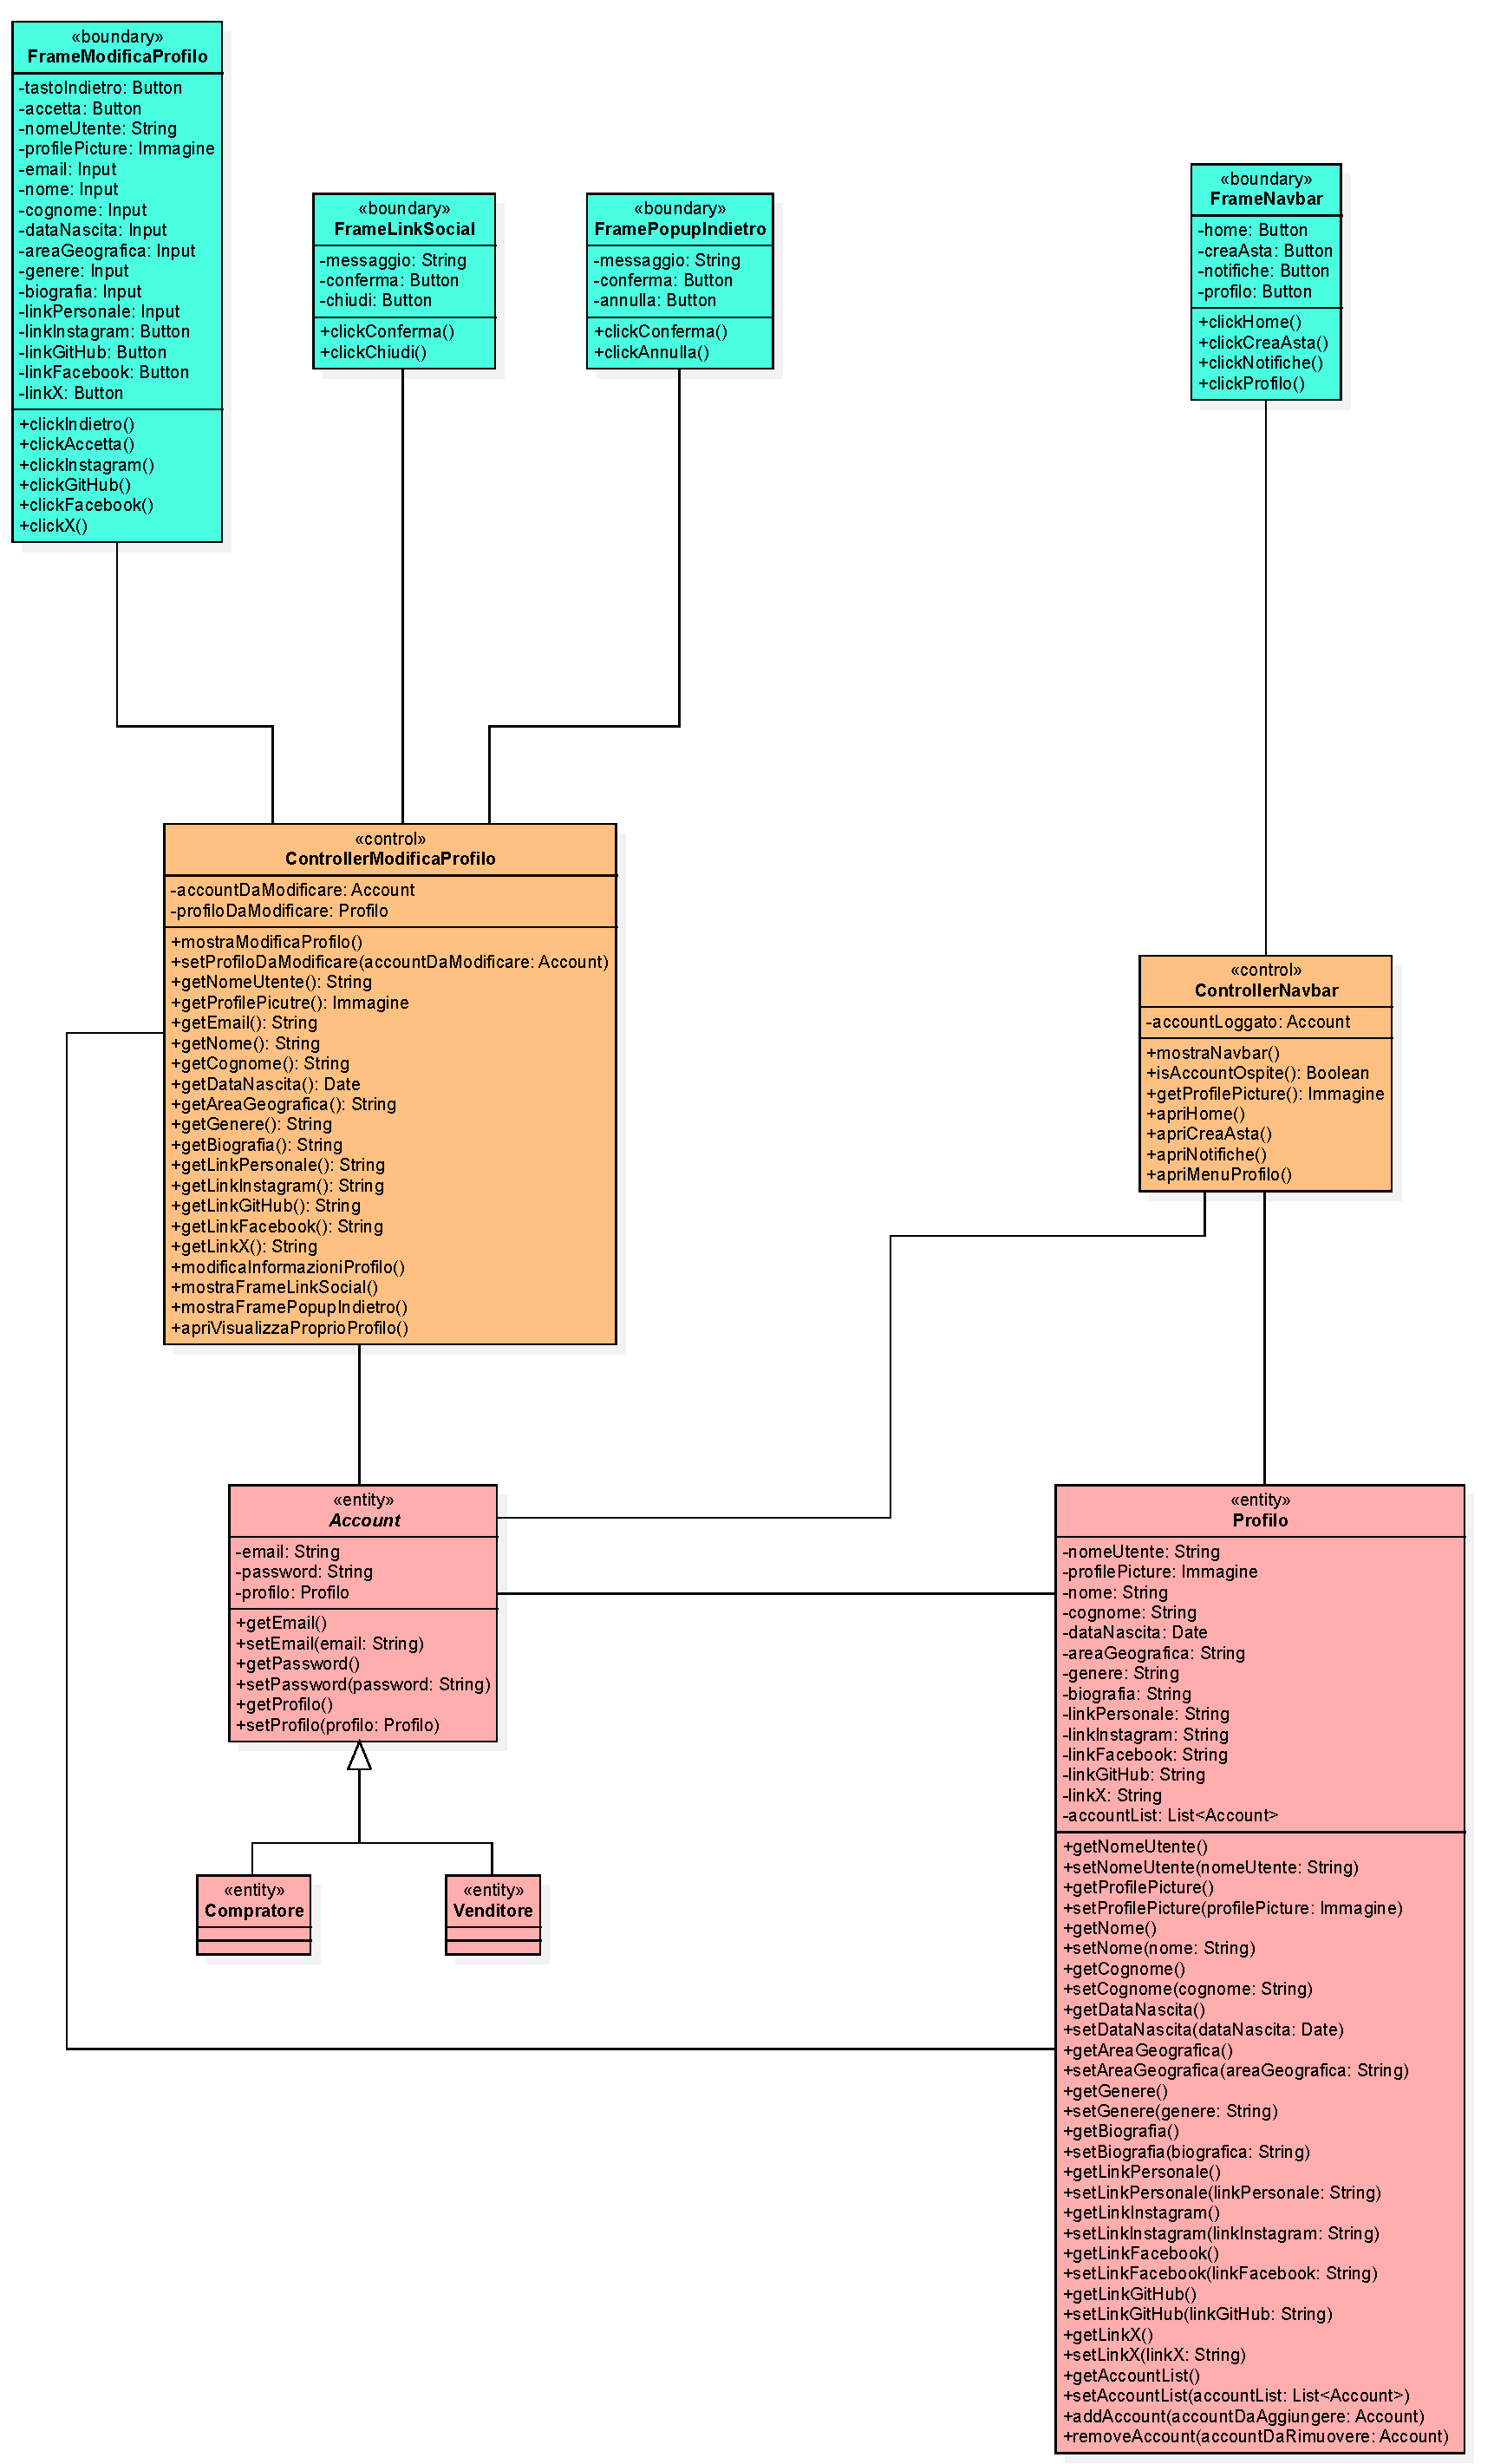
\includegraphics[width=0.8\linewidth]{Immagini/Diagrammi/Class Diagram/Utente che ha effettuato l'accesso/ModificaProfilo.pdf}
                \caption{Modifica profilo}
            \end{figure}

            \begin{figure}[htbp!]
                \centering
                    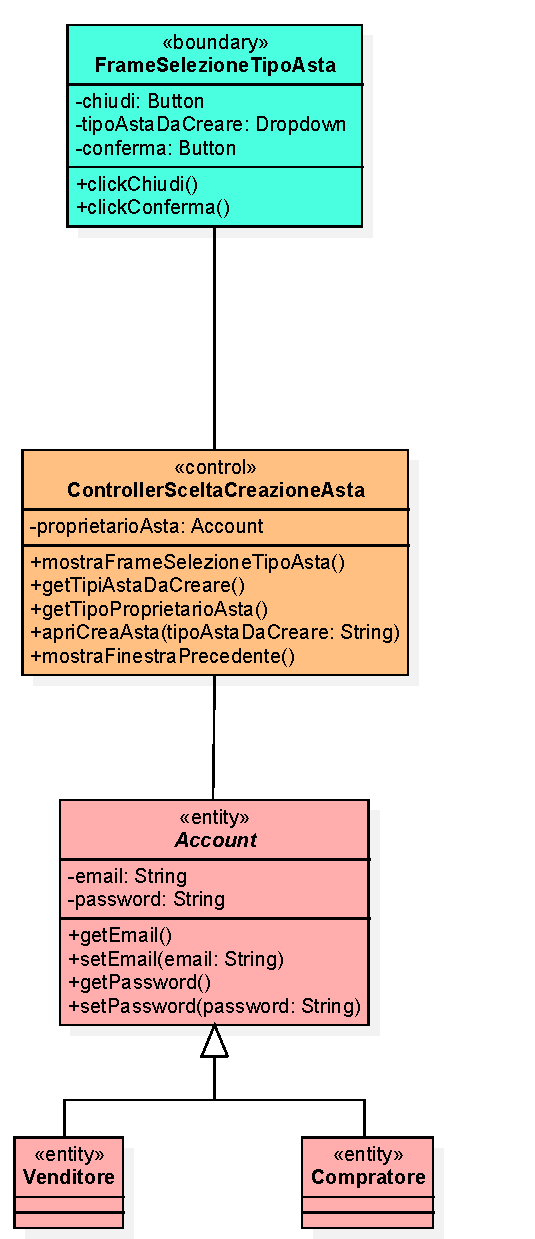
\includegraphics[width=0.5\linewidth]{Immagini/Diagrammi/Class Diagram/Utente che ha effettuato l'accesso/SceltaCreazioneAsta.pdf}
                \caption{Scelta tipo di asta da creare}
            \end{figure}
            
            \begin{figure}[htbp!]
                \centering
                    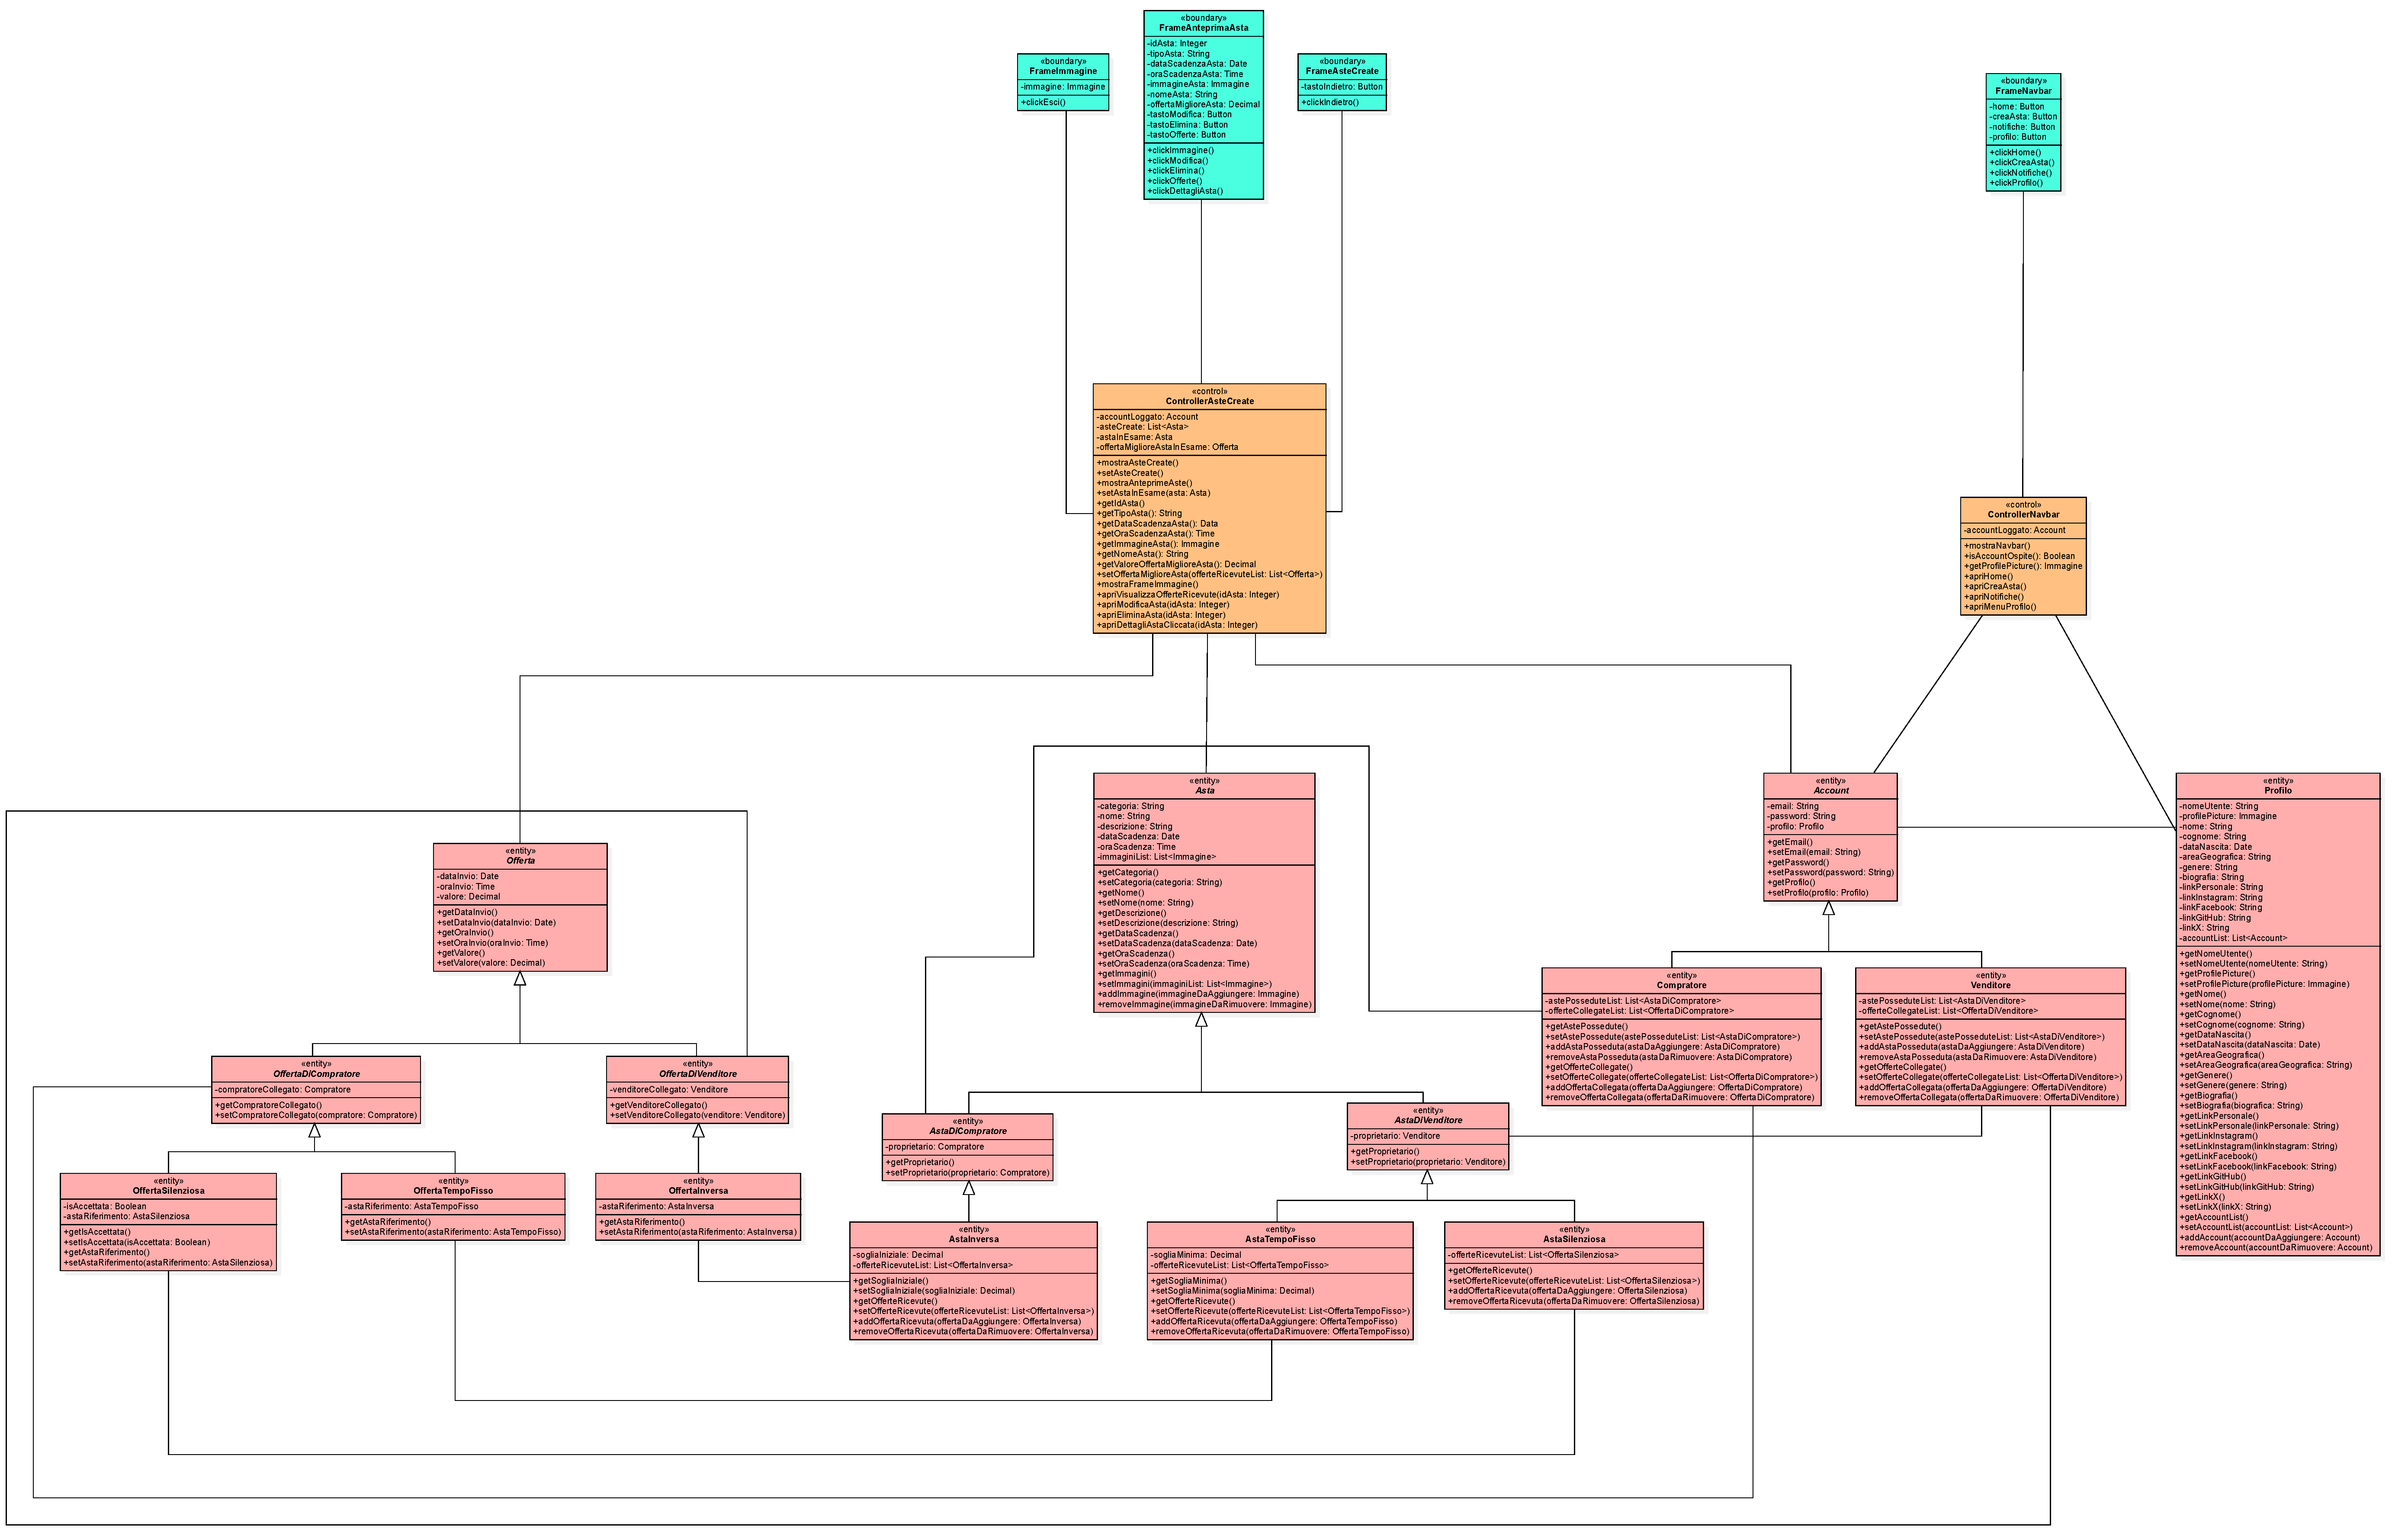
\includegraphics[width=1\linewidth]{Immagini/Diagrammi/Class Diagram/Utente che ha effettuato l'accesso/VisualizzaAsteCreate.pdf}
                \caption{Visualizza aste create}
            \end{figure}

            \begin{figure}[htbp!]
                \centering
                    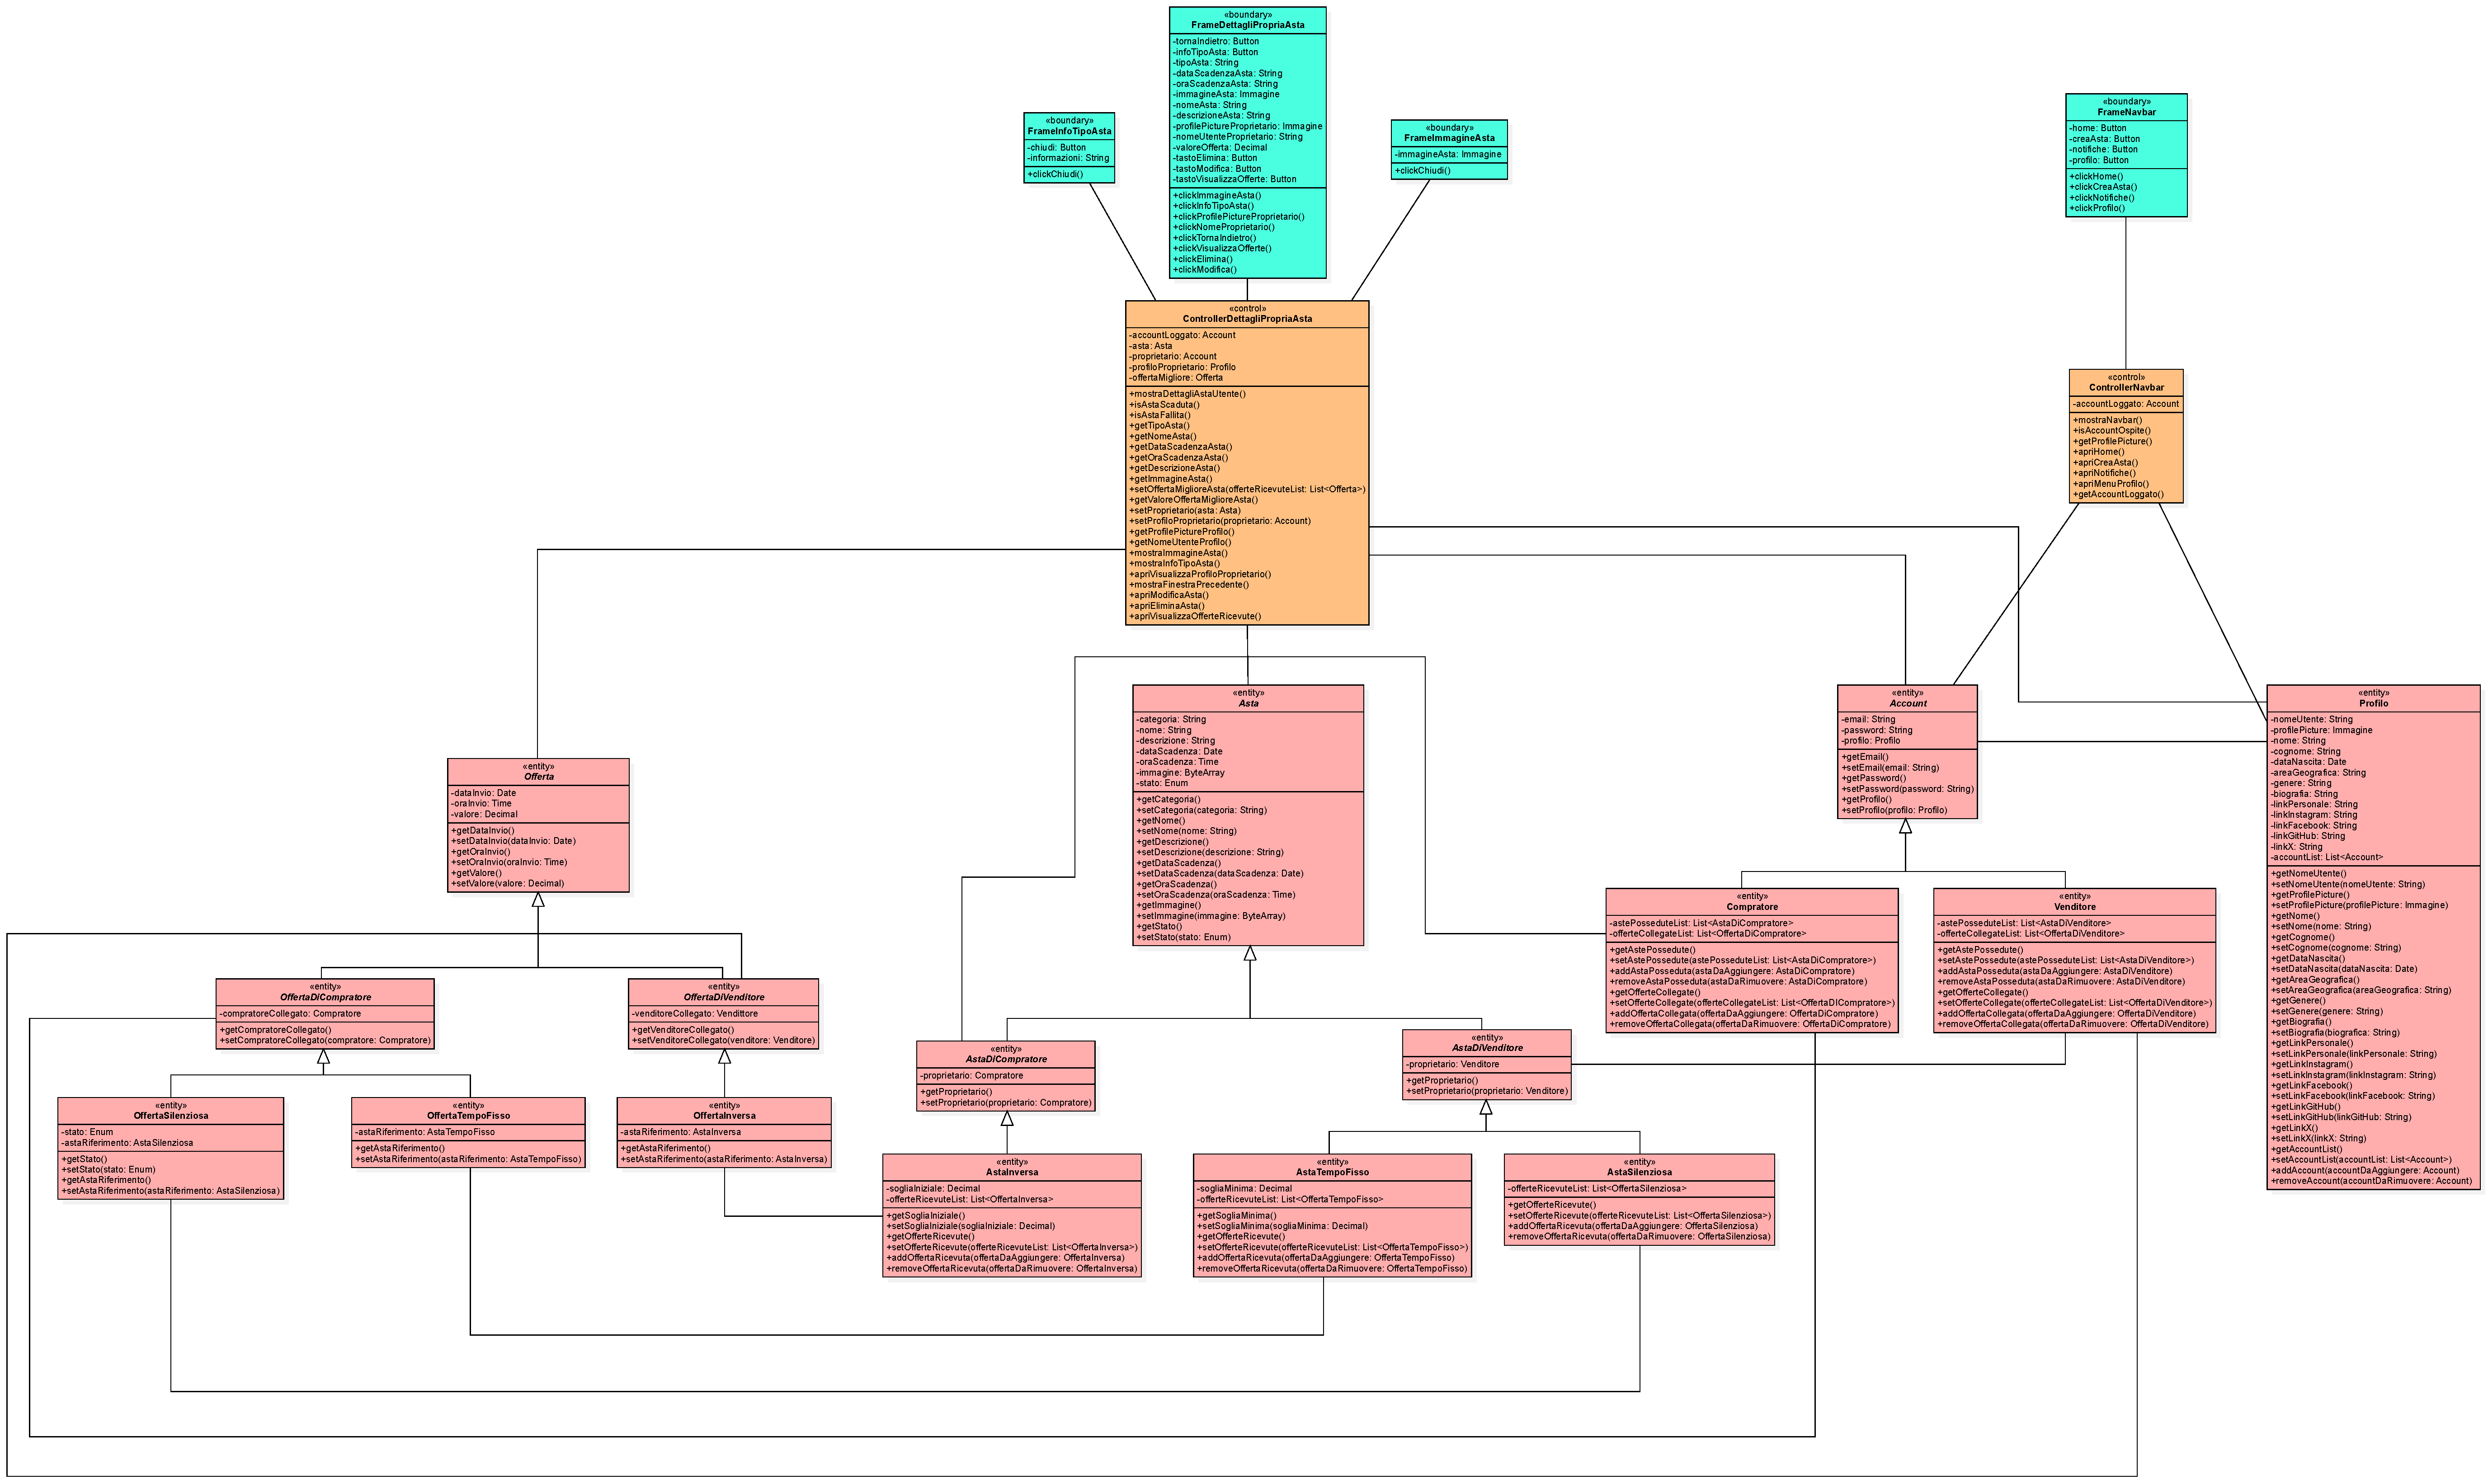
\includegraphics[width=1\linewidth]{Immagini/Diagrammi/Class Diagram/Utente che ha effettuato l'accesso/VisualizzaDettagliPropriaAsta.pdf}
                \caption{Visualizza dettagli della propria asta}
            \end{figure}
            
            \begin{figure}[htbp!]
                \centering
                    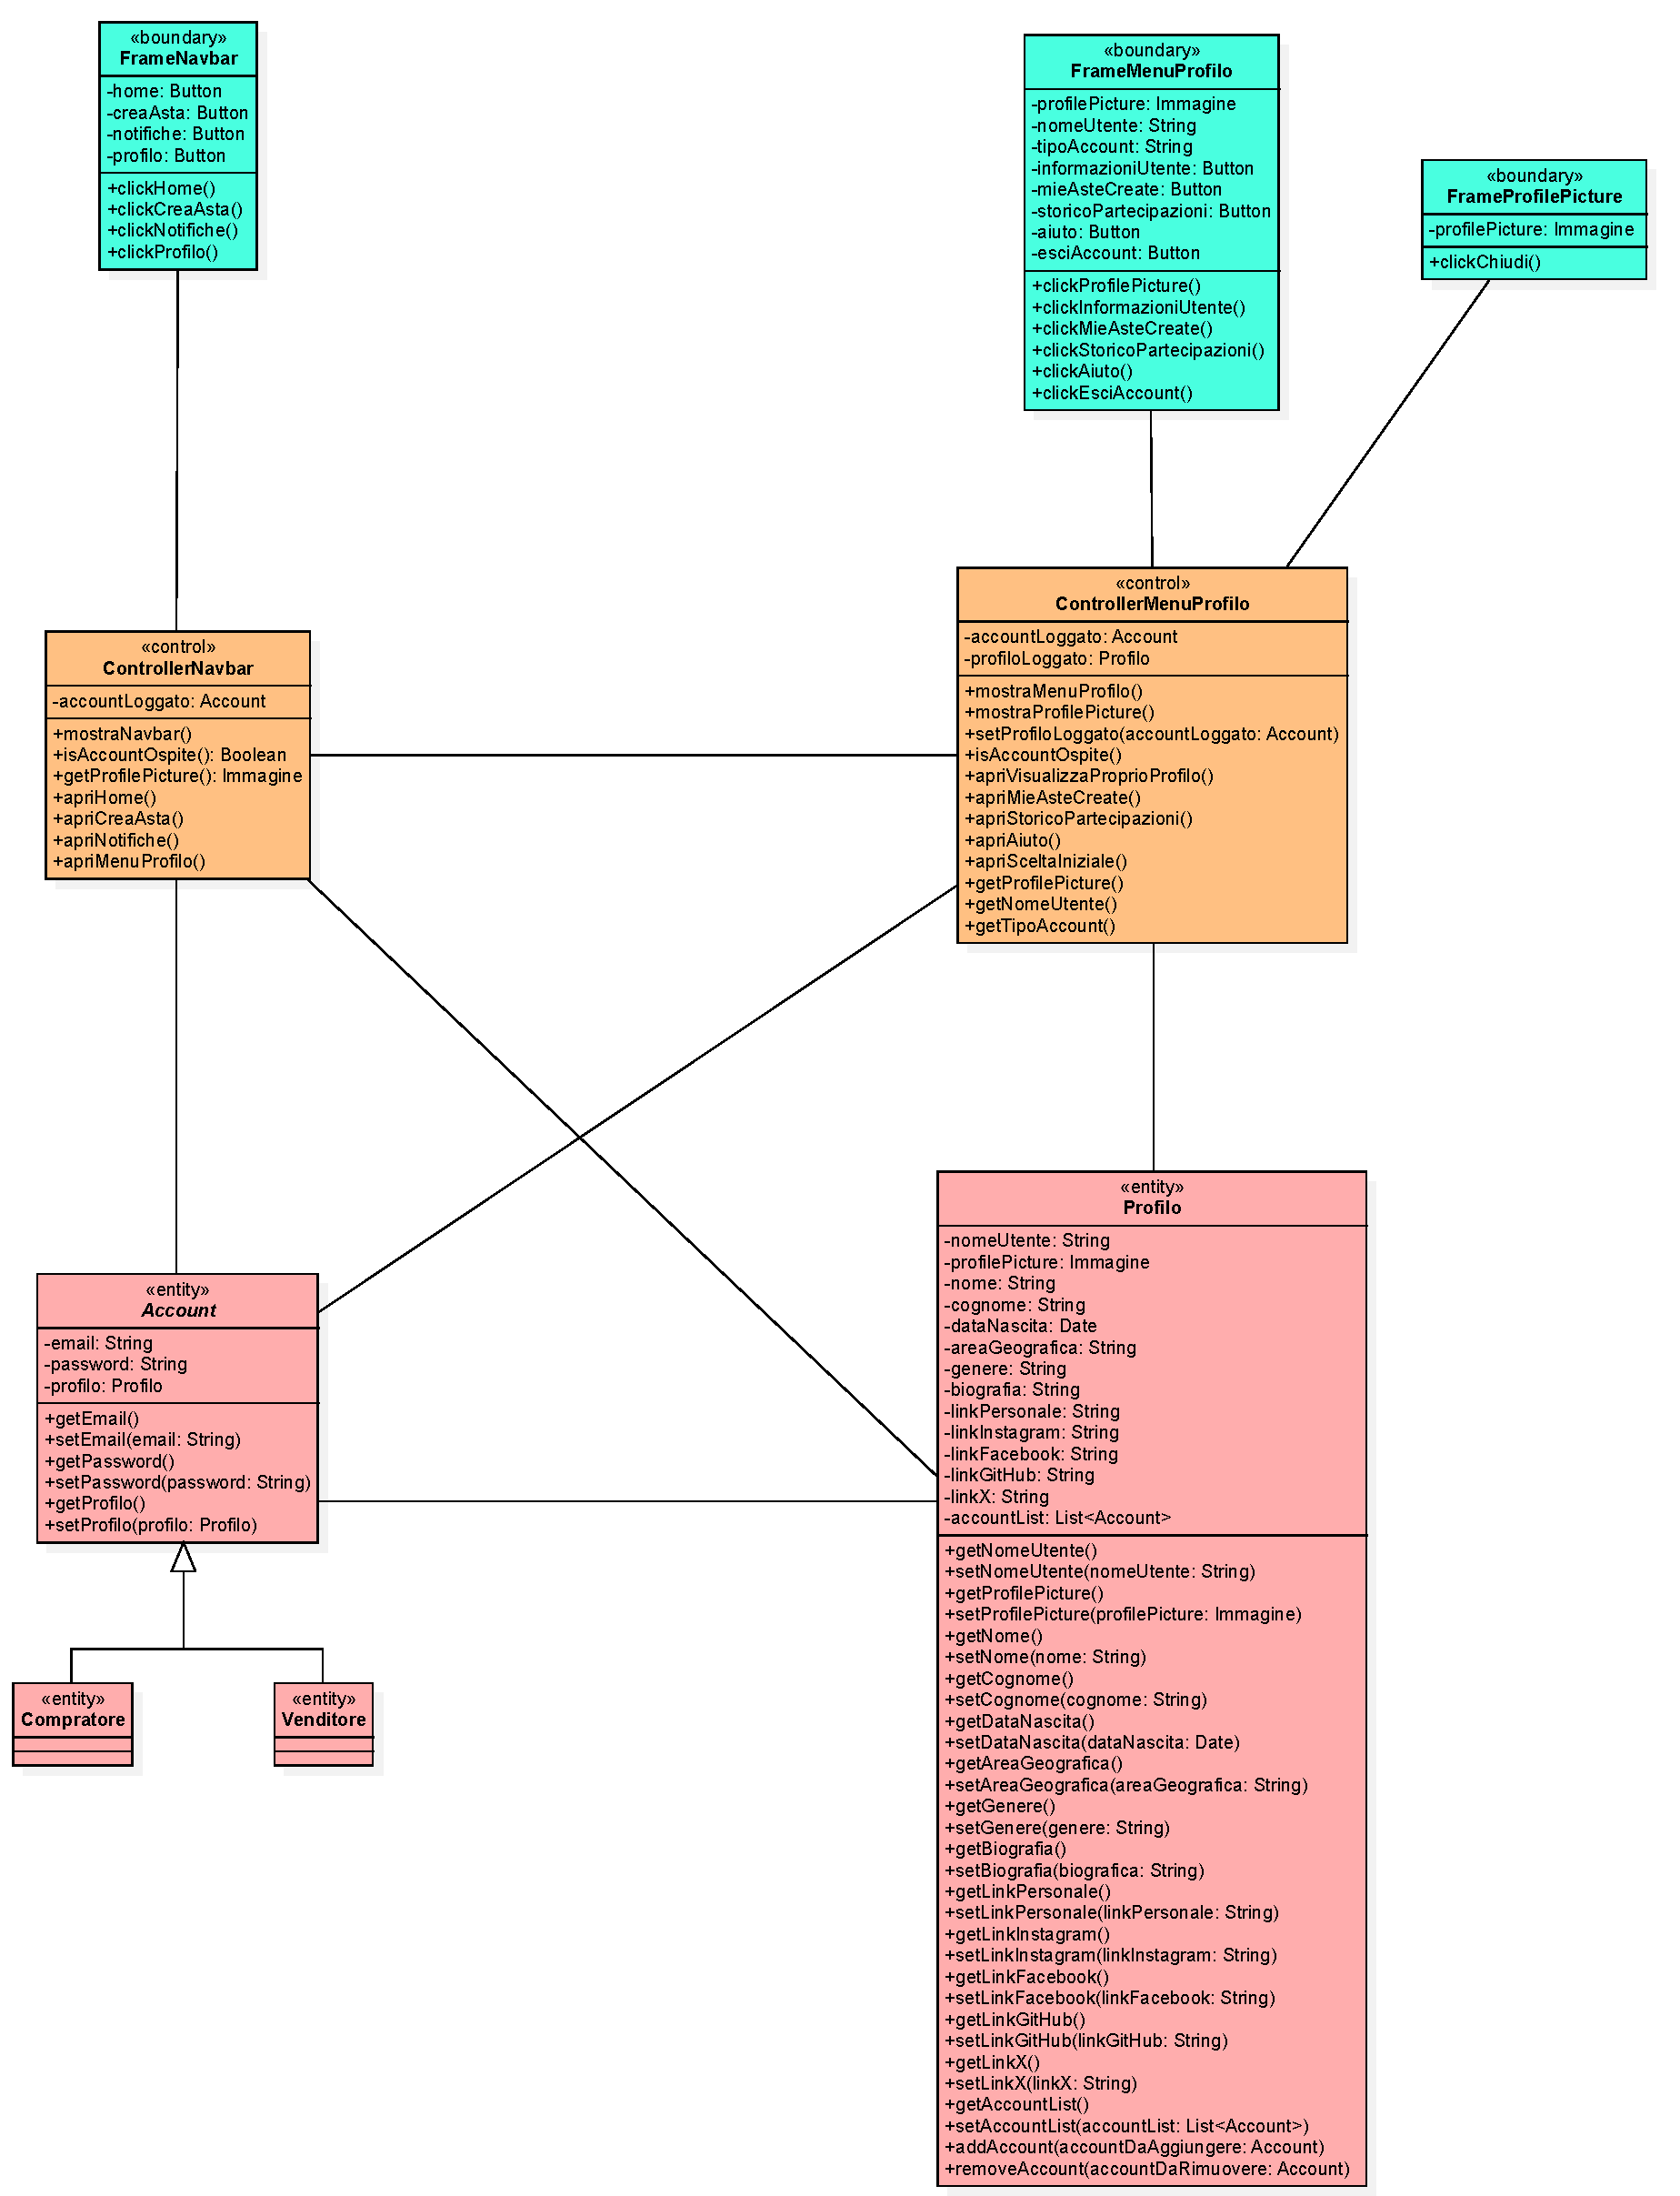
\includegraphics[width=1\linewidth]{Immagini/Diagrammi/Class Diagram/Utente che ha effettuato l'accesso/VisualizzaMenuProfilo.pdf}
                \caption{Visualizza menu profilo}
            \end{figure}
            
            \begin{figure}[htbp!]
                \centering
                    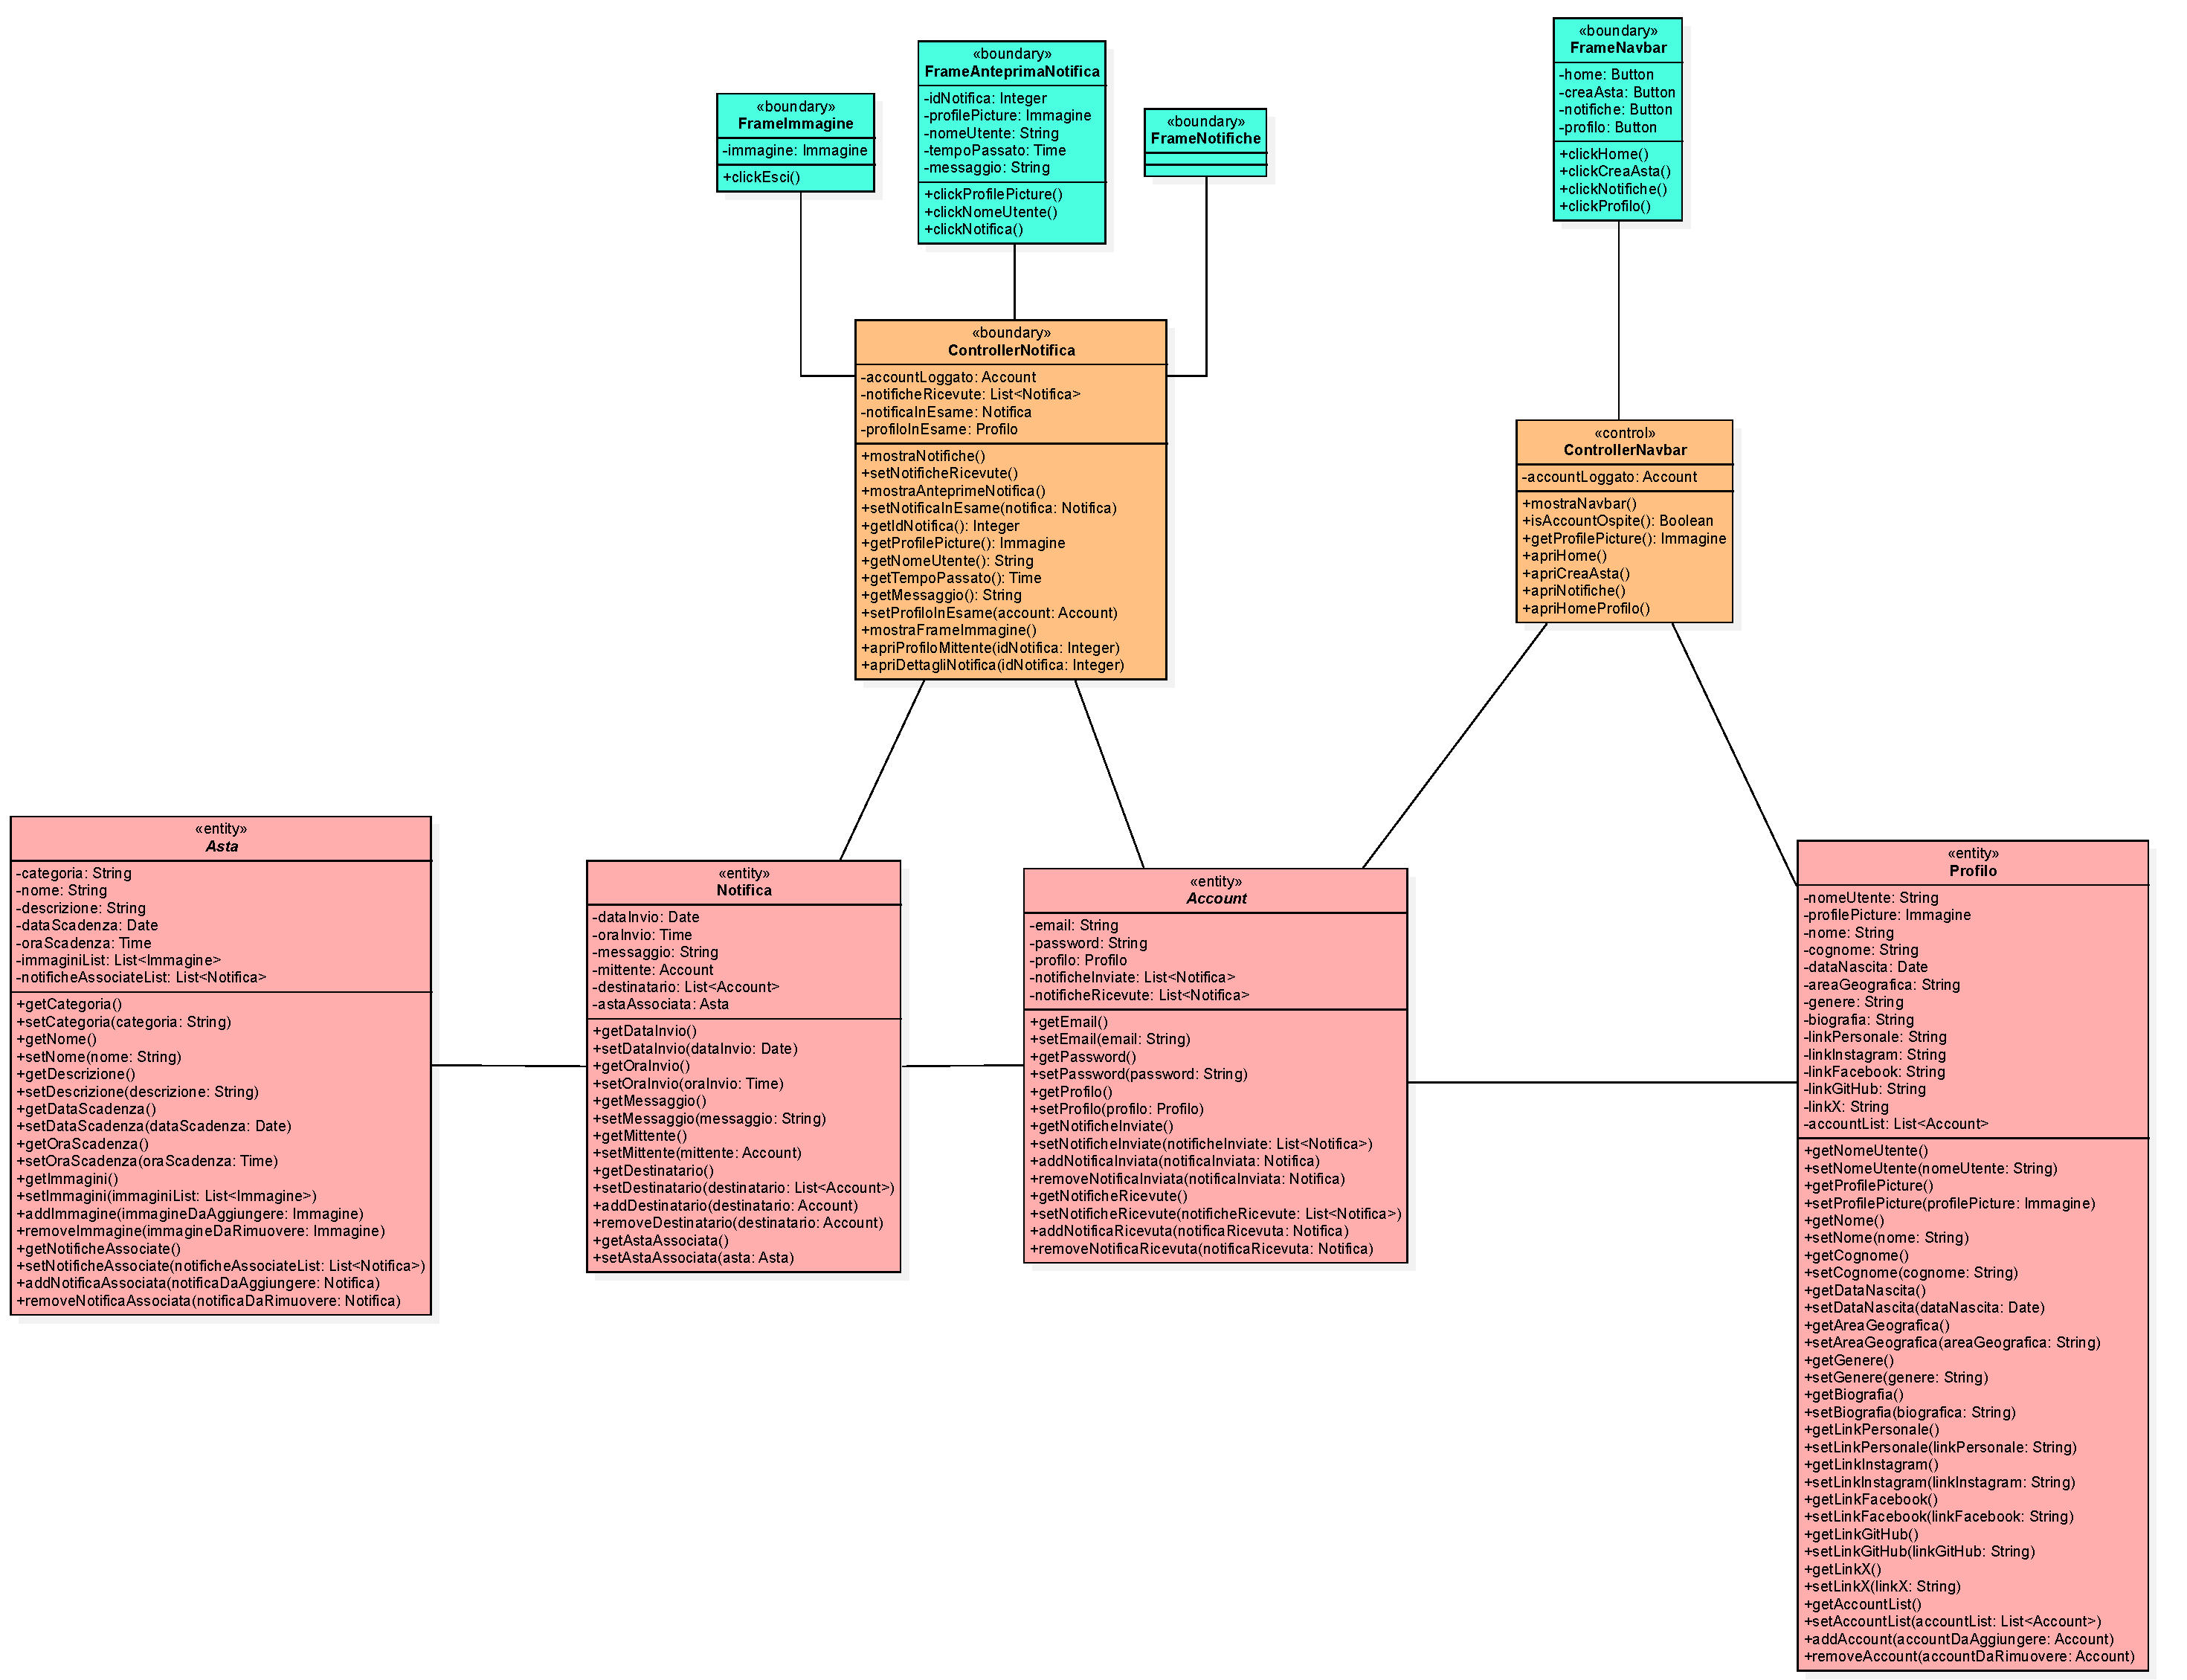
\includegraphics[width=1\linewidth]{Immagini/Diagrammi/Class Diagram/Utente che ha effettuato l'accesso/VisualizzaNotifiche.pdf}
                \caption{Visualizza notifiche}
            \end{figure}
            
            \begin{figure}[htbp!]
                \centering
                    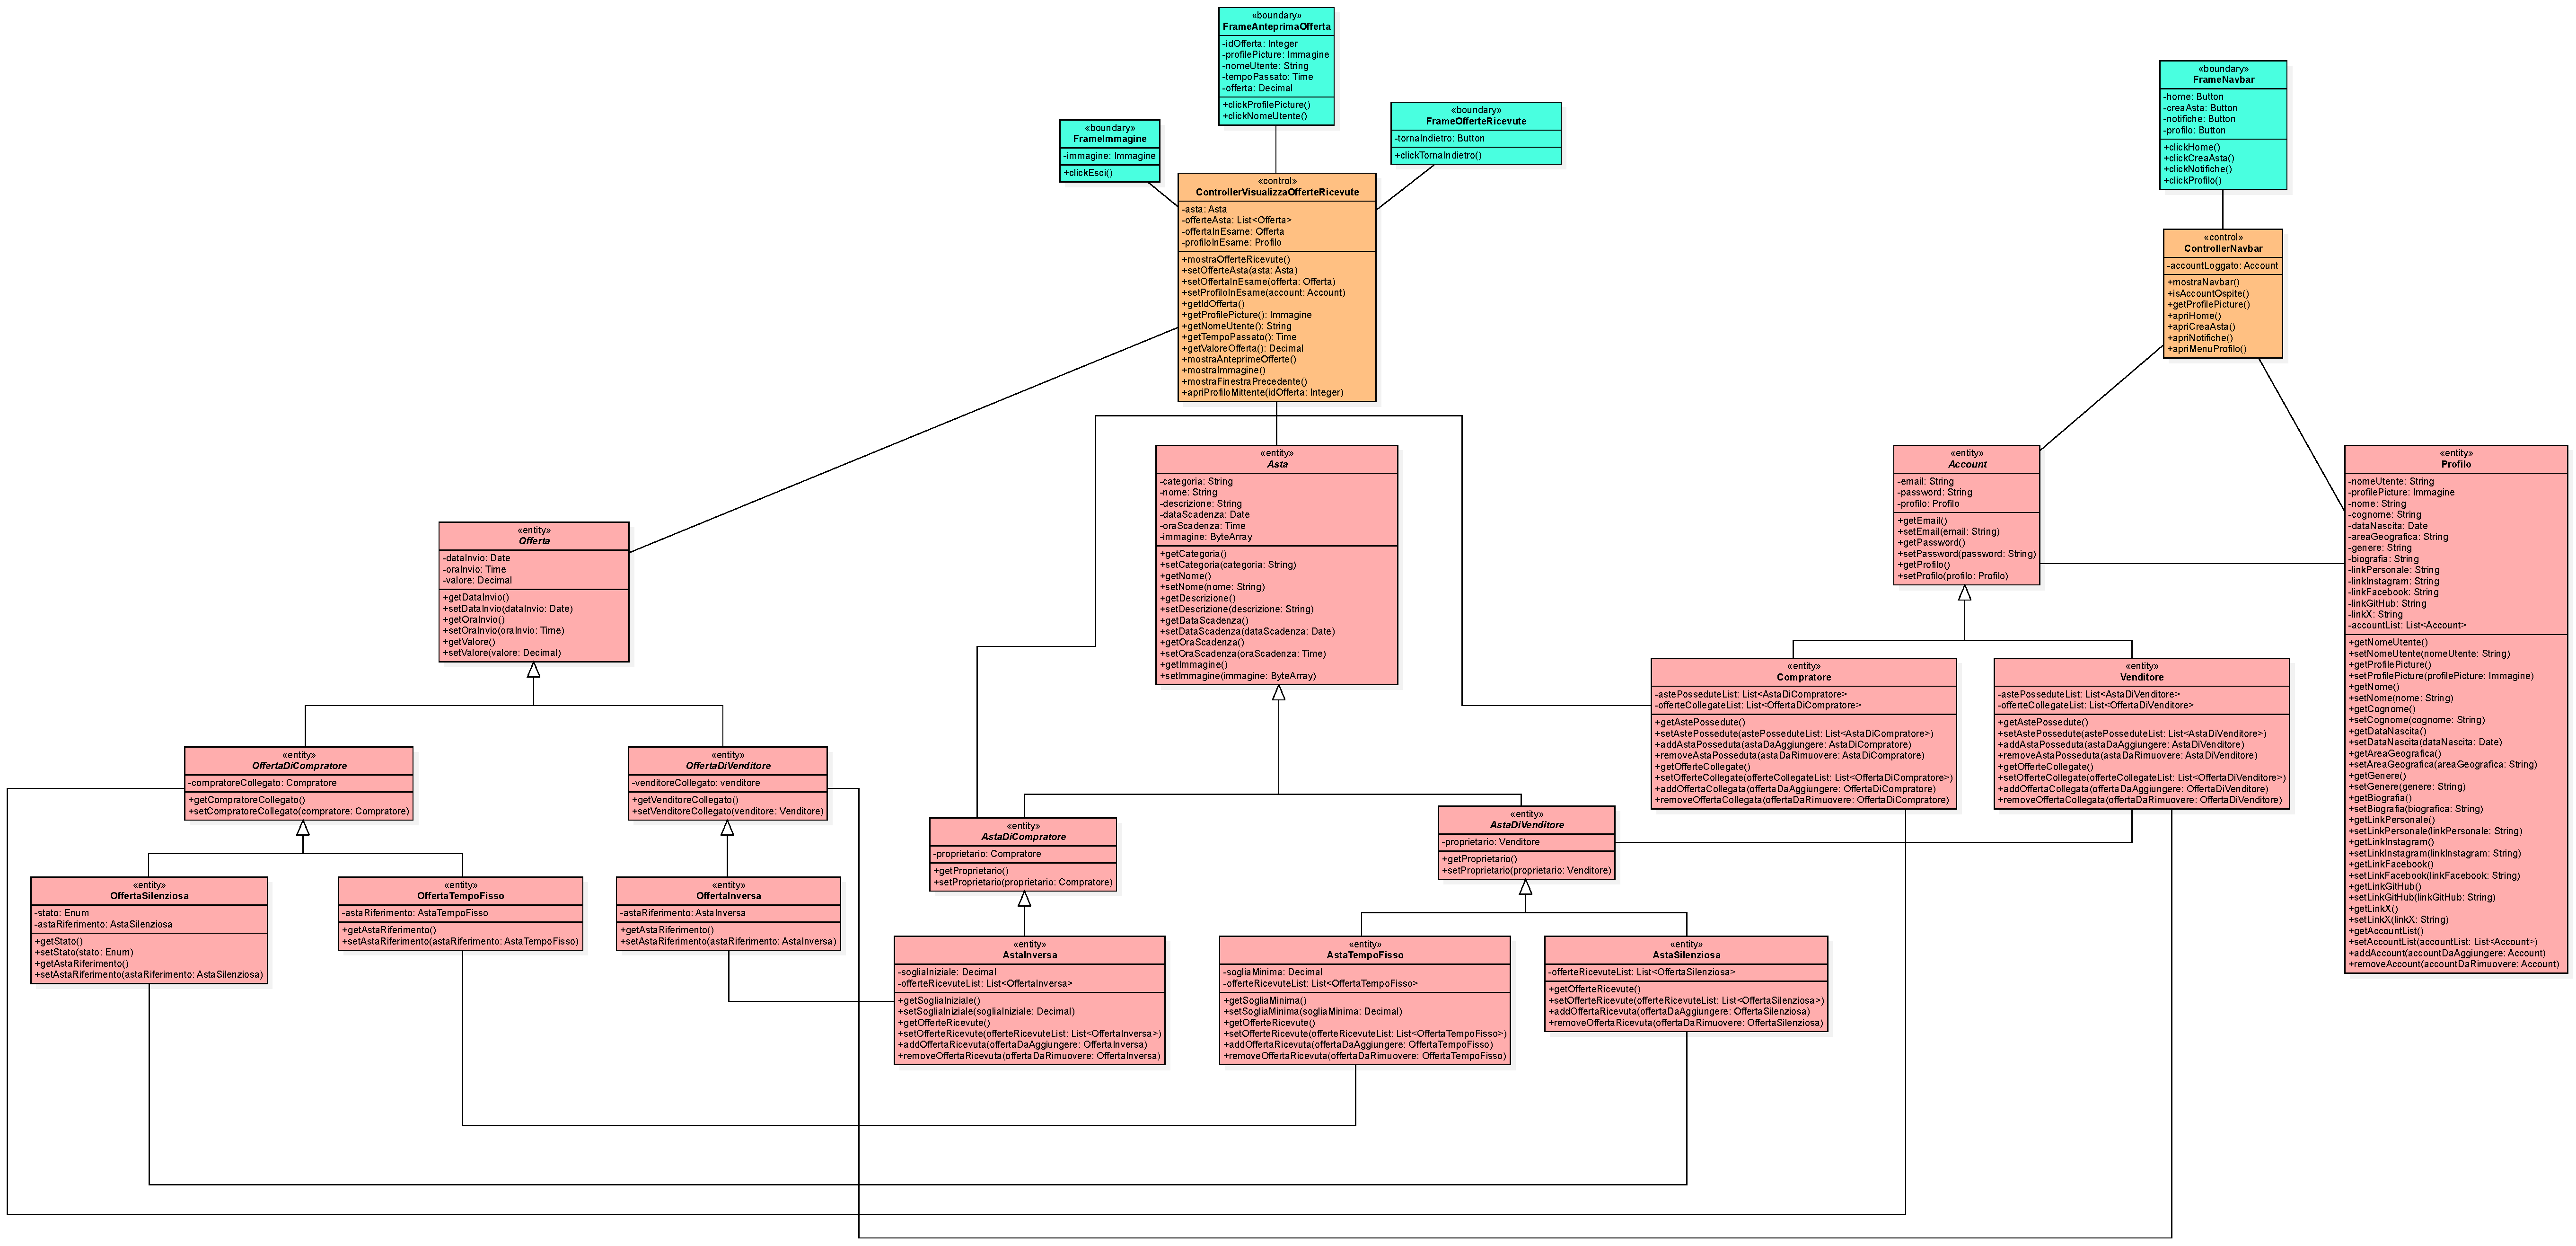
\includegraphics[width=1\linewidth]{Immagini/Diagrammi/Class Diagram/Utente che ha effettuato l'accesso/VisualizzaOfferteRicevute.pdf}
                \caption{Visualizza offerte ricevute}
            \end{figure}
            
            \begin{figure}[htbp!]
                \centering
                    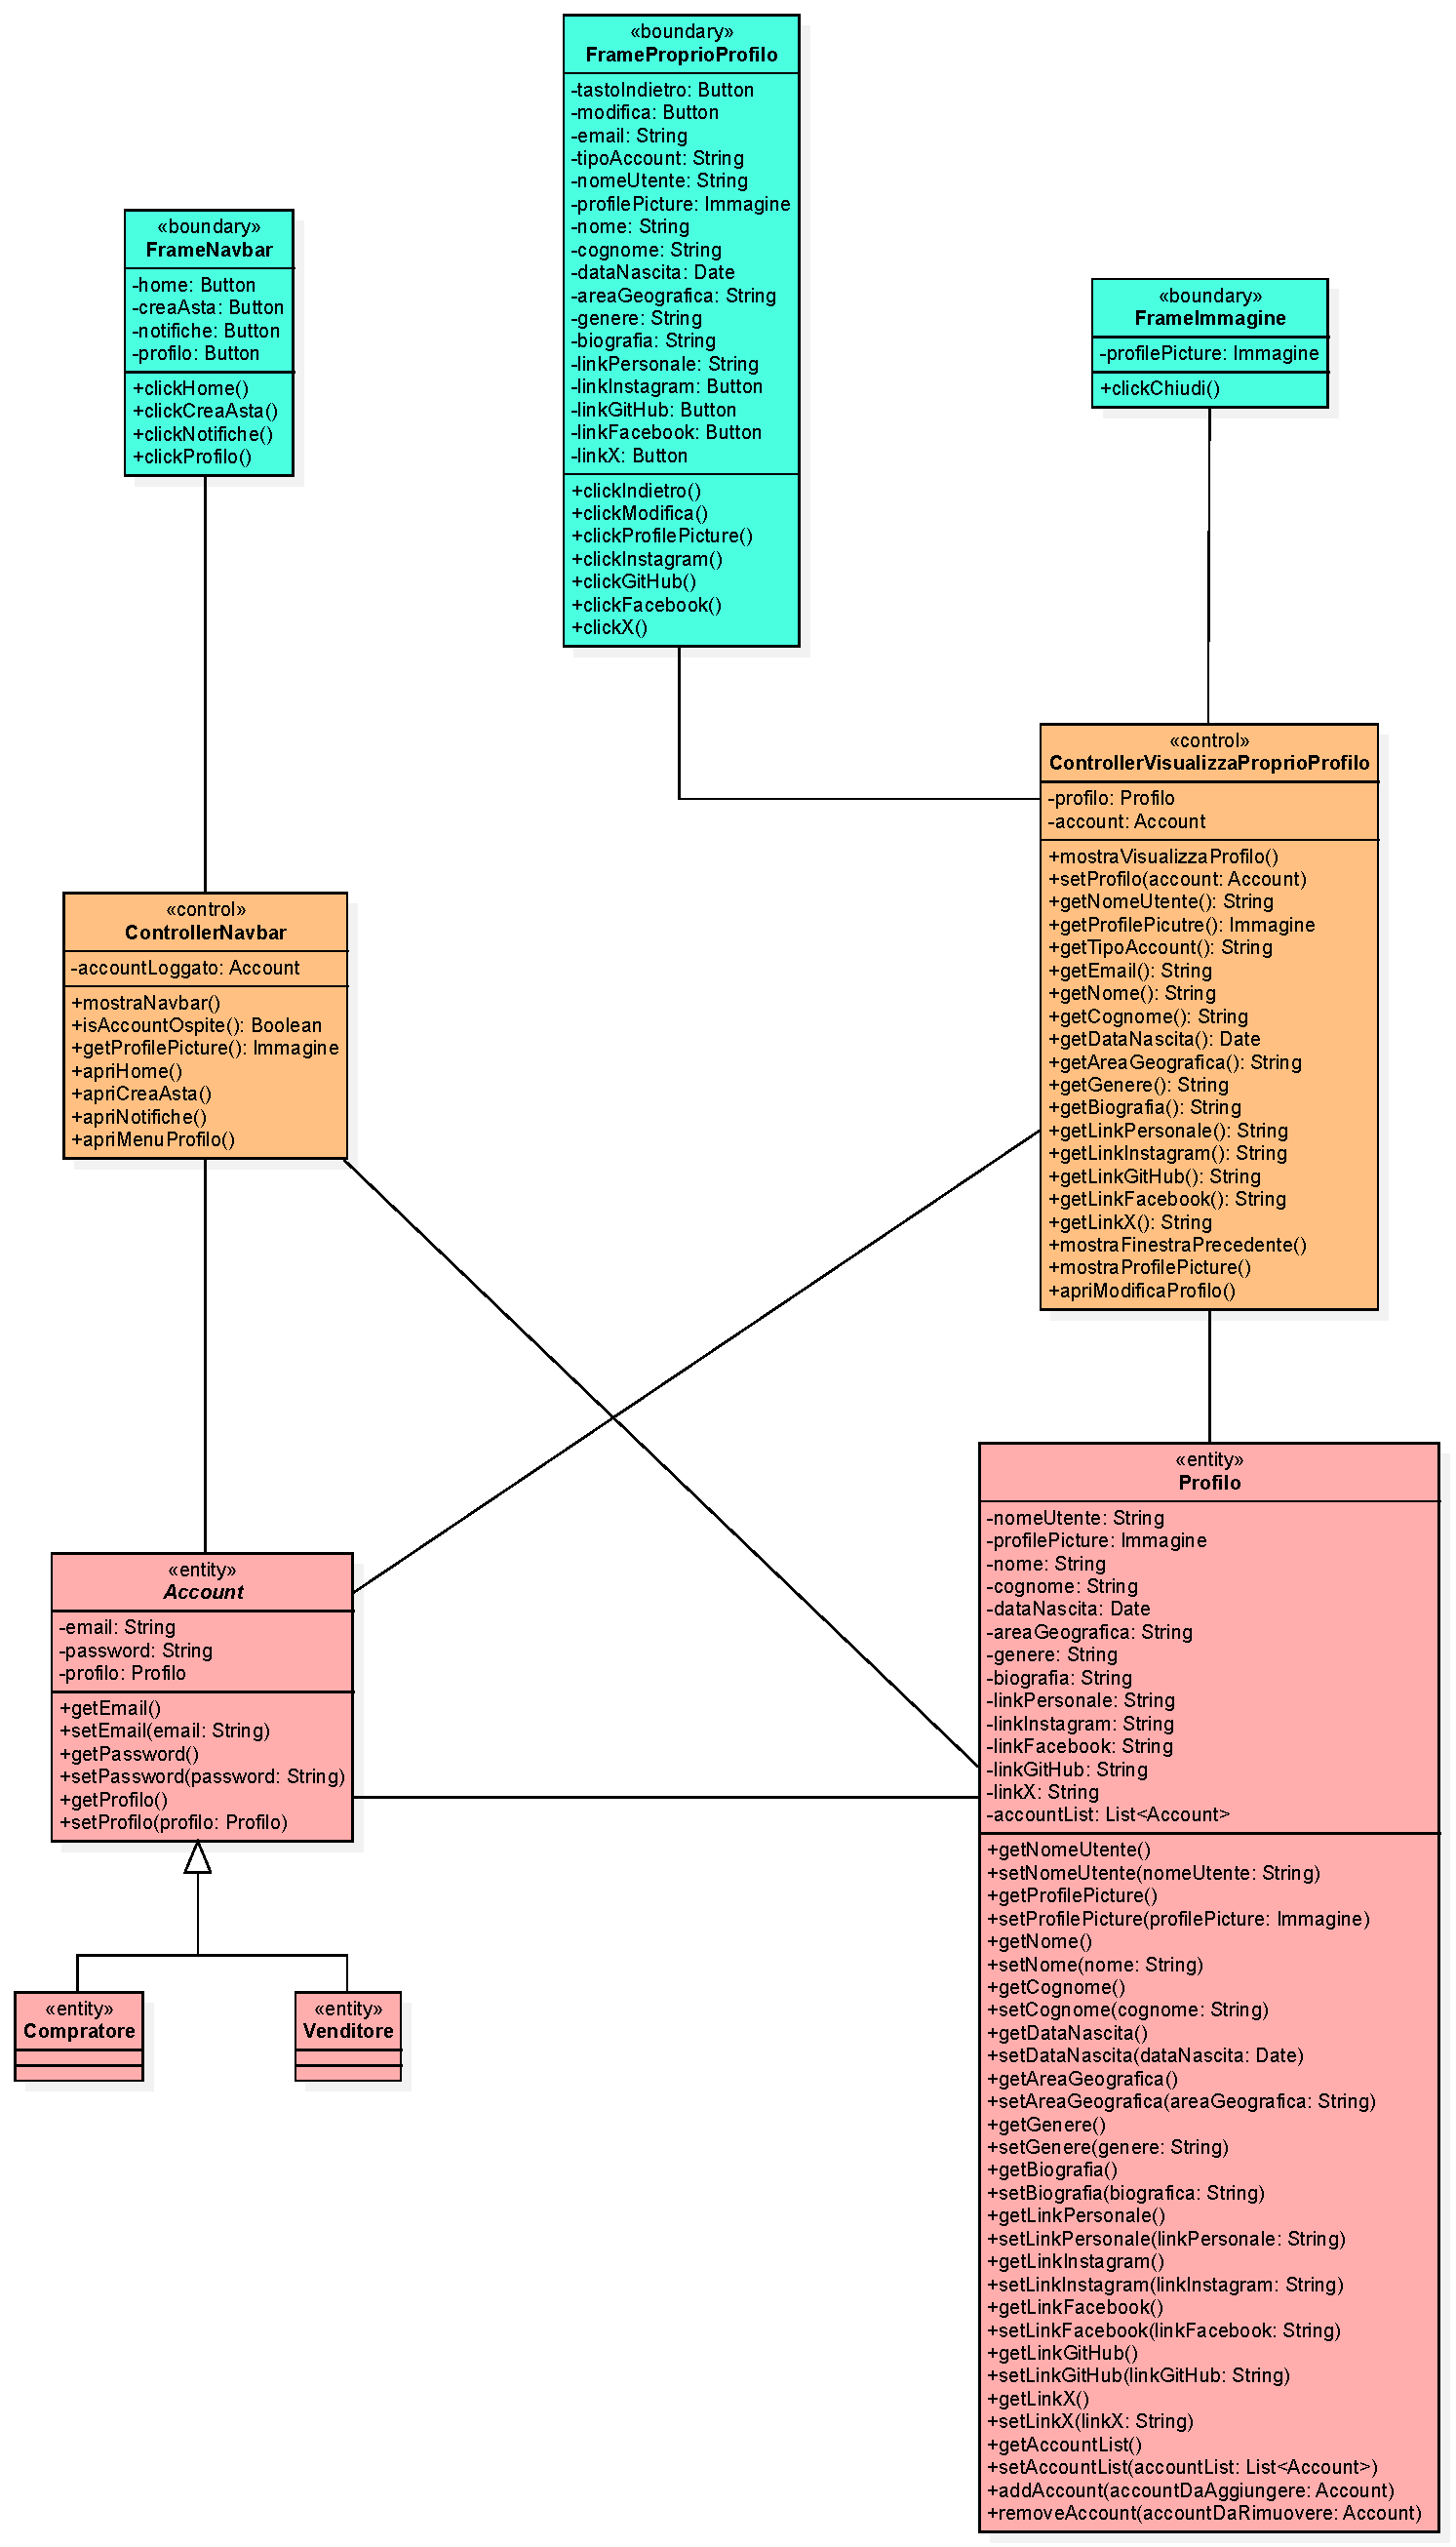
\includegraphics[width=0.75\linewidth]{Immagini/Diagrammi/Class Diagram/Utente che ha effettuato l'accesso/VisualizzaProprioProfilo.pdf}
                \caption{Visualizza profilo personale}
            \end{figure}
            
            \begin{figure}[htbp!]
                \centering
                    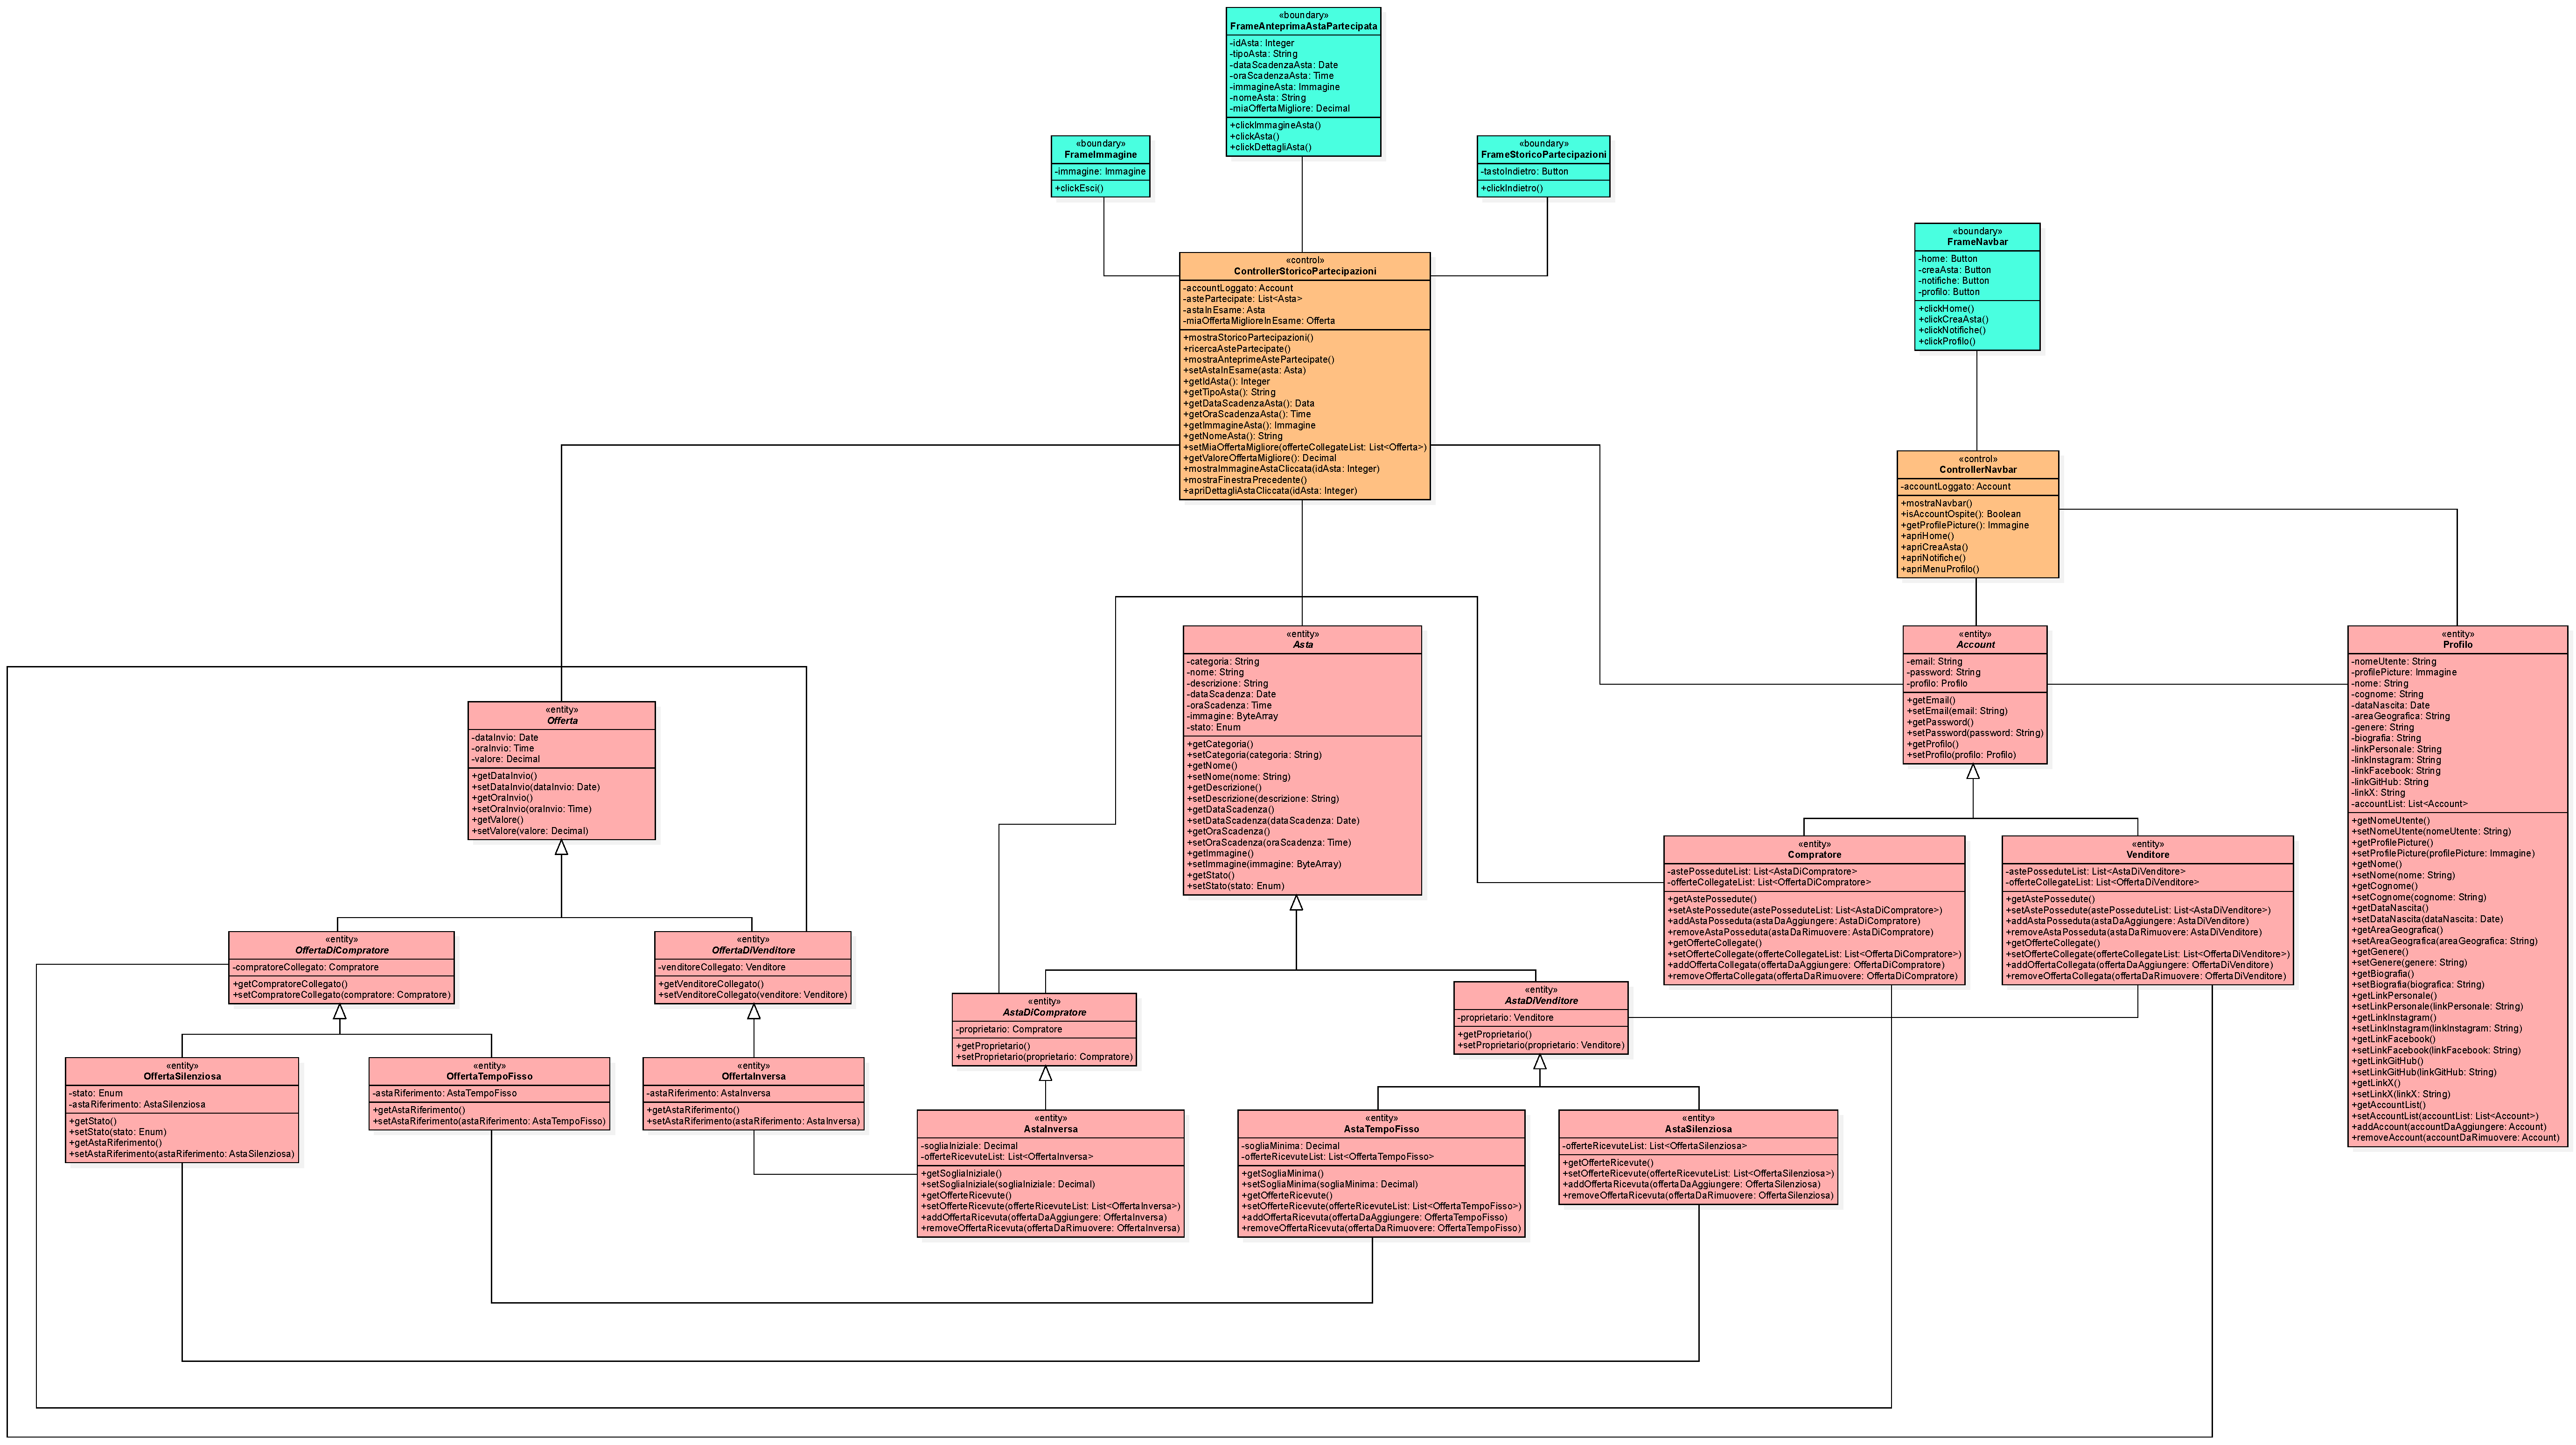
\includegraphics[width=1\linewidth]{Immagini/Diagrammi/Class Diagram/Utente che ha effettuato l'accesso/VisualizzaStoricoPartecipazioni.pdf}
                \caption{Visualizza aste partecipate}
            \end{figure}
            
            \begin{figure}[htbp!]
                \centering
                    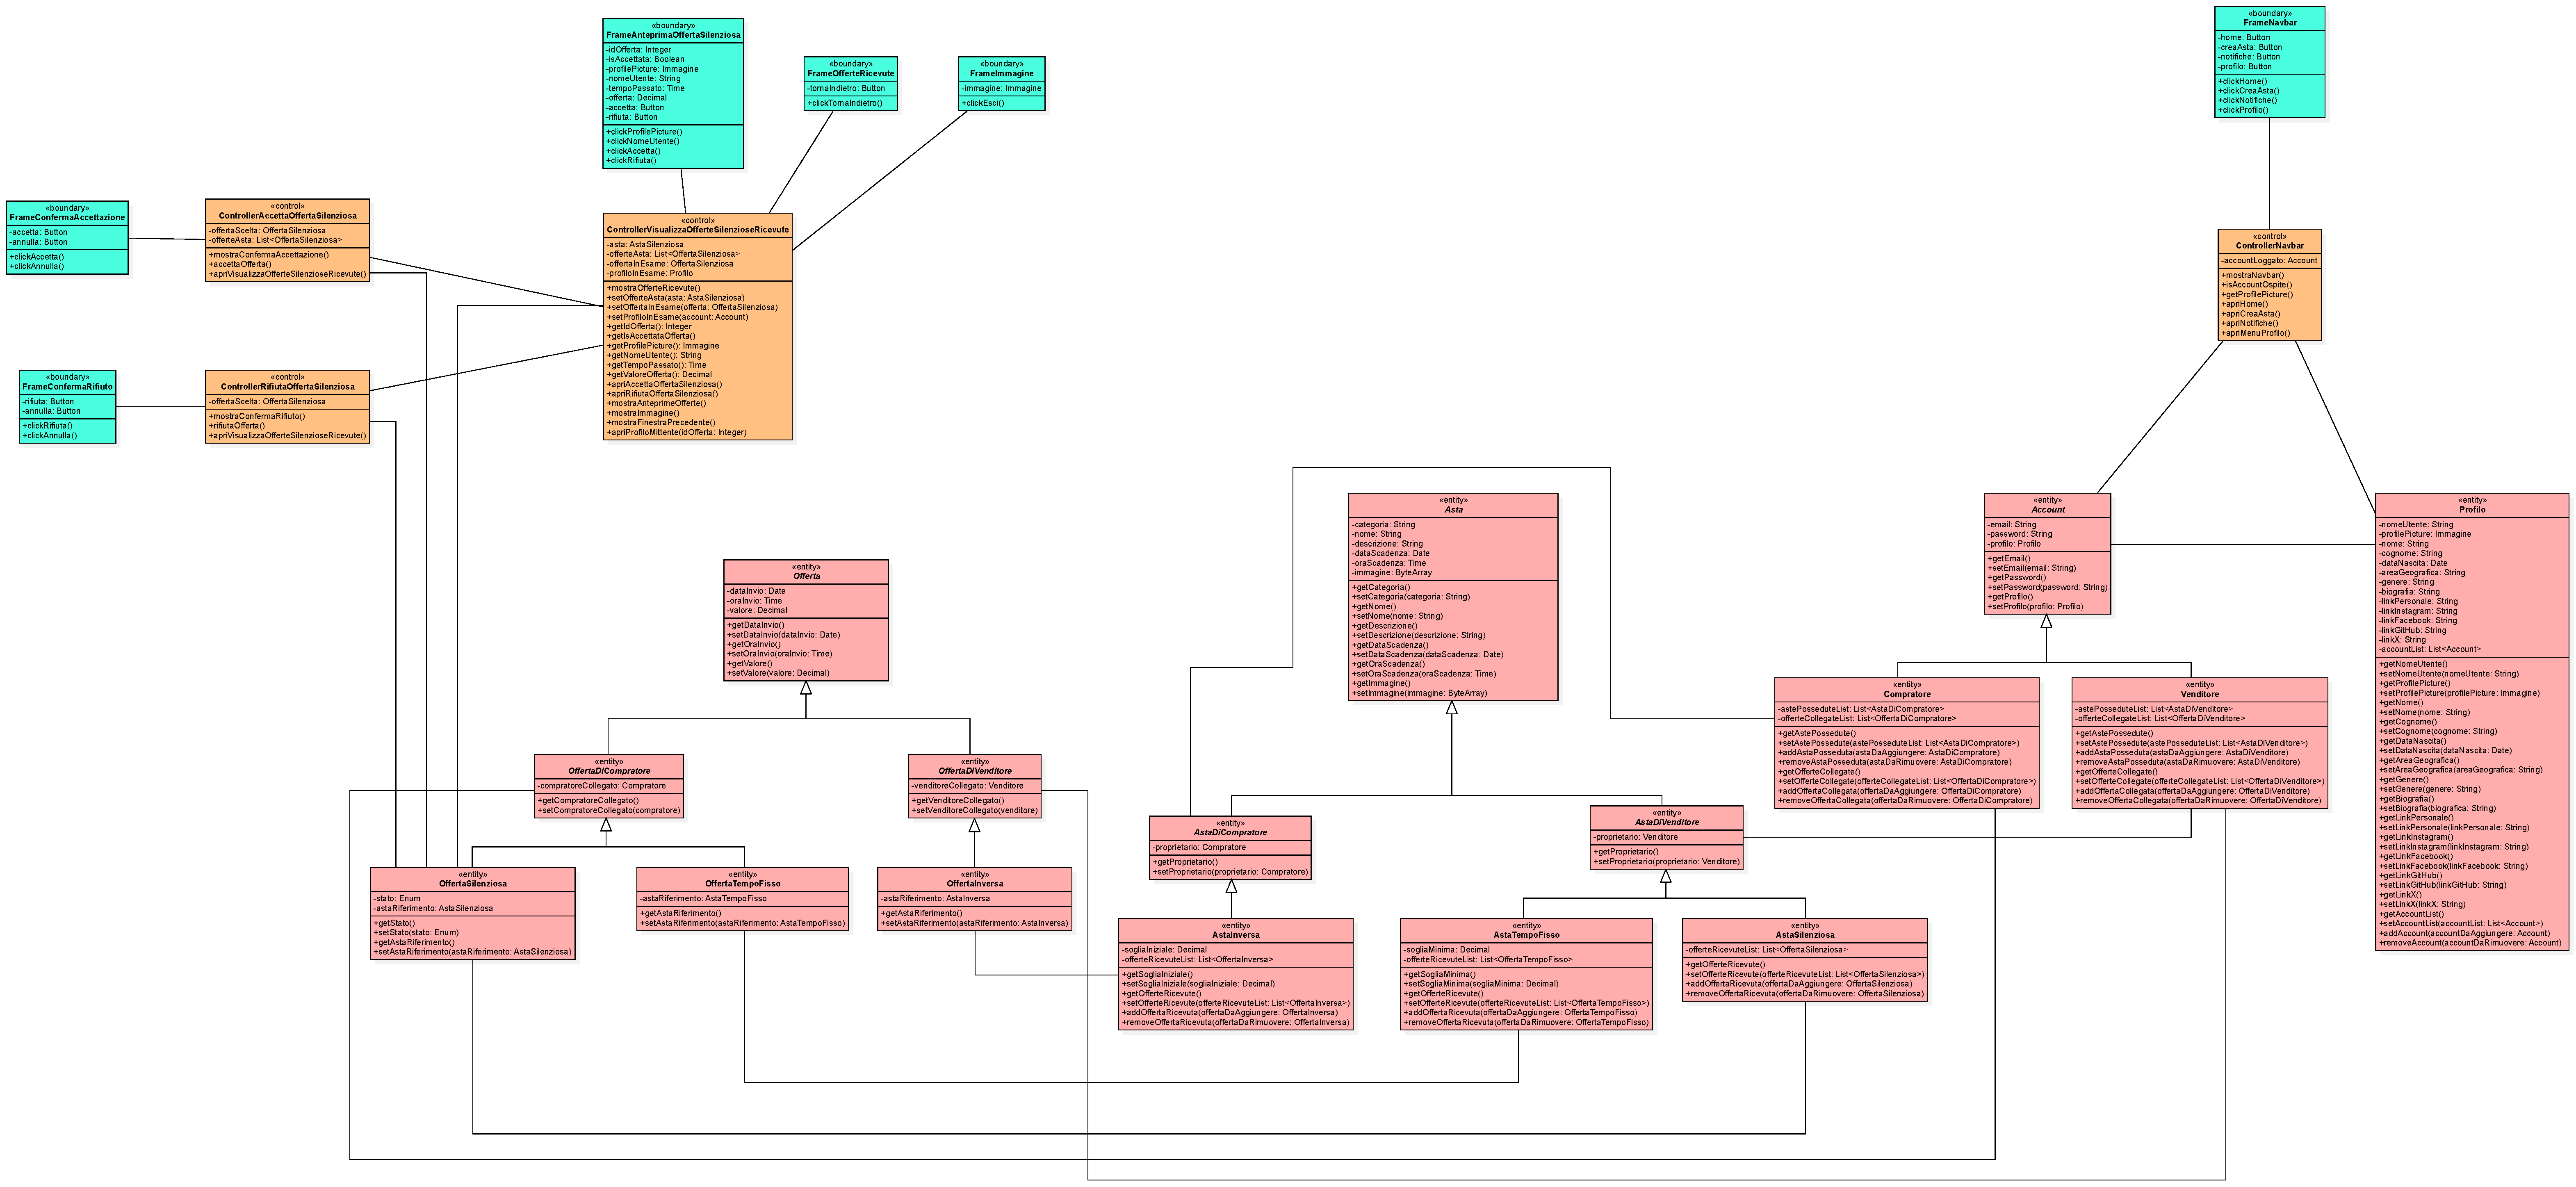
\includegraphics[width=1\linewidth]{Immagini/Diagrammi/Class Diagram/Venditore e compratore/AccettaRifiutaOffertaSilenziosa.pdf}
                \caption{Accetta o rifiuta un'offerta per un'asta silenziosa}
            \end{figure}
            
            \begin{figure}[htbp!]
                \centering
                    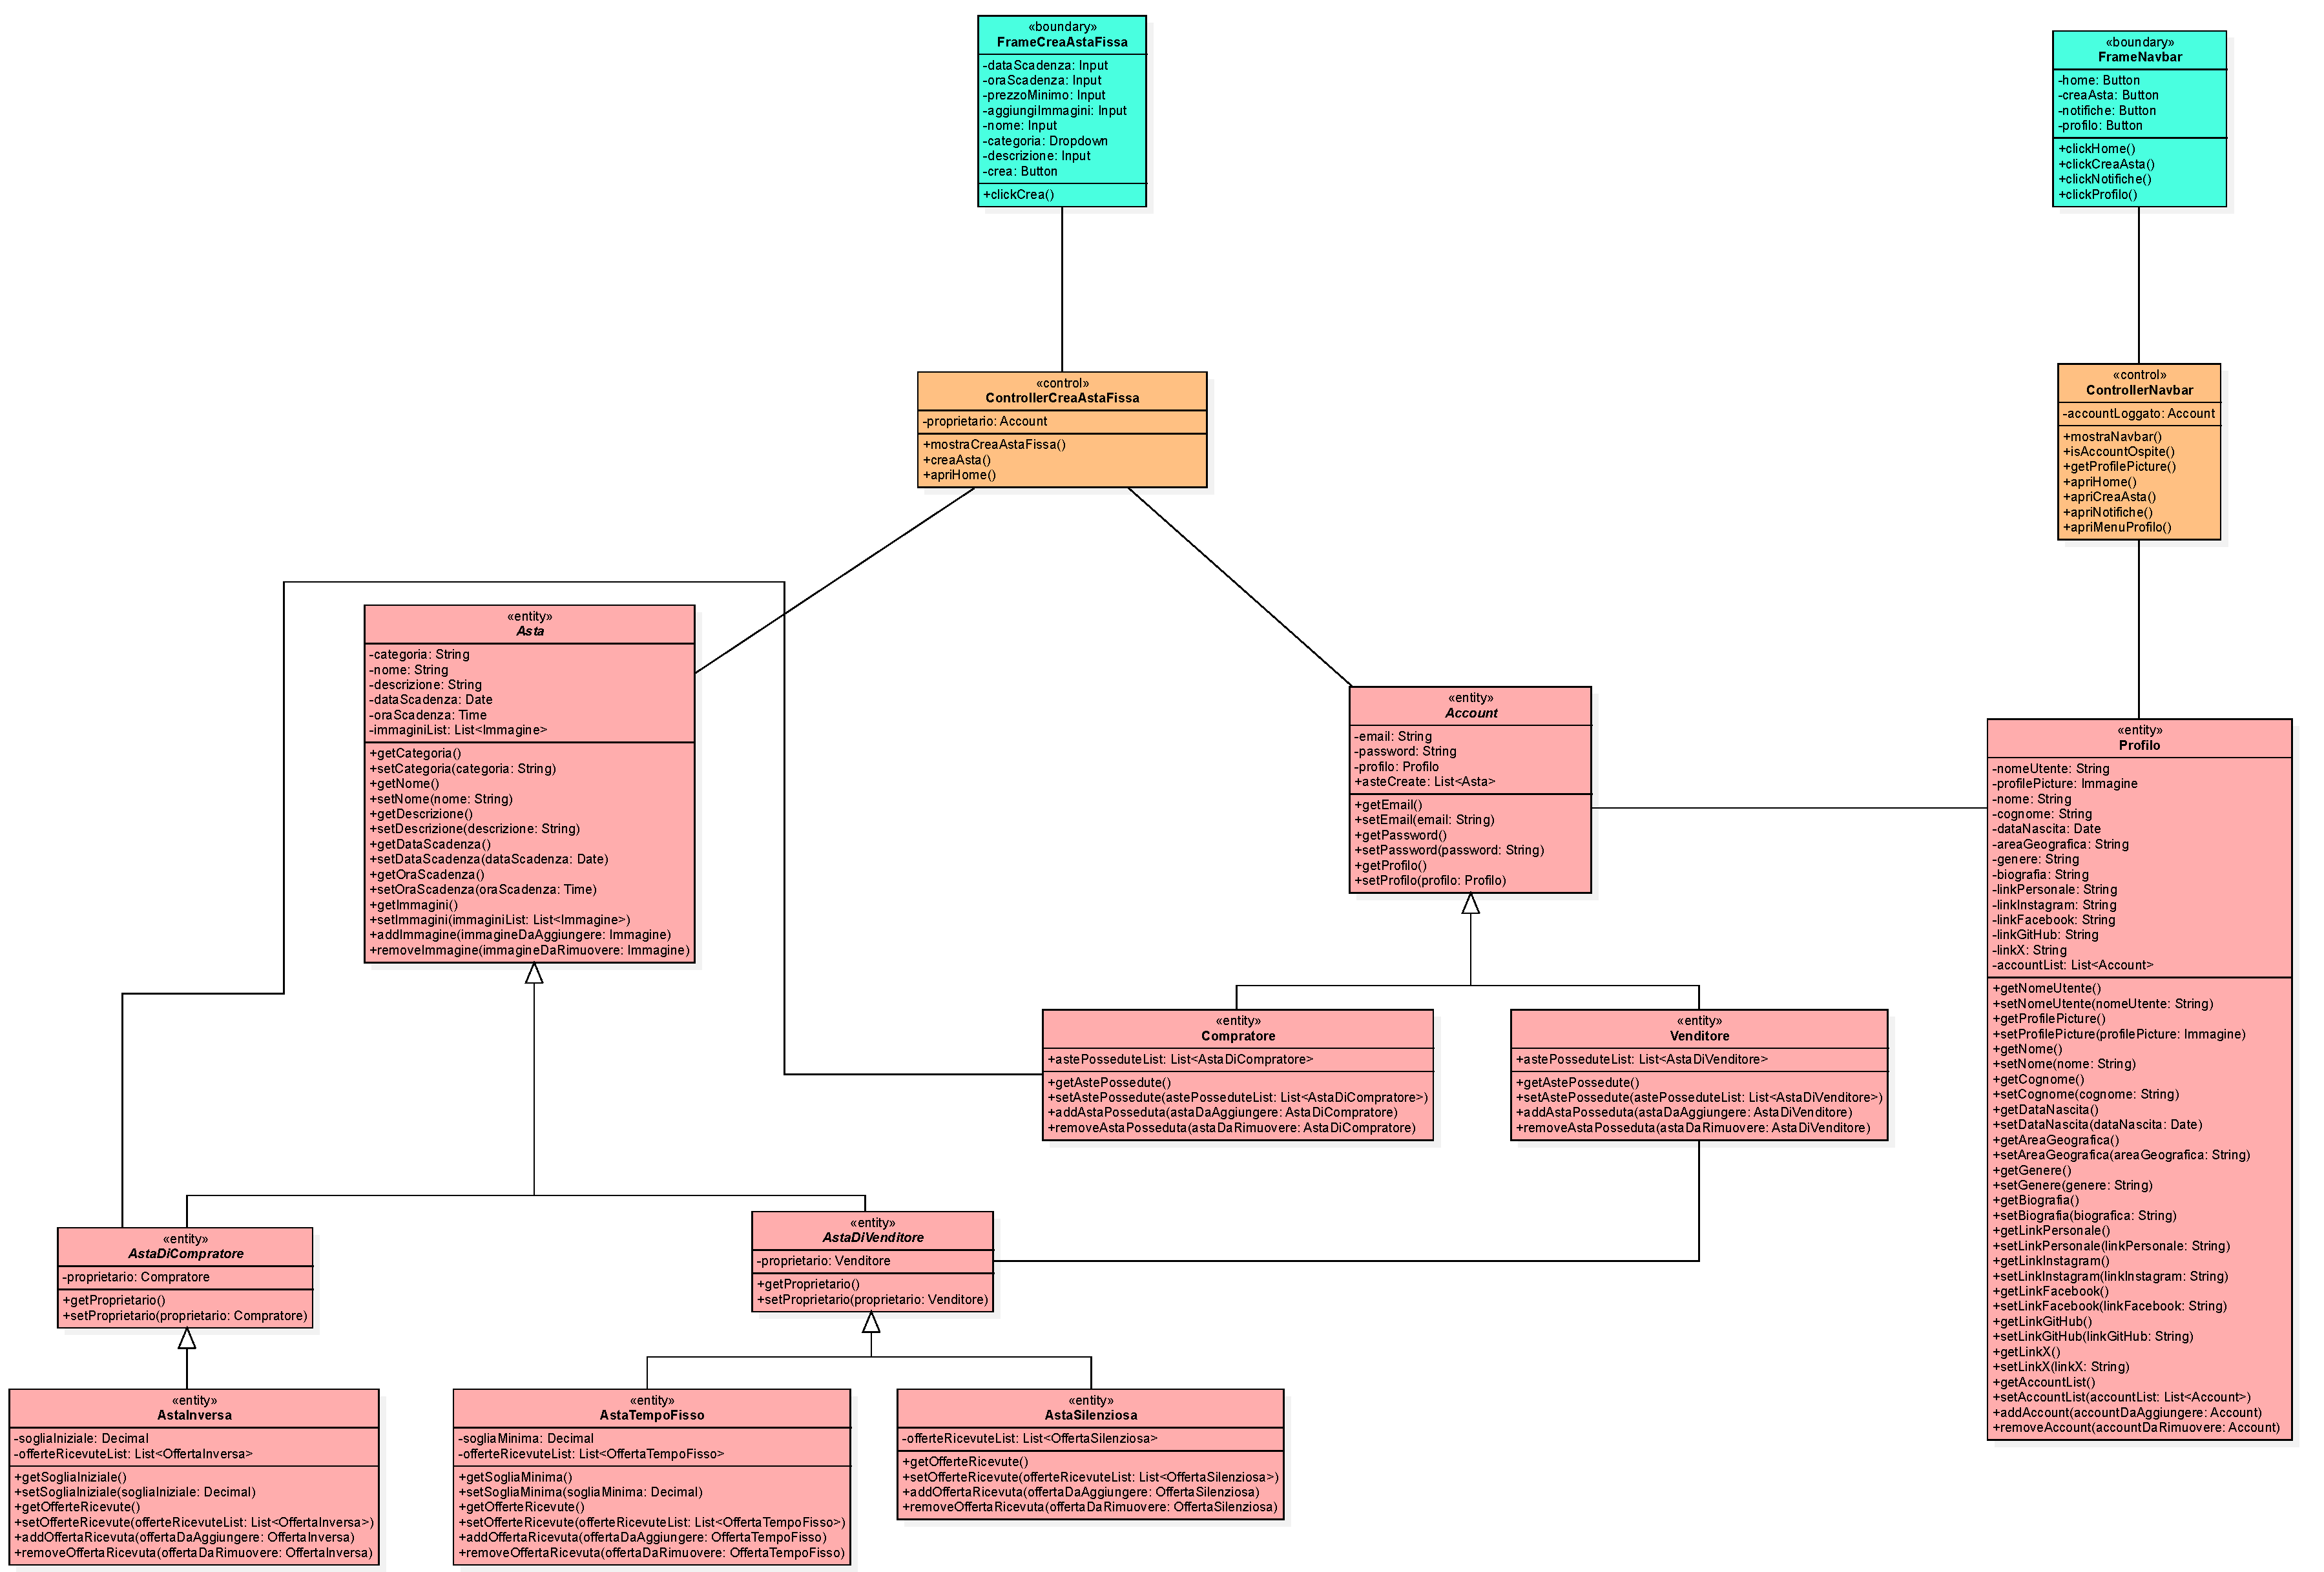
\includegraphics[width=1\linewidth]{Immagini/Diagrammi/Class Diagram/Venditore e compratore/CreaAstaFissa.pdf}
                \caption{Crea un'asta a tempo fisso}
            \end{figure}
            
            \begin{figure}[htbp!]
                \centering
                    \includegraphics[width=1\linewidth]{Immagini/Diagrammi/Class Diagram/Venditore e compratore/CreaAstaInversa.pdf}
                \caption{Crea un'asta inversa}
            \end{figure}
            
            \begin{figure}[htbp!]
                \centering
                    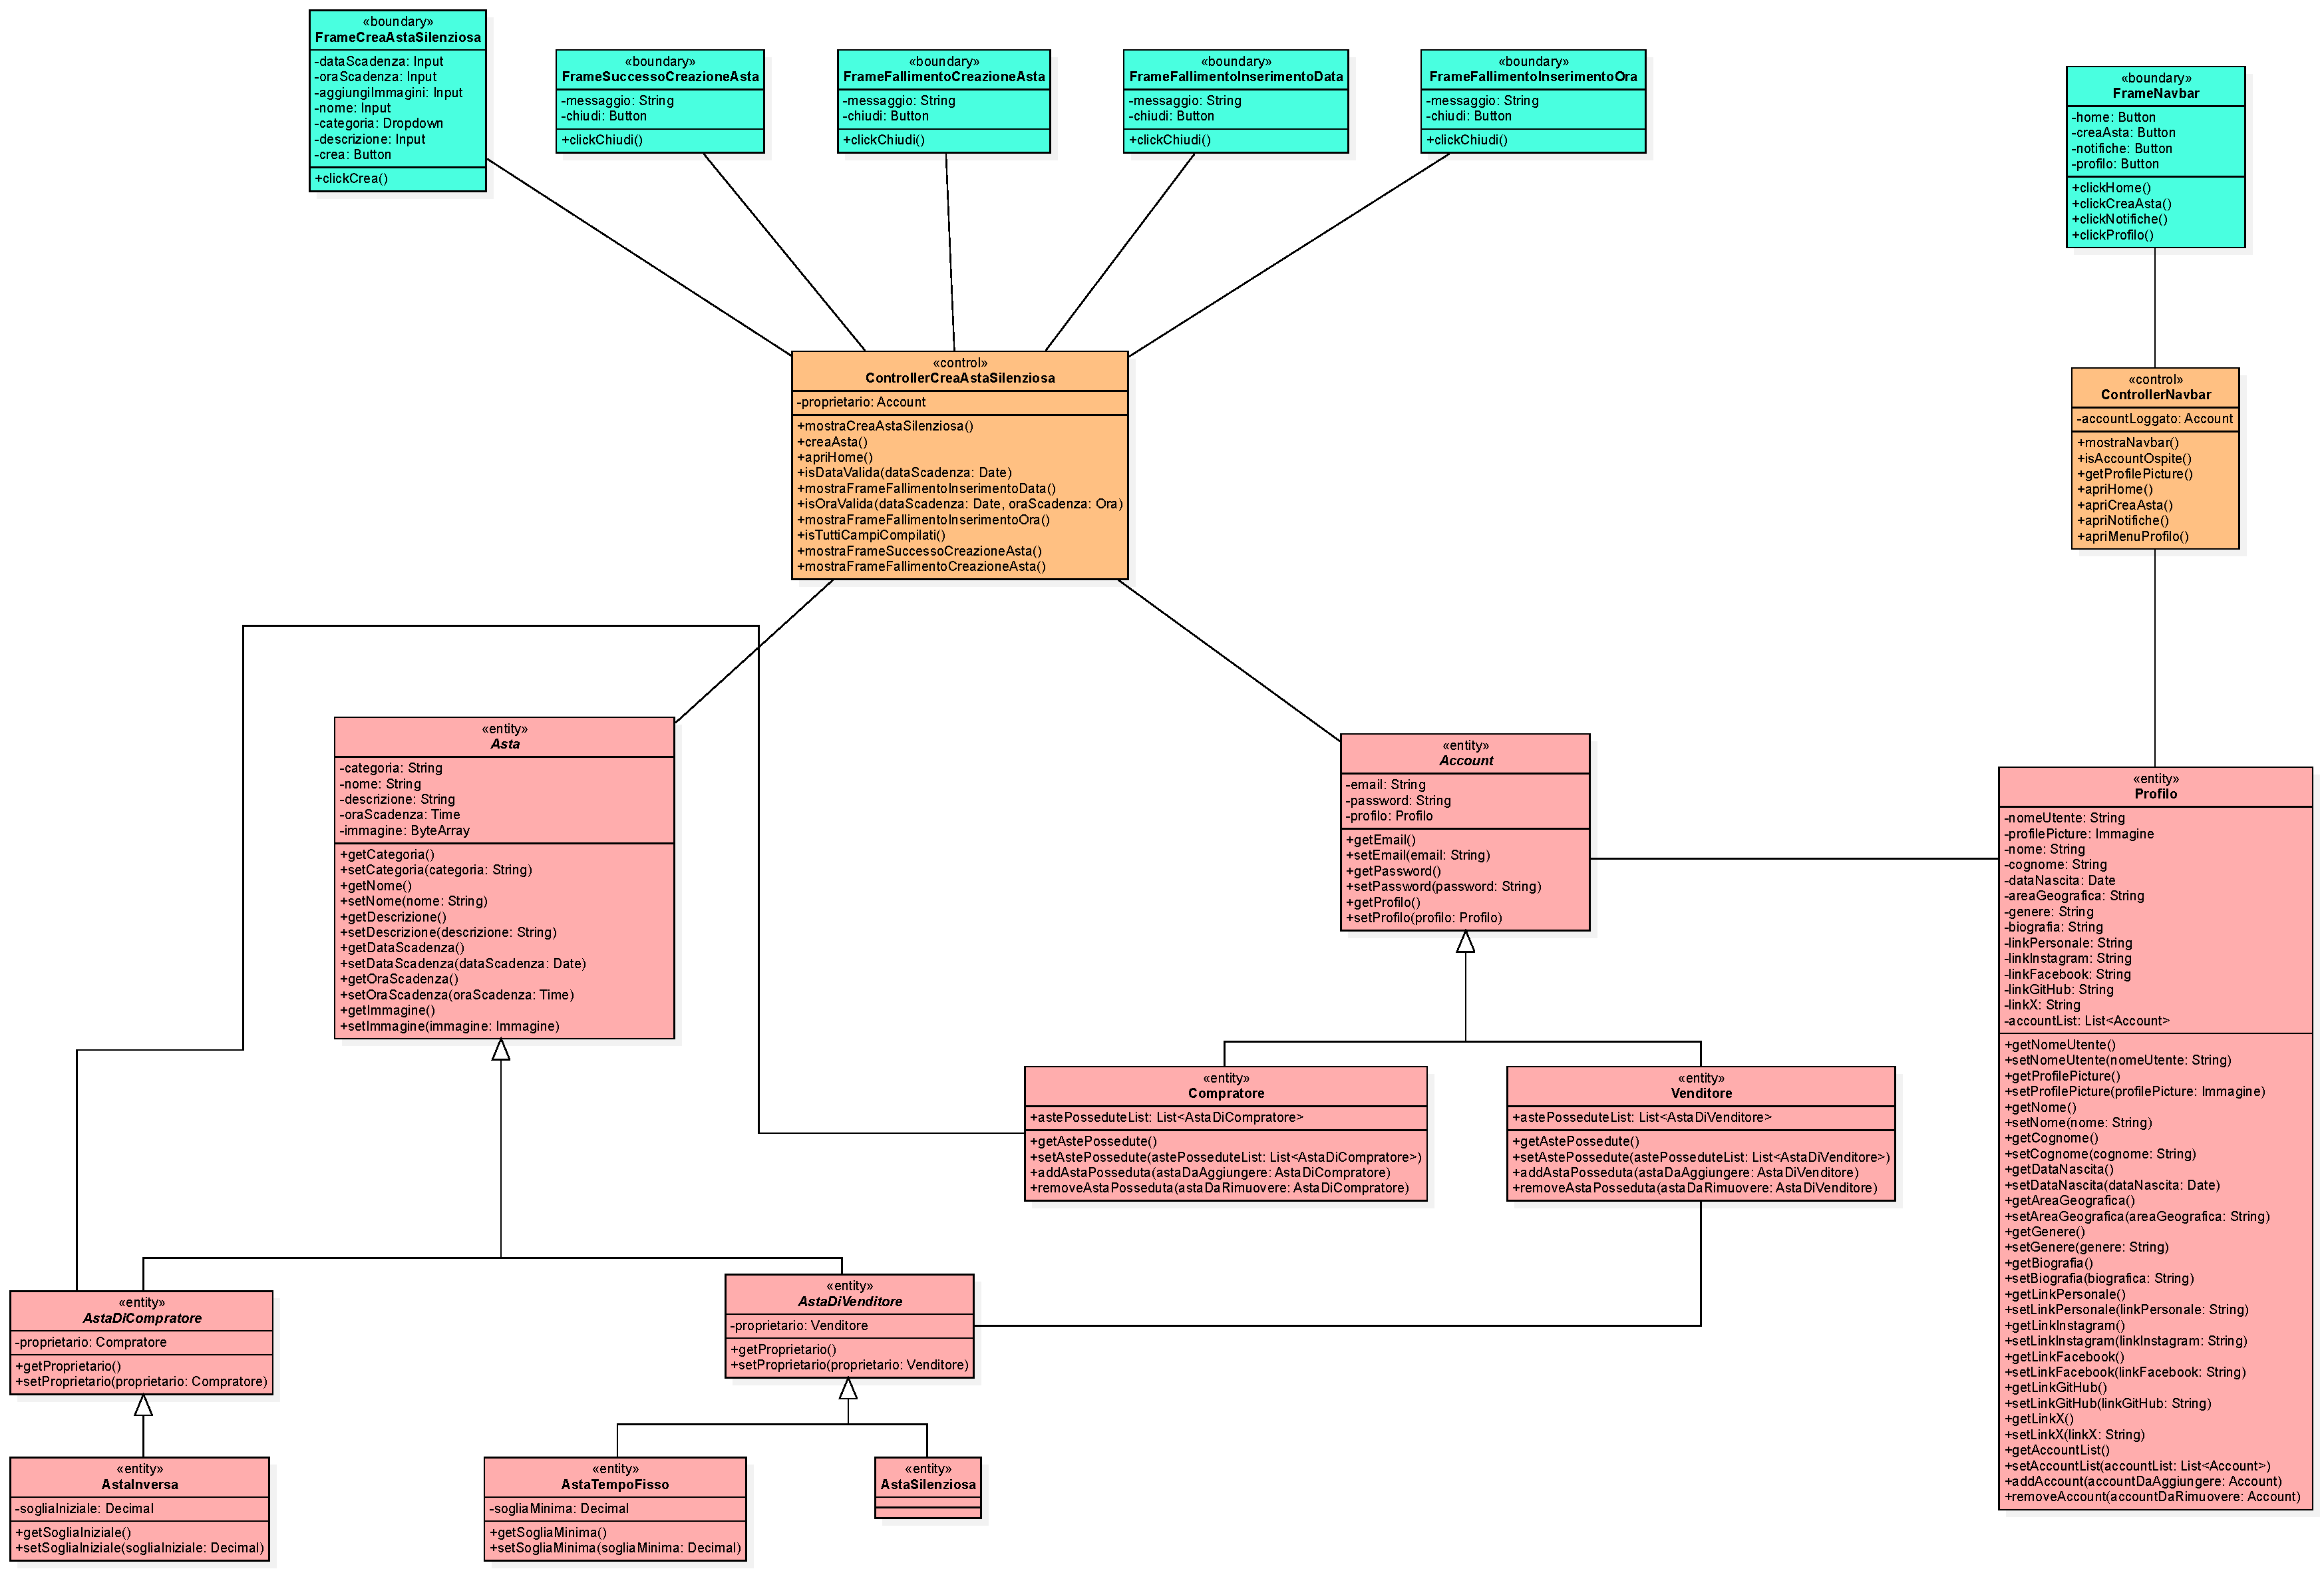
\includegraphics[width=1\linewidth]{Immagini/Diagrammi/Class Diagram/Venditore e compratore/CreaAstaSilenziosa.pdf}
                \caption{Crea un'asta silenziosa}
            \end{figure}
            
            \begin{figure}[htbp!]
                \centering
                    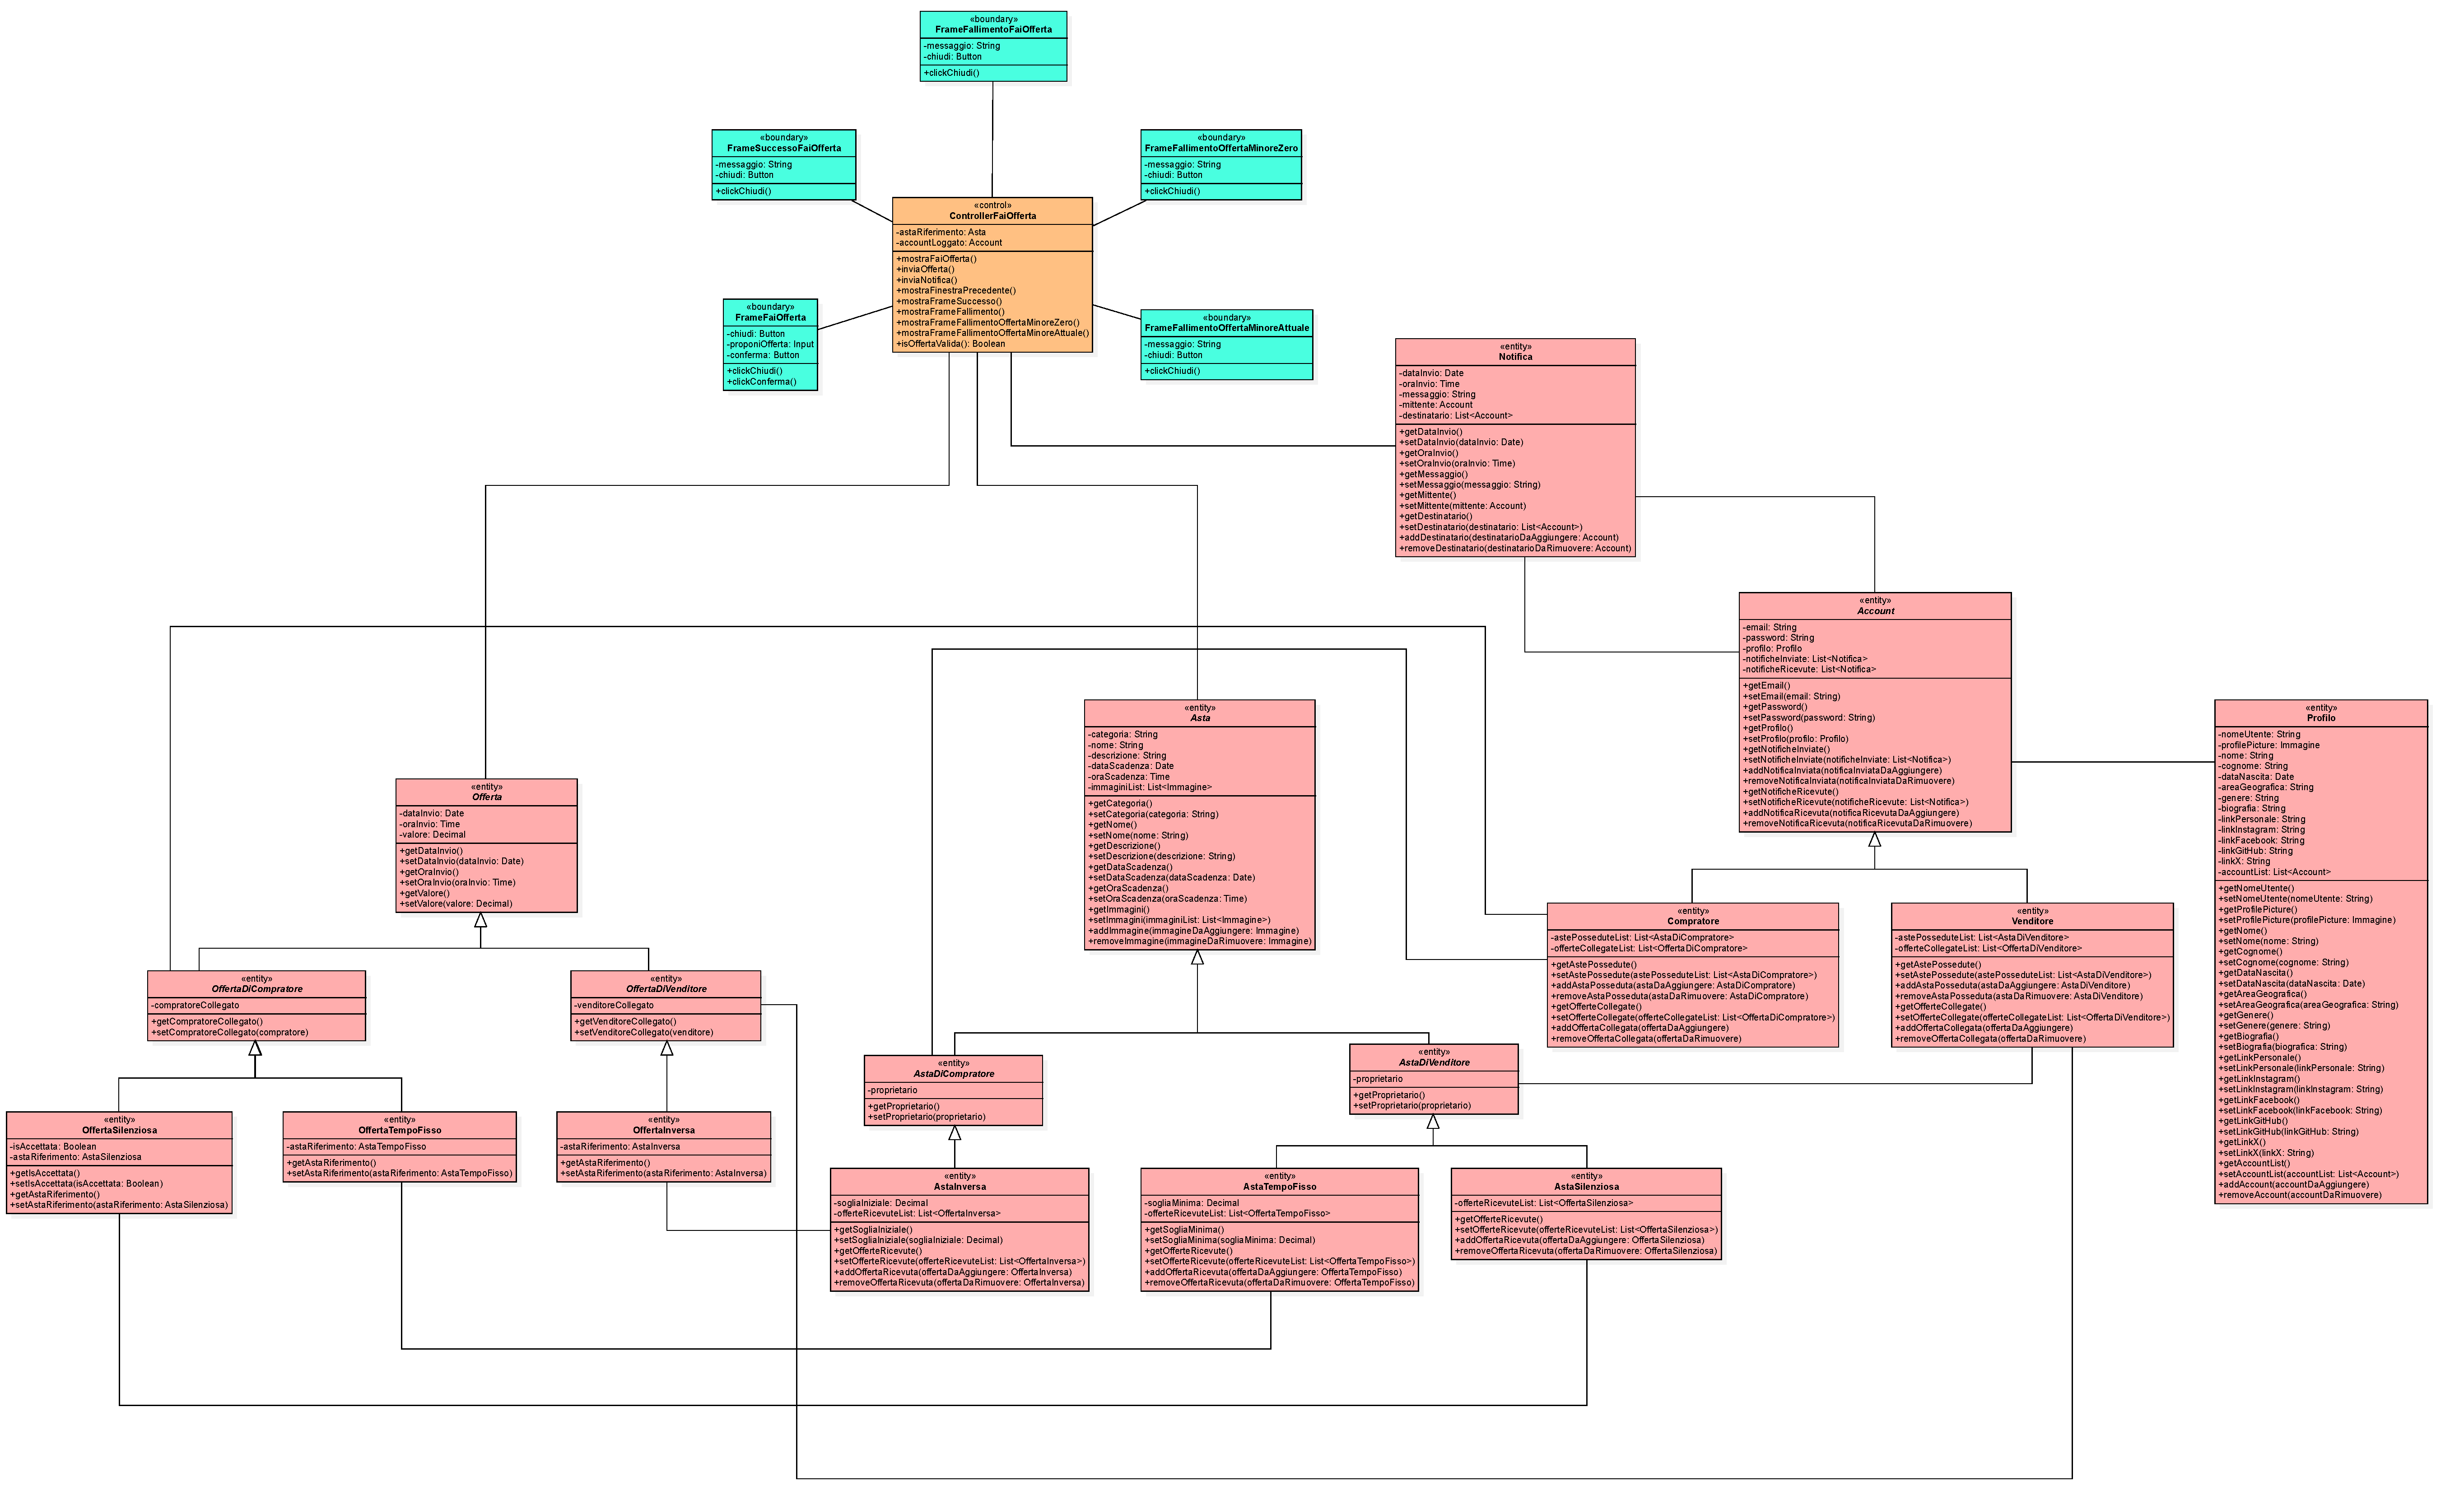
\includegraphics[width=1\linewidth]{Immagini/Diagrammi/Class Diagram/Venditore e compratore/FaiOfferta.pdf}
                \caption{Fai un'offerta}
            \end{figure}

    \clearpage
        
    \section{Dizionario delle classi}
        \begin{longtable}{|C{3.5cm}|L{11.2cm}|}
            \hline
            \multicolumn{1}{|c|}{\cellcolor{head}\textbf{Classe}} & \multicolumn{1}{c|}{\cellcolor{head}\textbf{Descrizione}}\\  
            \hline
                Account &
                L'account raccoglie le informazioni necessarie per permettere ad un utente dell'applicazione di effettuare l'accesso alla stessa. Esso può essere di due tipologie: compratore e venditore.\\
            \hline
                Venditore &
                Un account di tipo venditore è un account che rappresenta un utente che utilizza l'applicazione per vendere i propri beni o servizi ad altri utenti.\\
            \hline
                Compratore &
                Un account di tipo compratore è un account che rappresenta un utente che utilizza l'applicazione per acquistare beni o servizi da altri utenti.\\
            \hline
                Profilo &
                Il profilo concentra le informazioni di natura personale che riguardano l'utente registrato. Esso è condiviso tra l'account compratore e venditore di uno stesso utente.\\
            \hline
                Notifica &
                Una notifica è un messaggio che viene recepito da un utente; ciò avviene quando un'asta alla quale ha partecipato si è conclusa (ed eventualmente vinta), la sua offerta è stata accettata in un'asta silenziosa, o un'asta creata ha ricevuto un'offerta da un'utente.\\
            \hline
                Asta &
                Un'asta è un annuncio di compravendita di un bene o un servizio e che raccoglie tutte le informazioni che riguardano l'articolo e chi ha pubblicato questo annuncio. Anche questa può essere di tipo compratore o venditore.\\
            \hline
                Asta di compratore &
                Un'asta di tipo compratore è un'asta nella quale il compratore richiede a dei venditori di fornirgli un bene o un servizio. Essa è di un'unica tipologia, ossia un'asta inversa.\\
            \hline
                Asta di venditore &
                Un'asta di tipo venditore è un'asta nella quale il venditore fornisce a dei compratori un bene o un servizio da essi richiesto. Essa può essere di due tipologie, ossia un'asta a tempo fisso o un'asta silenziosa.\\
            \hline
                Asta a tempo fisso &
                Un'asta a tempo fisso è un'asta nella quale si stabilisce una data di fine, entro la quale i compratori possono fare delle offerte al rialzo, e una soglia minima da raggiungere. Quando sopraggiunge la data stabilita, la persona che ha offerto la cifra più alta si aggiudica l'asta. Se non c'è stata nessuna offerta o non si è raggiunta la soglia minima entro il tempo limite, allora l'asta è dichiarata fallita.\\
            \hline
                Asta silenziosa &
                Un'asta silenziosa è un'asta nella quale si stabilisce una data di fine, entro la quale i compratori possono fare offerte al rialzo. Gli offerenti non possono però vedere l'offerta attuale più alta, e quindi dovranno offrire alla cieca. Quando sopraggiunge la data stabilita, la persona della quale l'offerta è stata accettata si aggiudica l'asta. Se non c'è stata nessuna offerta o nessuna offerta è stata accettata entro il tempo limite, allora l'asta è dichiarata fallita.\\
            \hline
                Asta inversa &
                Un'asta inversa è un'asta nella quale si stabilisce una data di fine, entro la quale i venditori possono fare offerte al ribasso, e una soglia massima da cui partire. Quando sopraggiunge la data stabilita, la persona che ha offerto la cifra più bassa si aggiudica l'asta. Se non c'è stata nessuna offerta entro il tempo limite, allora l'asta è dichiarata fallita.\\
            \hline
                Offerta &
                Un'offerta è una somma di denaro che l'utente può inviare ad un'asta con lo scopo di aggiudicarsela.\\
            \hline
                Offerta di compratore &
                Un'offerta che viene inviata da un account compratore.\\
            \hline
                Offerta di venditore &
                Un'offerta che viene inviata da un account venditore.\\
            \hline
                 Offerta a tempo fisso &
                Un'offerta che viene inviata da un account compratore ad un'asta a tempo fisso.\\
            \hline
                Offerta silenziosa &
                Un'offerta che viene inviata da un account compratore ad un'asta silenziosa.\\
            \hline
                Offerta inversa &
                Un'offerta che viene inviata da un account venditore ad un'asta inversa.\\
            \hline
        \end{longtable}
        
    \section{Dizionario delle associazioni}
        \begin{longtable}{|C{3.5cm}|L{11.2cm}|}
            \hline
                \multicolumn{1}{|c|}{\textbf{Associazione}} &
                \multicolumn{1}{c|}{\textbf{Descrizione}}\\            
            \hline
                Mittente &
                Associazione tra Account e Notifica. Quando viene inviata una notifica, essa conserva l'utente che ha effettuato l'azione che ha innescato l'invio. Una notifica ha un solo mittente, ma un mittente può essere responsabile di più notifiche.\\
            \hline
                Destinatario &
                Associazione tra Account e Notifica. Quando viene inviata una notifica, essa conserva l'utente al quale deve essere mandata per sapere a chi arrivare. Una notifica ha uno o più destinatari, e un destinatario può ricevere più notifiche.\\
            \hline
                Possiede &
                Associazione tra Account e Profilo. Quando viene creato un account, esso viene collegato ad un profilo. Un account è collegato ad un solo profilo, e un profilo è collegato al più a due account, ossia uno di tipo compratore e uno di tipo venditore.\\
            \hline
                È associata a &
                Associazione tra Notifica e Asta. Quando viene inviata una notifica, essa conserva l'asta relativa all'evento che ha causato l'invio, così che l'utente possa raggiungere velocemente l'asta attraverso la notifica. Una notifica è associata ad una sola asta, ma un'asta è associata a più notifiche.\\
            \hline
                Possiede &
                Associazione tra Venditore e Asta di venditore. Un venditore può creare un'asta per la vendita di un bene o servizio e ne diventa il possessore e gestore. Un'asta è quindi associata ad un solo venditore, ma un venditore può creare più aste.\\
            \hline
                È collegato a &
                Associazione tra Venditore e Offerta di venditore. Quando viene inviata un'offerta dal venditore, essa conserva il suo offerente così che si possa risalire ad esso nell'elenco delle offerte dell'asta. Un'offerta è collegata ad un solo venditore, ma un venditore può inviare più offerte.\\
            \hline
                Possiede &
                Associazione tra Compratore e Asta di compratore. Un compratore può creare un'asta per l'acquisto di un bene o servizio e ne diventa il possessore e gestore. Un'asta è quindi associata ad un solo compratore, ma un compratore può creare più aste.\\
            \hline
                È collegato a &
                Associazione tra Compratore e Offerta di compratore. Quando viene inviata un'offerta dal compratore, essa conserva il suo offerente così che si possa risalire ad esso nell'elenco delle offerte dell'asta. Un'offerta è collegata ad un solo compratore, ma un compratore può inviare più offerte.\\
            \hline
                Si riferisce a &
                Associazione tra Offerta a tempo fisso e Asta a tempo fisso. Ogni offerta è collegata alla relativa asta. In particolare, ogni offerta è relativa ad una sola asta e ogni asta è collegata a più offerte.\\
            \hline
                Si riferisce a &
                Associazione tra Offerta silenziosa e Asta silenziosa. Ogni offerta è collegata alla relativa asta. In particolare, ogni offerta è relativa ad una sola asta e ogni asta è collegata a più offerte.\\
            \hline
                Si riferisce a &
                Associazione tra Offerta inversa e Asta inversa. Ogni offerta è collegata alla relativa asta. In particolare, ogni offerta è relativa ad una sola asta e ogni asta è collegata a più offerte.\\
            \hline
        \end{longtable}

    \clearpage
    
    \section{Sequence Diagram}
        Il diagramma di sequenza rappresenta i processi e gli oggetti coinvolti e la sequenza dei messaggi scambiati necessari per adempiere ad una funzionalità. \\
        Le interazioni sono disposte lungo un'asse temporale per dare un'idea dell'ordine di avvicendamento dei messaggi.
        
        \begin{figure}[htbp!]
        \centering
            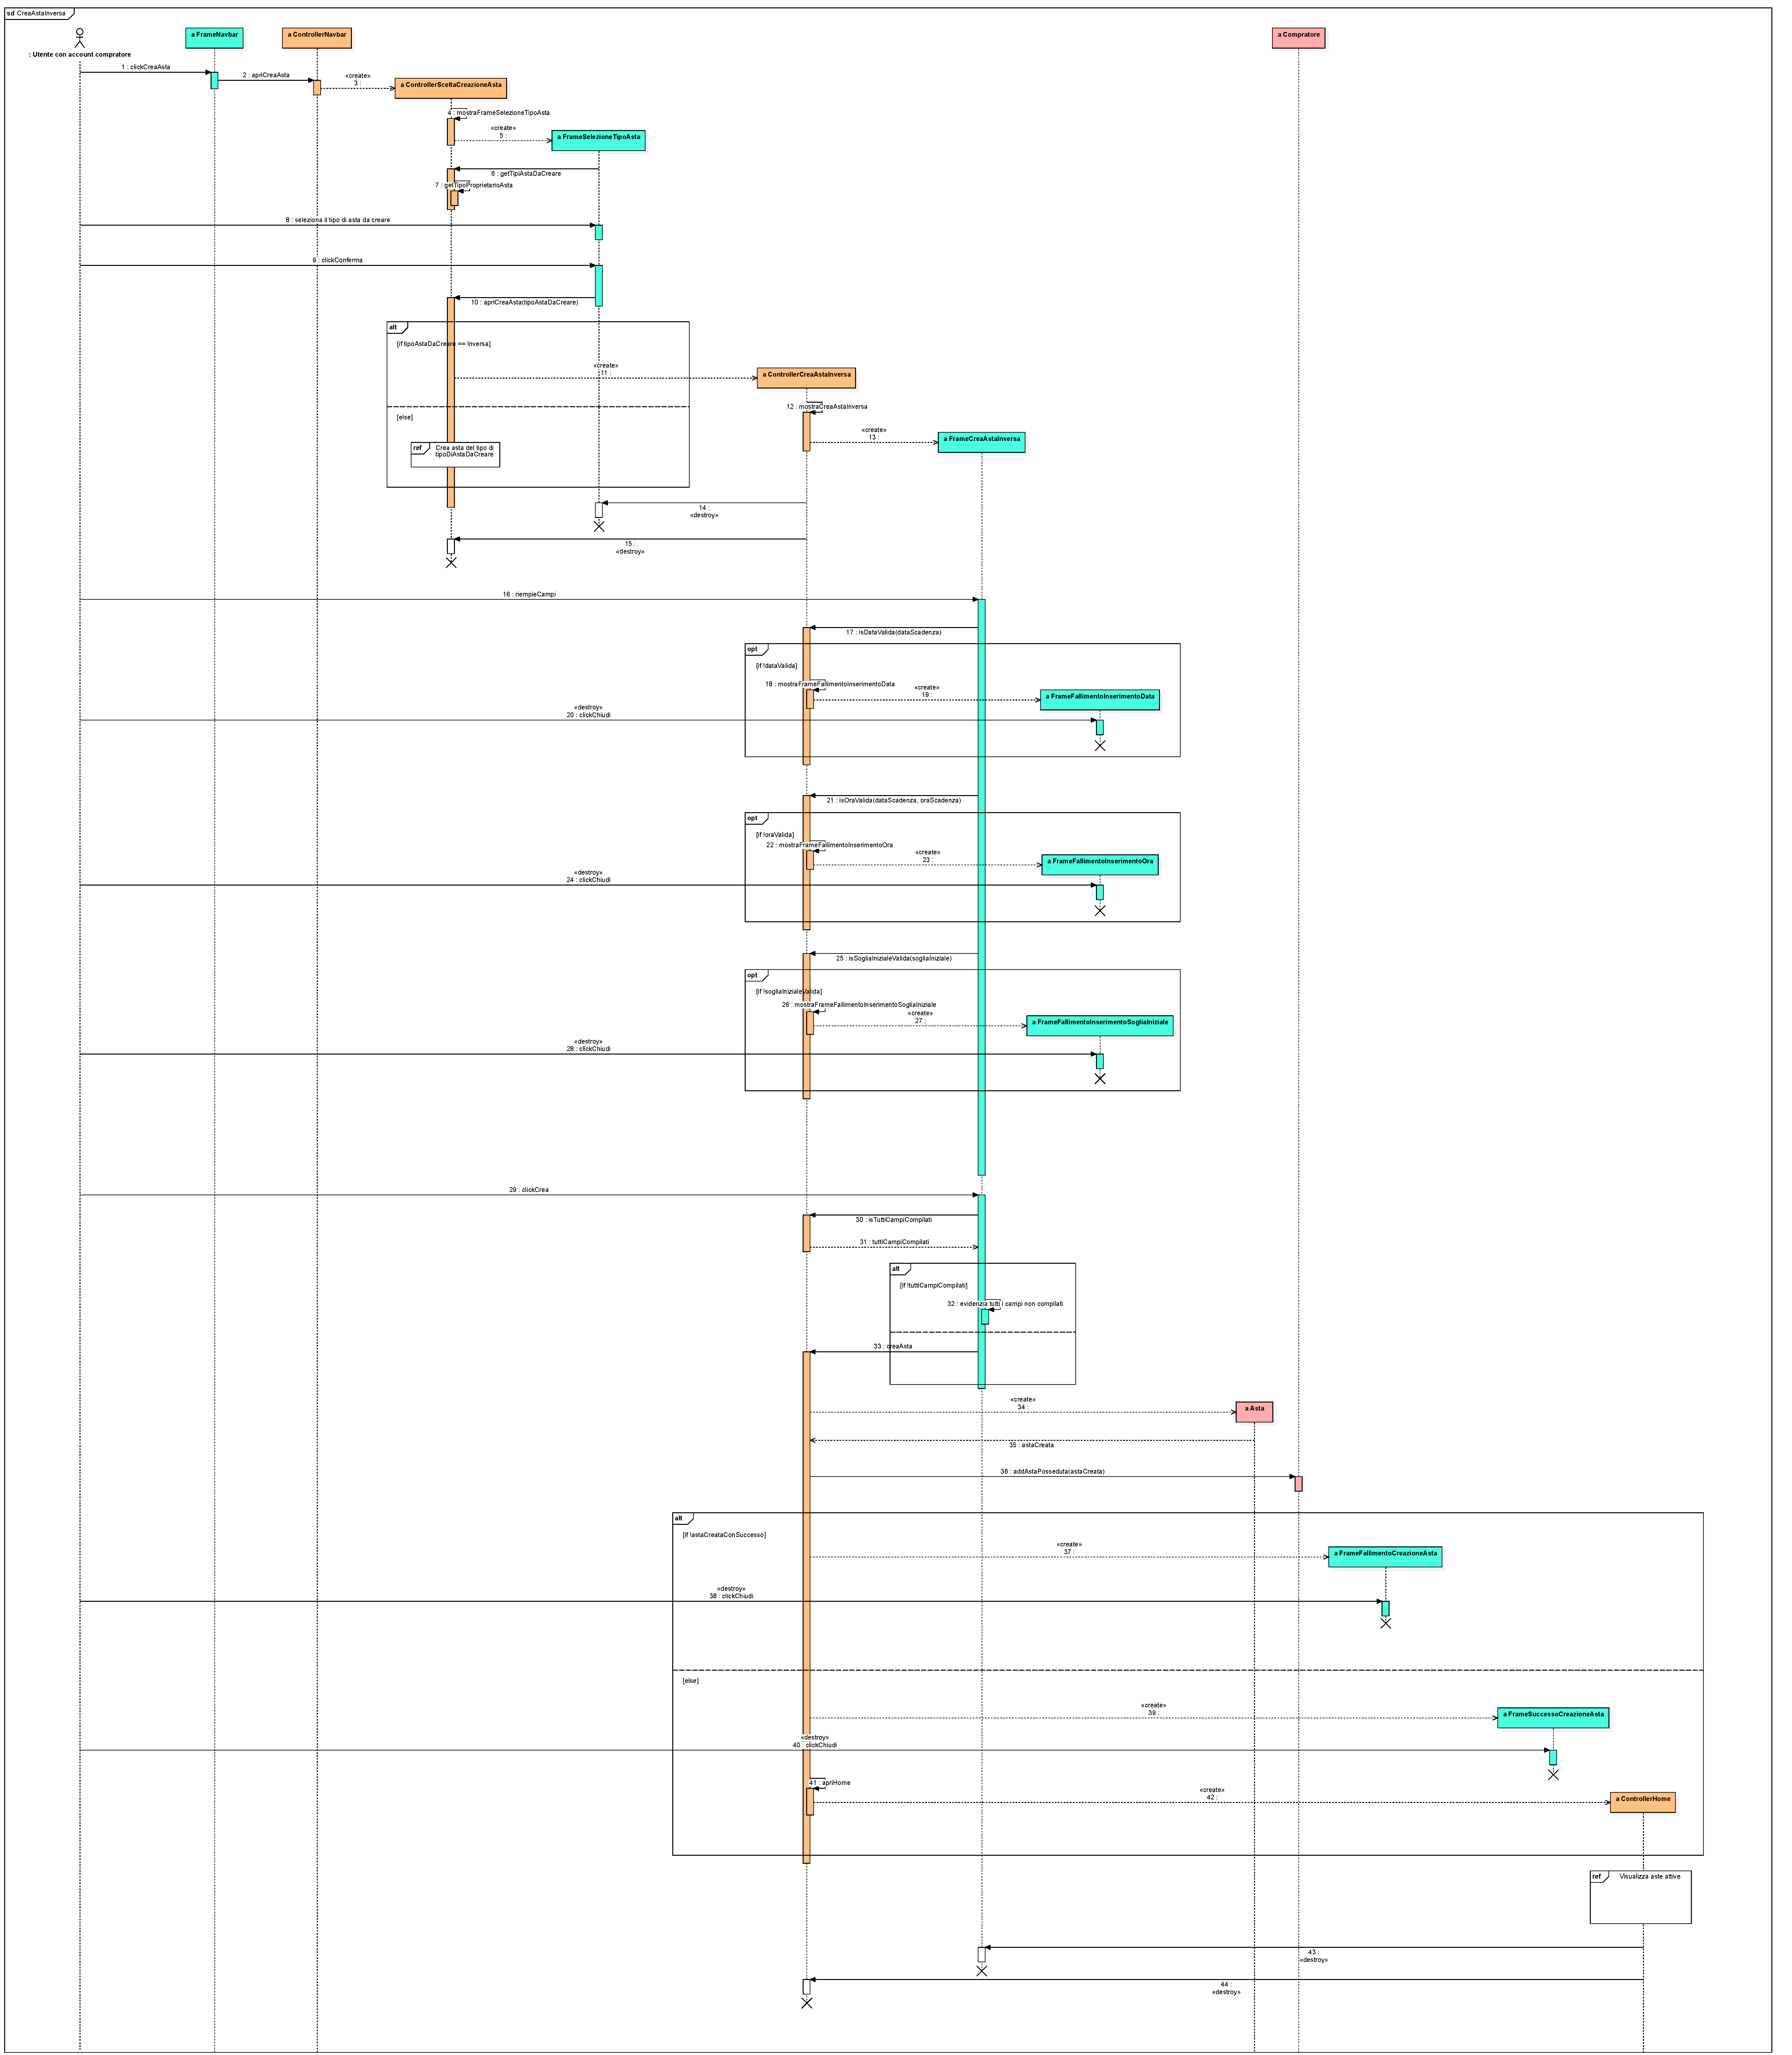
\includegraphics[width=1\linewidth]{Immagini/Diagrammi/Sequence Diagram/CreaAstaInversa.pdf}
        \caption{Sequence Diagram creazione asta inversa}
        \end{figure}

        \begin{figure}[htbp!]
        \centering
            \includegraphics[width=1\linewidth]{Immagini/Diagrammi/Sequence Diagram/AccettaOffertaSilenziosa.pdf}
        \caption{Sequence Diagram accetta offerta per un'asta silenziosa}
        \end{figure}

    \clearpage
    
    \section{Statechart Diagram}
        Il diagramma degli stati consente di rappresentare gli aspetti dinamici di un sistema, in particolare per l'interfaccia utente. \\
        Presenta quindi una serie di stati che il sistema attraversa (come una macchina a stati finiti), le azioni che comportano una transizione da uno stato all'altro, e le condizioni da rispettare affinché la transizione possa avvenire.

            \begin{figure}[htbp!]
            \centering
                \includegraphics[width=1\linewidth]{Immagini/Diagrammi/Statechart Diagram/CreaAstaInversa.pdf}
            \caption{Statechart Diagram creazione asta inversa}
            \end{figure}
            
            \begin{figure}[htbp!]
            \centering
                \includegraphics[width=1\linewidth]{Immagini/Diagrammi/Statechart Diagram/AccettaOffertaSilenziosa.pdf}
            \caption{Statechart Diagram accetta offerta per un'asta silenziosa}
            \end{figure}
    %PDF DI RIFERIMENTO: 06_System Design.pdf + DesignPractices.pdf, 08_Architetture Software.pdf, 08_Architetture.pdf, XX-REST-APIs.pdf

\chapter{System Design}
    La progettazione del sistema è un insieme di scelte effettuate dall'ingegnere del software per la trasformazione del modello di analisi nel modello di design del sistema. \\
    Vengono qui definiti gli obiettivi di progettazione del software, l'architettura del sistema (il quale viene decomposto in più sottosistemi realizzabili da differenti squadre di sviluppatori) e le strategie di creazione del sistema.

    \section{Architettura e criteri di progettazione}
        L'architettura di un software è la struttura del sistema, che comprende gli elementi del software, le proprietà visibili all'esterno di tali elementi, e le relazioni tra di essi. \\
        Sulla base delle richieste avanzate dagli utenti, ovvero di un’applicazione \textbf{portabile}, \textbf{facile da usare} e \textbf{rapida}, si ritiene che i criteri di progettazione sui quali bisogni focalizzarsi siano \textbf{bassi tempi di risposta (bassa latenza)}, \textbf{basso consumo di memoria}, \textbf{alta portabilità e modificabilità}. \\
        Per soddisfare tali requisiti qualitativi, il sistema deve essere suddiviso in diversi moduli tali che tra essi sussistano un'\textbf{alta coesione} e un \textbf{basso accoppiamento}. \\
        Si è optato, in questo sistema, per un'\textbf{architettura client-server a due livelli con modello client leggero}. \\
        Si desidera ora evidenziare i criteri di progettazione definiti che hanno portato a questa decisione:
        \begin{itemize}
            \item La coesione è una misura di quanto siano fortemente relate e mirate le responsabilità, cioè i servizi offerti da un modulo; ciò permetterà di ottenere un’alta manutenibilità del codice e focalizzare i cambiamenti in interventi mirati e precisi. \\
            Per ottenere un'alta coesione, si è optato per una architettura client-server, nella quale ogni modulo adempie ad una funzione ben precisa e le cui classi collaborano per lo stesso fine. \\
            L'architettura client-server è una architettura distribuita, ove un sottosistema "servitore" offre servizi e dati ad altri sottosistemi "cliente", i quali sono responsabili dell'interazione con l'utente. \\
            I client chiamano il server richiedendo un servizio e ad essi viene restituito il risultato; questa chiamata è possibile poiché i client conoscono le interfacce del server, ma non è vero il viceversa.
            \item L’accoppiamento è una misura su quanto fortemente un modulo sia dipendente da altri. \\
            Un basso accoppiamento permetterà il riutilizzo dei moduli nonché una facilitazione nella modifica dello stesso, senza che le modifiche possano avere conseguenze inaspettate su altri moduli. \\
            Per ottenere un basso accoppiamento, si è scelto di seguire la legge di Demetra, spingendo al massimo l'incapsulamento.
            \item Il modello client leggero è l'alternativa al modello client pesante in un'architettura client-server a doppio legame. \\
            In questo modello, il client si occupa solamente dell'interfaccia e l'interazione con l'utente, e quindi può essere eseguito su gran parte dei dispositivi, anche con modeste prestazioni. \\
            Lo svantaggio di tale scelta è che pone maggior carico di elaborazione sia sul server, che si occupa della logica dell'applicazione e dell'immagazzinamento dei dati, sia sulla rete.
        \end{itemize}

    \section{Tecnologie adottate}
        Il client è un'applicazione per sistema operativo \textbf{Android}, scritta in linguaggio \textbf{Kotlin} e fa uso della libreria per la gestione delle immagini \textbf{Coil}. \\
        Il server si articola in:
        \begin{itemize}
            \item Un'applicazione \textbf{Java} salvata in un'immagine ed eseguita in un container del programma \textbf{Docker (Compose)}, installato su una macchina virtuale fornita da \textbf{AWS EC2}.
            \item Una base di dati relazionale \textbf{PostgreSQL}, al cui interno sono conservati tutti i dati dell'applicazione, eseguita anch'essa come immagine Docker sulla stessa macchina virtuale AWS EC2.
        \end{itemize}
        Le immagini sono archiviate nella macchina virtuale AWS EC2. \\
        Per lo scambio di messaggi tra client e server (attraverso le \textbf{REST API}), si utilizzano \textbf{Retrofit} su client e \textbf{Spring Framework} su server. \\

        \subsection{Android}
            \subsubsection{Cos'è Android? \cite{Wikipedia1}}
                Android è un sistema operativo gratuito ed open source, basato su una versione modificata del kernel Linux e di altri software open source. Creato originariamente per dispositivi touch come smartphone e tablet, è ora esteso a circa 2.5 miliardi di dispositivi \cite{Google1}, tra i quali anche smartwatch (Wear OS), smart TV (Android TV) e personal computer (questi ultimi utilizzano una versione modificata della distribuzione Gentoo Linux, chiamata Chrome OS, ma possono eseguire una macchina virtuale per utilizzare applicazioni Android). Il sistema operativo è correntemente sviluppato da Google.
            \begin{figure}[htbp!]
                \centering
                
\includegraphics[width=0.5\linewidth]{Immagini/System Design/Android.png}
                \caption{Logo di Android}
            \end{figure}
            \subsubsection{Perché Android?}
                Quasi tutti ormai posseggono uno smartphone. Ed essendo un sistema operativo così diffuso (conta circa il 69.94\% del mercato dei sistemi operativi per dispositivi mobili \cite{Statcounter1}) e disponibile su una grande varietà di dispositivi, Android è la scelta giusta per rendere l'applicazione disponibile quasi ovunque ed accessibile a chiunque.
                
        \subsection{Kotlin}
            \subsubsection{Cos'è Kotlin? \cite{Wikipedia2}}
                Kotlin è un linguaggio di programmazione multi-piattaforma, staticamente e fortemente tipizzato con inferenza di tipo, general purpose, multi-paradigma (orientato agli oggetti, imperativo, funzionale). Sviluppato da JetBrains, Kotlin è realizzato per essere interscambiabile con Java, poiché è interpretato da una macchina virtuale Java (JVM) che utilizza la libreria di classi Java standard. Ha pian piano soppiantato l'utilizzo di Java per la realizzazione di applicazioni Android ed è diventato nel 2019 il linguaggio primario e consigliato da Google per la realizzazione di esse.
            \begin{figure}[htbp!]
                \centering
                
\includegraphics[width=0.5\linewidth]{Immagini/System Design/Kotlin.png}
                \caption{Logo di Kotlin}
            \end{figure}
            \subsubsection{Perché Kotlin? \cite{JetBrains1}}
                Circa il 50\% degli sviluppatori Android utilizza Kotlin (Java ricopre il 30\%), e il 70\% di essi afferma che lo sviluppo in Kotlin li abbia resi più produttivi. Lo sviluppo con Kotlin consente di beneficiare di:
                \begin{itemize}
                    \item Minore quantità di codice con conseguente maggiore leggibilità;
                    \item Minore quantità di errori comuni che potrebbero comportare il crash delle applicazioni (ad esempio la gestione della nullità dei riferimenti \cite{JetBrains2});
                    \item Supporto per la libreria Jetpack Compose per la costruzione di interfaccia utente delle applicazioni;
                    \item Supporto per lo sviluppo multi-piattaforma, poiché le librerie Kotlin possono essere utilizzabili anche per lo sviluppo di app iOS, desktop e web;
                    \item Maturità del linguaggio e dell'ambiente di sviluppo, continuamente migliorati e supportati;
                    \item Interoperabilità con Java, consentendo in iniettare codice Java in quello Kotlin e di utilizzare librerie di Java con Kotlin;
                    \item Semplicità e facilità di apprendimento ed utilizzo.
                \end{itemize}
                 
        \subsection{Coil}
            \subsubsection{Cosè Coil?}
                Coil (COroutine Image Loader) è una libreria per il caricamento delle immagini nelle app Android, scritta interamente in Kotlin, che permette di rendere semplici, rapidi ed indolori la visualizzazione delle immagini sull'interfaccia e la gestione in memoria delle stesse.
            \begin{figure}[htbp!]
                \centering
                
\includegraphics[width=0.5\linewidth]{Immagini/System Design/Coil.png}
                \caption{Logo di Coil}
            \end{figure}
            \subsubsection{Perché Coil? \cite{Github1}}
                Coil sfrutta le Coroutine Kotlin per assolvere al suo ruolo in maniera asincrona. Coil è:
                \begin{itemize}
                    \item Rapido, grazie a numerose operazioni di ottimizzazione quali cache in memoria e su archiviazione, sotto-campionamento delle immagini in memoria, gestione automatica delle richieste di pausa e cancellazione della visualizzazione ed altro;
                    \item Leggero, poiché aggiunge la quantità minima di metodi possibili per svolgere le sue funzioni;
                    \item Facile da usare, poiché sfrutta la semplicità di Kotlin e codice boilerplate minimale;
                    \item Moderno, perché sfrutta le più moderne librerie di Kotlin quali Coroutine, OkHttp, Okio, e Lifecycle AndroidX.
                \end{itemize}
                
        \subsection{Java}
            \subsubsection{Cos'è Java?}
                Java è un linguaggio di programmazione staticamente e fortemente tipizzato, general purpose, multi-paradigma (orientato agli oggetti, imperativo, funzionale). Sviluppato da Oracle, in precedenza Sun Microsystems, è un linguaggio interpretato e compilato. Il codice sorgente è compilato in un linguaggio intermedio chiamato bytecode che viene interpretato da una macchina virtuale Java (JVM).  Java è presente su miliardi di dispositivi in tutto il mondo.
            \begin{figure}[htbp!]
                \centering
                
\includegraphics[width=0.15\linewidth]{Immagini/System Design/Java.png}
                \caption{Logo di Java}
            \end{figure}
            \subsubsection{Perché Java?}
                Il fatto che Java sia un linguaggio eseguito su macchina virtuale comporta:
                \begin{itemize}
                    \item Sicurezza, perché ogni programma è isolato e ogni comunicazione con l'esterno è controllata dalla JVM, impedendo l'esecuzione di codice malizioso;
                    \item Portabilità, poiché il codice viene trasformato in un codice universalmente comprensibile da tutte le implementazioni della JVM sui vari dispositivi (PC, dispositivi mobili, dispositivi specializzati, server, workstation...);
                \end{itemize}
                Il linguaggio è anche open source e ampiamente utilizzato da milioni di sviluppatori nel mondo, e possiede una ricca libreria standard di funzioni per la realizzazione delle applicazioni. Infine, molti framework, tra i quali il selezionato Spring, si basano proprio su questo linguaggio.
                
        \subsection{Docker (Compose)}
            \subsubsection{Cos'è Docker (Compose)?}
                Docker è un insieme di servizi Platform as a Service (PaaS) che utilizza la virtualizzazione a livello di sistema operativo del kernel per eseguire programmi in ambienti isolati e distribuibili chiamati container, i quali sono gestiti dal Docker Engine \cite{Wikipedia5}. I container sono leggeri e al loro interno conterranno tutto il necessario per l'esecuzione del software, senza preoccuparsi di quale macchina sta eseguendo il Docker Engine. Questi container sono configurabili attraverso l'uso di file di configurazione appositi. Compose, inizialmente un add-on per la piattaforma Docker, è stato successivamente incluso al suo interno, e consente attraverso un singolo file YAML la gestione e la comunicazione reciproca di più container. I container sono un'istanza di un'immagine Docker, ossia un template di sola lettura che istruisce su come il container debba essere creato \cite{Docker1}.
            \begin{figure}[htbp!]
                \centering
                
\includegraphics[width=0.5\linewidth]{Immagini/System Design/Docker.png}
                \caption{Logo di Docker}
            \end{figure}
            \subsubsection{Perché Docker (Compose)?}
                Il successo di Docker è dovuto al rivoluzionario approccio allo sviluppo che esso promuove. Grazie a Docker, si può impacchettare all'interno di un'immagine Docker l'applicazione e tutto l'ambiente necessario alla sua esecuzione. L'immagine può essere caricata sulla repository centrale di Docker affinché chiunque possa accedervi, o comunque essere distribuita. Non bisogna quindi preoccuparsi di nulla: ogni container è isolato e contiene tutto ciò che è necessario, e non c'è bisogno di installare applicazioni oltre al Docker Engine, né gestire le librerie o le versioni dei linguaggi installati. Aggiornamenti dei software possono essere sempre rilasciati attraverso le immagini, e basta scaricarne la nuova versione e metterla in esecuzione sull'Engine per poter disporre degli ultimi strumenti. Permette anche di avere sulla stessa macchina più istanze in esecuzione di una stessa applicazione o servizio per favorire il bilanciamento del carico, la tolleranza al guasto e l'isolamento in caso di compromissione.
                
        \subsection{Google Cloud}
            \subsubsection{Cos'è Google Cloud?}
                Google Cloud Platform (GCP) è una suite di servizi di cloud computing offerta da Google che fornisce una enorme quantità di servizi cloud modulari, tra cui l'elaborazione, l'archiviazione dei dati, l'analisi dei dati e l'apprendimento automatico, insieme a una serie di strumenti di gestione. Esso è gestito con la stessa infrastruttura che Google utilizza internamente per i suoi prodotti per gli utenti finali. \cite{Wikipedia7} Nel contesto dell'applicazione DietiDeals24, sono stati utilizzati i servizi Artifact Registry per la conservazione delle immagini Docker, Cloud Build per la costruzione dei container a partire dalle immagini e Cloud Run per il deploy serverless del backend, Firebase per log e statistiche di utilizzo.
            \begin{figure}[htbp!]
                \centering
                
\includegraphics[width=0.5\linewidth]{Immagini/System Design/Google Cloud.png}
                \caption{Logo di Google Cloud}
            \end{figure}
            \subsubsection{Perché Google Cloud?}
                Google Cloud offre un'infrastruttura altamente scalabile, che consente alle aziende di crescere in modo efficiente. Possiede centri dati in tutto il mondo, garantendo bassa latenza ed alta disponibilità. Offre solide misure di sicurezza, tra cui crittografia dei dati, certificazioni di conformità e rilevamento avanzato delle minacce. Dispone di potenti strumenti di machine learning e AI che consentono analisi avanzate dei dati. Infine, con la tariffazione "pay-as-you-go", le aziende possono gestire i costi in modo efficace e pagare solo per ciò che utilizzano.

        \subsection{PostgreSQL}
            \subsubsection{Cos'è PostgreSQL? \cite{PostgreSQL1}}
                PostgreSQL è una potente base di dati relazionale gratuita ed open source che usa il linguaggio SQL standard ma non disdegnando delle aggiunte utili per conservare e scalare i carichi di dati più complessi (è gergalmente definito un "dialetto"). PostgreSQL ha una forte reputazione di RDBMS robusto, affidabile, estensibile. Esso è eseguibile su tutti i principali sistemi operativi e garantisce le proprietà ACID (atomicità, consistenza, isolamento, durabilità) per dati e transazioni. Inoltre fornisce anche utili add-on per estendere le capacità della base di dati. È disponibile sia attraverso riga di comando che GUI.
            \begin{figure}[htbp!]
                \centering
                
\includegraphics[width=0.2\linewidth]{Immagini/System Design/PostgreSQL.png}
                \caption{Logo di PostgreSQL}
            \end{figure}
            \subsubsection{Perché PostgreSQL?}
                PostgreSQL fornisce numerose funzionalità utili per lo sviluppo delle applicazioni, la protezione dell'integrità dei dati e la costruzione di ambienti tolleranti al guasto. Permette anche di scrivere procedure e funzioni procedurali in differenti linguaggi e per differenti linguaggi di programmazione (PL/pgSQL, PL/Tcl, PL/Perl, PL/Pyhton). Tra le funzionalità notevoli, si possono annoverare:
                \begin{itemize}
                    \item Supporto ad una vasta quantità di tipi di dato;
                    \item Funzionalità per il controllo dell'integrità dei dati;
                    \item Esecuzione concorrente e alte prestazioni;
                    \item Affidabilità e ripresa dal disastro;
                    \item Elevata sicurezza;
                    \item Ampia estensibilità;
                    \item Internazionalità e capacità di elaborazione testuale \cite{PostgreSQL1}; 
                    \item Supporto sempre gratuito;
                    \item Il linguaggio procedurale PL/pgSQL è pienamente compatibile con il linguaggio procedurale di altre basi di dati, facilitando eventuali future migrazioni \cite{Hevodata1}.
                \end{itemize}

        \subsection{REST API}
            \subsubsection{Cosa sono le REST API? \cite{IBM1}}
                Le REST API (REpresentational State Transfer Application Programming Interface) sono un'interfaccia di programmazione dell'applicazione che segue i princìpi REST, utilizzata per connettere tra loro componenti e applicazioni in un'architettura di microservizi. Le REST API sfruttano l'impalcatura del protocollo HTTP per poter permettere di effettuare tutte le principali operazioni sui dati attraverso i metodi HTTP, e i messaggi sono scambiati attraverso file JSON (ma anche XML o HTML).
            \subsubsection{Perché le REST API?}
                I sei princìpi REST sono un'interfaccia uniforme, il disaccoppiamento client-server, servizio senza stato, possibilità di utilizzo del meccanismo di cache, organizzazione del sistema a più livelli, ed esecuzione di codice su richiesta \cite{IBM1}. La realizzazione di applicazioni che comunicano attraverso REST API permette di spingere al massimo l'indipendenza tra i vari servizi, non rinunciando però ad una semplicità di fondo nella comunicazione, essendo il protocollo HTTP un protocollo maturo, quindi testato e funzionante, e strutturalmente semplice. Inoltre, la comunicazione attraverso file JSON (un formato comodo nella lettura sia per esseri umani che per calcolatori e uno dei formati di scambio dei dati più diffuso al mondo), ne permette la lettura da parte di moltissimi linguaggi di programmazione, ciascuno dei quali in possesso di strumenti di parsing di tale formato.

        \subsection{Retrofit}
            \subsubsection{Cos'è Retrofit?}
                Retrofit è un client HTTP type-safe per Android e Java sviluppato da Square. Semplifica il processo di interazione con i servizi web, consentendo agli sviluppatori di definire gli endpoint delle API mediante annotazioni e di eseguire le richieste di rete attraverso queste interfacce. Retrofit gestisce i dettagli delle richieste web, delle risposte e del parsing dei dati, facilitando l'integrazione delle API REST nelle applicazioni Android e Java.
            \begin{figure}[htbp!]
                \centering
                
\includegraphics[width=0.5\linewidth]{Immagini/System Design/Retrofit.png}
                \caption{Logo di Retrofit}
            \end{figure}
            
        \subsection{Spring Framework}
            \subsubsection{Cos'è Spring Framework?}
                Spring è un framework gratuito ed open source per applicazioni web scritte in Java. Inizialmente nato come alternativa al modello Enterprise JavaBeans di Java Enterprise Edition (ora Jakarta Enterprise Edition), le sue funzioni possono essere utilizzate da qualsiasi applicazione Java, e fornisce anche numerosi servizi aggiuntivi, che prendono il nome di Spring Boot, Spring Security, Spring Data, eccetera \cite{Wikipedia4}. Grazie a Spring, si possono realizzare delle REST API per la propria applicazione.
            \begin{figure}[htbp!]
                \centering
                
\includegraphics[width=0.5\linewidth]{Immagini/System Design/Spring.png}
                \caption{Logo di Spring}
            \end{figure}
            \subsubsection{Perché Spring Framework? \cite{Spoclearn1}}
                I punti forti di Spring sono:
                \begin{itemize}
                    \item Alta modularità e basso livello di dipendenze grazie al potente meccanismo di dependency injection, che promuove un basso accoppiamento, facilitando manutenzione e riusabilità;
                    \item  Ricco ecosistema, fornendo molti strumenti per ricoprire le varie necessità di sviluppo dell'applicazione;
                    \item Programmazione orientata all'aspetto, ossia permette di incapsulare le fasi più critiche dello sviluppo dell'applicazione, come la sicurezza e il tracciamento delle attività attraverso file di log;
                    \item Una community molto estesa e documentazione molto ampia;
                    \item Il supporto dello sviluppo orientato al test, assieme alla semplicità nella gestione delle dipendenza, contribuisce a migliori pratiche di test;
                    \item Flessibilità nella scelta di specifici componenti e moduli in base alle necessità del progetto.
                \end{itemize}
    %PDF DI RIFERIMENTO: 06_System Design.pdf + DesignPractices.pdf, 08_Architetture Software.pdf, 08_Architetture.pdf

\chapter{Object Design}
    La progettazione orientata agli oggetti è la fase di sviluppo del software nella quale si definisce il dettaglio implementativo dei vari sottosistemi. \\
    Tali sottosistemi devono soddisfare i requisiti non funzionali di performance, affidabilità e manutenibilità. Sono costruiti sulla base degli oggetti individuati nel dominio del problema, ai quali inevitabilmente saranno aggiunti nuovi oggetti per giungere alla soluzione. \\
    Le scelte adoperate hanno l'obiettivo di favorire il basso accoppiamento tra i sottosistemi e la manutenibilità, in modo da mantenere un'alta qualità interna del software.

    \section{Design Pattern}
        \subsection{Client}
            Il client possiede un'architettura con due strati: lo \textbf{strato della UI} e lo \textbf{strato dei dati}. \\
            Nel complesso, è un ibrido tra il pattern \textbf{MVVM} (Model-View-ViewModel) e \textbf{MVC} (Model-View-Controller).

            \begin{figure}[htbp!]
                \centering
                \includegraphics[width=0.45\linewidth]{Immagini/Object Design/ArchitetturaClient.pdf}
                \caption{Schema dell'architettura adottata (client)}
            \end{figure}
            
            \begin{itemize}
                \item Lo strato della UI comprende \textbf{View}, \textbf{StateHolder} (che mantengono i dati sullo stato della View, come i \textbf{ViewModel}) e \textbf{Controller} e si occupa di gestire l'interfaccia e l'interazione con l'utente.
                    \begin{itemize}
                        \item Le \textit{View} sono dei file .XML che utilizzano degli schemi definiti da Android per la creazione dell'interfaccia utente. Inoltre, grazie al View binding, per ogni vista viene generata una classe Java che contiene riferimenti a tutti gli elementi della vista per poter interagire con essa. Esse interagiscono con il Controller per chiamare i metodi che gestiscono l'interazione con l'utente.
                        \item I \textit{ViewModel} sono delle classi che hanno il compito di mantenere i dati che devono essere mostrati sulla UI. L'utilizzo del ViewModel è essenziale per poter mantenere i dati anche in caso di cambiamenti dello stato dell'applicazione, come rotazioni dello schermo o riduzione ad attività in secondo piano. I ViewModel, che nella architettura MVVM interagiscono direttamente con il Model e si interpongono tra quest'ultimo e la View, eseguono anche operazioni sui dati, come il recupero dei dati paginati da mostrare sullo schermo e la validazione dei dati inseriti dall'utente.
                        \item L'aggiunta del \textit{Controller} è ciò che rende ibrida questa architettura. Il Controller si interpone tra ViewModel e View per separare i compiti che riguardano il conservare e il convalidare i dati della vista (affidati al ViewModel) da altre operazioni, come appunto le risposte all'interazione con l'utente, la creazione di messaggi di errore, e l'invio di richieste non relative a dati da mostrare, come ad esempio l'autenticazione. Inoltre esso funge da osservatore ai dati che sono presenti nel ViewModel e, in caso di mutazione, provvede ad aggiornare la vista con tali nuovi dati.
                    \end{itemize}
                \item Lo strato dei dati è rappresentato dal \textbf{Model} e il suo ruolo è comunicare con le fonti di dati, siano esse esterne (come basi di dati) che locali (come cache o basi di dati interne). Il Model, a sua volta, è organizzato secondo il pattern \textbf{Repository}, con tre sottostrati: \textbf{Repository}, \textbf{Service} e \textbf{ServiceImpl}.
                    \begin{itemize}
                        \item Le classi \textit{Repository} rappresentano una enumerazione delle operazioni che la logica dell'applicazione può effettuare sui dati, chiamando poi attraverso le interfacce Service i metodi che svolgono l'effettivo lavoro sui dati.
                        \item Le classi \textit{Service} rappresentano una interfaccia che astrae queste operazioni sui dati. In questo caso, esse rappresentano una interfaccia di metodi che verranno utilizzati per la creazione di richieste HTTP da inviare agli endpoint del backend.
                        \item Le classi \textit{ServiceImpl} rappresentano dei metodi concreti - implementati dalla libreria Retrofit - che, sulla base delle annotazioni e i parametri inseriti nelle interfacce dei metodi di Service, creeranno la giusta richiesta HTTP da inviare al backend.
                    \end{itemize}
            \end{itemize}
    
        \subsection{Resource Server}
            L'architettura adottata per il sottosistema \textbf{Resource Server} (da qui in avanti chiamato semplicemente \textbf{Server}) è un'architettura di tipo \textbf{esagonale}. L'obiettivo di tale architettura è di definire una \textbf{separazione netta} tra la business logic del dominio (anche detto \textit{domain layer}) e tutto ciò che sono i fattori esterni, ovvero il layer di interfaccia con l'utente (anche detto \textit{application layer}) e il layer di persistenza (anche detto \textit{infrastracture layer}), attraverso una serie di interfacce ben definite. \\
            L'obiettivo di tale scelta è quello di migliorare la manutenibilità, la scalabilità e la modularità del backend, definendo così interfacce ben definite che permettono a più team di sviluppo di lavorare parallelamente, conoscendo esattamente il contratto per le interazioni tra la logica del dominio e dei protocolli di comunicazione tra l'applicazione e i suoi adattatori. \cite{AppMaster1}
            
            In particolare, il design pattern adottato per il domain layer è di tipo \textbf{Domain Driven}. Un approccio di tipo Domain Driven permette di avere un'\textbf{alta coesione} e \textbf{ridurre al minimo l'accoppiamento} tra le classi della business logic, dando a ciascuna classe del domain layer un solo motivo per cambiare: un cambiamento nell'entità del dominio corrispondente.
            \begin{figure}[htbp!]
                \centering
                \includegraphics[width=0.8\linewidth]{Immagini/Object Design/DDD-Layers.jpg}
                \caption{Schema dell'architettura adottata (backend)}
                \cite{Baeldung1}
            \end{figure}

            In particolare, il backend è così organizzato:
            \begin{itemize}
                \item L'\textit{application layer} contiene le classi responsabili di esporre le REST API che verranno chiamate dall'utente. E' dipendente solo e unicamente da classi DTO, che si occupano di raccogliere le informazioni ricevute sottoforma di HTTP Request e saranno tradotte in HTTP Response. \cite{Baeldung2}
                \item Il \textit{domain layer} contiene le classi responsabili della business logic, che dipende solo e unicamente dalle classi del dominio, ovvero le entità. Al suo interno troviamo anche classi responsabili di tradurre i DTO in entità del dominio. \\
                Inoltre, grazie all'interfaccia offerta dalla \textbf{Java Persistance API}, le classi necessarie per la comunicazione con il persistance layer sono gestite da Spring Boot attraverso una Spring dependency.
                \item Il \textit{persistance layer} contiene i driver responsabili della comunicazione con il database.
            \end{itemize}

    \clearpage

    \section{Class Diagram}
        A seguito delle considerazioni fatte ai punti precedenti, in questa sezione verranno rappresentati i diagrammi delle classi di design del client e del server. \\
        In particolare, il tipo di visibilità è espressa da questa tabella:
        \begin{figure}[htbp!]
                \centering
                \includegraphics[width=0.25\linewidth]{Immagini/Diagrammi/Class Diagram/Design/Legend visibility.png}
            \caption{Legenda della visibilità}
            \label{fig:Legenda della visibilità}
        \end{figure}\\
        Inoltre, i costruttori della classe sono i metodi contrassegnati da \textless{}\textless{}Create\textgreater{}\textgreater{}.
    
        \subsection{Client}
            % Class Diagram costruito con PlantUML
            \begin{figure}[htbp!]
                \includegraphics[width=0.43\linewidth]{Immagini/Diagrammi/Class Diagram/Design/ClassDiagramClient.pdf}
            \caption{Class Diagram di design del Client}
            \label{fig:Class Diagram di design del Client}
            \end{figure}
    
        \subsection{Server}
            % Class Diagram costruito con PlantUML
            \begin{figure}[htbp!]
                \includegraphics[width=0.45\linewidth]{Immagini/Diagrammi/Class Diagram/Design/ClassDiagramServer.pdf}
            \caption{Class Diagram di design del Server}
            \label{fig:Class Diagram di design del Server}
            \end{figure}

    \clearpage
    
    \section{Sequence Diagram}
        In questa sezione saranno rappresentati i diagrammi di sequenza di design del client e del server per i casi d'uso individuati nella fase di Requirement Analysis.
        
        \subsection{I caso d'uso: Crea un’asta inversa}
            \begin{figure}[htbp!]
                \centering
                    \includegraphics[width=0.47\linewidth]{Immagini/Diagrammi/Sequence Diagram/Design/Client Sequence Design/ClientSequenceCreaAstaDesign.pdf}
                \caption{Sequence Diagram di design creazione asta inversa (client)}
                \label{fig:Sequence Diagram di design creazione asta inversa (client)}
            \end{figure}

            \begin{figure}[htbp!]
                \centering
                    \includegraphics[width=1\linewidth]{Immagini/Diagrammi/Sequence Diagram/Design/Server Sequence Design/ServerSequenceCreaAstaDesign.pdf}
                \caption{Sequence Diagram di design creazione asta inversa (server)}
                \label{fig:Sequence Diagram di design creazione asta inversa (server)}
            \end{figure}

        \clearpage

        \subsection{II caso d'uso: Accetta un'offerta ricevuta all'asta silenziosa}
            \begin{figure}[htbp!]
                \centering
                    \includegraphics[width=1\linewidth]{Immagini/Diagrammi/Sequence Diagram/Design/Client Sequence Design/ClientSequenceAccettaOffertaDesign.pdf}
                \caption{Sequence Diagram di design accetta offerta per un'asta silenziosa (client)}
                \label{fig:Sequence Diagram di design accetta offerta per un'asta silenziosa (client)}
            \end{figure}

            \begin{figure}[htbp!]
                \centering
                    \includegraphics[width=1\linewidth]{Immagini/Diagrammi/Sequence Diagram/Design/Server Sequence Design/ServerSequenceAccettaOffertaDesign.pdf}
                \caption{Sequence Diagram di design accetta offerta per un'asta silenziosa (server)}
                \label{fig:Sequence Diagram di design accetta offerta per un'asta silenziosa (server)}
            \end{figure}

        \clearpage

        \subsection{III caso d'uso: Visualizza i dettagli di un'asta}
            \begin{figure}[htbp!]
                \centering
                    \includegraphics[width=0.71\linewidth]{Immagini/Diagrammi/Sequence Diagram/Design/Client Sequence Design/ClientSequenceDettagliAstaDesign.pdf}
                \caption{Sequence Diagram di design visualizza dettagli asta (client)}
                \label{fig:Sequence Diagram di design visualizza dettagli asta (client)}
            \end{figure}

            \begin{figure}[htbp!]
                \centering
                    \includegraphics[width=1\linewidth]{Immagini/Diagrammi/Sequence Diagram/Design/Server Sequence Design/ServerSequenceDettagliAstaDesign.pdf}
                \caption{Sequence Diagram di design visualizza dettagli asta (server)}
                \label{fig:Sequence Diagram di design visualizza dettagli asta (server)}
            \end{figure}

        \clearpage

        \subsection{IV caso d'uso: Modificare il proprio profilo}
            \begin{figure}[htbp!]
                \centering
                    \includegraphics[width=0.64\linewidth]{Immagini/Diagrammi/Sequence Diagram/Design/Client Sequence Design/ClientSequenceModificaProfiloDesign.pdf}
                \caption{Sequence Diagram di design modifica dati profilo (client)}
                \label{fig:Sequence Diagram di design modifica dati profilo (client)}
            \end{figure}

            \begin{figure}[htbp!]
                \centering
                    \includegraphics[width=1\linewidth]{Immagini/Diagrammi/Sequence Diagram/Design/Server Sequence Design/ServerSequenceModificaProfiloDesign.pdf}
                \caption{Sequence Diagram di design modifica dati profilo (server)}
                \label{fig:Sequence Diagram di design modifica dati profilo (server)}
            \end{figure}
    
    \clearpage

    \section{Endpoint}
        In questa sezione vengono descritti gli endpoints esposti dal backend. Per gli endpoints che accettano query parameters, le ulteriori "modalità" sono separate da un ";" e, rispettivamente, anche l'autorizzazione minima è separata da un ";".

        Le autorizzazioni definite sono:
        \begin{itemize}
            \item ADMIN: E' l'autorizzazione più elevata, che garantisce completo accesso a tutti gli endpoint dell'applicazione;
            \item USER: E' l'autorizzazione base, che garantisce l'accesso ai soli endpoint che riguardano un utente loggato;
            \item NO AUTH: Non è necessaria alcuna autenticazione per accedere agli endpoint contrassegnati da questa autorizzazione.
        \end{itemize}

        Per una descrizione dettagliata dei query parameters, esempi di richieste e di risposte per ciascun endpoint, riferirsi alla \href{https://documenter.getpostman.com/view/37147881/2sAYBd67Sj}{\underline{documentazione generata tramite Postman}}.
    
        \begin{longtable}{|C{5.2cm}|C{1.7cm}|L{5.2cm}|L{2.6cm}|}
                \hline
                    \cellcolor{head}\textbf{URI} &
                    \cellcolor{head}\textbf{METHOD} & \cellcolor{head}\textbf{DESCRIZIONE} &
                    \cellcolor{head}\textbf{AUTORIZZAZIONE MINIMA}\\
                \hline
                    \multirow[|c|]{5}{*}{/accounts/compratori}
                    & POST
                    & Permette di creare un account compratore
                    & USER \\
                \cline{2-4}
                    & GET
                    & Permette di recuperare tutti gli account compratori; filtrati per email; id
                    & ADMIN; USER; NO AUTH \\
                \cline{2-4}
                    & PUT
                    & Permette la sostituzione di un account compratore
                    & ADMIN \\
                \cline{2-4}
                    & PATCH
                    & Permette di modificare un campo "non associazione" di un account compratore
                    & ADMIN \\
                \cline{2-4}
                    & DELETE
                    & Permette di eliminare un account compratore
                    & ADMIN \\
                \hline
                    \multirow[|c|]{5}{*}{/accounts/venditori}
                    & POST
                    & Permette di creare un account venditore
                    & USER \\
                \cline{2-4}
                    & GET
                    & Permette di recuperare tutti gli account venditori; filtrati per email; id
                    & ADMIN; USER; NO AUTH \\
                \cline{2-4}
                    & PUT
                    & Permette la sostituzione di un account venditore
                    & ADMIN \\
                \cline{2-4}
                    & PATCH
                    & Permette di modificare un campo "non associazione" di un account venditore
                    & ADMIN \\
                \cline{2-4}
                    & DELETE
                    & Permette di eliminare un account venditore
                    & ADMIN \\
                \hline
                    \multirow[|c|]{5}{*}{/aste/di-compratori/inverse}
                    & POST
                    & Permette di creare un'asta inversa
                    & USER \\
                \cline{2-4}
                    & GET
                    & Permette di recuperare tutte le aste inverse; filtrate per nome e categoria; proprietario; offerente; id
                    & NO AUTH; NO AUTH; USER; USER; NO AUTH \\
                \cline{2-4}
                    & PUT
                    & Permette la sostituzione di un'asta inversa
                    & ADMIN \\
                \cline{2-4}
                    & PATCH
                    & Permette di modificare un campo "non associazione" di un'asta inversa
                    & USER \\
                \cline{2-4}
                    & DELETE
                    & Permette di eliminare un'asta inversa
                    & USER \\
                \hline
                    \multirow[|c|]{5}{*}{/aste/di-venditori/silenziose}
                    & POST
                    & Permette di creare un'asta silenziosa
                    & USER \\
                \cline{2-4}
                    & GET
                    & Permette di recuperare tutte le aste silenziose; filtrate per nome e categoria; proprietario; offerente; id
                    & NO AUTH; NO AUTH; USER; USER; NO AUTH \\
                \cline{2-4}
                    & PUT
                    & Permette la sostituzione di un'asta silenziosa
                    & ADMIN \\
                \cline{2-4}
                    & PATCH
                    & Permette di modificare un campo "non associazione" di un'asta silenziosa
                    & USER \\
                \cline{2-4}
                    & DELETE
                    & Permette di eliminare un'asta silenziosa
                    & USER \\
                \hline
                    \multirow[|c|]{5}{*}{/aste/di-venditori/tempo-fisso}
                    & POST
                    & Permette di creare un'asta a tempo fisso
                    & USER \\
                \cline{2-4}
                    & GET
                    & Permette di recuperare tutte le aste a tempo fisso; filtrate per nome e categoria; proprietario; offerente; id
                    & NO AUTH; NO AUTH; USER; USER; NO AUTH \\
                \cline{2-4}
                    & PUT
                    & Permette la sostituzione di un'asta a tempo fisso
                    & ADMIN \\
                \cline{2-4}
                    & PATCH
                    & Permette di modificare un campo "non associazione" di un'asta a tempo fisso
                    & USER \\
                \cline{2-4}
                    & DELETE
                    & Permette di eliminare un'asta a tempo fisso
                    & USER \\
                \hline
                    \multirow[|c|]{5}{*}{/offerte/di-compratori/tempo-fisso}
                    & POST
                    & Permette di creare un'offerta a tempo fisso
                    & USER \\
                \cline{2-4}
                    & GET
                    & Permette di recuperare tutte le offerte a tempo fisso; filtrate per asta di riferimento; maggior valore e asta riferimento; maggior valore, asta riferimento e venditore; id
                    & ADMIN; USER; NO AUTH; USER; ADMIN \\
                \cline{2-4}
                    & PUT
                    & Permette la sostituzione di un'offerta a tempo fisso
                    & ADMIN \\
                \cline{2-4}
                    & PATCH
                    & Permette di modificare un campo "non associazione" di un'offerta a tempo fisso
                    & ADMIN \\
                \cline{2-4}
                    & DELETE
                    & Permette di eliminare un'offerta a tempo fisso
                    & ADMIN \\
                \hline
                    \multirow[|c|]{1}{*}{/offerte/di-compratori/silenziose}
                    & POST
                    & Permette di creare un'offerta silenziosa
                    & USER \\
                \cline{2-4}
                    & GET
                    & Permette di recuperare tutte le offerte silenziose; filtrate per asta di riferimento; maggior valore e asta riferimento; maggior valore, asta riferimento e venditore; id
                    & ADMIN; USER; NO AUTH; USER; ADMIN \\
                \cline{2-4}
                    & PUT
                    & Permette la sostituzione di un'offerta silenziosa
                    & ADMIN \\
                \cline{2-4}
                    & PATCH
                    & Permette di modificare un campo "non associazione" di un'offerta silenziosa
                    & USER \\
                \cline{2-4}
                    & DELETE
                    & Permette di eliminare un'offerta silenziosa
                    & ADMIN \\
                \hline
                    \multirow[|c|]{5}{*}{/offerte/di-venditori/inverse}
                    & POST
                    & Permette di creare un'offerta inversa
                    & USER \\
                \cline{2-4}
                    & GET
                    & Permette di recuperare tutte le offerte inverse; filtrate per asta di riferimento; maggior valore e asta riferimento; maggior valore, asta riferimento e venditore; id
                    & ADMIN; USER; NO AUTH; USER; ADMIN \\
                \cline{2-4}
                    & PUT
                    & Permette la sostituzione di un'offerta inversa
                    & ADMIN \\
                \cline{2-4}
                    & PATCH
                    & Permette di modificare un campo "non associazione" di un'offerta inversa
                    & ADMIN \\
                \cline{2-4}
                    & DELETE
                    & Permette di eliminare un'offerta inversa
                    & ADMIN \\
                \hline
                    \multirow[|c|]{4}{*}{/categorie-asta}
                    & PUT
                    & Permette di creare (o sostituire, se già esistente) una categoria asta
                    & ADMIN \\
                \cline{2-4}
                    & GET
                    & Permette di recuperare tutte le categorie asta; filtrate per id
                    & NO AUTH; NO AUTH \\
                \cline{2-4}
                    & PATCH
                    & Permette di modificare un campo "non associazione" di una categoria asta
                    & ADMIN \\
                \cline{2-4}
                    & DELETE
                    & Permette di eliminare una categoria asta
                    & ADMIN \\
                \hline
                    \multirow[|c|]{5}{*}{/notifiche}
                    & POST
                    & Permette di creare una notifica
                    & ADMIN \\
                \cline{2-4}
                    & GET
                    & Permette di recuperare tutte le notifiche; filtrate per destinatario; id
                    & ADMIN; USER; ADMIN \\
                \cline{2-4}
                    & PUT
                    & Permette la sostituzione di una notifica
                    & ADMIN \\
                \cline{2-4}
                    & PATCH
                    & Permette di modificare un campo "non associazione" di una notifica
                    & ADMIN \\
                \cline{2-4}
                    & DELETE
                    & Permette di eliminare una notifica
                    & ADMIN \\
                \hline
                    \multirow[|c|]{4}{*}{/profili}
                    & PUT
                    & Permette di creare (o sostituire, se già esistente) un profilo. Viene automaticamente creato un account associato
                    & USER \\
                \cline{2-4}
                    & GET
                    & Permette di recuperare tutti i profili; filtrati per id
                    & ADMIN; NO AUTH \\
                \cline{2-4}
                    & PATCH
                    & Permette di modificare un campo "non associazione" di un profilo
                    & USER \\
                \cline{2-4}
                    & DELETE
                    & Permette di eliminare un profilo
                    & ADMIN \\
                \hline
                    /auth/url
                    & GET
                    & Permette di recuperare l'URL a cui collegarsi per fare l'autenticazione
                    & NO AUTH \\
                \hline
                    /auth/callback
                    & GET
                    & Permette di autenticare un account in base al codice restituito dal provider di autenticazione
                    & NO AUTH \\
                \hline
                    /auth/refresh
                    & GET
                    & Permette di aggiornare la sessione di autenticazione tramite il refresh\_token restituito da auth/callback
                    & NO AUTH \\
                \hline
                    /auth/logout
                    & GET
                    & Permette di eliminare la sessione di autenticazione tramite il refresh\_token restituito da auth/callback e restituisce l'URL a cui accedere per dimenticare le credenziali di login
                    & USER \\
                \hline
            \end{longtable}

    \clearpage
    
    \section{Database}
        L'analisi dei requisiti permette di individuare le entità, relazioni ed attributi che caratterizzano il dominio del problema. Tuttavia, per immagazzinare questi dati in una base di dati relazionale in modo efficace è necessario fare uno studio adeguato al fine di arrivare a uno schema di base di dati che permetta di rispettare i requisiti non funzionali di velocità ed efficienza.
    
        \subsection{Ristrutturazione della progettazione concettuale}
            \begin{figure}[htbp!]
                \centering
                    \includegraphics[width=0.73\linewidth]{Immagini/Diagrammi/Class Diagram/Design/ClassDiagramDatabaseRistrutturato.pdf}
                \caption{Schema concettuale ristrutturato del database}
                \label{fig:Schema concettuale ristrutturato del database}
            \end{figure}
            
        \subsection{Schema logico}
            \begin{figure}[htbp!]
                \centering
                    \includegraphics[width=0.73\linewidth]{Immagini/Diagrammi/Class Diagram/Design/ClassDiagramDatabaseLogico.pdf}
                \caption{Schema logico del database}
                \label{fig:Schema logico del database}
            \end{figure}

        \clearpage
        
        \subsection{Schema fisico}
            \begin{lstlisting}[language=SQL, caption=Preparazione ambiente]
                DROP SCHEMA IF EXISTS dd24 CASCADE;
                CREATE SCHEMA dd24;
                SET search_path TO dd24;
            \end{lstlisting}
                        
            \begin{lstlisting}[language=SQL, caption=Relazione categoria asta]
                CREATE TABLE categoria_asta
                (
                    nome TEXT NOT NULL,
                    CONSTRAINT pk_categoria_asta PRIMARY KEY (nome)
                );
            \end{lstlisting}
            
            \begin{lstlisting}[language=SQL, caption=Relazione profilo]
                CREATE TABLE profilo
                (
                    nome_utente     TEXT NOT NULL,
                    CONSTRAINT pk_profilo PRIMARY KEY (nome_utente),
                    area_geografica TEXT,
                    biografia       TEXT,
                    cognome         TEXT NOT NULL,
                    data_nascita    DATE NOT NULL,
                    CONSTRAINT chk_data_nascita CHECK (data_nascita <= NOW()),
                    genere          TEXT NOT NULL,
                    nome            TEXT NOT NULL,
                    link_personale  TEXT,
                    link_facebook   TEXT,
                    link_x          TEXT,
                    link_instagram  TEXT,
                    link_git_hub    TEXT,
                    profile_picture BYTEA
                );
            \end{lstlisting}
            
            \begin{lstlisting}[language=SQL, caption=Relazione compratore]
                CREATE TABLE compratore
                (
                    id_account          BIGSERIAL NOT NULL,
                    CONSTRAINT pk_compratore PRIMARY KEY (id_account),
                    email               TEXT      NOT NULL,
                    CONSTRAINT uk_compratore_email UNIQUE (email),
                    password            TEXT      NOT NULL,
                    id_facebook         TEXT,
                    id_git_hub          TEXT,
                    id_google           TEXT,
                    id_x                TEXT,
                    profilo_nome_utente TEXT      NOT NULL,
                    CONSTRAINT fk_profilo_nome_utente FOREIGN KEY (profilo_nome_utente) REFERENCES profilo (nome_utente) ON UPDATE CASCADE ON DELETE CASCADE
                );
                
                CREATE FUNCTION cleanup_compratore()
                    RETURNS TRIGGER AS
                $$
                BEGIN
                    DELETE
                    FROM offerta_silenziosa
                    WHERE compratore_id_account = OLD.id_account;
                    DELETE
                    FROM offerta_tempo_fisso
                    WHERE compratore_id_account = OLD.id_account;
                    DELETE
                    FROM asta_inversa
                    WHERE compratore_id_account = OLD.id_account;
                    DELETE
                    FROM destinatari
                    WHERE account_id_account = OLD.id_account;
                    DELETE
                    FROM notifica
                    WHERE account_id_account = OLD.id_account;
                END
                $$
                    LANGUAGE PLPGSQL;
                
                CREATE TRIGGER trg_compratore
                    BEFORE DELETE
                    ON compratore
                    FOR EACH ROW
                EXECUTE FUNCTION cleanup_compratore();
            \end{lstlisting}
            
            \begin{lstlisting}[language=SQL, caption=Relazione venditore]
                CREATE TABLE venditore
                (
                    id_account          BIGSERIAL NOT NULL,
                    CONSTRAINT pk_venditore PRIMARY KEY (id_account),
                    email               TEXT      NOT NULL,
                    CONSTRAINT uk_venditore_email UNIQUE (email),
                    password            TEXT      NOT NULL,
                    id_facebook         TEXT,
                    id_git_hub          TEXT,
                    id_google           TEXT,
                    id_x                TEXT,
                    profilo_nome_utente TEXT      NOT NULL,
                    CONSTRAINT fk_profilo_nome_utente FOREIGN KEY (profilo_nome_utente) REFERENCES profilo (nome_utente) ON UPDATE CASCADE ON DELETE CASCADE
                );
                
                CREATE FUNCTION cleanup_venditore()
                    RETURNS TRIGGER AS
                $$
                BEGIN
                    DELETE
                    FROM offerta_inversa
                    WHERE venditore_id_account = OLD.id_account;
                    DELETE
                    FROM asta_tempo_fisso
                    WHERE venditore_id_account = OLD.id_account;
                    DELETE
                    FROM asta_silenziosa
                    WHERE venditore_id_account = OLD.id_account;
                    DELETE
                    FROM destinatari
                    WHERE account_id_account = OLD.id_account;
                    DELETE
                    FROM notifica
                    WHERE account_id_account = OLD.id_account;
                END
                $$
                    LANGUAGE PLPGSQL;
                
                CREATE TRIGGER trg_venditore
                    BEFORE DELETE
                    ON venditore
                    FOR EACH ROW
                EXECUTE FUNCTION cleanup_venditore();
            \end{lstlisting}
            
            \begin{lstlisting}[language=SQL, caption=Relazione asta inversa]
                CREATE TABLE asta_inversa
                (
                    id_asta               BIGSERIAL      NOT NULL,
                    CONSTRAINT pk_asta_inversa PRIMARY KEY (id_asta),
                    data_scadenza         DATE           NOT NULL,
                    CONSTRAINT chk_data_scadenza CHECK (data_scadenza > NOW()),
                    descrizione           TEXT           NOT NULL,
                    immagine              BYTEA,
                    nome                  TEXT           NOT NULL,
                    ora_scadenza          TIME           NOT NULL,
                    categoria_asta_nome   TEXT           NOT NULL,
                    CONSTRAINT fk_categoria_asta_nome FOREIGN KEY (categoria_asta_nome) REFERENCES categoria_asta (nome) ON UPDATE CASCADE ON DELETE CASCADE,
                    compratore_id_account BIGINT         NOT NULL,
                    CONSTRAINT fk_compratore_id_account FOREIGN KEY (compratore_id_account) REFERENCES compratore (id_account) ON UPDATE CASCADE ON DELETE CASCADE,
                    soglia_iniziale       DECIMAL(2, 10) NOT NULL,
                    CONSTRAINT chk_soglia_iniziale CHECK (soglia_iniziale >= 0),
                    stato                 TEXT           NOT NULL
                );
                
                CREATE FUNCTION cleanup_asta_inversa()
                    RETURNS TRIGGER AS
                $$
                BEGIN
                    DELETE
                    FROM notifica
                    WHERE asta_id_asta = OLD.id_asta;
                END
                $$
                    LANGUAGE PLPGSQL;
                
                CREATE TRIGGER trg_asta_inversa
                    BEFORE DELETE
                    ON asta_inversa
                    FOR EACH ROW
                EXECUTE FUNCTION cleanup_asta_inversa();
            \end{lstlisting}
            
            \begin{lstlisting}[language=SQL, caption=Relazione asta silenziosa]
                CREATE TABLE asta_silenziosa
                (
                    id_asta              BIGSERIAL NOT NULL,
                    CONSTRAINT pk_asta_silenziosa PRIMARY KEY (id_asta),
                    data_scadenza        DATE      NOT NULL,
                    CONSTRAINT chk_data_scadenza CHECK (data_scadenza > NOW()),
                    descrizione          TEXT      NOT NULL,
                    immagine             BYTEA,
                    nome                 TEXT      NOT NULL,
                    ora_scadenza         TIME      NOT NULL,
                    categoria_asta_nome  TEXT      NOT NULL,
                    CONSTRAINT fk_categoria_asta_nome FOREIGN KEY (categoria_asta_nome) REFERENCES categoria_asta (nome) ON UPDATE CASCADE ON DELETE CASCADE,
                    venditore_id_account BIGINT    NOT NULL,
                    CONSTRAINT fk_venditore_id_account FOREIGN KEY (venditore_email) REFERENCES venditore (id_account) ON UPDATE CASCADE ON DELETE CASCADE,
                    stato                TEXT      NOT NULL
                );
                
                CREATE FUNCTION cleanup_asta_silenziosa()
                    RETURNS TRIGGER AS
                $$
                BEGIN
                    DELETE
                    FROM notifica
                    WHERE asta_id_asta = OLD.id_asta;
                END
                $$
                    LANGUAGE PLPGSQL;
                
                CREATE TRIGGER trg_asta_silenziosa
                    BEFORE DELETE
                    ON asta_silenziosa
                    FOR EACH ROW
                EXECUTE FUNCTION cleanup_asta_silenziosa();
            \end{lstlisting}
            
            \begin{lstlisting}[language=SQL, caption=Relazione asta a tempo fisso]
                CREATE TABLE asta_tempo_fisso
                (
                    id_asta              BIGSERIAL NOT NULL,
                    CONSTRAINT pk_asta_tempo_fisso PRIMARY KEY (id_asta),
                    data_scadenza        DATE           NOT NULL,
                    CONSTRAINT chk_data_scadenza CHECK (data_scadenza > NOW()),
                    descrizione          TEXT           NOT NULL,
                    immagine             BYTEA,
                    nome                 TEXT           NOT NULL,
                    ora_scadenza         TIME           NOT NULL,
                    categoria_asta_nome  TEXT           NOT NULL,
                    CONSTRAINT fk_categoria_asta_nome FOREIGN KEY (categoria_asta_nome) REFERENCES categoria_asta (nome) ON UPDATE CASCADE ON DELETE CASCADE,
                    venditore_id_account BIGINT         NOT NULL,
                    CONSTRAINT fk_venditore_id_account FOREIGN KEY (venditore_id_account) REFERENCES venditore (id_account) ON UPDATE CASCADE ON DELETE CASCADE,
                    soglia_minima        DECIMAL(2, 10) NOT NULL,
                    CONSTRAINT chk_soglia_minima CHECK (soglia_minima >= 0),
                    stato                TEXT           NOT NULL
                );
                
                CREATE FUNCTION cleanup_asta_tempo_fisso()
                    RETURNS TRIGGER AS
                $$
                BEGIN
                    DELETE
                    FROM notifica
                    WHERE asta_id_asta = OLD.id_asta;
                END
                $$
                    LANGUAGE PLPGSQL;
                
                CREATE TRIGGER trg_asta_tempo_fisso
                    BEFORE DELETE
                    ON asta_tempo_fisso
                    FOR EACH ROW
                EXECUTE FUNCTION cleanup_asta_tempo_fisso();
            \end{lstlisting}
            
            \begin{lstlisting}[language=SQL, caption=Relazione notifica]
                CREATE TABLE notifica
                (
                    id_notifica        BIGSERIAL NOT NULL,
                    CONSTRAINT pk_notifica PRIMARY KEY (id_notifica),
                    data_invio         DATE      NOT NULL,
                    CONSTRAINT chk_data_invio CHECK (data_invio <= NOW()),
                    messaggio          TEXT      NOT NULL,
                    ora_invio          TIME      NOT NULL,
                    asta_id_asta       BIGINT    NOT NULL,
                    account_id_account BIGINT    NOT NULL
                );
                
                CREATE FUNCTION chk_asta_id_asta()
                    RETURNS TRIGGER AS
                $$
                BEGIN
                    IF
                        NOT EXISTS (SELECT id_asta FROM asta_inversa WHERE id_asta = NEW.asta_id_asta) AND
                        NOT EXISTS (SELECT id_asta FROM asta_silenziosa WHERE id_asta = NEW.asta_id_asta) AND
                        NOT EXISTS (SELECT id_asta FROM asta_tempo_fisso WHERE id_asta = NEW.asta_id_asta) THEN
                        RAISE EXCEPTION 'L''identificativo dell''asta del record inserito non referenzia un''asta esistente';
                    ELSE
                        RETURN NEW;
                    END IF;
                END;
                $$
                    LANGUAGE PLPGSQL;
                
                CREATE TRIGGER trg_asta_id_asta
                    BEFORE INSERT OR
                        UPDATE OF asta_id_asta
                    ON notifica
                    FOR EACH ROW
                EXECUTE FUNCTION chk_asta_id_asta();
                
                CREATE FUNCTION chk_account_id_account()
                    RETURNS TRIGGER AS
                $$
                BEGIN
                    IF
                        NOT EXISTS (SELECT id_account FROM compratore WHERE id_account = NEW.id_account) AND
                        NOT EXISTS (SELECT id_account FROM venditore WHERE id_account = NEW.id_account) THEN
                        RAISE EXCEPTION 'L''identificativo dell''account del record inserito non referenzia un account esistente';
                    ELSE
                        RETURN NEW;
                    END IF;
                END;
                $$
                    LANGUAGE PLPGSQL;
                
                CREATE TRIGGER trg_account_id_account
                    BEFORE INSERT OR
                        UPDATE OF account_id_account
                    ON notifica
                    FOR EACH ROW
                EXECUTE FUNCTION chk_account_id_account();
            \end{lstlisting}
            
            \begin{lstlisting}[language=SQL, caption=Relazione destinatari]
                CREATE TABLE destinatari
                (
                    notifica_id_notifica BIGINT NOT NULL,
                    CONSTRAINT fk_notifica_id_notifica FOREIGN KEY (notifica_id_notifica) REFERENCES notifica (id_notifica) ON UPDATE CASCADE ON DELETE CASCADE,
                    account_id_account   BIGINT NOT NULL,
                    CONSTRAINT pk_destinatari PRIMARY KEY (notifica_id_notifica, account_id_account)
                );
                
                CREATE TRIGGER trg_account_id_account
                    BEFORE INSERT OR
                        UPDATE OF account_id_account
                    ON destinatari
                    FOR EACH ROW
                EXECUTE FUNCTION chk_account_id_account();
            \end{lstlisting}
            
            \begin{lstlisting}[language=SQL, caption=Relazione offerta inversa]
                CREATE TABLE offerta_inversa
                (
                    id_offerta           BIGSERIAL      NOT NULL,
                    CONSTRAINT pk_offerta_inversa PRIMARY KEY (id_offerta),
                    data_invio           DATE           NOT NULL,
                    CONSTRAINT chk_data_invio CHECK (data_invio <= NOW()),
                    ora_invio            TIME           NOT NULL,
                    valore               DECIMAL(2, 10) NOT NULL,
                    CONSTRAINT chk_valore CHECK (valore > 0),
                    venditore_id_account BIGINT         NOT NULL,
                    CONSTRAINT fk_venditore_id_account FOREIGN KEY (venditore_id_account) REFERENCES venditore (id_account) ON UPDATE CASCADE ON DELETE CASCADE,
                    asta_inversa_id_asta BIGINT         NOT NULL,
                    CONSTRAINT fk_asta_inversa_id_asta FOREIGN KEY (asta_inversa_id_asta) REFERENCES asta_inversa (id_asta) ON UPDATE CASCADE ON DELETE CASCADE
                );
            \end{lstlisting}
            
            \begin{lstlisting}[language=SQL, caption=Relazione offerta silenziosa]
                CREATE TABLE offerta_silenziosa
                (
                    id_offerta              BIGSERIAL      NOT NULL,
                    CONSTRAINT pk_offerta_silenziosa PRIMARY KEY (id_offerta),
                    data_invio              DATE           NOT NULL,
                    CONSTRAINT chk_data_invio CHECK (data_invio <= NOW()),
                    ora_invio               TIME           NOT NULL,
                    valore                  DECIMAL(2, 10) NOT NULL,
                    CONSTRAINT chk_valore CHECK (valore > 0),
                    compratore_id_account   BIGINT         NOT NULL,
                    CONSTRAINT fk_compratore_id_account FOREIGN KEY (compratore_id_account) REFERENCES compratore (id_account) ON UPDATE CASCADE ON DELETE CASCADE,
                    stato                   TEXT           NOT NULL,
                    asta_silenziosa_id_asta BIGINT         NOT NULL,
                    CONSTRAINT fk_asta_silenziosa_id_asta FOREIGN KEY (asta_silenziosa_id_asta) REFERENCES asta_silenziosa (id_asta) ON UPDATE CASCADE ON DELETE CASCADE
                );
            \end{lstlisting}
            
            \begin{lstlisting}[language=SQL, caption=Relazione offerta a tempo fisso]
                CREATE TABLE offerta_tempo_fisso
                (
                    id_offerta               BIGSERIAL      NOT NULl,
                    CONSTRAINT pk_offerta_tempo_fisso PRIMARY KEY (id_offerta),
                    data_invio               DATE           NOT NULL,
                    CONSTRAINT chk_data_invio CHECK (data_invio <= NOW()),
                    ora_invio                TIME           NOT NULL,
                    valore                   DECIMAL(2, 10) NOT NULL,
                    CONSTRAINT chk_valore CHECK (valore > 0),
                    compratore_id_account    BIGINT         NOT NULL,
                    CONSTRAINT fk_compratore_id_account FOREIGN KEY (compratore_id_account) REFERENCES compratore (id_account) ON UPDATE CASCADE ON DELETE CASCADE,
                    asta_tempo_fisso_id_asta BIGINT         NOT NULL,
                    CONSTRAINT fk_asta_tempo_fisso_id_asta FOREIGN KEY (asta_tempo_fisso_id_asta) REFERENCES asta_tempo_fisso (id_asta) ON UPDATE CASCADE ON DELETE CASCADE
                );
            \end{lstlisting}
    %PDF DI RIFERIMENTO: 12_Verification_Validation_Intro_BW.pdf, 13_UnitTesting_Scaffolding.pdf, 14_Testing_BB_WB_Print.pdf

\chapter{Verifica del software}
    La fase di verifica del software fa parte dell'ultima fase del ciclo di vita del software. In particolare, l'obiettivo della \textit{verifica del software} è quello di accertarsi che ciò che è stato implementato sia \textbf{corretto e funzionante}, così da essere coerente con quelle che sono le specifiche descritte nel documento dell'analisi dei requisiti. Si è attraversata sia una prima fase di verifica statica che, in seguito, di verifica dinamica.

    \section{Verifica statica}
        La verifica statica è basata su tecniche di analisi statiche del software, senza ricorso all'esecuzione del codice. Questo è stato fatto prevalentemente per \textbf{ispezione del codice}, così da individuare in anticipo i possibili problemi e risolverli ancor prima che il software fosse pronto per l'esecuzione. In particolare, il processo di ispezione è stato semi-automatizzato attraverso il software \textbf{SonarQube}.

    \section{Verifica dinamica}
        La verifica dinamica è basata su tecniche di analisi dinamica del software, cioè per mezzo della sua esecuzione e osservandone il comportamento. Attraverso tecniche quali \textbf{testing} e \textbf{debugging} è possibile scovare i \textit{failure} ed individuarne i \textit{fault} che li hanno causati, così da correggerli. In particolare, il testing è stato effettuato attraverso la libreria Java \textbf{JUnit}.
        
        \subsection{I test: offertaService.checkFieldsValid (server)}
            Questo metodo verifica la validità dell'offerta inviata, verificando che i suoi attributi non violino le regole di business. \\
            
            \noindent La firma del metodo è la seguente:\\
            \texttt{void checkFieldsValid(OffertaDto offertaDto)} \\
            
            \noindent Dunque il metodo accetta un parametro di input, che tuttavia ha i seguenti attributi:
            \begin{itemize}
                \item \texttt{idOfferta}, che è un numero intero. Può essere qualsiasi valore;
                \item \texttt{dataInvio}, che è una data. Deve essere precedente alla data attuale;
                \item \texttt{oraInvio}, che è un orario. Se la data è la stessa di quella attuale, deve essere precedente all'ora attuale
                \item \texttt{valore}, che è un numero decimale. Deve essere positivo \\
            \end{itemize}
            
            \noindent Si individuino le classi di equivalenza secondo un approccio basato per funzionalità.

            \begin{itemize}
                \item idOfferta:
                    \begin{itemize}
                        \item \textbf{C.E. 1:} idOfferta \textgreater{} 0;
                        \item \textbf{C.E. 2:} idOfferta = 0;
                        \item \textbf{C.E. 3:} idOfferta \textless{} 0;
                        \item \textbf{C.E. 4:} idOfferta = null.
                    \end{itemize}
                \item dataInvio:
                    \begin{itemize}
                        \item \textbf{C.E. 1:} dataInvio \textgreater{} data attuale;
                        \item \textbf{C.E. 2:} dataInvio = data attuale;
                        \item \textbf{C.E. 3:} dataInvio \textless{} data attuale;
                        \item \textbf{C.E. 4:} dataInvio = null.
                    \end{itemize}
                \item oraInvio:
                    \begin{itemize}
                        \item \textbf{C.E. 1:} oraInvio \textgreater{} ora attuale;
                        \item \textbf{C.E. 2:} oraInvio = ora attuale;
                        \item \textbf{C.E. 3:} oraInvio \textless{} ora attuale;
                        \item \textbf{C.E. 4:} oraInvio = null. \\
                    \end{itemize}
                \item valore:
                    \begin{itemize}
                        \item \textbf{C.E. 1:} valore \textgreater{} 0;
                        \item \textbf{C.E. 2:} valore = 0;
                        \item \textbf{C.E. 3:} valore \textless{} 0.
                        \item \textbf{C.E. 4:} valore = null.
                    \end{itemize}
            \end{itemize}

            \noindent Scegliamo di fare testing \textbf{Black-Box} con criterio di copertura per la combinazione di valori di tipo \textbf{R-WECT} (Robust - Weak Equivalence Class Testing).\\
            R-WECT prevede un totale di \(4+7 = 11\) tests, ovvero il più grande partizionamento (4 classi di equivalenza) più 6 casi non validi. Si scelga un valore da ciascuna classe di equivalenza.\\

            \noindent Per semplicità, esprimo i valori degli attributi del parametro in questo modo: \\
            \texttt{offertaDto\{idOfferta; dataInvio; oraInvio; valore\}}\\
            
            \noindent I test case sono:

            \begin{itemize}
                \item \texttt{checkFieldsValid(offertaDto\{5; LocalDate.now().minusDays(5); LocalTime.now().minusMinutes(5); BigDecimal.valueOf(1)\}} % 1 3 3 1
                \item \texttt{checkFieldsValid(offertaDto\{0; LocalDate.now(); LocalTime.now(); BigDecimal.valueOf(2)\}} % 2 2 2 1
                \item \texttt{checkFieldsValid(offertaDto\{-5; LocalDate.now().minusDays(5); LocalTime.now().plusMinutes(6); BigDecimal.valueOf(4)\}} % 3 3 1 1
                \item \texttt{checkFieldsValid(offertaDto\{null; LocalDate.now(); LocalTime.now().minusMinutes(6); BigDecimal.valueOf(4)\}} % 4 2 3 1
                \item \texttt{checkFieldsValid(offertaDto\{5; LocalDate.now(); LocalTime.now().plusMinutes(5);\\ BigDecimal.valueOf(1)\}} % 1 2 1 1
                \item \texttt{checkFieldsValid(offertaDto\{4; LocalDate.now().plusDays(3); LocalTime.now().minusMinutes(6); BigDecimal.valueOf(4)\}} % 1 1 2 1
                \item \texttt{checkFieldsValid(offertaDto\{4; null; LocalTime.now().minusMinutes(6); BigDecimal.valueOf(4)\}} % 1 4 2 1
                \item \texttt{checkFieldsValid(offertaDto\{4; LocalDate.now().minusDays(5); null; BigDecimal.valueOf(4)\}} % 1 3 4 1
                \item \texttt{checkFieldsValid(offertaDto\{5; LocalDate.now().minusDays(5); LocalTime.now().minusMinutes(5); BigDecimal.valueOf(0)\}} % 1 3 3 2
                \item \texttt{checkFieldsValid(offertaDto\{5; LocalDate.now().minusDays(5); LocalTime.now().minusMinutes(5); BigDecimal.valueOf(-5)\}} % 1 3 3 3
                \item \texttt{checkFieldsValid(offertaDto\{5; LocalDate.now().minusDays(5); LocalTime.now().minusMinutes(5); null\}} % 1 3 3 4
            \end{itemize}

            Ossia:

            \begin{lstlisting}[language=Java, caption=OffertaServiceTests.java]
    class OffertaServiceTests {

        private OffertaService offertaService;
    
        @BeforeEach
        void initUnderTest() {
            offertaService = new OffertaServiceImpl();
        }
    
        @Test
        void testCheckFieldsValid_idMaggioreDataMinoreOraMinoreValoreMaggiore() {
            // Arrange
            OffertaDto offertaDto = new OffertaDto();
            offertaDto.setIdOfferta(5L);
            offertaDto.setDataInvio(LocalDate.now().minusDays(5));
            offertaDto.setOraInvio(LocalTime.now().minusMinutes(5));
            offertaDto.setValore(BigDecimal.valueOf(1));
    
            // Act & Assert
            assertDoesNotThrow(() -> offertaService.checkFieldsValid(offertaDto));
        }
    
        @Test
        void testCheckFieldsValid_idZeroDataAttualeOraAttualeValoreMaggiore() {
            // Arrange
            OffertaDto offertaDto = new OffertaDto();
            offertaDto.setIdOfferta(0L);
            offertaDto.setDataInvio(LocalDate.now());
            offertaDto.setOraInvio(LocalTime.now());
            offertaDto.setValore(BigDecimal.valueOf(2));
    
            // Act & Assert
            assertDoesNotThrow(() -> offertaService.checkFieldsValid(offertaDto));
        }
    
        @Test
        void testCheckFieldsValid_idMinoreDataMinoreOraMaggioreValoreMaggiore() {
            // Arrange
            OffertaDto offertaDto = new OffertaDto();
            offertaDto.setIdOfferta(-5L);
            offertaDto.setDataInvio(LocalDate.now().minusDays(5));
            offertaDto.setOraInvio(LocalTime.now().plusMinutes(6));
            offertaDto.setValore(BigDecimal.valueOf(4));
    
            // Act & Assert
            assertDoesNotThrow(() -> offertaService.checkFieldsValid(offertaDto));
        }
    
        @Test
        void testCheckFieldsValid_idNullDataAttualeOraMinoreValoreMaggiore() {
            // Arrange
            OffertaDto offertaDto = new OffertaDto();
            offertaDto.setIdOfferta(null);
            offertaDto.setDataInvio(LocalDate.now());
            offertaDto.setOraInvio(LocalTime.now().minusMinutes(6));
            offertaDto.setValore(BigDecimal.valueOf(4));
    
            // Act & Assert
            assertDoesNotThrow(() -> offertaService.checkFieldsValid(offertaDto));
        }
    
        @Test
        void testCheckFieldsValid_idMaggioreDataAttualeOraMaggioreValoreMaggiore() {
            // Arrange
            OffertaDto offertaDto = new OffertaDto();
            offertaDto.setIdOfferta(5L);
            offertaDto.setDataInvio(LocalDate.now());
            offertaDto.setOraInvio(LocalTime.now().plusMinutes(5));
            offertaDto.setValore(BigDecimal.valueOf(1));
    
            // Act & Assert
            assertThrowsExactly(InvalidParameterException.class, () -> offertaService.checkFieldsValid(offertaDto));
        }
    
        @Test
        void testCheckFieldsValid_idMaggioreDataMaggioreOraMinoreValoreMaggiore() {
            // Arrange
            OffertaDto offertaDto = new OffertaDto();
            offertaDto.setIdOfferta(4L);
            offertaDto.setDataInvio(LocalDate.now().plusDays(3));
            offertaDto.setOraInvio(LocalTime.now().minusMinutes(6));
            offertaDto.setValore(BigDecimal.valueOf(4));
    
            // Act & Assert
            assertThrowsExactly(InvalidParameterException.class, () -> offertaService.checkFieldsValid(offertaDto));
        }
    
        @Test
        void testCheckFieldsValid_idMaggioreDataNullOraMinoreValoreMaggiore() {
            // Arrange
            OffertaDto offertaDto = new OffertaDto();
            offertaDto.setIdOfferta(4L);
            offertaDto.setDataInvio(null);
            offertaDto.setOraInvio(LocalTime.now().minusMinutes(6));
            offertaDto.setValore(BigDecimal.valueOf(4));
    
            // Act & Assert
            assertThrowsExactly(InvalidParameterException.class, () -> offertaService.checkFieldsValid(offertaDto));
        }
    
        @Test
        void testCheckFieldsValid_idMaggioreDataMinoreOraNullValoreMaggiore() {
            // Arrange
            OffertaDto offertaDto = new OffertaDto();
            offertaDto.setIdOfferta(4L);
            offertaDto.setDataInvio(LocalDate.now().minusDays(5));
            offertaDto.setOraInvio(null);
            offertaDto.setValore(BigDecimal.valueOf(1));
    
            // Act & Assert
            assertThrowsExactly(InvalidParameterException.class, () -> offertaService.checkFieldsValid(offertaDto));
        }
    
        @Test
        void testCheckFieldsValid_idMaggioreDataMinoreOraMinoreValoreZero() {
            // Arrange
            OffertaDto offertaDto = new OffertaDto();
            offertaDto.setIdOfferta(5L);
            offertaDto.setDataInvio(LocalDate.now().minusDays(5));
            offertaDto.setOraInvio(LocalTime.now().minusMinutes(5));
            offertaDto.setValore(BigDecimal.valueOf(0));
    
            // Act & Assert
            assertThrowsExactly(InvalidParameterException.class, () -> offertaService.checkFieldsValid(offertaDto));
        }
    
        @Test
        void testCheckFieldsValid_idMaggioreDataMinoreOraMinoreValoreMinore() {
            // Arrange
            OffertaDto offertaDto = new OffertaDto();
            offertaDto.setIdOfferta(5L);
            offertaDto.setDataInvio(LocalDate.now().minusDays(5));
            offertaDto.setOraInvio(LocalTime.now().minusMinutes(5));
            offertaDto.setValore(BigDecimal.valueOf(-5));
    
            // Act & Assert
            assertThrowsExactly(InvalidParameterException.class, () -> offertaService.checkFieldsValid(offertaDto));
        }
    
        @Test
        void testCheckFieldsValid_idMaggioreDataMinoreOraMinoreValoreNull() {
            // Arrange
            OffertaDto offertaDto = new OffertaDto();
            offertaDto.setIdOfferta(5L);
            offertaDto.setDataInvio(LocalDate.now().minusDays(5));
            offertaDto.setOraInvio(LocalTime.now().minusMinutes(5));
            offertaDto.setValore(null);
    
            // Act & Assert
            assertThrowsExactly(InvalidParameterException.class, () -> offertaService.checkFieldsValid(offertaDto));
        }
    }
            \end{lstlisting}
        

        \subsection{II test:  accountService.isEmailAndPasswordValid (server)}
            Questo metodo verifica la validità dell'email e password passati per parametro. \\
            
            \noindent La firma del metodo è la seguente:\\
            \texttt{boolean isEmailAndPasswordValid(String email, String password)} \\
            
            \noindent Dunque il metodo accetta due parametro di input:
            \begin{itemize}
                \item \texttt{email}, che è una stringa. Deve soddisfare la regex $\wedge[A-Za-z0-9+_.-]+@(.+)\textdollar$;
                \item \texttt{password}, che è una stringa. Deve essere non vuota.
            \end{itemize}
            
            \noindent Si individuino le classi di equivalenza secondo un approccio basato per funzionalità.

            \begin{itemize}
                \item email:
                    \begin{itemize}
                        \item \textbf{C.E. 1:} email = null;
                        \item \textbf{C.E. 2:} email = "";
                        \item \textbf{C.E. 3:} email rispetta l'espressione regolare;
                        \item \textbf{C.E. 4:} email non rispetta l'espressione regolare.
                    \end{itemize}
                \item password:
                    \begin{itemize}
                        \item \textbf{C.E. 1:} password = null;
                        \item \textbf{C.E. 2:} password = "";
                        \item \textbf{C.E. 3:} password è una qualsiasi stringa.
                    \end{itemize}
            \end{itemize}

            \noindent Scegliamo di fare testing \textbf{Black-Box} con criterio di copertura per la combinazione di valori di tipo \textbf{N-WECT} (Normal - Weak Equivalence Class Testing).\\
            N-WECT prevede un totale di \(4\) tests, ovvero il più grande partizionamento (4 classi di equivalenza). Si scelga un valore da ciascuna classe di equivalenza.\\
            
            \noindent I test case sono:

            \begin{itemize}
                \item \texttt{isEmailAndPasswordValid(null, null)} % 1 1
                \item \texttt{isEmailAndPasswordValid("", "")} % 2 2
                \item \texttt{isEmailAndPasswordValid("abc@def.it", "abc")} % 3 3
                \item \texttt{isEmailAndPasswordValid("abc", "")} % 4 2
            \end{itemize}

            \noindent Inoltre, in aggiunta al test Black-Box, ne facciamo anche uno di tipo \textbf{White-Box} con criterio di copertura per la combinazione di valori di tipo \textbf{branch coverage}. Prima di tutto, rappresentiamo il grafo del flusso di controllo della funzione:

            \begin{figure}[htbp!]
                \centering
                \includegraphics[width=0.5\linewidth]{Immagini/Verifica Software/Test WB isEmailAndPasswordValid.png}
                \caption{Grafo del flusso di controllo di isEmailAndPasswordValid}
            \end{figure}

            Si scelga un valore in modo da coprire ogni ramo.\\
            
            \noindent I test case sono:

            \begin{itemize}
                \item \texttt{isEmailAndPasswordValid("", null)} % 1 -> 2 -> 3 -> 4 -> 5 -> 6
                \item \texttt{isEmailAndPasswordValid("abc", "abc")} % 1 -> 2 -> 3 -> 4 -> 6
                \item \texttt{isEmailAndPasswordValid("abc@def.it", null)} % 1 -> 2 -> 4 -> 5 -> 6
                \item \texttt{isEmailAndPasswordValid("ABc@CDe.A", "123")} % 1 -> 2 -> 4 -> 6
            \end{itemize}

            Ossia:

            \begin{lstlisting}[language=Java, caption=AccountServiceTests.java]
    class AccountServiceTests {
    
        @MockBean
        private TokensAccountMapper tokensAccountMapper;
    
        @MockBean
        private RelationsConverter relationsConverter;
    
        @MockBean
        private AccountRepository accountRepository;
    
    
        private AccountServiceImpl accountService;
    
        @BeforeEach
        void initUnderTest() {
            this.accountService = new AccountServiceImpl(tokensAccountMapper, relationsConverter, accountRepository);
        }
    
        // Test Black-Box
        @Test
        void testIsEmailAndPasswordValid_EmailNullPasswordNull() {
            // Arrange
            String email = null;
            String password = null;
    
            boolean result = accountService.isEmailAndPasswordValid(email, password);
    
            // Act
            boolean oracolo = false;
    
            // Assert
            assertEquals(oracolo, result);
        }
    
        @Test
        void testIsEmailAndPasswordValid_EmailBlankPasswordBlank() {
            // Arrange
            String email = "";
            String password = "";
    
            boolean result = accountService.isEmailAndPasswordValid(email, password);
    
            // Act
            boolean oracolo = false;
    
            // Assert
            assertEquals(oracolo, result);
        }
    
        @Test
        void testIsEmailAndPasswordValid_EmailValidPasswordValid_1() {
            // Arrange
            String email = "abc@def.it";
            String password = "abc";
    
            boolean result = accountService.isEmailAndPasswordValid(email, password);
    
            // Act
            boolean oracolo = true;
    
            // Assert
            assertEquals(oracolo, result);
        }
    
        @Test
        void testIsEmailAndPasswordValid_EmailNotValidPasswordBlank() {
            // Arrange
            String email = "abc";
            String password = "";
    
            boolean result = accountService.isEmailAndPasswordValid(email, password);
    
            // Act
            boolean oracolo = false;
    
            // Assert
            assertEquals(oracolo, result);
        }
    
        // Test White-Box
        @Test
        void testIsEmailAndPasswordValid_EmailBlankPasswordNull() {
            // Arrange
            String email = "";
            String password = null;
    
            boolean result = accountService.isEmailAndPasswordValid(email, password);
    
            // Act
            boolean oracolo = false;
    
            // Assert
            assertEquals(oracolo, result);
        }
    
        @Test
        void testIsEmailAndPasswordValid_EmailNotValidPasswordValid() {
            // Arrange
            String email = "abc";
            String password = "abc";
    
            boolean result = accountService.isEmailAndPasswordValid(email, password);
    
            // Act
            boolean oracolo = false;
    
            // Assert
            assertEquals(oracolo, result);
        }
    
        @Test
        void testIsEmailAndPasswordValid_EmailValidPasswordNull() {
            // Arrange
            String email = "abc@def.it";
            String password = null;
    
            boolean result = accountService.isEmailAndPasswordValid(email, password);
    
            // Act
            boolean oracolo = false;
    
            // Assert
            assertEquals(oracolo, result);
        }
    
        @Test
        void testIsEmailAndPasswordValid_EmailValidPasswordValid_2() {
            // Arrange
            String email = "ABc@CDe.A";
            String password = "123";
    
            boolean result = accountService.isEmailAndPasswordValid(email, password);
    
            // Act
            boolean oracolo = true;
    
            // Assert
            assertEquals(oracolo, result);
        }
    }
            \end{lstlisting}


        \subsection{III test: ModelProfilo validate (client)}
            Questo metodo verifica, quando si modifica il profilo, che i campi obbligatori non siano non validi. \\

            \noindent La firma del metodo è la seguente:\\
            \texttt{fun validate(nome: String, cognome: String, dataNascita: LocalDate)} \\

            \noindent Dunque il metodo accetta tre parametri di input:
            \begin{itemize}
                \item\texttt{nome}, una stringa che rappresenta un nome;
                \item\texttt{cognome}, una stringa che rappresenta un cognome;
                \item\texttt{dataNascita}, che rappresenta una data. \\
            \end{itemize}

            \noindent Si individuino le classi di equivalenza secondo un approccio basato per funzionalità.

            \begin{itemize}
                \item nome:
                    \begin{itemize}
                        \item\textbf{C.E. 1:} nome vuoto;
                        \item\textbf{C.E. 2:} nome compilato;
                    \end{itemize}
                \item cognome:
                    \begin{itemize}
                        \item\textbf{C.E. 1:} cognome vuoto;
                        \item\textbf{C.E. 2:} cognome compilato;
                    \end{itemize}
                \item dataNascita:
                    \begin{itemize}
                        \item\textbf{C.E. 1:} dataNascita = LocalDate.MIN;
                        \item\textbf{C.E. 2:} dataNascita != LocalDate.MIN; 
                    \end{itemize}
            \end{itemize}

            \noindent Scegliamo di fare testing \textbf{Black-Box} con criterio di copertura per la combinazione di valori di tipo \textbf{N-SECT} (Normal - Strong Equivalence Class Testing).\\
            N-SECT prevede un totale di \(2*2*2 = 8\) tests, ovvero il prodotto cartesiano tra tutte le classi di equivalenza. Si scelga un valore da ciascuna classe di equivalenza. \\
            
            \noindent I test case sono:

            \begin{itemize}
                \item\texttt{validate("", "", LocalDate.MIN)} % Tutti errati
                \item\texttt{validate("Mario", "Rossi", LocalDate.of(1980,6,5)} % Tutti giusti
                \item\texttt{validate("", "Rossi", LocalDate.of(1980,6,5))} % Nome errato
                \item\texttt{validate("Mario", "", LocalDate.of(1980,6,5))} % cognome errato
                \item\texttt{validate("Mario", "Rossi", LocalDate.MIN)} % Data nascita errata
                \item\texttt{validate("", "", LocalDate.of(1980,6,5))} % Nome e cognome errati
                \item\texttt{validate("", "Rossi", LocalDate.MIN)} % Nome e data nascita errati
                \item\texttt{validate("Mario", "", LocalDate.MIN)} % Cognome e data nascita errati
            \end{itemize}

            Ossia:

            \begin{lstlisting}[language=Java, caption=ModelProfiloTests.java]
    @RunWith(AndroidJUnit4.class)
    public class ModelProfiloTests {
    
        private ModelProfilo viewModel;
    
        @Before
        public void setup() {
            viewModel = new ModelProfilo();
        }
    
        @Test
        public void test_TuttiMancanti() {
            assertThrows(EccezioneCampiNonCompilati.class, () -> viewModel.validate("", "", LocalDate.MIN));
        }
    
        @Test
        public void test_TuttiCompilati() {
            try {
                viewModel.validate("Mario", "Rossi", LocalDate.of(1980, 6, 5));
            } catch (EccezioneCampiNonCompilati e) {
                fail();
            }
        }
    
        @Test
        public void test_NomeMancante() {
            assertThrows(EccezioneCampiNonCompilati.class, () -> viewModel.validate("", "Rossi", LocalDate.of(1980, 6, 5)));
        }
    
        @Test
        public void test_CognomeMancante() {
            assertThrows(EccezioneCampiNonCompilati.class, () -> viewModel.validate("Mario", "", LocalDate.of(1980, 6, 5)));
        }
    
        @Test
        public void test_DataNascitaMancante() {
            assertThrows(EccezioneCampiNonCompilati.class, () -> viewModel.validate("Mario", "Rossi", LocalDate.MIN));
        }
    
        @Test
        public void test_NomeECognomeMancanti() {
            assertThrows(EccezioneCampiNonCompilati.class, () -> viewModel.validate("", "", LocalDate.of(1980, 6, 5)));
        }
    
        @Test
        public void test_NomeEDataNascitaMancanti() {
            assertThrows(EccezioneCampiNonCompilati.class, () -> viewModel.validate("", "Rossi", LocalDate.MIN));
        }
    
        @Test
        public void test_CognomeEDataNascitaMancanti() {
            assertThrows(EccezioneCampiNonCompilati.class, () -> viewModel.validate("Mario", "", LocalDate.MIN));
        }
    }
            \end{lstlisting}
            
        \subsection{IV test: JWTTests getUserEmail (client)}
            Questo metodo estrae, quando è stato recuperato l'access token dall'authentication server di Cognito, l'email dell'utente che ha effettuato l'accesso o la registrazione. \\
            Decodifica prima il JWT dalla base 64 e poi estrapola con l'aiuto di una espressione regolare e un gruppo di cattura il valore dell'email. \\

            \noindent La firma del metodo è la seguente:\\
            \texttt{fun getUserEmail(jwt: String): String} \\

            \noindent Dunque il metodo restituisce l'email sotto forma di stringa e accetta un parametro di input:
            \begin{itemize}
                \item\texttt{jwt}, una stringa che contiene l'intero JWT recuperato da Cognito. \\
            \end{itemize}

            \noindent Si individuino le classi di equivalenza secondo un approccio basato per funzionalità.

            \begin{itemize}
                \item jwt:
                    \begin{itemize}
                        \item\textbf{C.E. 1:} il JWT contiene l'email dell'utente;
                        \item\textbf{C.E. 2:} il JWT non contiene l'email dell'utente;
                        \item\textbf{C.E. 3:} il JWT è vuoto; \\
                    \end{itemize}
            \end{itemize}

            \noindent Consideriamo adesso tutti i valori che la stringa può assumere.\\
            
            \noindent I test case sono:

            \begin{itemize}
                \item\texttt{getUserEmail("eyJhbGciOiJIUzI1NiIsInR5cCI6IkpXVCJ9.eyJlbWFpbCI6InRlc3RAdGVzdC5jb20ifQ.sig")} % JWT con email
                \item\texttt{getUserEmail("eyJhbGciOiJIUzI1NiIsInR5cCI6IkpXVCJ9.eyJzdWIiOiIxMjM0NTY3ODkwIn0.sig")} % JWT senza email
                \item\texttt{getUserEmail("")} % JWT vuoto
            \end{itemize}

            Ossia:

            \begin{lstlisting}[language=Java, caption=JWTTests.java]
    @RunWith(AndroidJUnit4.class)
    public class JWTTests {
    
        @Test
        public void test_emailPresente() {
            String jwt = "eyJhbGciOiJIUzI1NiIsInR5cCI6IkpXVCJ9.eyJlbWFpbCI6InRlc3RAdGVzdC5jb20ifQ.sig";
            String email = JWT.Companion.getUserEmail(jwt);
            assertEquals("test@test.com", email);
        }
    
        @Test
        public void test_emailAssente() {
            String jwt = "eyJhbGciOiJIUzI1NiIsInR5cCI6IkpXVCJ9.eyJzdWIiOiIxMjM0NTY3ODkwIn0.sig";
            String email = JWT.Companion.getUserEmail(jwt);
            assertEquals("", email);
        }
    
        @Test
        public void test_jwtVuoto() {
            String jwt = "";
            String email = JWT.Companion.getUserEmail(jwt);
            assertEquals("", email);
        }
    }
            \end{lstlisting}
    %PDF DI RIFERIMENTO: 12_Verification_Validation_Intro_BW.pdf

\chapter{Validazione del software}
   La fase di validazione del software fa parte dell'ultima fase del ciclo di vita del software. In particolare, l'obiettivo della \textit{validazione del software} è quello di accertarsi che ciò che è stato implementato rispetti ciò che voleva il cliente, dunque che i requisiti esposti nell'analisi modellino esattamente ciò che il cliente desiderava. Per verificarlo, sono stati condotti studi di usabilità sul campo.

   \section{Alpha test}
        L'alpha test è la fase che consiste nella prova dell'applicazione da parte del team di sviluppo stesso. \\
        Attraverso la fase di alpha test, si sono scovati bug, piccoli problemi di progettazione e prestazioni dell'applicazione che non soddisfacevano le aspettative. \\
        A seguito degli interventi, l'applicazione ha raggiunto i seguenti risultati:
        \begin{figure}[htbp!]
            \centering
            \includegraphics[width=1\linewidth]{Immagini/Validazione Software/Prestazioni.png}
            \caption{Utilizzo delle risorse dell'applicazione su client}
        \end{figure}
        Come si può osservare dal seguente grafico, estratto dal Profiler di Android Studio, le prestazioni dell'applicazione sono modeste. \\
        In circa 30 secondi di prova, consistente nello spostamento consecutivo su più schermate con relative chiamate API da effettuare ed elaborare, l'applicazione ha occupato nel punto più concitato - ossia il recupero delle aste e delle notifiche - 253,2 MB della memoria del dispositivo, come osservabile dai picchi registrati nel grafico. \\
        L'appiattimento del grafico, verso la fine, segue lo spegnimento dello schermo, confermando che l'applicazione "a riposo" consuma circa 150 MB. \\
        Come si può osservare la maggioranza della memoria è occupata dall'allocazione di classi Java, mentre le classi Kotlin native, la UI e lo stack delle chiamate si dimostrano molto più modeste. \\
        La CPU viene utilizzata appena al 5\%, mostrando che le operazioni da effettuare siano poco pesanti - a dispetto della quantità di dati da elaborare - ed adatte al tipo di dispositivo target. \\
        In quantità più elevata si possono osservare i thread generati dall'applicazione. \\
        Occorre appuntare che l'applicazione fa ampio uso dei meccanismi di Coroutines di Kotiln per scaricare il lavoro di I/O dal thread dell'interfaccia e relegarlo a thread specializzati chiamati Dispatchers, favorendo quindi la fluidità della UI e sfruttando a pieno le capacità di elaborazione concorrente dei moderni processori mobili. \\
        L'analisi non tiene conto del il calo di utilizzo che si registrerebbe quando il sistema operativo Android inserisce l'app in modalità Doze - una modalità di sonno profondo dell'app attivata dopo un lungo periodo di inutilizzo dove le operazioni vengono interrotte e solo per brevi intervalli di tempo, distanziati tra loro, all'app viene permesso effettuare operazioni in background. \\
        Si può, infine, osservare l'evoluzione dei tempi di avvio dell'applicazione Android nel corso dei precedenti 60 giorni ai test; attualmente, il valore si attesta a 789 millisecondi.
        \begin{figure}[htbp!]
            \centering
            \includegraphics[width=1\linewidth]{Immagini/Validazione Software/TempoAvvio.png}
            \caption{Grafico dei tempi di avvio dell'applicazione nel corso dello scorso mese}
        \end{figure}
        
   \section{Beta test}
        Dopo aver raggiunto la maturità per una prova più estesa, l'app ha attraversato un periodo di beta test, dove è stata distribuita ad un campione ridotto di utilizzatori di sesso, età, occupazione e stato sociale differenti. \\
        Il test si è svolto lasciando libera autonomia al campione, chiedendo di utilizzare l'applicazione come farebbe normalmente se utilizzasse un'applicazione per il proprio telefono e osservando le azioni effettuate. \\
        Alla conclusione del test, è stato chiesto al campione di compilare un form per apprendere l'opinione generale e scoprire eventuali margini di miglioramento. \\
        Il form, consultabile \href{https://forms.gle/cmGryaNc8UBN3qct9}{\underline{qui}} e realizzato con Google Forms, mira a conoscere le opinioni circa la sessione di utilizzo dell'applicazione nonché esperienze pregresse con applicazioni simili. \\
        Dopo l'input delle risposte, i risultati sono stati inviati ad un file di Google Sheets collegato. \\
        Essi sono i seguenti:
        \begin{table}[ht]
            \resizebox{\textwidth}{!}{
                \begin{tabular}{l|l|l|l|l|l|l|l|l|}
                \cline{2-6}
                &
                \begin{tabular}[c]{@{}l@{}}Soddisfazione\\/10\end{tabular}\cellcolor{head} &
                \begin{tabular}[c]{@{}l@{}}Feedback\\sistema/5\end{tabular} \cellcolor{head} &
                \begin{tabular}[c]{@{}l@{}}Intuitività\\interfaccia\\/5\end{tabular}\cellcolor{head} &
                \begin{tabular}[c]{@{}l@{}}Libertà\\di\\azione/5\end{tabular}\cellcolor{head} &
                \begin{tabular}[c]{@{}l@{}}Consistenza\\stile/5\end{tabular}\cellcolor{head} &
                \begin{tabular}[c]{@{}l@{}}Prevenzione\\errori/5\end{tabular}\cellcolor{head} &
                \begin{tabular}[c]{@{}l@{}}Facilità\\di\\memorizzazione\\/5\end{tabular}\cellcolor{head} &
                \begin{tabular}[c]{@{}l@{}}Scorciatoie/5\end{tabular}\cellcolor{head} \\ \hline
                \multicolumn{1}{|l|}{Utente 1} & 8 & 3 & 3 & 2 & 2 & 2 & 3 & 3 \\ \hline
                \multicolumn{1}{|l|}{Utente 2} & 7 & 3 & 2 & 1 & 2 & 2 & 3 & 3 \\ \hline
                \multicolumn{1}{|l|}{Utente 3} & 7 & 4 & 4 & 4 & 4 & 3 & 3 & 4 \\ \hline
                \multicolumn{1}{|l|}{Utente 4} & 8 & 2 & 2 & 3 & 2 & 2 & 2 & 2 \\ \hline
                \multicolumn{1}{|l|}{Utente 5} & 6 & 2 & 2 & 3 & 3 & 3 & 2 & 3 \\ \hline
                \multicolumn{1}{|l|}{Utente 6} & 8 & 5 & 5 & 5 & 2 & 5 & 5 & 5 \\ \hline %Kevin
                \end{tabular}
            }
        \end{table}
        \begin{table}[ht]
            \resizebox{\textwidth}{!}{
                \begin{tabular}{l|l|l|l|l|l|l|l|}
                \cline{2-6}
                &
                \begin{tabular}[c]{@{}l@{}}Piacevolezza\\visiva/5\end{tabular}\cellcolor{head} &
                \begin{tabular}[c]{@{}l@{}}Facilità\\di\\comprensione\\errori/5\end{tabular}\cellcolor{head} &
                \begin{tabular}[c]{@{}l@{}}Aiuti\\e\\documentazione/5\end{tabular} \cellcolor{head} &
                \begin{tabular}[c]{@{}l@{}}Familiarità\\con la\\tecnologia\\/10\end{tabular}\cellcolor{head} &
                \begin{tabular}[c]{@{}l@{}}Già\\usato\\app\\simili\end{tabular}\cellcolor{head} &
                \begin{tabular}[c]{@{}l@{}}App\\usate\end{tabular}\cellcolor{head} \\ \hline
                \multicolumn{1}{|l|}{Utente 1} & 3 & 1 & 3 & 10 & Sì & eBay \\ \hline
                \multicolumn{1}{|l|}{Utente 2} & 2 & 2 & 3 & 4 & No & \\ \hline
                \multicolumn{1}{|l|}{Utente 3} & 4 & 3 & 3 & 8 & Sì & Amazon, Vinted, Temu \\ \hline
                \multicolumn{1}{|l|}{Utente 4} & 3 & 3 & 3 & 9 & Sì & Amazon, eBay, Subito \\ \hline
                \multicolumn{1}{|l|}{Utente 5} & 2 & 2 & 2 & 7 & No & \\ \hline
                \multicolumn{1}{|l|}{Utente 6} & 3 & 5 & 5 & 7 & Sì & Vinted, eBay, Subito \\ \hline
                \end{tabular}
            }
        \end{table}
        I punteggi in percentuale di apprezzamento delle seguenti caratteristiche (che ricalcano le euristiche di Nielsen) scaturiti dal form sono:
        \begin{itemize}
            \item Soddisfazione: $\frac{44}{60} = 0,73... = 73\%$
            \item Feedback sistema: $\frac{19}{30} = 0,63 = 63\%$
            \item Intuitività interfaccia: $\frac{18}{30} = 0,6 = 60\%$
            \item Libertà di azione: $\frac{18}{30} = 0,6 = 60\%$
            \item Consistenza stile: $\frac{15}{30} = 0,5 = 50\%$
            \item Prevenzione errori: $\frac{17}{30} = 0,56... = 57\%$
            \item Facilità di memorizzazione: $\frac{18}{30} = 0,6 = 60\%$
            \item Scorciatoie: $\frac{20}{30} = 0,66... = 67\%$
            \item Piacevolezza visiva: $\frac{17}{30} = 0,56... = 57\%$
            \item Facilità di comprensione errori: $\frac{16}{30} = 0,53... = 53\%$
            \item Aiuti e documentazione: $\frac{19}{30} = 0,63 = 63\%$
        \end{itemize}

   \section{Firebase Analytics}
        Grazie all'integrazione del frontend Android con Firebase Analytics, un servizio fornito da Google utilizzabile per ottenere delle metriche circa l'utilizzo e l'andamento dell'applicazione, si possono ricavare i seguenti dati:
        \begin{figure}[htbp!]
            \centering
            \includegraphics[width=0.5\linewidth]{Immagini/Validazione Software/UtentiAttivi.png}
            \caption{Grafico degli utenti attivi nel corso del tempo}
        \end{figure}
        \begin{figure}[htbp!]
            \centering
            \includegraphics[width=0.5\linewidth]{Immagini/Validazione Software/CoinvolgimentoUtenti.png}
            \caption{Grafico del tempo di attività medio degli utenti}
        \end{figure}
        \begin{figure}[htbp!]
            \centering
            \includegraphics[width=0.5\linewidth]{Immagini/Validazione Software/SessioniUtenti.png}
            \caption{Grafico del numero di sessioni medio per ogni utente}
        \end{figure}
    
    \printbibliography[heading=bibintoc]
    
\end{document}